\documentclass[cs4size,a4paper,10pt]{ctexart}   

\linespread{1.5}
\usepackage{geometry}%用于设置上下左右页边距
	\geometry{left=2.5cm,right=2.5cm,top=3.2cm,bottom=2.7cm}
\usepackage{xeCJK,amsmath,paralist,enumerate,booktabs,multirow,graphicx,subfig,setspace,listings,lastpage,hyperref}
\usepackage{amsthm, amssymb, bm, color, framed, graphicx, hyperref, mathrsfs}
\usepackage{mathrsfs}  
	\setlength{\parindent}{2em}
	\lstset{language=Matlab}%
\usepackage{fancyhdr}
\usepackage{graphicx}
\usepackage{subfloat}
\usepackage{listings}
\usepackage{xcolor}
\usepackage{float}
\usepackage{paralist}
\usepackage{setspace}
\usepackage{titlesec}
\usepackage{enumitem}
\usepackage{hyperref}
\usepackage{multirow}
\usepackage{threeparttable}
\usepackage{autobreak}
\usepackage{tabularx}
\usepackage{longtable}
\usepackage{supertabular}
\usepackage{siunitx}
\usepackage{amssymb}
\usepackage{multicol}

\hypersetup{
	colorlinks=true,
	linkcolor=black
}

\setenumerate{partopsep=0pt,topsep=0pt}
\setitemize{itemsep=0pt,partopsep=0pt,topsep=0pt}

\titlespacing*{\section}{0pt}{3pt}{3pt}
\titlespacing*{\subsection}{0pt}{2pt}{2pt}
\titlespacing*{\subsubsection}{0pt}{1pt}{1pt}
\titlespacing*{\paragraph}{0pt}{0pt}{0pt}

\ctexset{secnumdepth=4,tocdepth=4}
\setlength{\parindent}{0pt}
\setstretch{1.2}


\setCJKmainfont[BoldFont={FZHei-B01},ItalicFont={FZKai-Z03}]{FZShuSong-Z01} 
\setCJKsansfont[BoldFont={FZHei-B01}]{FZKai-Z03} 
\setCJKmonofont[BoldFont={FZHei-B01}]{FZFangSong-Z02}
\setCJKfamilyfont{zhsong}{FZShuSong-Z01} 
\setCJKfamilyfont{zhhei}{FZHei-B01} 
\setCJKfamilyfont{zhkai}[BoldFont={FZHei-B01}]{FZKai-Z03} 
\setCJKfamilyfont{zhfs}[BoldFont={FZHei-B01}]{FZFangSong-Z02} 
\renewcommand*{\songti}{\CJKfamily{zhsong}} 
\renewcommand*{\heiti}{\CJKfamily{zhhei}} 
\renewcommand*{\kaishu}{\CJKfamily{zhkai}} 
\renewcommand*{\fangsong}{\CJKfamily{zhfs}}

\setlength{\abovedisplayskip}{3pt}
\setlength{\belowdisplayskip}{3pt}

\definecolor{mKeyword}{RGB}{0,0,255}          % bule
\definecolor{mString}{RGB}{160,32,240}        % purple
\definecolor{mComment}{RGB}{34,139,34}        % green
\definecolor{mNumber}{RGB}{128,128,128} 

\lstdefinestyle {njulisting} {
	basewidth = 0.5 em,
	lineskip = 3 pt,
	basicstyle = \small\ttfamily,
	% keywordstyle = \bfseries,
	commentstyle = \itshape\color{gray}, 
	basicstyle=\small\ttfamily,
	keywordstyle={\color{mKeyword}},     % sets color for keywords
	stringstyle={\color{mString}},       % sets color for strings
	commentstyle={\color{mComment}},     % sets color for comments
	numberstyle=\tiny\color{mNumber},
	numbers = left,
	captionpos = t,
	breaklines = true,
	xleftmargin = 2 em,
	xrightmargin = 2 em,
	frame=tlrb,
	tabsize=4
}

\lstset{
style = njulisting, % 调用上述样式 
flexiblecolumns % 允许调整字符宽度
}


%================= 基本格式预置 ===========================
\usepackage{fancyhdr}
\pagestyle{fancy}
\lhead{\textsc{Business Model}}
\rhead{商业模式}
\cfoot{\thepage}
\renewcommand{\headrulewidth}{0.4pt}
\renewcommand{\theenumi}{(\arabic{enumi})}
\CTEXsetup[format={\bfseries\zihao{-3}}]{section}
\CTEXsetup[format={\bfseries\zihao{4}}]{subsection}
\CTEXsetup[format={\bfseries\zihao{-4}}]{subsubsection}


\renewcommand{\contentsname}{目录}  
\begin{document}

	\begin{center}
		{\huge\textbf{商业模式}}
	\end{center}
	%---------目录---------% 
	\pagenumbering{Roman}
	\tableofcontents
	\clearpage

 	%---------正文---------% 
	\pagenumbering{arabic}
	\setcounter{page}{1}
	\setlength{\parskip}{0.65em}
	
	\section{商业模式画布}

	\subsection{商业模式画布概览}
	\textbf{商业模式}描述的是一个组织创造、传递以及获得价值的基本原理。

	\textbf{商业模式画布}是一种统一的语言,用以直观地描述、评估并改变一个商业模式。

	\begin{figure}[H]
		\vspace{-0.5em}
		\centering
		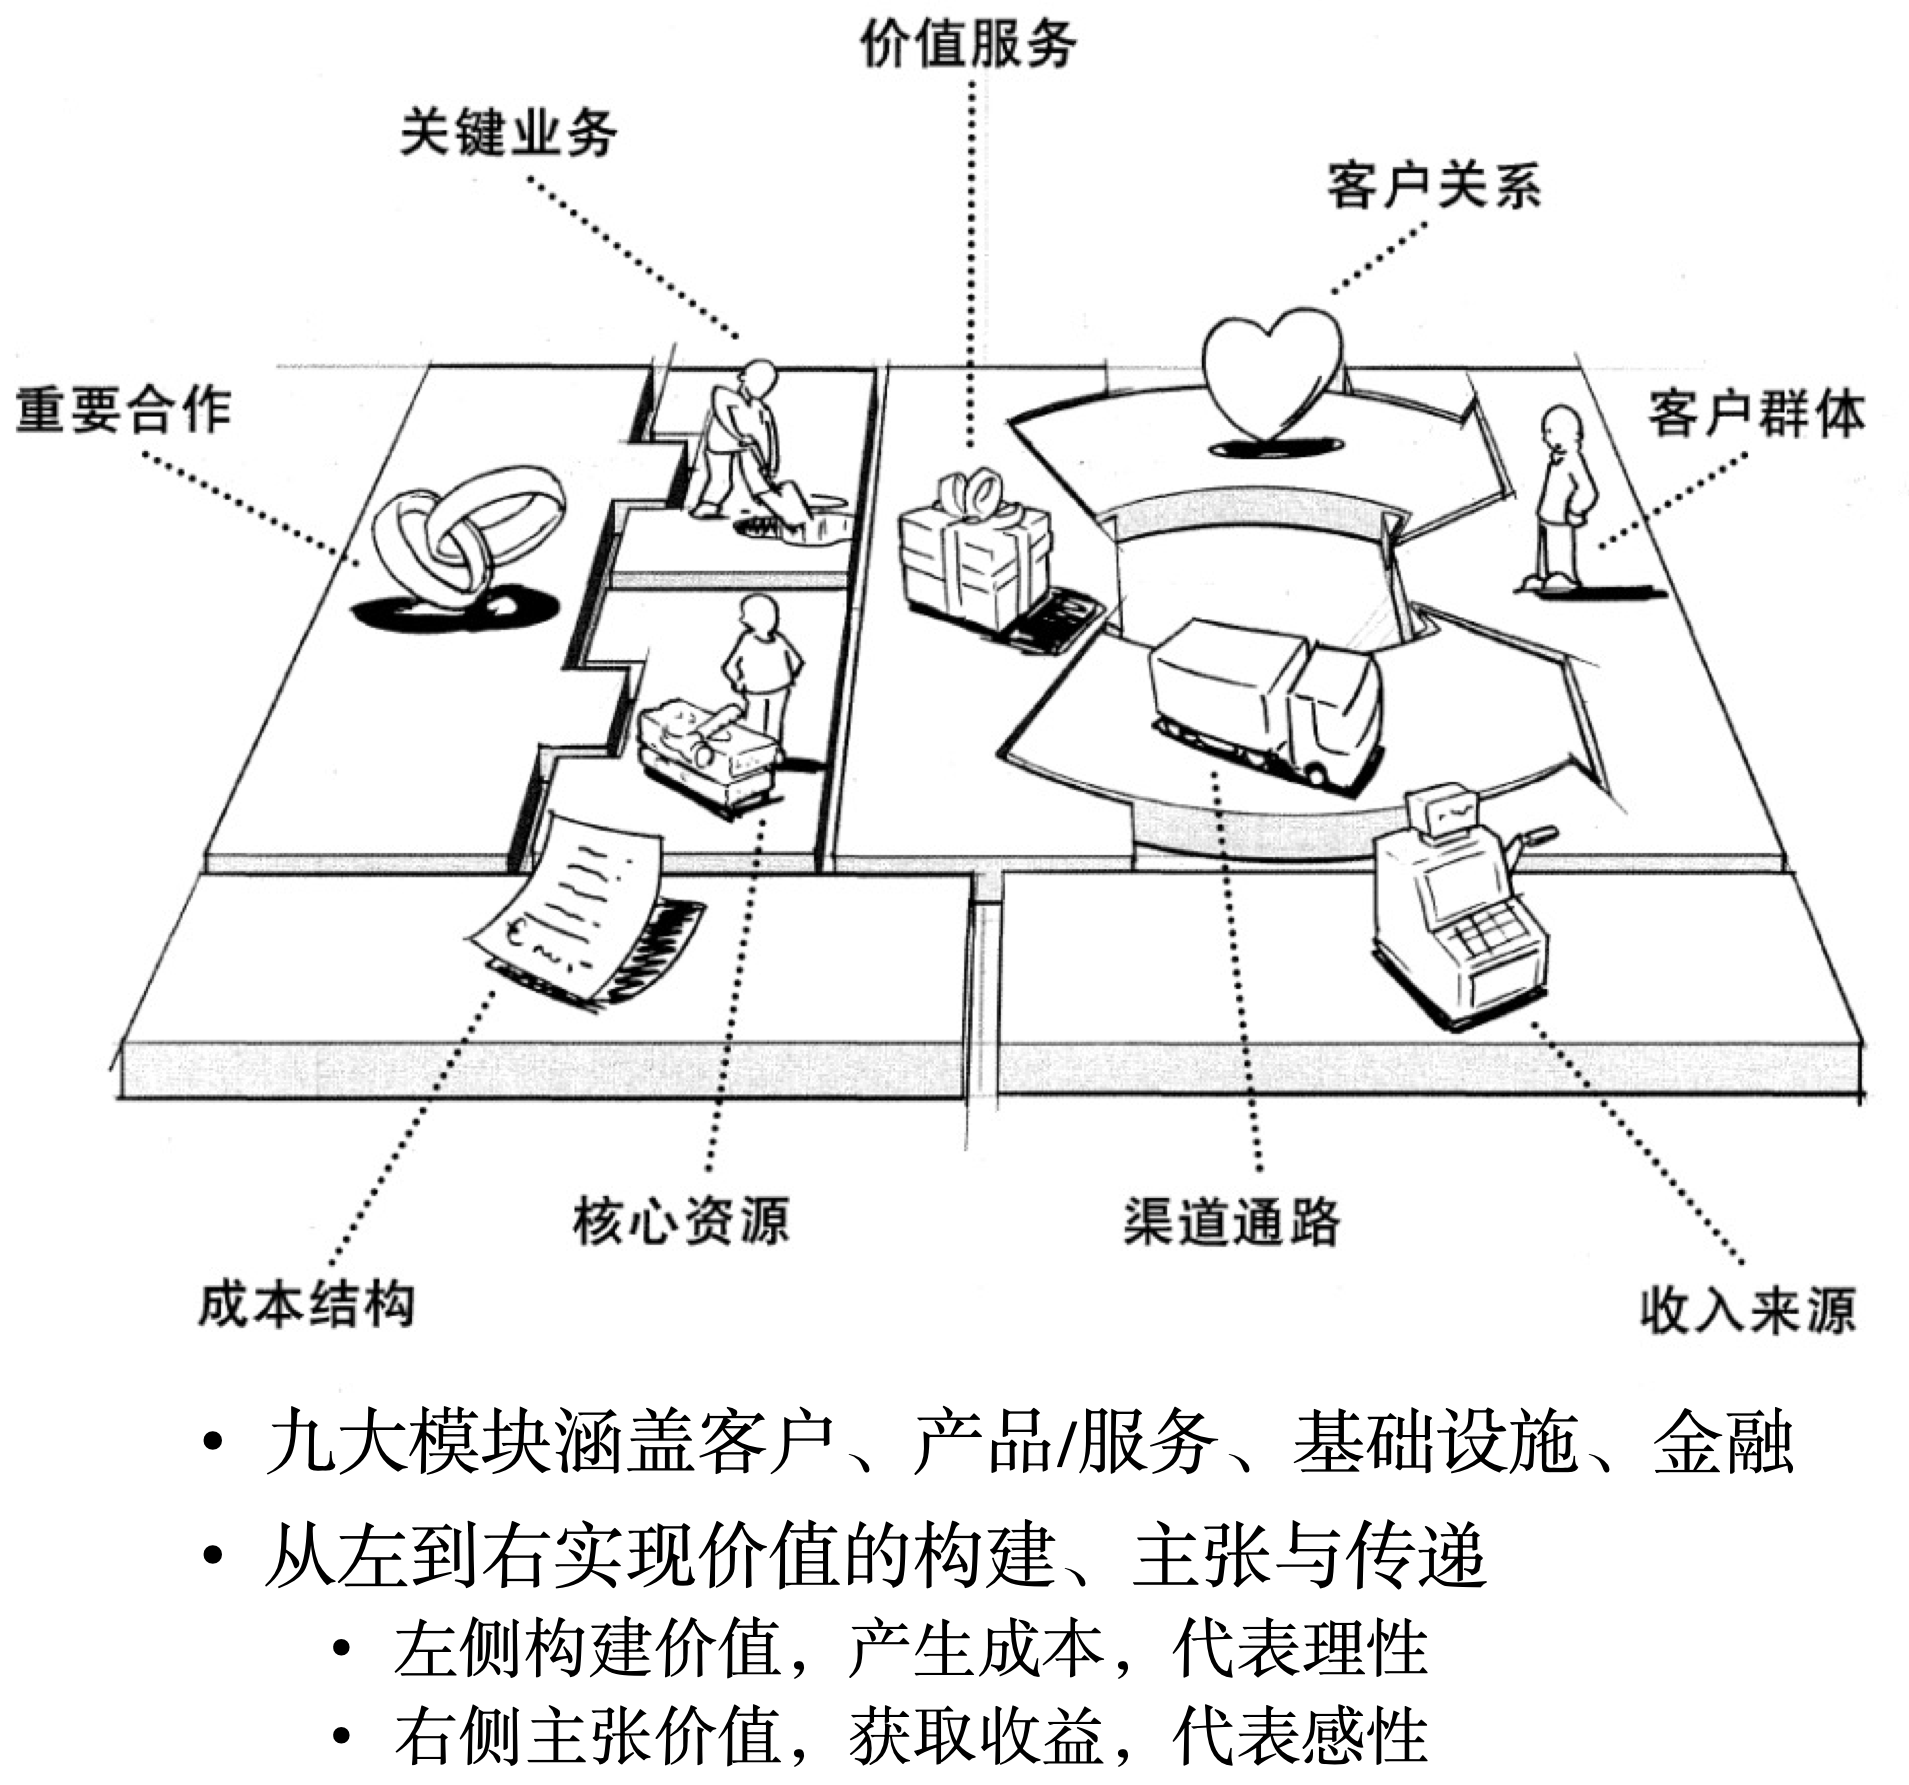
\includegraphics[width=0.58\textwidth]{img/商业模式画布.png}
		\vspace{-0.5em}
	\end{figure}
	
	\subsection{商业模式的九大模块}
	\begin{figure}[H]
		\vspace{-0.5em}
		\centering
		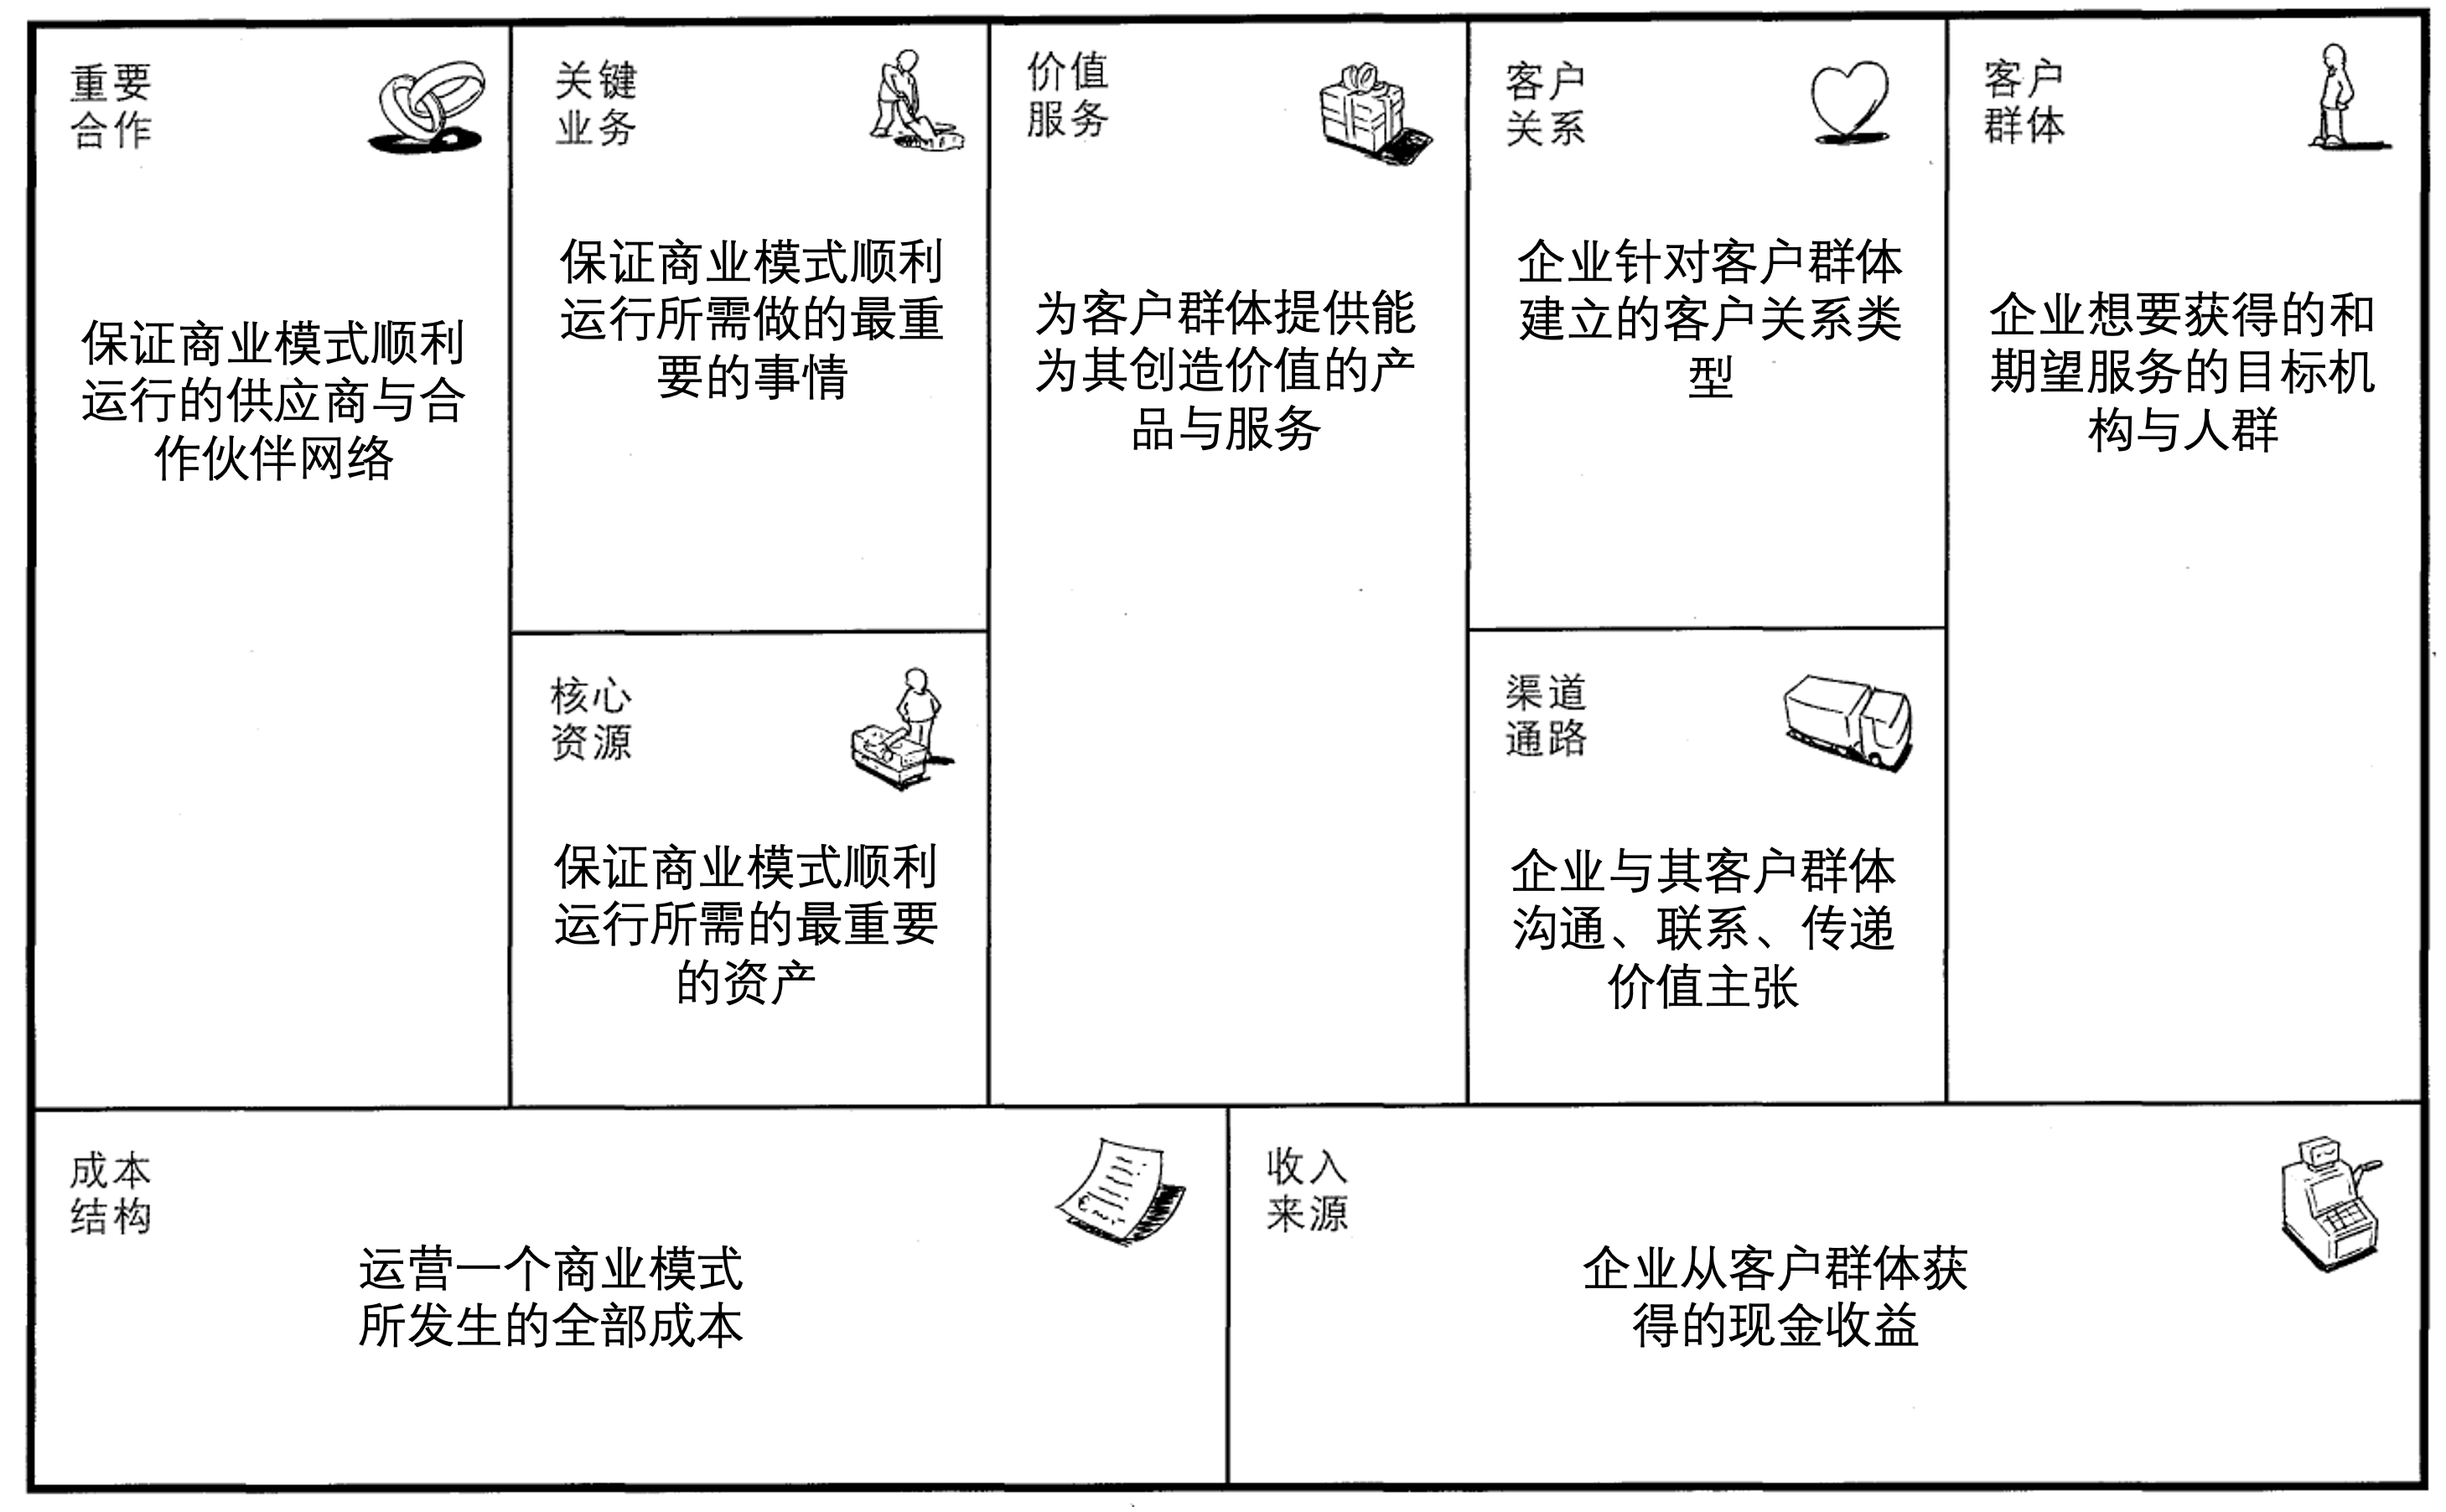
\includegraphics[width=0.72\textwidth]{img/商业模式的九大模块.png}
		\vspace{-0.5em}
	\end{figure}

	\subsubsection{客户细分}
	客户细分(customer segments)描述了一家企业想要获得的和期望服务的不同的目标人群和机构。
	\begin{itemize}
		\item 客户是任何一个商业模式的核心,为了更好地满足客户,企业应按照他们的需求、行为及特征的不同,将客户分成不同的群组。
		\item 一个组织需要谨慎地选择服务于哪个客户群体,以及忽略哪一个客户群体。
	\end{itemize}

	细分客户群体的条件:
	\begin{itemize}
		\item 他们的需求催生了一项新的供给
		\item 需要建立一个新的分销渠道
		\item 需要建立一套新的客户关系类型
		\item 他们产生的利润率显著不同
		\item 他们愿意为某方面的特殊改进而买单
	\end{itemize}


	客户群体的划分有不同的方式,例如:
	\begin{itemize}
		\item 大众市场
		\begin{itemize}
			\item 基于大众化市场的商业模式不会区分客户群体。它们的价值主张、分销渠道、客户关系聚焦于一个庞大的、有着广泛的相似需求和问题的客户群。这种商业模式常见于消费电子产业、大型零售商。
		\end{itemize}
		\item 小众市场
		\begin{itemize}
			\item 迎合的是某一个具体的、专门的客户群体。其价值主张、分销渠道和客户关系皆是根据某小众市场的具体需求量身打造的。这样的商业模式常见于供应商-采购商关系中。
		\end{itemize}
		\item 求同存异的客户群体
		\begin{itemize}
			\item 有的商业模式面向的是有些许差别的需求和问题的多个细分市场,它为每一个客户群体都提供稍有区别的价值主张,常见于各类生产线。
		\end{itemize}
		\item 多元化的客户群体
		\begin{itemize}
			\item 一个面向多元化客户的组织服务的是两个需求和问题迥异的客户群体。例如2006年亚马逊决定通过销售其“云计算”服务来使其零售业务多元化:在线存储空间和服务器点播使用。至此,亚马逊开始了一个面向新的客户群体的自我塑造:互联网公司,即提出了一项全新的价值主张。
		\end{itemize}
		\item 多边平台(多边市场)
		\begin{itemize}
			\item 有的组织服务的是两个或多个相互独立的客户群体。比如一家信用卡公司,既需要一个基数庞大的持卡人群体,又需要一个庞大的接受卡片的商家群体。
		\end{itemize}
	\end{itemize}

	\subsubsection{价值主张}
	价值主张(value propositions)描述的是为某一客户群体提供能为其创造价值的产品和服务。
	\begin{itemize}
		\item 价值主张是客户选择一家公司而放弃另一家的原因,它解决了客户的问题或满足其需求。
		\item 每一个价值主张就是一个产品和(或)服务的组合,这一组合迎合了某一客户群体的要求,价值主张是一家公司为客户提供的利益的集合或组合。
		\item 价值主张可以是创新性的,并带来一种新的或革命性的产品或服务,也可以是与既有的产品或服务相似,但增添了新的特点和属性。
	\end{itemize}

	价值主张通过针对某个群体的需求定制一套新的元素组合来为该群体创造价值,所创造的价值可以是数量上的(如价格、服务响应速度等),也可以是质量上的(如设计、客户体验)。
		
	对有益于容户价值创造的因素:
	\begin{itemize}
		\item 创新
		\begin{itemize}
			\item 有的价值主张满足的是客户之前未曾察觉的全新的需求,因为之前并没有类似的产品或服务存在。这一类经常,但并非总是与科技相关。比如手机,在移动通信中创造了一个新的产业。
		\end{itemize}
		\item 性能 
		\begin{itemize}
			\item 改进产品或服务的性能是一项传统而普遍的创造价值的方式。个人计算机产业一直以来便采用这种方式,即不断向市场提供性能更加强大的计算机。但增进性能是有局限性的。
		\end{itemize}
		\item 定制
		\begin{itemize}
			\item 针对某些客户或客户群体的某项需求提供定制的产品或服务能够创造价值。大规模定制和客户参与创造的生产方式凸显了其重要性。这种方式在提供了定制化的产品或服务的同时,保持了生产规模化的经济性。
		\end{itemize}
		\item 保姆式服务
		\begin{itemize}
			\item 帮用户完成任务并创造价值,例如劳斯莱斯提供的飞机引擎维护服务。           
		\end{itemize}
		\item 设计
		\begin{itemize}
			\item 设计是一个重要但很难量化的元素。一个产品可能由于其出色的设计而鹤立鸡群。在时尚产业和消费电子产业,设计对于价值主张而言尤其重要。
		\end{itemize}
		\item 品牌/地位
		\begin{itemize}
			\item 客户可以简单地通过使用和展示某一品牌而获得价值。例如,佩戴一块劳力士手表,彰显了财富。           
		\end{itemize}
		\item 价格
		\begin{itemize}
			\item 以更低的价格提供相同的价值是满足价格敏感型客户群体的需求的普遍方式。但低价格主张对于商业模式的其他模块都有着重要的影响例如,廉价航空专门设计了一整套商业模式来实现低成本飞行。
		\end{itemize}
		\item 缩减成本
		\begin{itemize}
			\item 帮助客户节约成本是创造价值的重要方式。例如服务外包产业。
		\end{itemize}
		\item 风险控制
		\begin{itemize}
			\item 为客户购买的产品或服务降低风险,能够为其创造价值。对于一个二手车买家而言,一年内保修的政策为买家降低了购车后的故障和维修风险。
		\end{itemize}
		\item 可获得性
		\begin{itemize}
			\item 帮助客户获得之前他们无法获得的产品和服务也是创造价值的方式。这一方式可能得益于商业模式的创新、科技的创新,或两种创新共同作用的结果。例如,奈特捷公司使得合伙购买私人飞机这种方式流行起来。
		\end{itemize}
		\item 便利性/实用性
		\begin{itemize}
			\item 让产品使用起来更方便或操作起来更简单也可以创造相当大的价值。通过iPod和iTunes,苹果公司为客户提供了数字音乐从搜索、购买,到下载和使用一整套前所未有的便捷体验。苹果也因此主导了整个数字音乐市场。
		\end{itemize}
	\end{itemize}
		
		
	\begin{itemize}
		\item 让事情更简单(痛点):价格、缩减成本、便利性/实用性
		\item 让事情更“复杂”(收益):定制、设计、品牌地位、可获得性
		\item 让事情更“透明”(痛点):风险控制、一站式服务
	\end{itemize}

	\subsubsection{渠道通路}
	渠道通路(channels)描述的是一家企业如何同它的客户群体达成沟通并建立联系,以向对方传递自身的价值主张。
	\begin{itemize}
		\item 与客户的交流、分销和销售渠道构成了一个企业的客户交互体系。
		\item 渠道通路在客户体验中扮演着重要角色的客户触点。
		\item 是商业真正的秘密,与产品设计的关系微妙(重合度小,却又容易受到产品口碑风险的冲击),容易积累收益但波动性极大、风险高。
	\end{itemize}

	渠道通路的作用包括以下几点:
	\begin{itemize}
		\item 使客户更加了解公司的产品和服务;
		\item 帮助客户评估一家公司的价值主张;
		\item 使得客户得以购买某项产品和服务;
		\item 向客户传递价值主张;
		\item 向客户提供售后支持。
	\end{itemize}


	一个组织可以选择使用自有渠道来与它的客户建立联系,也可以选择合作方的渠道,或者两者兼用。
	\begin{itemize}
		\item 自有渠道可以是直接的,比如内部销售团队或者网站;也可以是间接的,如该组织名下的或负责运营的零售商店
		\item 合作方渠道是间接的,并且范围很广,比如批发分销渠道、销售渠道或者合作方运营的网站
		\item 使用合作方渠道导致利润更低,但这些渠道可以帮助一个组织扩张客户的范围,并且从合作方的强项中获益
		\item 自有渠道尤其是直接的自有渠道利润较高,但渠道本身的建立和运营成本也会很高
		\item 难点在于整合各种类型的渠道,并找到最佳平衡,以创造最佳的客户体验和最大化的收益
	\end{itemize}
	
	\begin{figure}[H]
		\vspace{-0.5em}
		\centering
		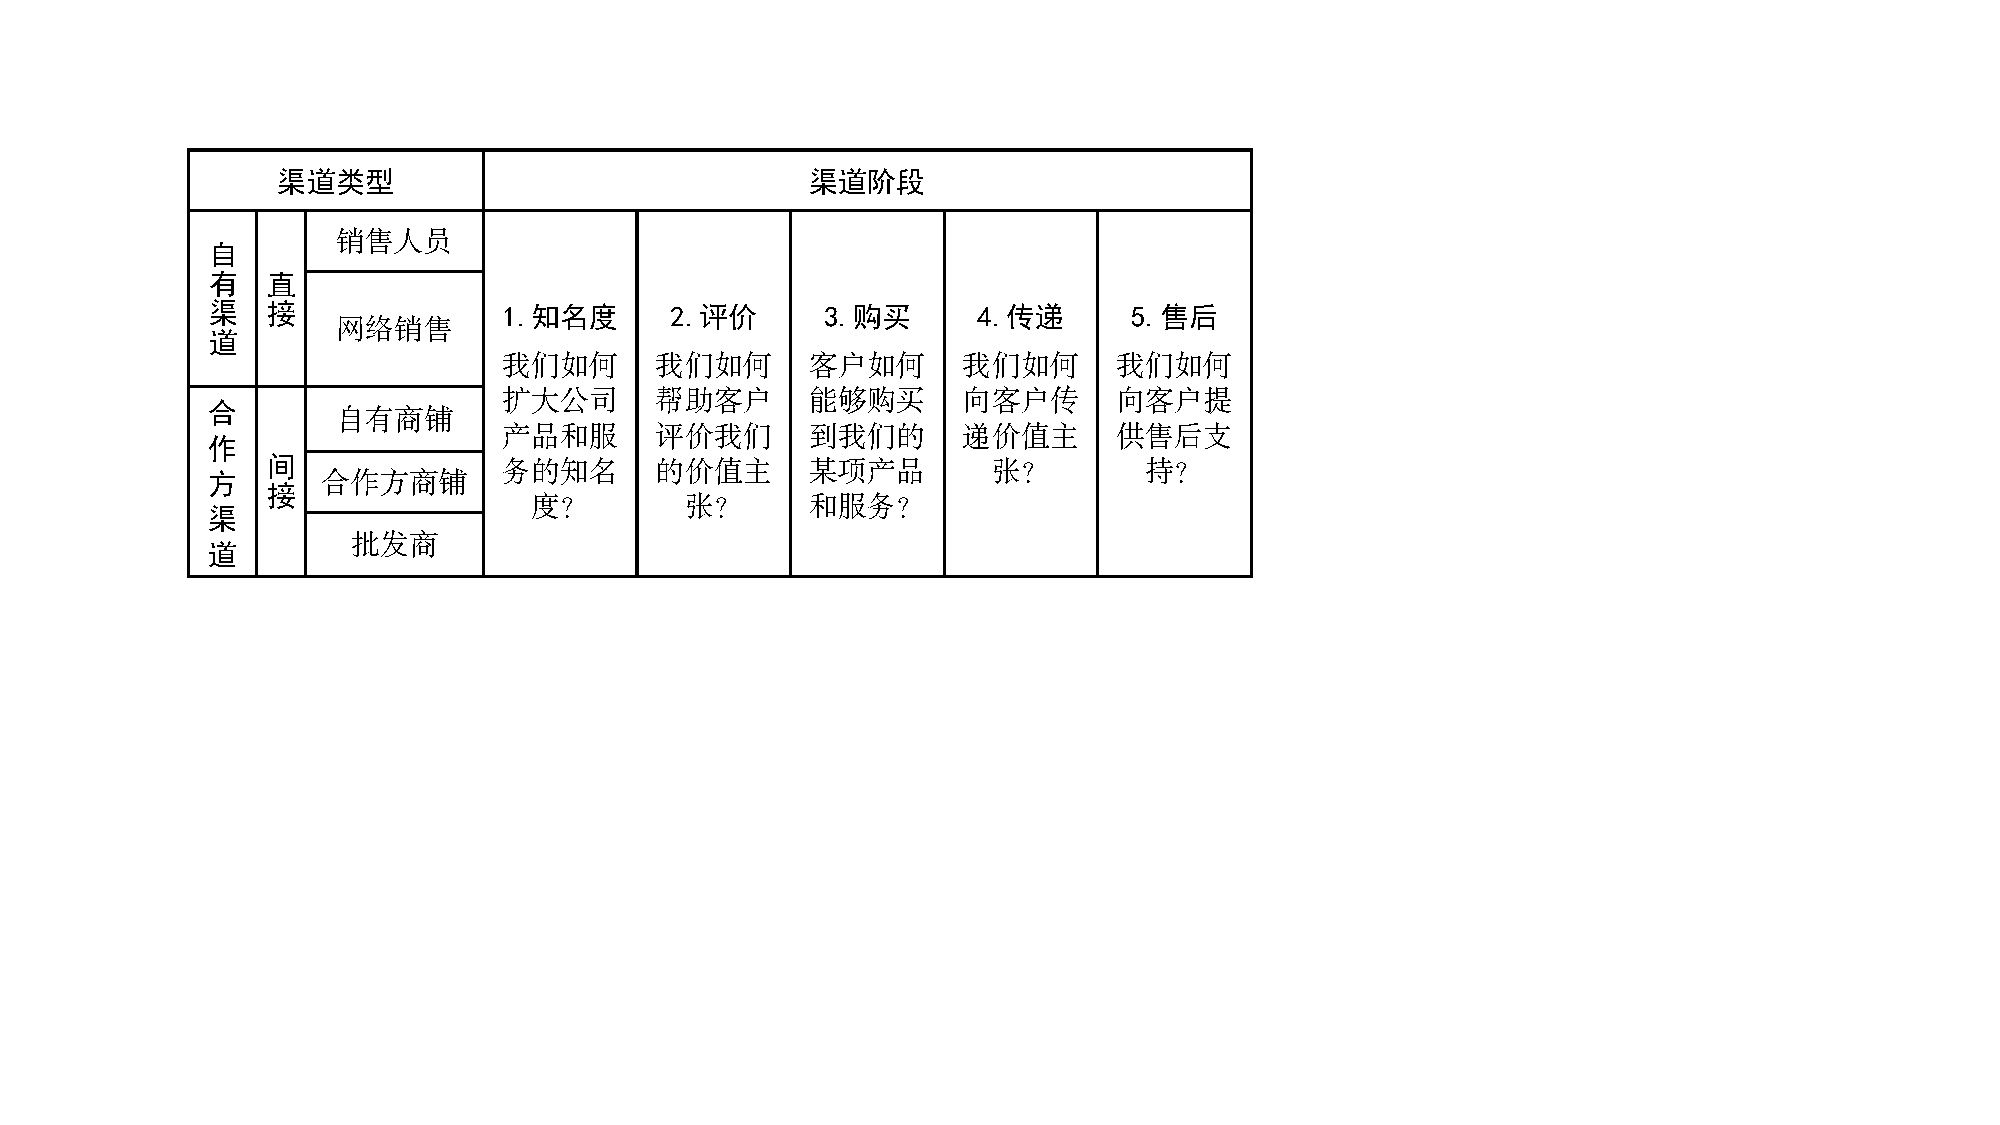
\includegraphics[width=0.7\textwidth]{img/渠道通路的类型和阶段.pdf}
		\vspace{-0.5em}
	\end{figure}

	\subsubsection{客户关系}
	客户关系(customer relationships)描述的是一家企业针对某一个客户群体所建立的客户关系的类型。
	\begin{itemize}
		\item 企业需要明确对每一个客户群体欲建立何种关系类型。
		\item 客户关系可能是由以下动机驱动的:
		\begin{itemize}
			\item 开发新的客户
			\item 留住原有客户
			\item 增加销售量(或单价)
		\end{itemize}
	\end{itemize}

	客户关系的类型:
	\begin{table}[H]
		\centering
		\begin{tabularx}{0.8\textwidth}{|l|X|}
		\hline
		客户关系       & \multicolumn{1}{c|}{具体描述}                                                                                                   \\ \hline
		私人服务       & 这种客户关系是基于人际互动的。客户可以与客户代表进行交流并在销售过程中以及购买完成之后获得相应的帮助。这种互动可以发生在购买的现场,通过呼叫中心、电邮或其他渠道进行。                                         \\ \hline
		专属私人服务     & 这种客户关系要求为每一个客户指定一个固定的客户经理。这是一种最深层的最私人的客户关系类型,通常需要很长时间的积累。例如,私人银行服务,为高净值客户指定专门的银行经理。类似的客户关系可以在其他行业中找到,比如大容户经理负责维系与重要客户的私人关系。 \\ \hline
		自助服务       & 在这种客户关系中,企业无须直接维护与客户的关系。企业只需为客户提供一切自助服务所需要的渠道。                                                                              \\ \hline
		自动化服务      & 此类型的客户关系将相对复杂的客户自助服务形式与自动化流程相结合。例如,个人在线资料使得客户可以获得定制化的服务。自动化服务可以识别客户身份及其特点,并符合预订单和交易内容的信息。最好的自动化服务可以模仿人际关系交往(比如推荐书或电影)。      \\ \hline
		社区         & 企业使用用户社区来融入客户以预判市场未来发展的方向,管理客户预期,例如花粉俱乐部、小米之家等。                                                                             \\ \hline
		与客户协作,共同创造 & 更多的企业开始超越传统的买卖关系,与客户合作共同创造价值。亚马迅邀请其客户撰写书评,如此就为其他书友创造了价值。有的企业吸引用户来帮助他们共同设计有创造性的新产品。                                          \\ \hline
		\end{tabularx}
		\end{table}

	\subsubsection{收入来源}
	收入来源(revenue streams)代表企业从每一个客户群体获得的现金收益(须从收益中扣除成本得到利润)。
	\begin{itemize}
		\item 每一个收益来源中可能包含不同的价格机制,比如固定目录价、议价、竞价、根据市场浮动的价格、根据购买数量浮动的价格,以及收益管理系统(定价)
		\item 一个商业模式可能包含的收益来源分为以下两种不同的类型:
		\begin{itemize}
			\item 交易收入由客户一次性支付产生
			\item 持续收入:因向客户传递了新的价值主张或提供了售后支持而带来的客户持续支付
		\end{itemize}
	\end{itemize}

	创造收入来源的方式有很多种:
	\begin{itemize}
		\item 资产销售
		\begin{itemize}
			\item 最普遍被认知的收入来源就是实物产品所有权的出售。例如亚马逊通过网站销售图书、音乐、消费类电子产品等商品。
		\end{itemize}
		\item 使用费
		\begin{itemize}
			\item 这一收入来源是因对某种具体服务的使用而产生的。对该服务使用得越多,消费者支付的就越多。例如电信运营商根据用户使用电话的分钟数收费。
		\end{itemize}
		\item 会员费
		\begin{itemize}
			\item 这种收入来源通过向用户销售某项服务持续的使用权限实现。例如健身房向用户销售月卡或年卡以限定会员对健身器材的使用时限。
		\end{itemize}
		\item 租赁
		\begin{itemize}
			\item 这种收入来源产生于:将某一特定资产在某一个时期专门供给某人使用并收取一定费用。对出租者而言,这种做法提供的是经常性收入。同时对于租赁者而言,仅需要承担一个限定时间内的费用而无须承担整个所有权所耗费的成本。
		\end{itemize}
		\item 许可使用费
		\begin{itemize}
			\item 这种收入来源来自:向用户授予某种受保护知识产权的使用权,并向其收取许可使用费。许可使用费使得资源持有者无须生产产品或进行任何商业化操作,而仅凭其对资源的所有权获取收益。许可使用费在传媒行业十分常见,内容所有人会持有版权,但是将使用权提供给第三方。相似地,在科技产业中,专利持有者将专利使用权提供给其他公司使用并收取专利使用费。
		\end{itemize}
		\item 经纪人佣金
		\begin{itemize}
			\item 这一收入来源于向双方或多方提供的中介服务。例如,信用卡发卡机构针对每一笔交易向商家和持卡人按交易额度的一定百分比收取费用。
		\end{itemize}
		\item 广告费
		\begin{itemize}
			\item 这种收入来源来自为某种产品、服务或品牌做广告的费用。传统的传媒业和活动策划的收入很大程度上依赖于广告上的收人。近此年其他产业,包括软件业和服务业,也开始更多地依赖于广告收入。
		\end{itemize}
	\end{itemize}

	定价机制:
	\begin{table}[H]
		\centering
		\resizebox{\textwidth}{!}{
		\begin{tabular}{|c|l|c|l|}
		\hline
		\multicolumn{2}{|c|}{\begin{tabular}[c]{@{}c@{}}\textbf{固定价格}\\ 基于静态变量预定的价格\end{tabular}} & \multicolumn{2}{c|}{\begin{tabular}[c]{@{}c@{}}\textbf{浮动价格}\\ 价格依据市场条件变化\end{tabular}}             \\ \hline
		目录价        & \begin{tabular}[c]{@{}l@{}}对个别产品、服务或其他价值主\\ 张设定的固定价格\end{tabular}   & 谈判(议价) & \begin{tabular}[c]{@{}l@{}}双方或多方的价格谈判,取决于谈判\\ 各方的谈判能力和技巧\end{tabular}             \\ \hline
		基于产品特性的    & \begin{tabular}[c]{@{}l@{}}基于某项价值主张的数量或质量的\\ 定价\end{tabular}        & 收益管理   & \begin{tabular}[c]{@{}l@{}}价格基于库存及发生购买的时间\\ (通常用于易耗资源,如宾馆房间和\\ 航班机位)\end{tabular} \\ \hline
		基于客户群的     & \begin{tabular}[c]{@{}l@{}}基于某一客户群体的类型和特征\\ 的定价\end{tabular}        & 实时市场价格 & 价格根据需求变化动态变动                                                                      \\ \hline
		基于数量的      & 基于购买数量的定价                                                           & 拍卖     & 根据竞价的结果决定                                                                         \\ \hline
		\end{tabular}
		}
		\end{table}

	\subsubsection{核心资源}
	核心资源(key resources)描述的是保证一个商业模式顺利运行所需的最重要的资产。
	\begin{itemize}
		\item 每一种商业模式都需要一些核心资源。这些资源使得企业得以创造并提供价值主张,获得市场,保持与某个客户群体的客户关系并获得收益。
		\item 核心资源可包括实物资源、金融资源、知识性资源以及人力资源。核心资源可以是自有的,也可以通过租赁获得,或者从重要合作伙伴处获得。
	\end{itemize}

	核心资源可以分为如下几类:
	\begin{itemize}
		\item 实物资源
		\begin{itemize}
			\item 这一范畴包括实物资产,如生产设备、房屋、车辆、机器、系统、销售点管理系统及分销渠道。作为零售商,沃尔玛和亚马逊都非常依赖实物资源,这些资源通常都是资本密集型的。沃尔玛在全球范围内拥有庞大的仓储网络以及配套的物流设备。亚马逊拥有一套庞大的IT、仓储及物流基础设施。
		\end{itemize}
		\item 知识性资源
		\begin{itemize}
			\item 知识性资源如品牌、专营权、专利权、版权、合作关系以及客户数据库在一个强大的商业模式中扮演着越来越重要的角色。
		\end{itemize}
		\item 人力资源
		\begin{itemize}
			\item 每一家企业都需要人力资源,但人力资源对于某些商业模式而言却是尤其重要的。例如,在知识密集型产业和创新产业中,人力资源就是最关键的。
		\end{itemize}
		\item 金融资源
		\begin{itemize}
			\item 有些商业模式依赖金融资源或金融保障,比如现金、信用额度或者用于吸引关键雇员的股票期权池。例如,电信运营商爱立信在自己的商业模式中加入了金融杠杆。爱立信可以选择向银行或资本市场融资,然后将收益的一部分为购买设备的客户提供卖方融资,这就更好地保证了订单落入爱立信而非竞争对手手中。
		\end{itemize}
	\end{itemize}


	\subsubsection{关键业务}
	关键业务(key activities)描述的是保障其商业模式正常运行所需要做的最重要的事情。
	\begin{itemize}
		\item 每一个商业模式都有着一系列的关键业务,这些业务是一个企业成功运营所必须采取的最重要的行动。
		\item 同核心资源一样,它们是企业为创造和提供值主张、获得市场、维系客户关系以及获得收益所必需的,关键业务也因不同的商业模式类型而异。
		\item 对于软件商微软而言,关键业务就是软件开发;对于个人电脑生产商戴尔而言,关键业务则包含了供应链管理;对于咨询公司麦肯锡而言,关键业务包括了解决方案的提供。
	\end{itemize}

	关键业务可以分为如下几类:
	\begin{itemize}
		\item 生产
		\begin{itemize}
			\item 这些活动涉及以较大的数量或上乘的质量,设计、制造以及分销产品。生产活动在制造企业的商业模式中占支配地位。
		\end{itemize}
		\item 解决方案
		\begin{itemize}
			\item 这个类型的关键活动涉及为个体客户的问题提供新的解决方案。咨询公司、医院及其他服务性机构的运营,就是典型地受解决问题相关的活动支配的例子。这类商业模式需要的活动包括知识管理以及持续的培训等。
		\end{itemize}
		\item 平台/网络
		\begin{itemize}
			\item 在将平台作为关键资源的商业模式中,与平台以及网络相关的关键活动占据着支配地位。网络、配对平台、软件甚至品牌都可以发挥平台的作用。Visa公司为Visa$^\circledR$信用卡的商家、持卡人及银行之间搭建的交易平台,该公司的商业模式要求公司的关键活动与该平台相关。微软的商业模式要求其对其他商家的软件和Windows$^\circledR$操作系统的交互界面进行管理。这个类型的关键活动涉及了平台管理、新服务的启动以及平台的升级。
		\end{itemize}
	\end{itemize}


	\subsubsection{重要合作}
	重要合作(key partnerships)描述的是保证一个商业模式顺利运行所需的供应商和合作伙伴网络。

	可以将重要合作分为以下四种不同的类型:
	\begin{enumerate}[label=\arabic*.]
		\item 非竞争者之间的战略联盟
		\item 合作:竞争者之间的战略合作
		\item 为新业务建立合资公司
		\item 为保证可靠的供应而建立的供应商和采购商关系
	\end{enumerate}

	建立合作伙伴关系的三种动机:
	\begin{itemize}
		\item 优化及规模效应
		\begin{itemize}
			\item 最基本的一种合作关系或者买卖关系的类型就是以优化资源以及活动的配置为目的的。要一家公司拥有全部所需的资源并亲自完成所有的生产、服务环节并不合理。此类合作关系的建立通常是为了降低成本,主要采取外包或基础设施共享的形式。
		\end{itemize}
		\item 降低风险和不确定性
		\begin{itemize}
			\item 竞争环境以不确定性为特征,合作关系的建立可以帮助企业在竞争环境中降低风险。互为竞争对手的企业在某一个领域建立战略联盟,而在其他领域保持竞争关系的做法是很常见的。例如,蓝光技术是由一组全球领先的消费电子、个人电脑及内容提供商联合开发的光盘格式。各商家一方面联手向市场推出蓝光技术,另一方面又在蓝光产品的销售领域相互竞争。
		\end{itemize}
		\item 特殊资源及活动的获得
		\begin{itemize}
			\item 很少有公司拥有其商业模式下所需要的全部资源或者选择亲自完成所有的生产服务活动。更多的情况下,它们通过依赖其他占有某项资源或专注于某种生产活动的公司来实现其能力的拓展。这种类型的合作关系的动机在于获得知识、获得某种资质或者接近某个客户群体。例如,一个移动电话生产商,会选择为它们的手机搭载一个操作系统,而不会选择自主研发。
		\end{itemize}
	\end{itemize}

	\subsubsection{成本结构}
	成本结构(cost structure)描述的是运营一个商业模式所发生的全部成本。
	\begin{itemize}
		\item 创造和传递价值,维护客户关系,以及创造收益都会发生成本
		\item 在确定了核心资源、关键业务以及重要合作的情况下,成本核算就会变得相对容易
		\item 也有以低成本结构为核心的商业模式
	\end{itemize}

	商业模式的成本结构可以宽泛地分为两个等级
	\begin{itemize}
		\item 成本导向:聚焦于最大限度将成本最小化,目标在于创造并维持极尽极简的成本结构
		\item 价值导向:有些企业在商业模式设计中,更少关注成本,而更多地关注价值创造。通常更高端的价值主张以及高度的个性化服务是价值导向商业模式的特点。
	\end{itemize}

	成本结构有以下特点:
	\begin{itemize}
		\item 固定成本
		\begin{itemize}
			\item 不因产品及服务的产量而改变的成本,包括员工工资、租金、生产设备有的商业项目,比如生产型企业,以高比例的固定成本为特点。
		\end{itemize}
		\item 可变成本
		\begin{itemize}
			\item 随着产品及服务的产量而同比例变化的成本。有的商业项目,比如音乐节,以高比例的可变成本为特征。
		\end{itemize}
		\item 规模经济
		\begin{itemize}
			\item 企业的产出扩大,会带来成本优势例如,大型企业享有大宗商品采购价。诸如此类的因素导致随着总产出的增加,平均单位成本的降低。
		\end{itemize}
		\item 范围经济
		\begin{itemize}
			\item 企业的经营范围扩大,会带来成本优势。例如,在大型企业中,同一个营销活动或分销渠道上可以供多个产品使用。
		\end{itemize}
	\end{itemize}

	\subsection{苹果公司iPod/iTunes商业模式}
	\begin{figure}[H]
		\centering
		\vspace{-0.5em}
		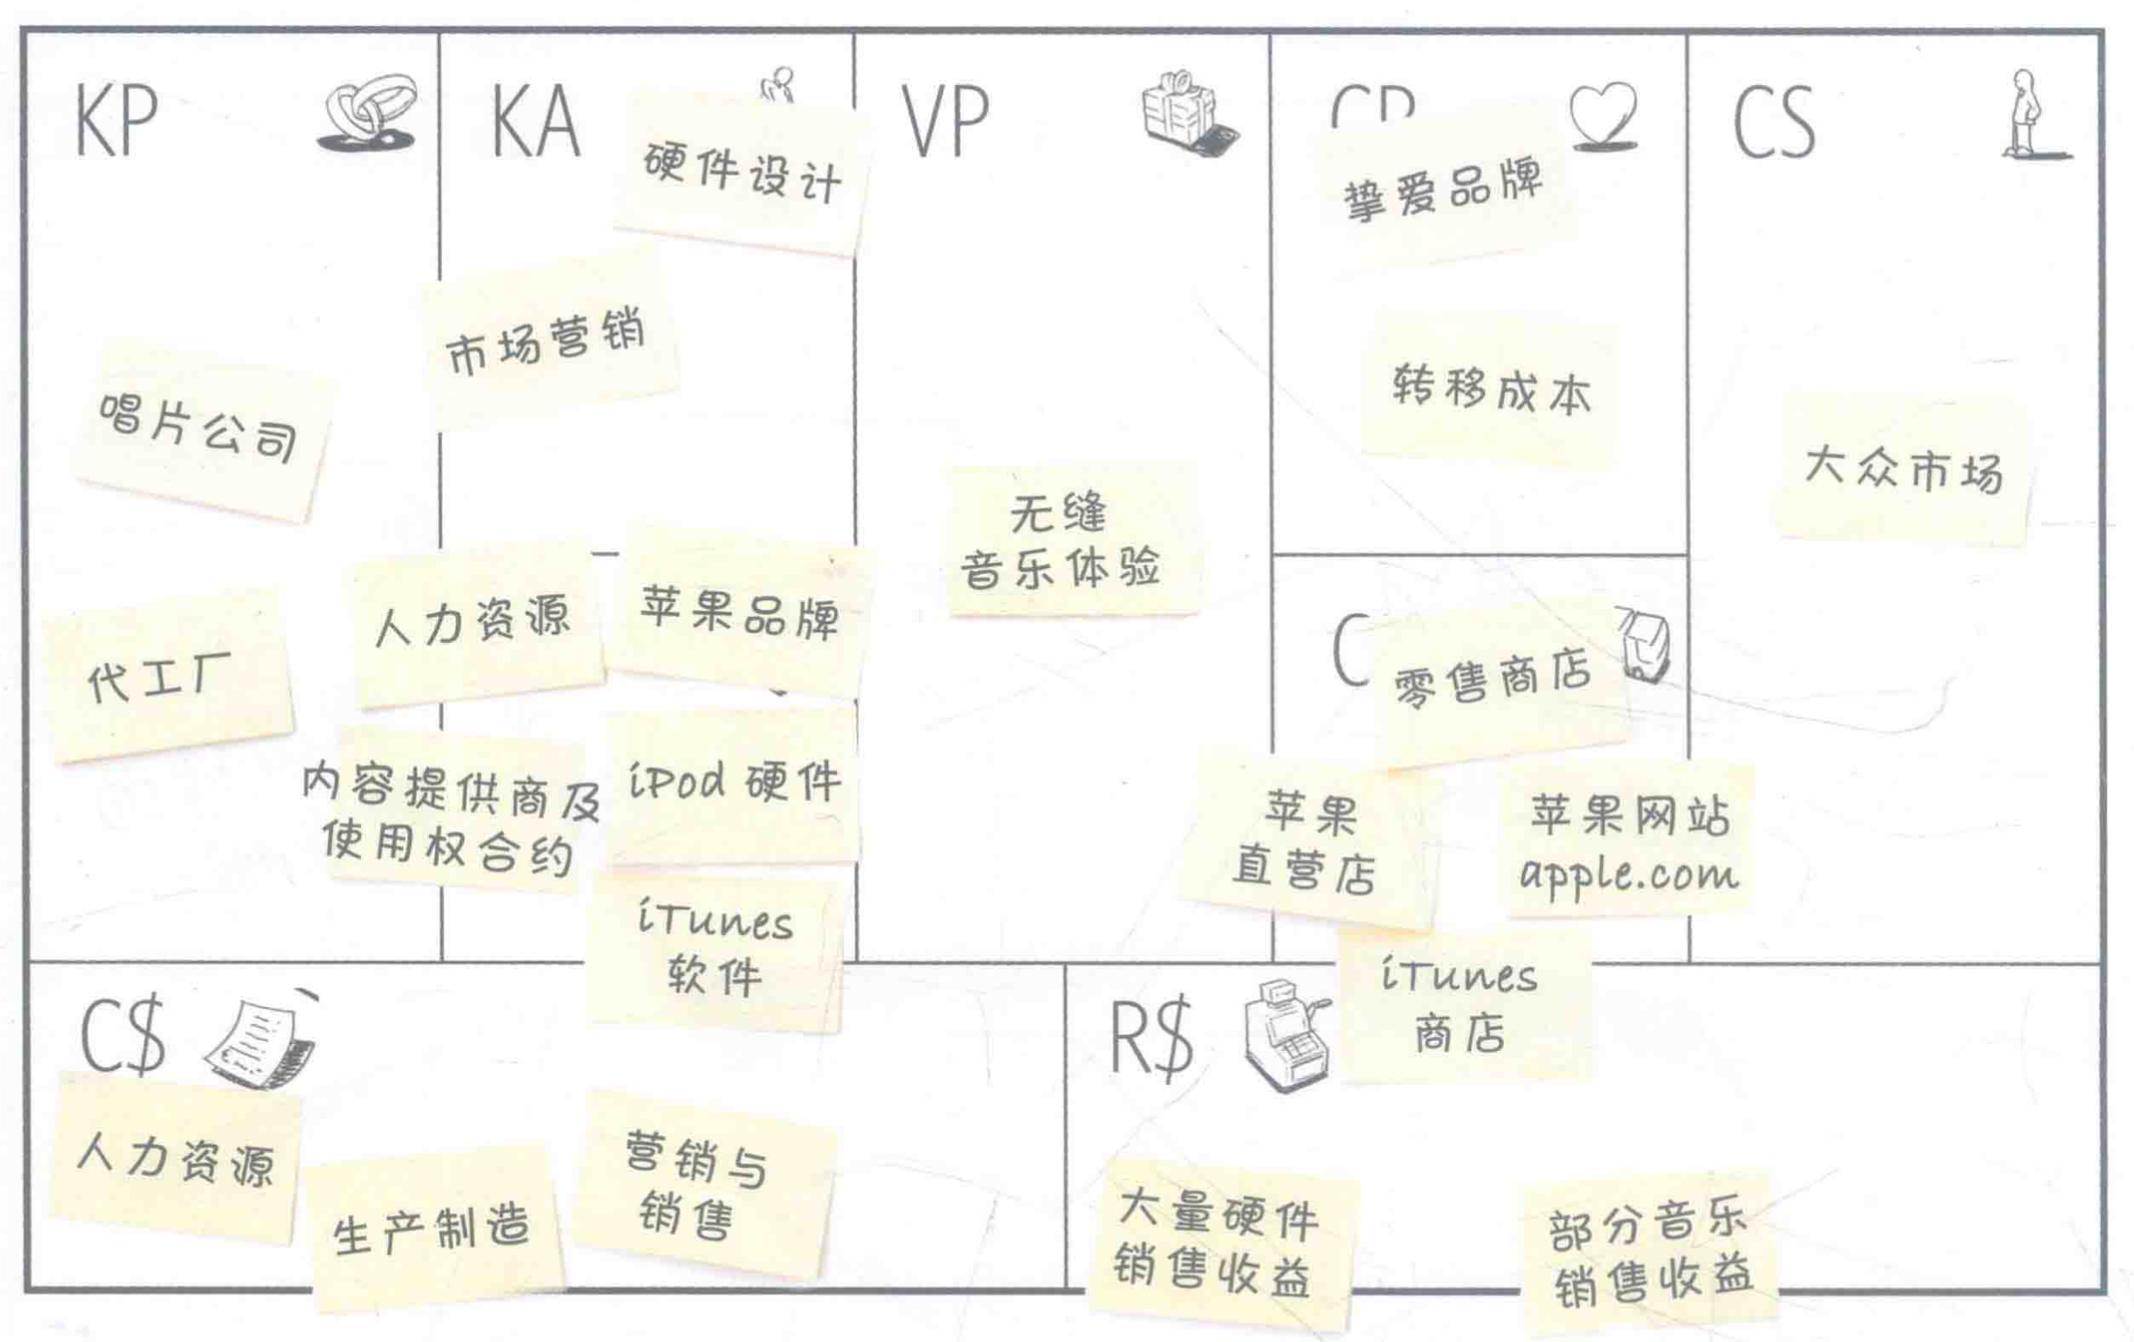
\includegraphics[width=0.8\textwidth]{img/iPod:iTunes商业模式.png}
		\vspace{-0.5em}
	\end{figure}

	\subsection{商业模式画布的使用}
	\begin{itemize}
		\item 帮助找到企业自身定位,具象化公司现有的商业模式以及未来适用的商业模式
		\item 帮助企业策划其自身的转型及退出企业的过程
		\item 帮助艺术家、文化产业生产企业以及游戏设计师设计文化创意产业的创新商业模式
		\item 帮助非营利项目组建过程中的领导团队的设计及编排
		\item 帮助将所有的项目成员以可视化的方式列出,包括全局角色、重要程度和任务依赖性
		\item 帮助评估以个体为单位的商业模式
		\item 帮助处于起步阶段的而企业家,将他们的商业计划转变成实现计划需要执行的活动
	\end{itemize}



	\section{商业模式类型}
所关注的五种商业模式类型:
\begin{itemize}
    \item 分拆商业模式
    \item 长尾商业模式
    \item 多边平台商业模式
    \item 免费商业模式
    \item 开放式商业模式
\end{itemize}

\subsection{分拆商业模式}

企业内部存在三类规则:经济、竞争与文化规则
\begin{itemize}
    \item 由此可以区分三种活动:客户关系管理、新产品开发、基础设施管理
    \item 上述三种活动对应三种价值信条:亲近顾客、产品领先、运营卓越
    \item 但这三类活动驱动因素不同,彼此之间冲突,企业内部存在不必要的消长
    \begin{itemize}
        \item 解决办法:分拆,各自独立
    \end{itemize}
\end{itemize}

\begin{table}[H]
    \centering
    \resizebox{\textwidth}{!}{
    \begin{tabular}{|l|l|l|l|}
    \hline
         & \multicolumn{1}{c|}{新产品开发}                                          & \multicolumn{1}{c|}{客户关系管理}                                                   & \multicolumn{1}{c|}{基础设施管理}                                                  \\ \hline
    经济规则 & \begin{tabular}[c]{@{}l@{}}早期市场进入获得高溢价和\\ 大量市场份额:速度是关键\end{tabular} & \begin{tabular}[c]{@{}l@{}}高昂的客户开发成本要求从\\ 每个客户手中获取高份额:\\ 范围经济是关键\end{tabular} & \begin{tabular}[c]{@{}l@{}}高固定成本使得高产量成为获\\ 得低单位成本的关键:规模经\\ 济是关键\end{tabular} \\ \hline
    竞争规则 & \begin{tabular}[c]{@{}l@{}}能力之争,进入门槛低:大\\ 量小玩家争奇斗艳\end{tabular}     & \begin{tabular}[c]{@{}l@{}}范围之争:少量的大玩家主\\ 导市场\end{tabular}                    & \begin{tabular}[c]{@{}l@{}}规模之争:迅速固化的市场;\\ 少量大玩家主导市场\end{tabular}            \\ \hline
    文化规则 & \begin{tabular}[c]{@{}l@{}}以雇员为中心:呵护创意明\\ 星\end{tabular}            & \begin{tabular}[c]{@{}l@{}}高度服务导向:顾客第一心\\ 态\end{tabular}                      & \begin{tabular}[c]{@{}l@{}}聚焦成本:强调标准化、可预\\ 期性和生产效率\end{tabular}              \\ \hline
    \end{tabular}
    }
    \end{table}

    \subsubsection{传统私人银行商业模式及其中的消长}
    \begin{figure}[H]
		\centering
        \vspace{-0.5em}
		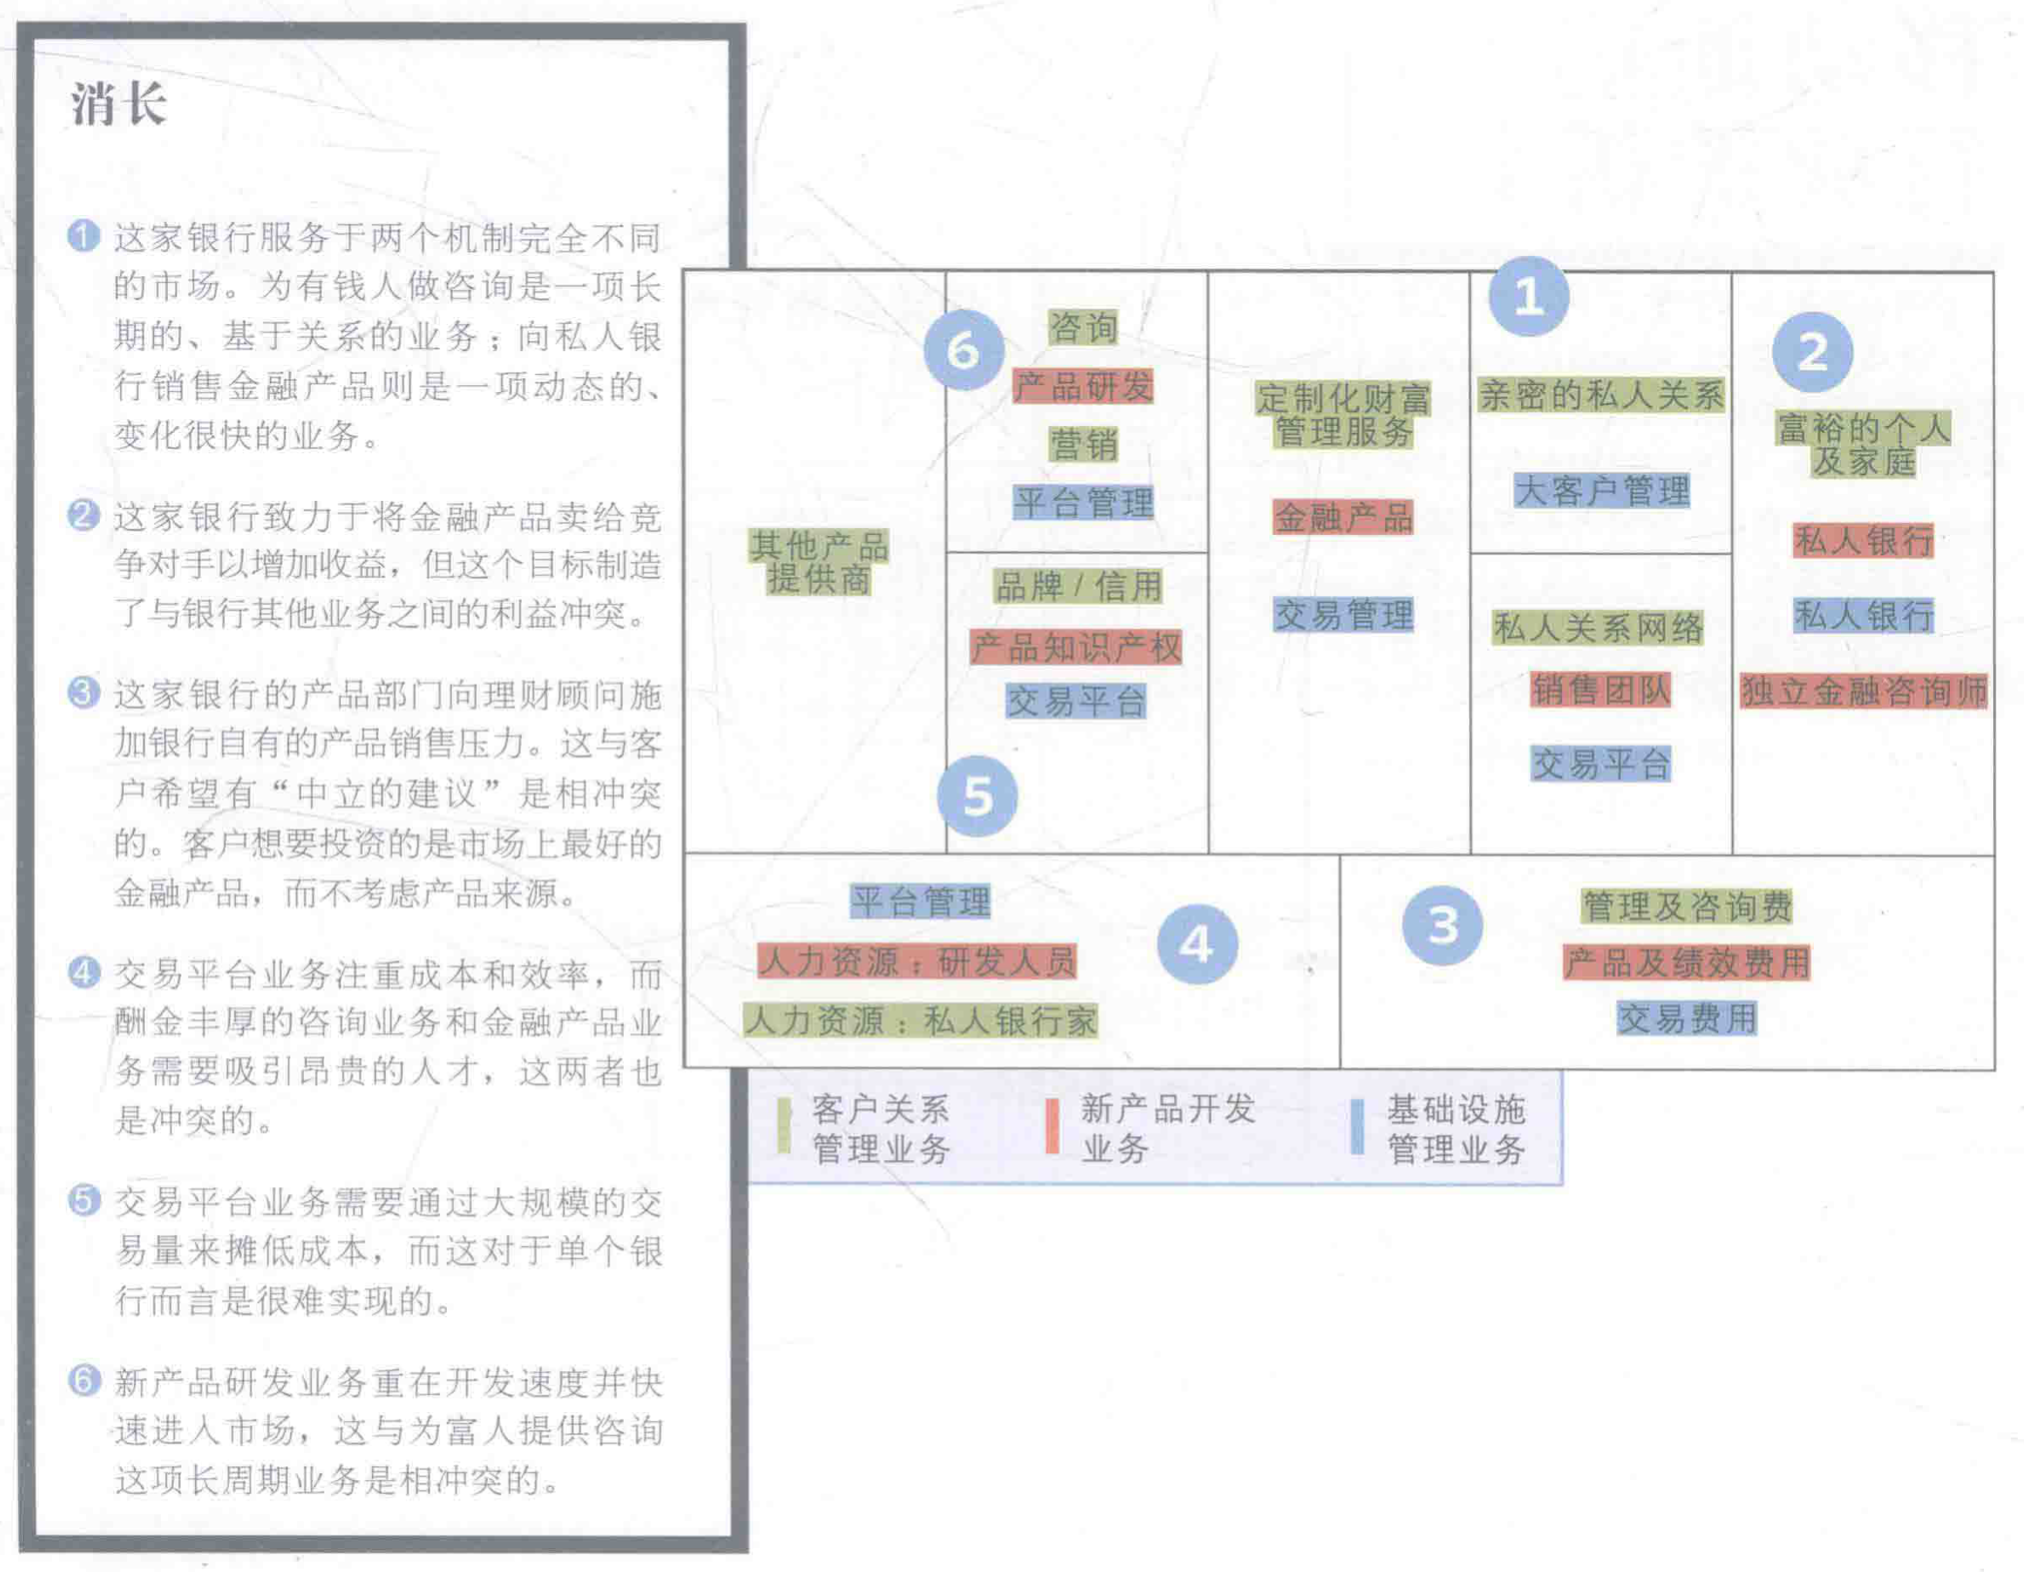
\includegraphics[width=0.95\textwidth]{img/传统私人银行商业模式及其中的消长.png}
        \vspace{-0.5em}
	\end{figure}


    \subsubsection{移动通信行业的拆分}
    移动通信企业已经为自己的商业模式松绑。传统的移动通信企业针对网络质量展开竟争,而现在它们却与竞争对手达成网络共享协议或者将网络运营业务外包给设备生产厂家。因为它们意识到它们的核心资产已经不再是网络本身,而是它们的品牌和客户关系。
    \begin{figure}[H]
		\centering
        \vspace{-0.5em}
		\includegraphics[width=\textwidth]{img/移动通信行业的拆分.png}
        \vspace{-0.5em}
	\end{figure}

    拆分后三个独立的商业模式
    \begin{figure}[H]
		\centering
        \vspace{-0.5em}
		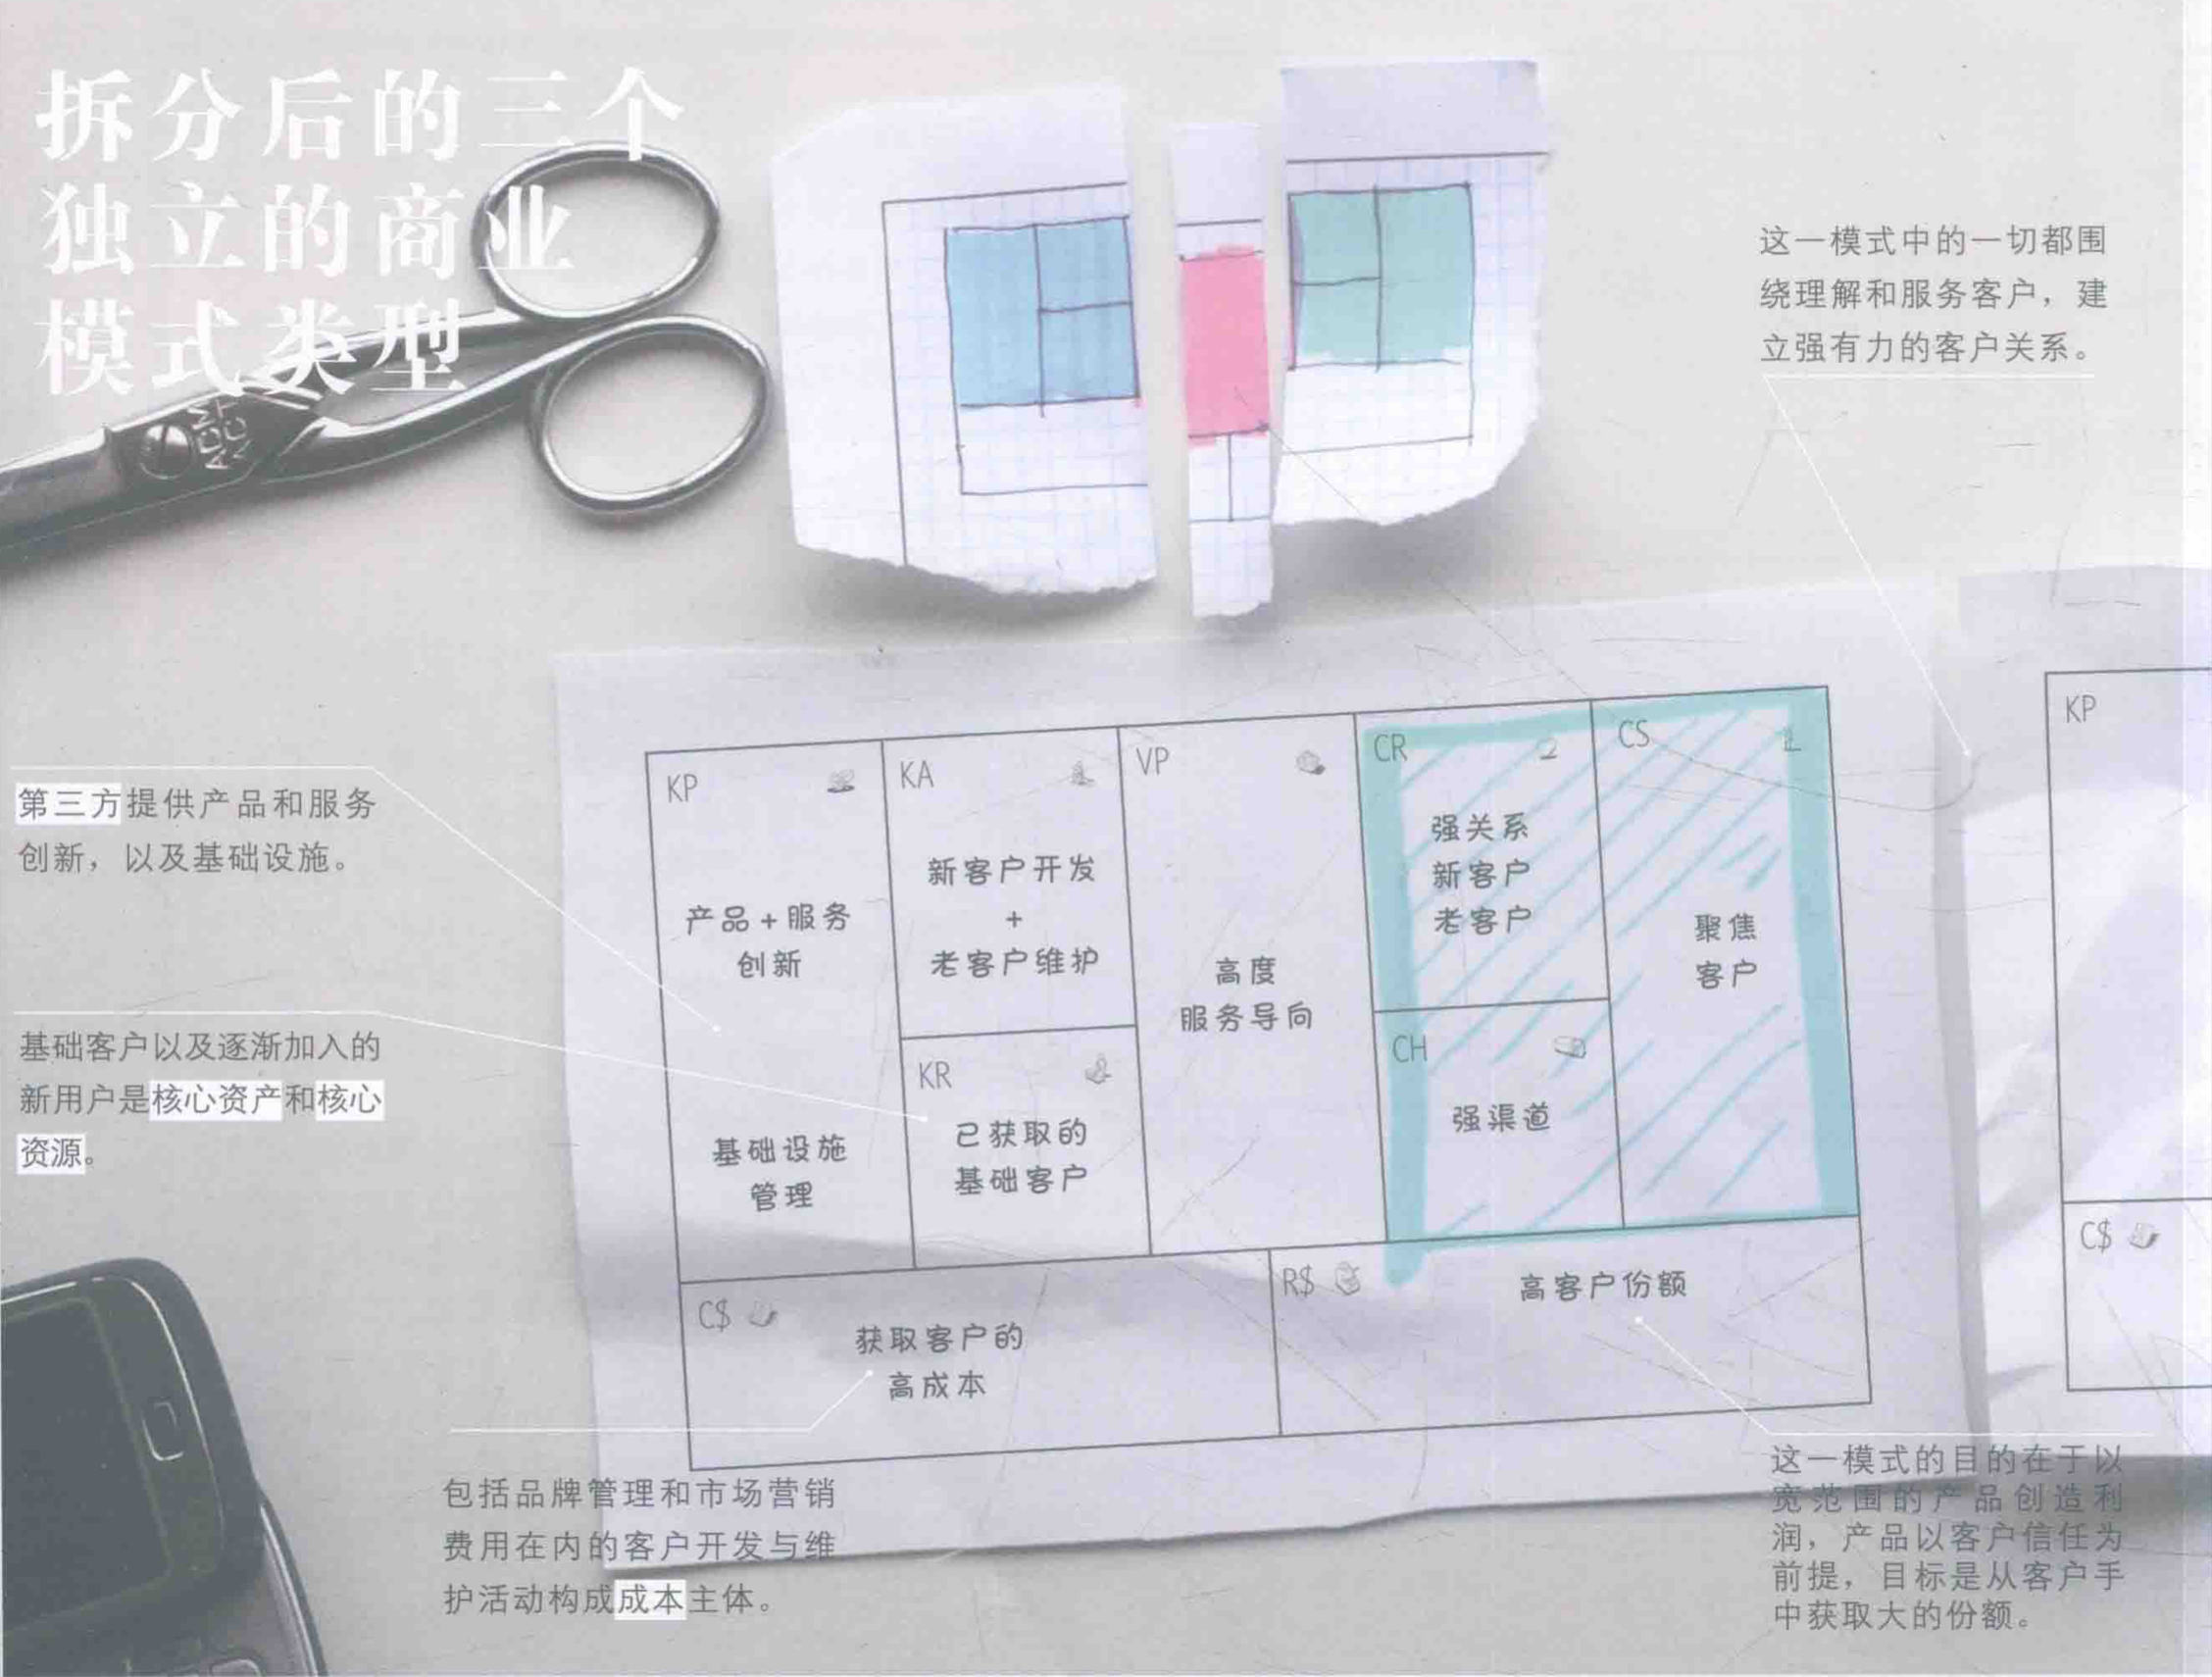
\includegraphics[width=\textwidth]{img/拆分后三个独立的商业模式1.png}
        \vspace{-0.5em}
	\end{figure}

    \begin{figure}[H]
		\centering
        \vspace{-0.5em}
		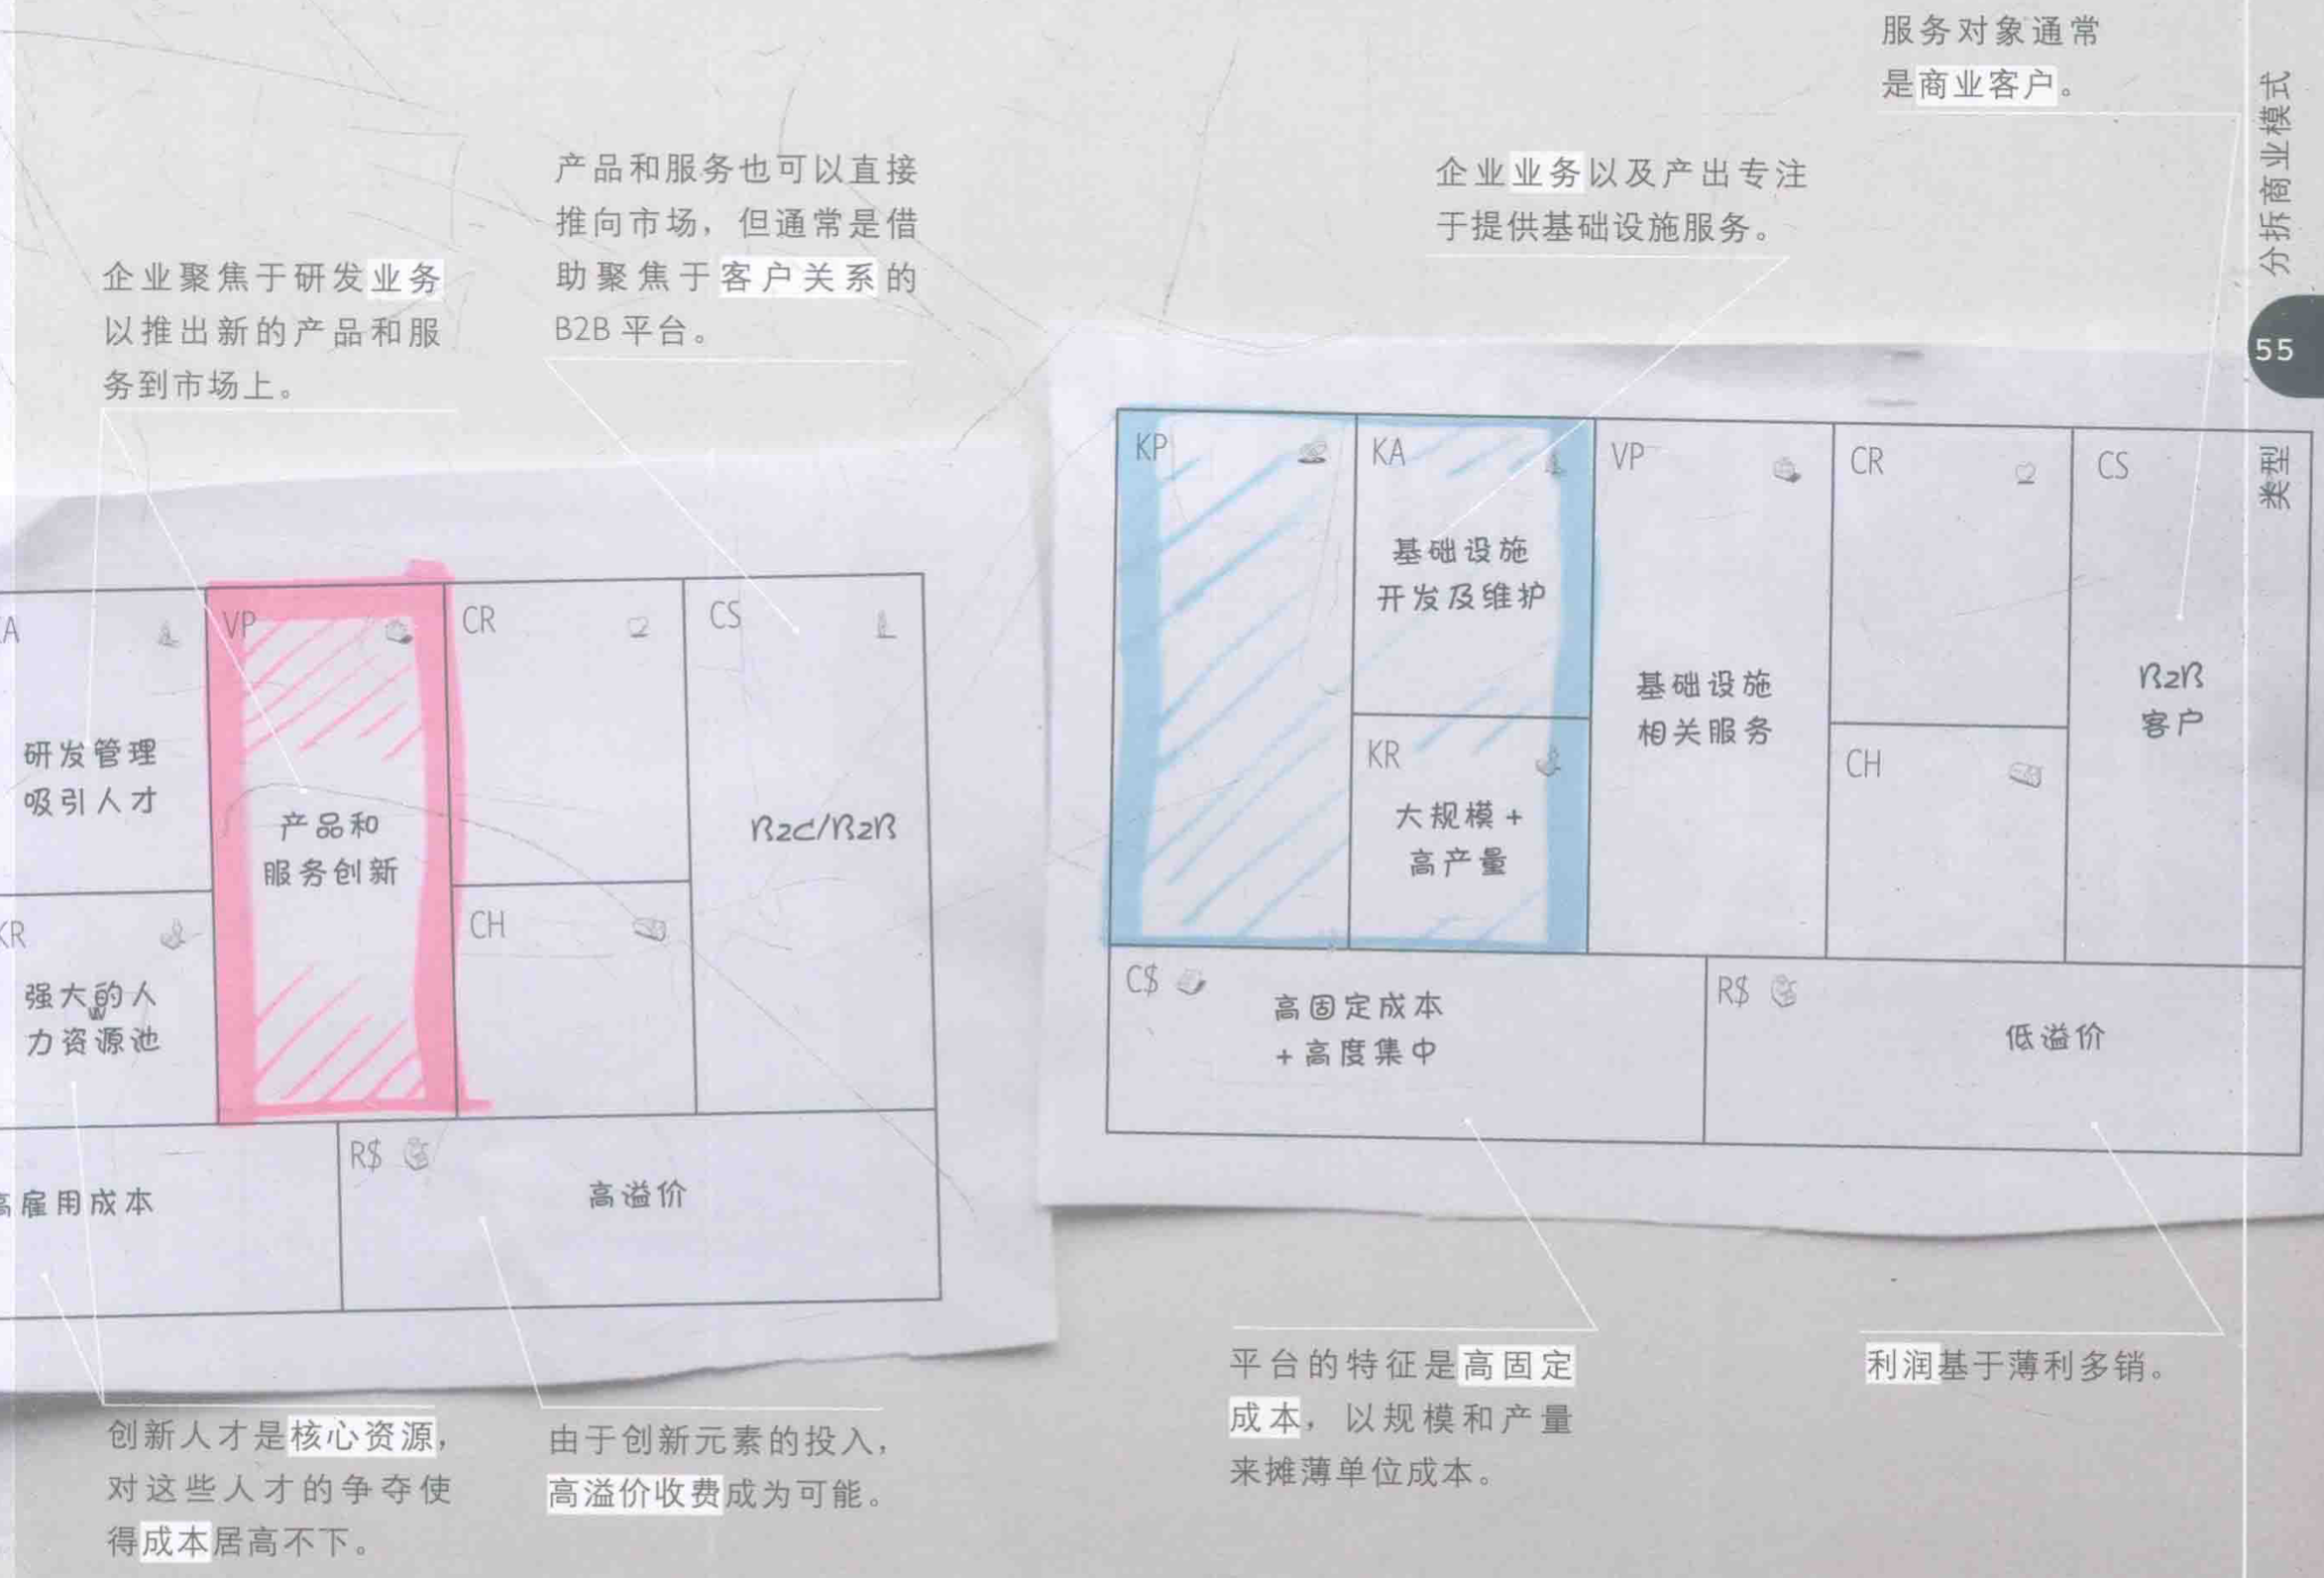
\includegraphics[width=\textwidth]{img/拆分后三个独立的商业模式2.png}
        \vspace{-0.5em}
	\end{figure}

    \subsection{长尾商业模式}
    长尾商业模式在于少量多种地销售自己的产品:它致力于提供相当多种类的小众产品,而其中的每一种卖出量相对很少。
    \begin{itemize}
        \item 将这些小众产品的销售汇总,所得收入可以像传统模式销售所得一样可观,它不同于传统模式,以销售少数的明星产品负担起绝大部分的收益。
        \item 长尾商业模式要求低库存成本以及强大的平台以保证小众商品能够及时被感兴趣的买家获得。
    \end{itemize}

    \begin{figure}[H]
		\centering
        \vspace{-0.5em}
		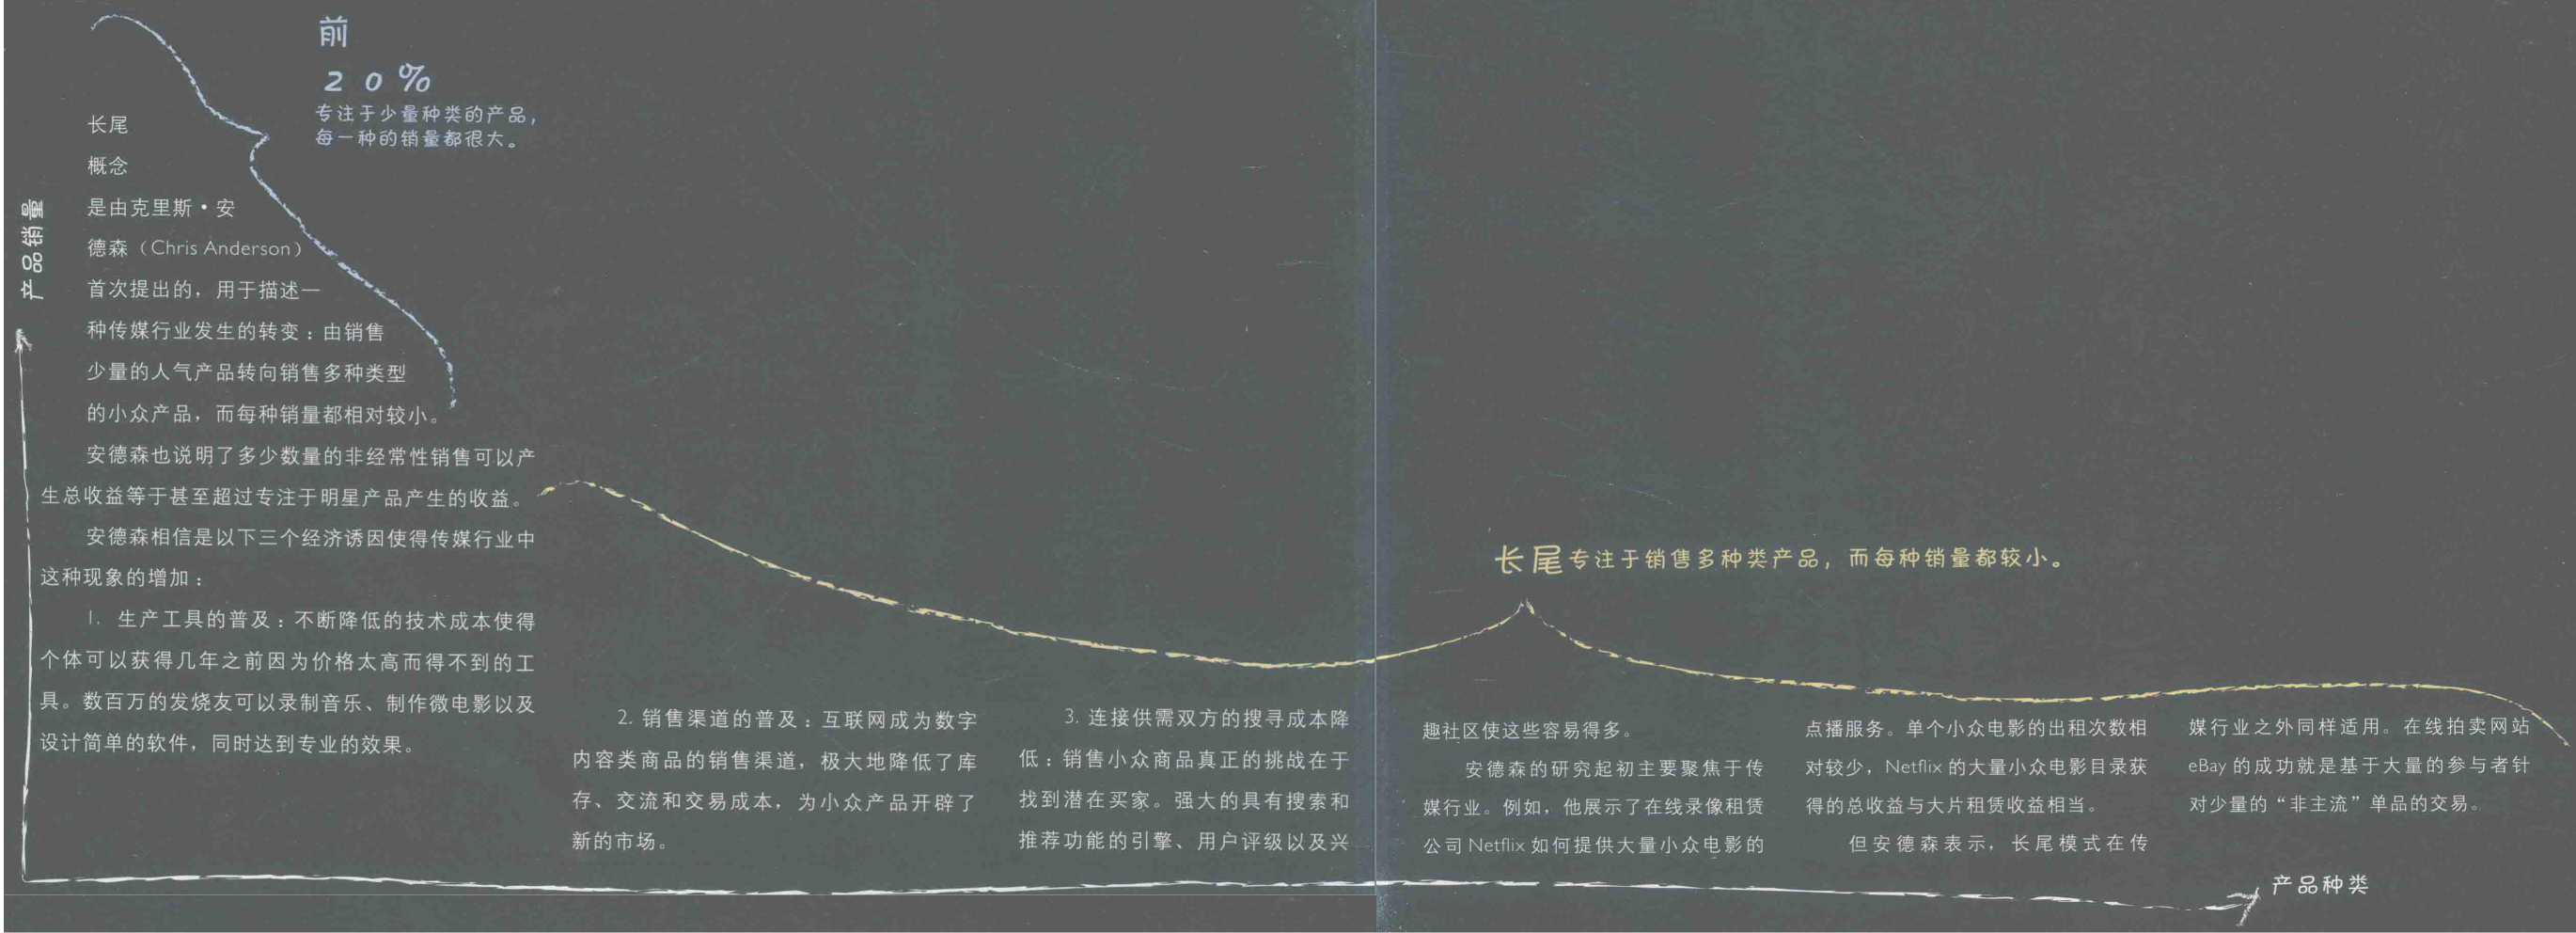
\includegraphics[width=\textwidth]{img/长尾概念的提出.png}
        \vspace{-0.5em}
	\end{figure}

    \subsubsection{图书出版行业的转型}
    \begin{figure}[H]
		\centering
        \vspace{-0.5em}
		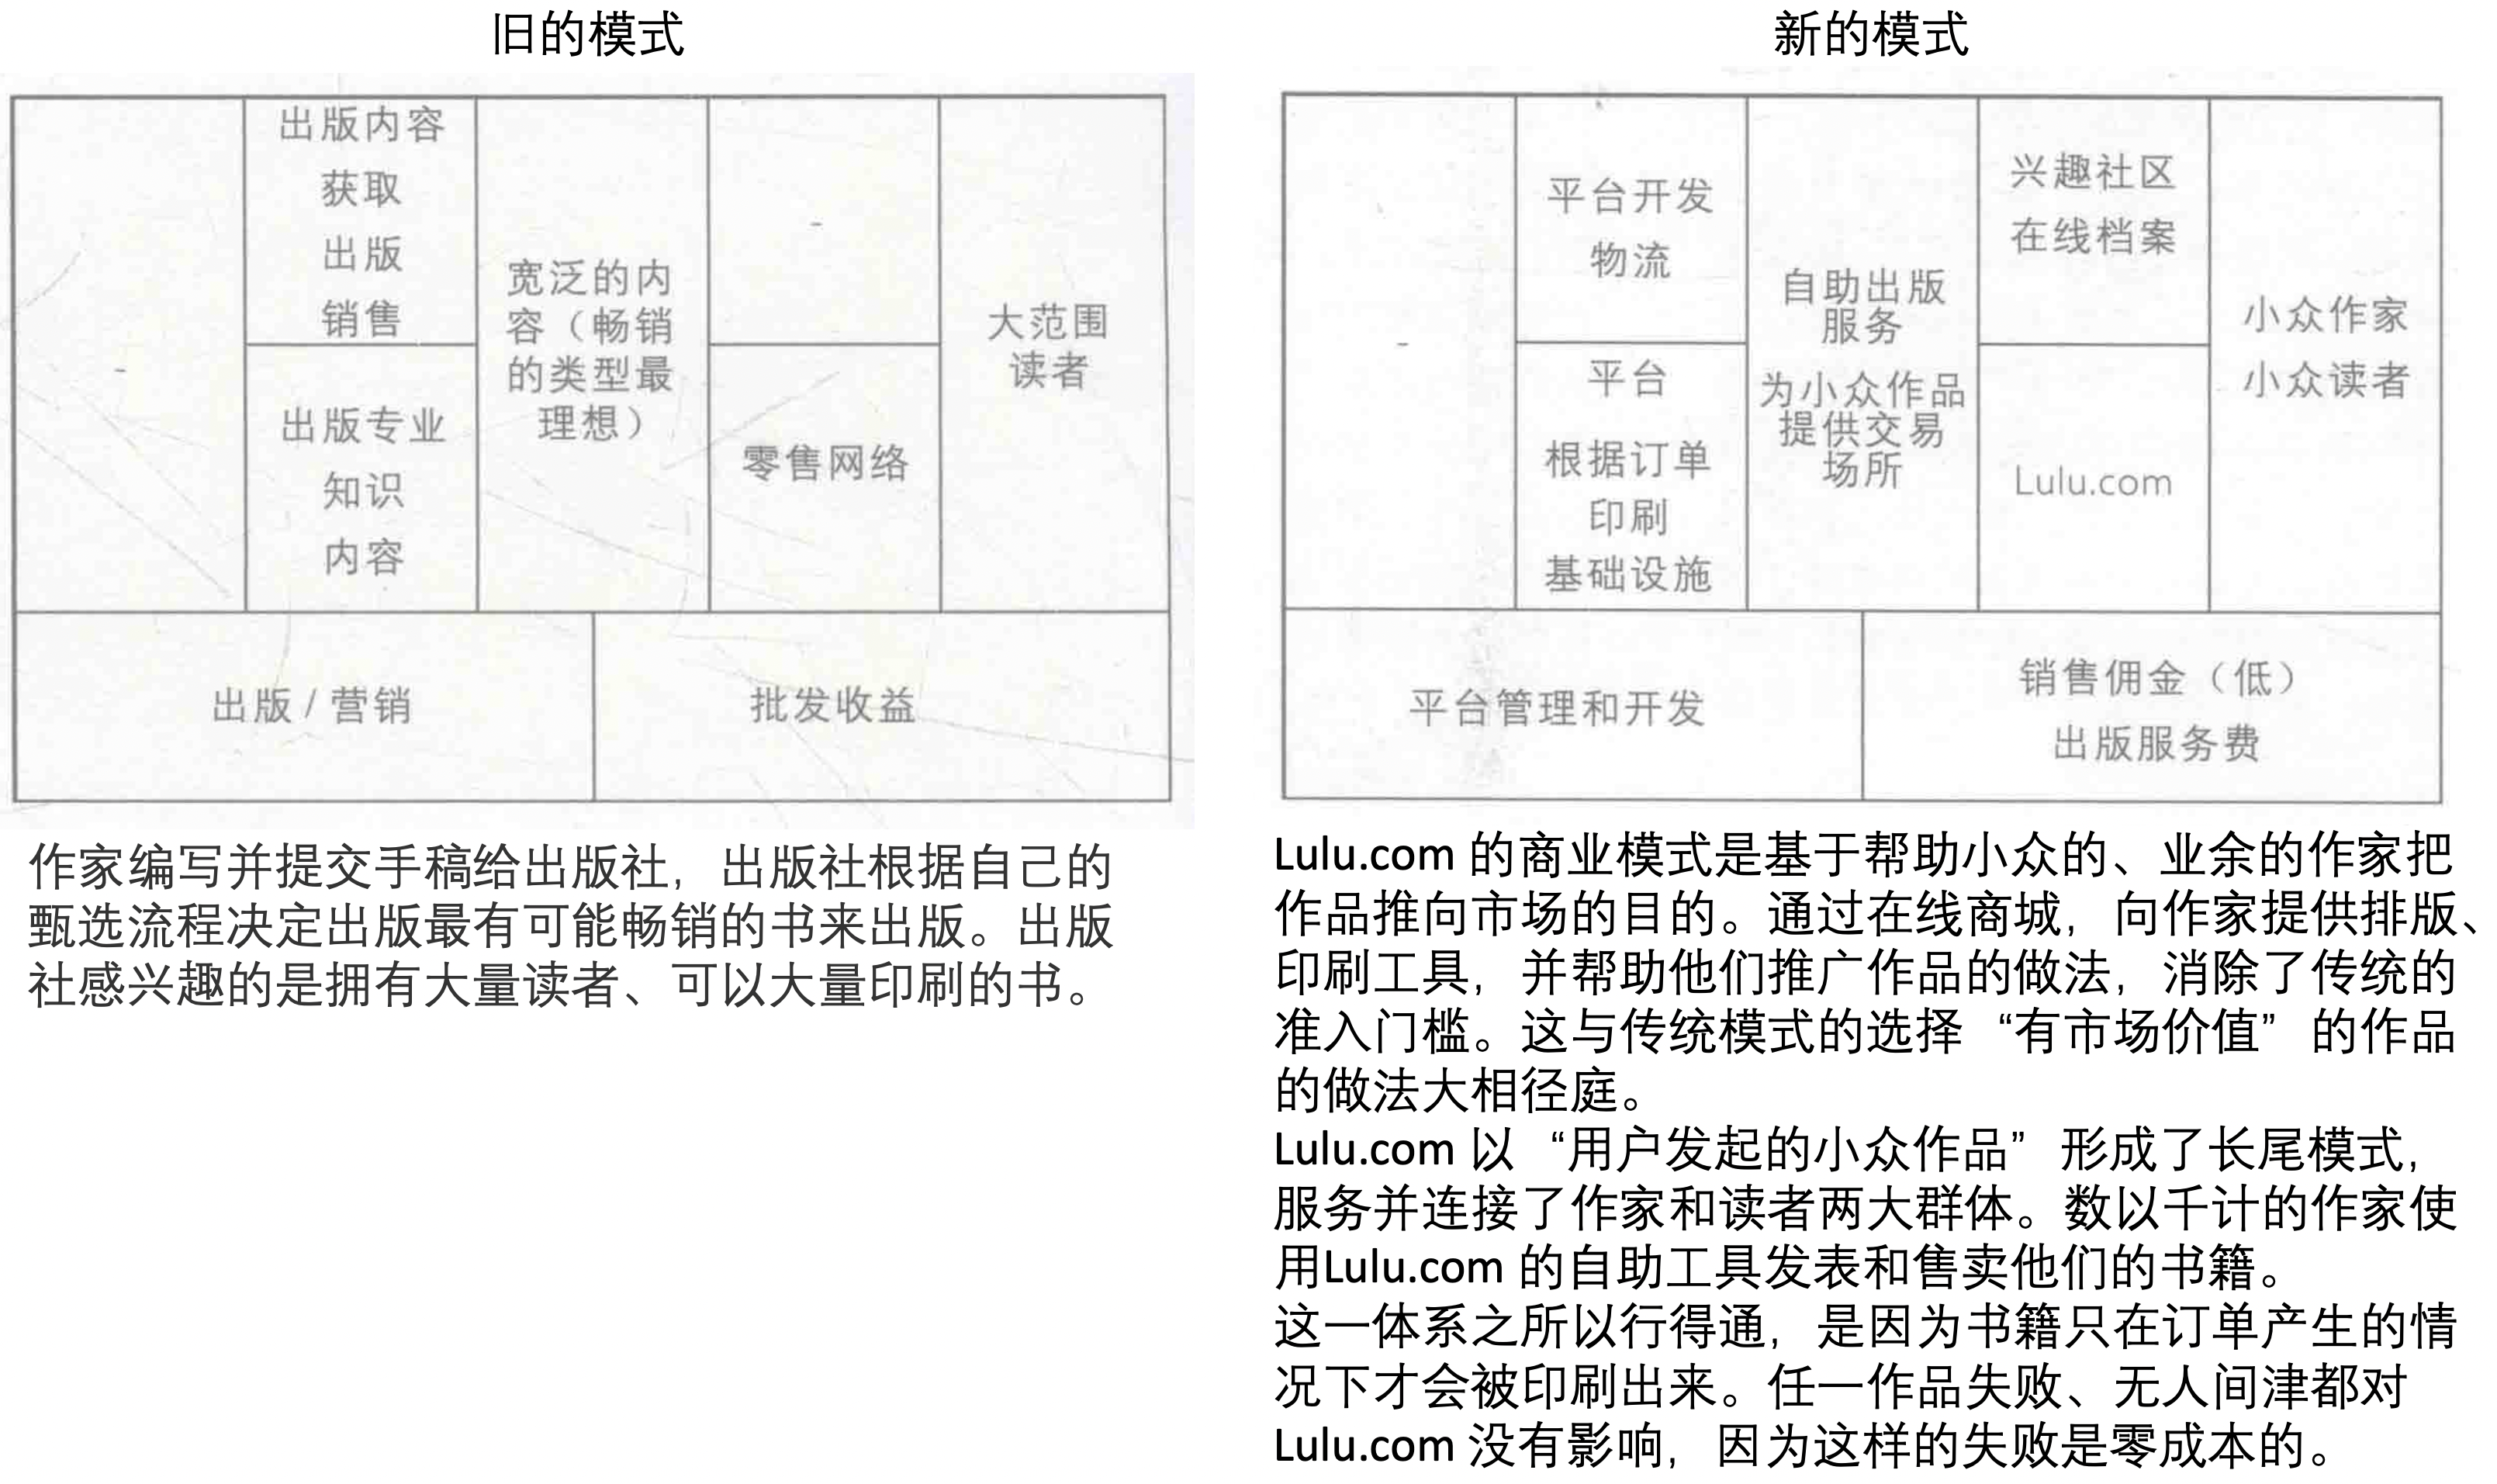
\includegraphics[width=\textwidth]{img/图书出版行业的转型.png}
        \vspace{-0.5em}
	\end{figure}

    \subsubsection{乐高的新长尾模式}
    2005年,乐高开始推出用户定制套餐——乐高工厂,允许客户使用在线设计软件,甚至允许用户选择包装盒子,让用户成为了乐高设计体验的主动参与者。
    \begin{figure}[H]
		\centering
        \vspace{-0.5em}
		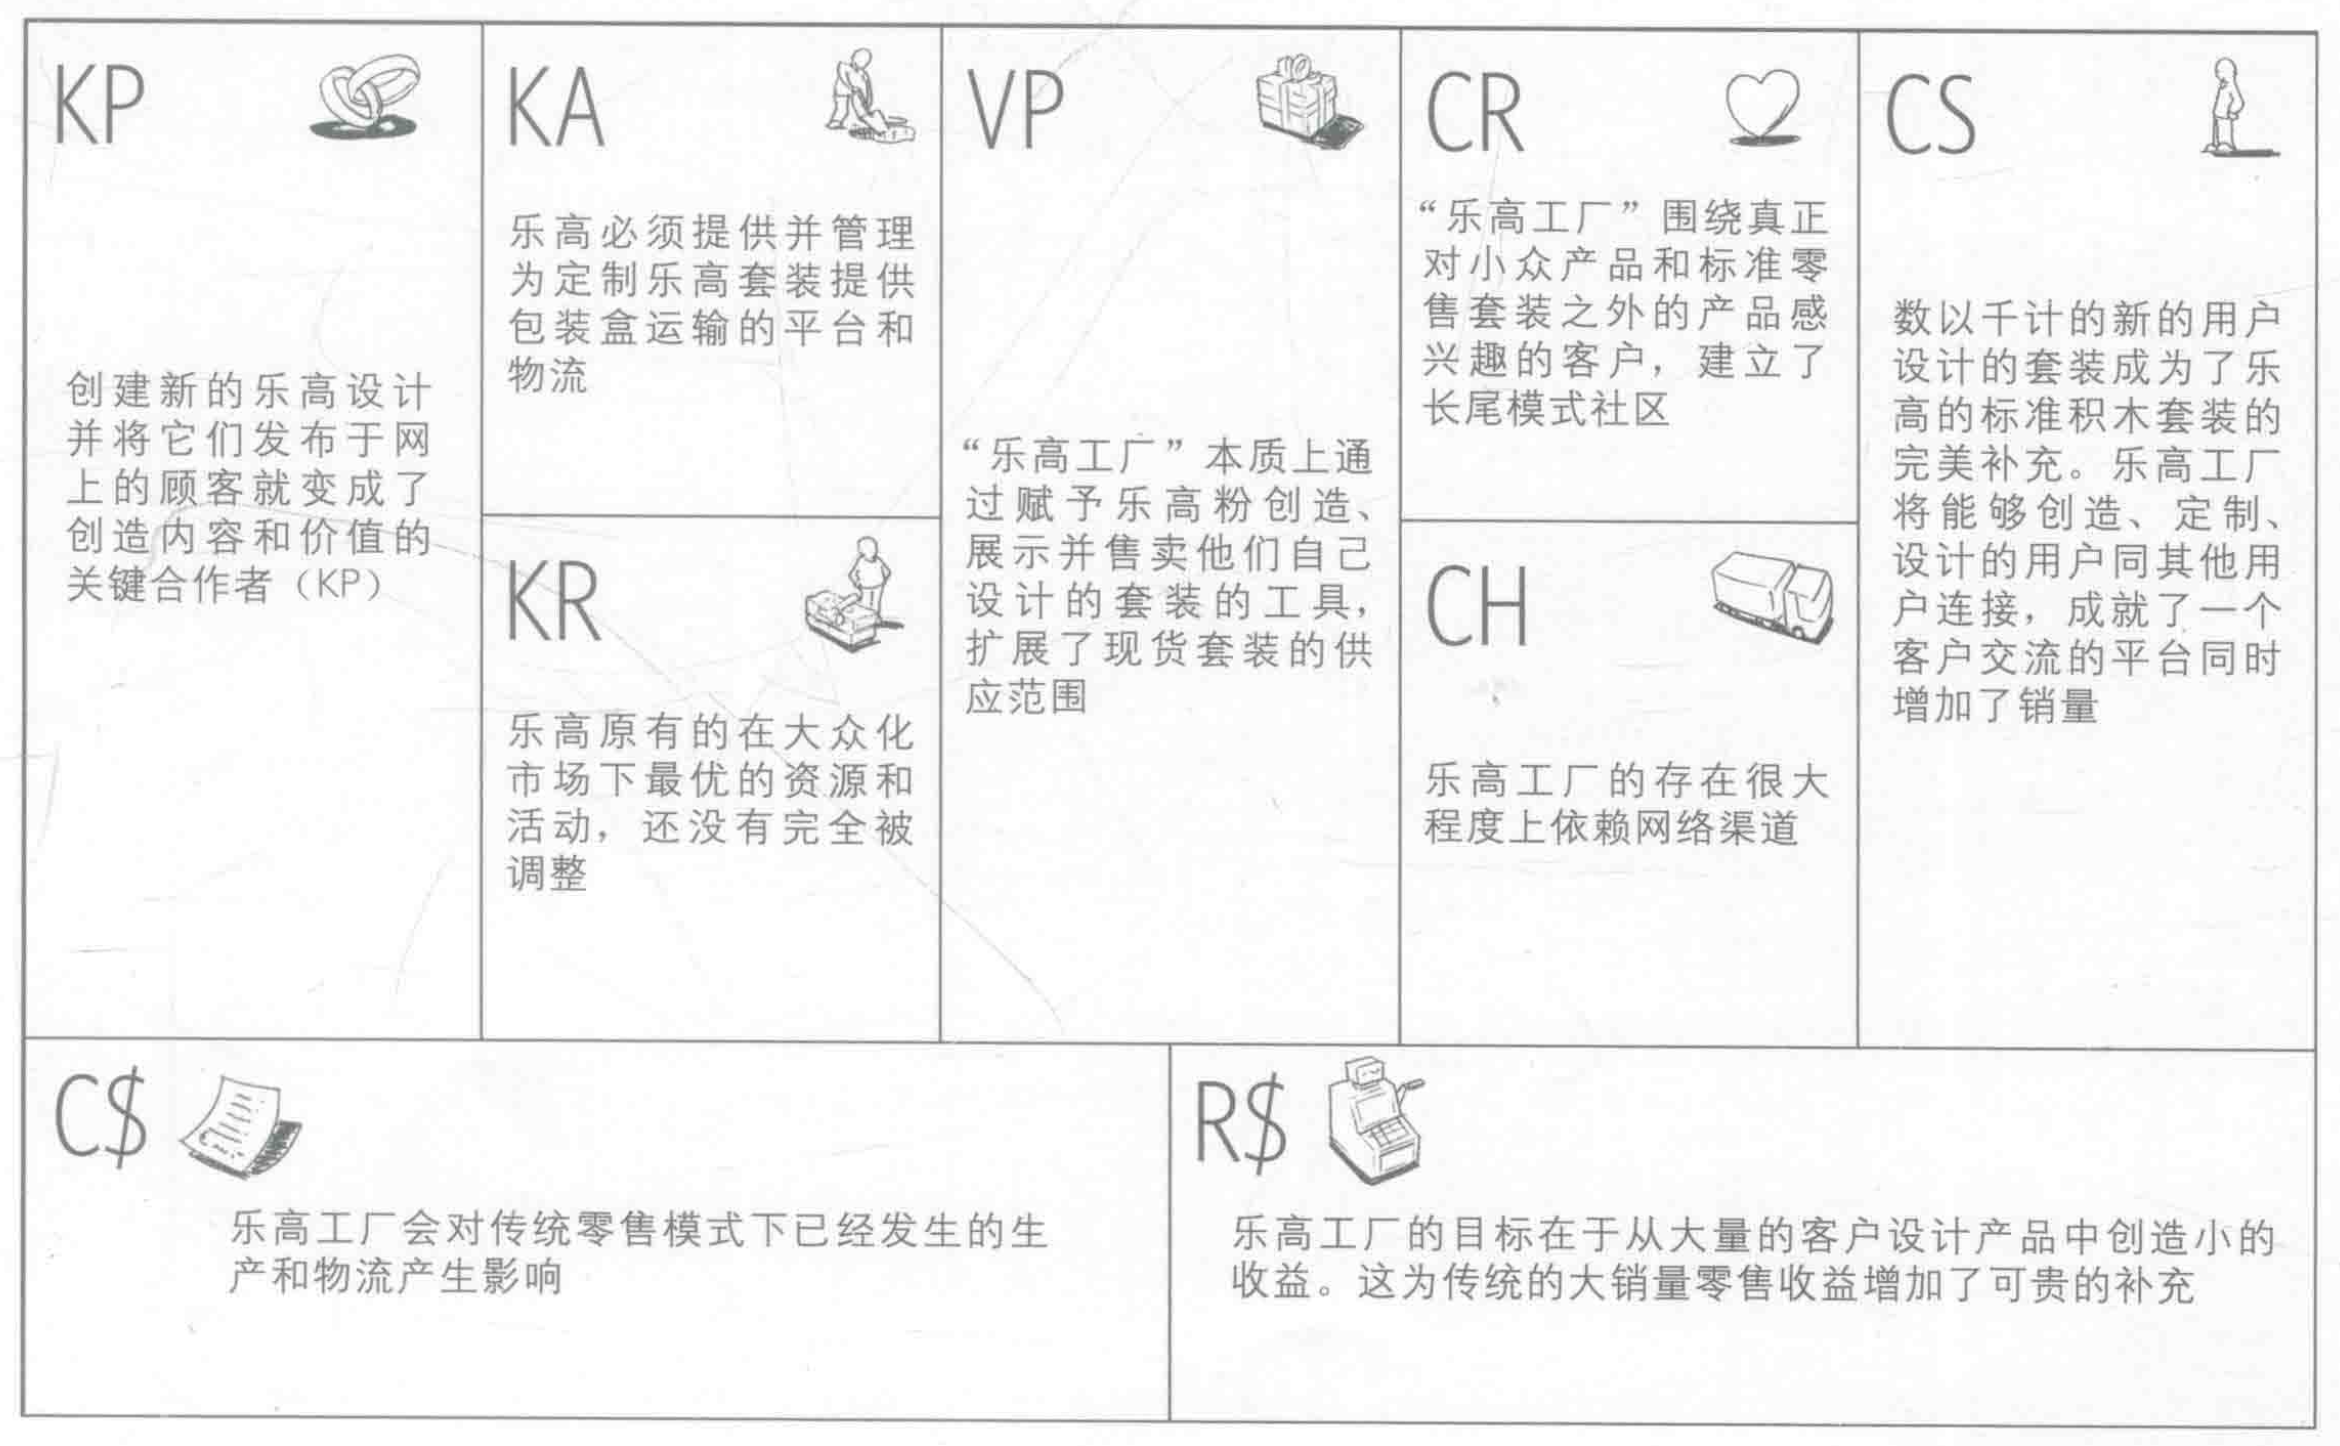
\includegraphics[width=\textwidth]{img/乐高的新长尾模式.png}
        \vspace{-0.5em}
	\end{figure}

    \subsubsection{长尾模式的流行原因与发展趋势}
    大量行业都有“长尾”的趋势
    \begin{itemize}
        \item 个人主义流行与社会物资丰富导致的需求释放
        \item 人类社会中的流行因素与趋势三年一小变、五年一大变
        \item 生产设计与渠道营销在效率上的不断提升带来的产销能力工具化、服务化
        \item 互联网技术不断发展导致的供需双方匹配更加便利
        \item 复用生产和渠道,可以和热销品并存(长尾模式背后往往有大公司的影子)
    \end{itemize}

    长尾模式的共性与发展趋势
    \begin{itemize}
        \item 对生产环节(含渠道)的标准化程度要求较高(媒体、影视、游戏、一般日用品)
        \item 生产设计环节一般仍依赖于大型厂家,渠道依赖互联网(社区也可能是创意、构思的来源)
        \item “长尾之后”:突破因传统生产、设计、营销导致的二八曲线,长尾部分扁平化;形成若干“小众中心”,并分别向“大众中心”转化
    \end{itemize}

    \begin{figure}[H]
		\centering
        \vspace{-0.5em}
		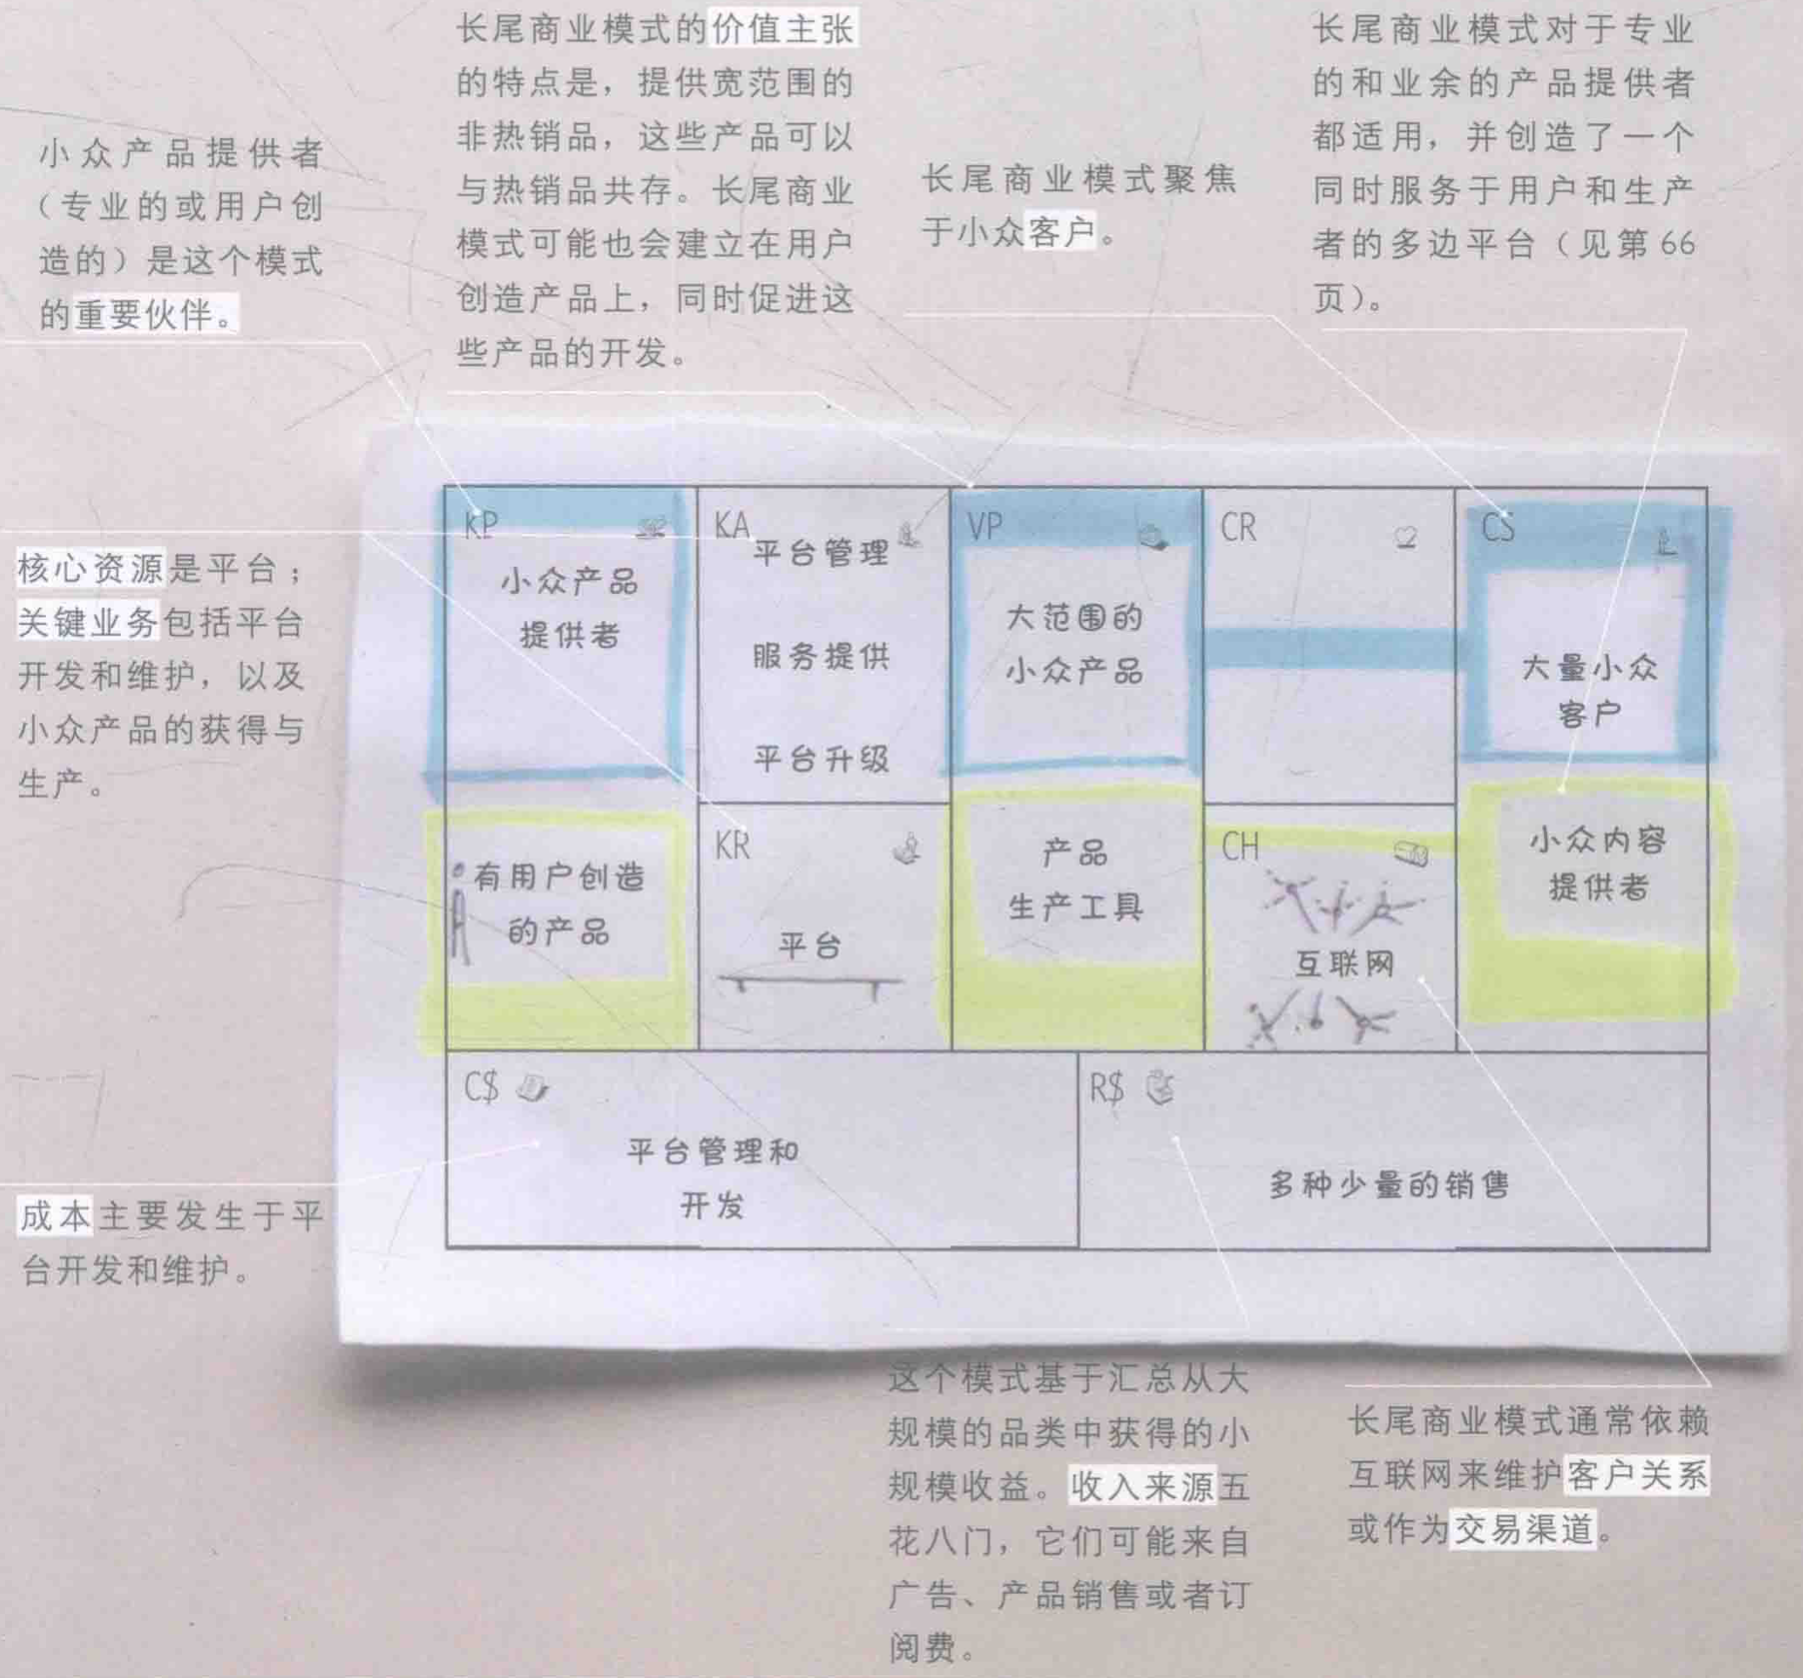
\includegraphics[width=0.85\textwidth]{img/长尾模式总结.png}
        \vspace{-0.5em}
	\end{figure}

    \subsection{多边平台商业模式}
    多边平台(多边市场)是将两个或更多独立但相互依存的客户群体连接在一起的平台。
    \begin{itemize}
        \item 这样的平台对于平台中某一群体的价值在于平台中其他客户群体的存在。平台通过促进不同群体间的互动而创造价值,例如信用卡将商家和持卡人连接。
        \item 多边平台的价值提升在于它所吸引的用户数量的增加,这种现象被称为网络效应。
        \item 平台对于单个用户群体的价值本质上取决于平台中“另一群体”的用户数量,例如游戏开发商之所以会为某一个电子游戏设备开发新游戏是因为已经有大量的玩家在使用它。
        \item 多边平台经常会面临一个“先有鸡还是先有蛋”的两难困境。
        \begin{itemize}
            \item 解决这一问题的一种方式是向某一个客户群体发放补贴
            \item 平台需要使用低廉或免费的价值主张来吸引某一个群体加入平台,需要明确群体加入平台的目的,以及哪一边是需要给予补贴
        \end{itemize}
    \end{itemize}

    \subsubsection{谷歌的商业模式}
    \begin{itemize}
        \item 谷歌商业模式的核心就是其价值主张:在全球网络中发布精准定位的文字广告
        \item 谷歌的收益模式:
        \begin{itemize}
            \item 从广告商群体中赚钱,对另外两个客户群体(上网浏览者和内容提供者)给予补贴
            \item 广告浏览次数越多,广告商赚取的收益越多;广告商赚取的利益越多,越多的第三方网站和AdSense合作
            \item 广告商在第三方网站上与广告关键词相关的搜索词条或者搜索内容竞价。通过AdWords,越热门的关键词竞价成功就需要付出越高的价格
        \end{itemize}
        \item 谷歌的核心资源:搜索平台,基于一套具有搜索和配对功能的高度复杂的专利算法,配合强大的IT硬件支持,有以下三项服务
        \begin{itemize}
            \item 网络搜索(Google.com)
            \item 广告(AdWords):允许广告商可以发布广告并将链接放置到谷歌的搜索界面中,用户进入搜索引擎进行搜索的时候,谷歌也会显示相关的广告,使得针对性进一步提高
            \item 第三方内容变现服务(AdSense):自动分析第三方网站内容并为浏览者提供内容相关的文字和图像广告,谷歌从广告收益中分得一部分
        \end{itemize}
        \item 谷歌的关键业务
        \begin{itemize}
            \item 建立并维护搜索引擎的基础设施
            \item 三项主要功能的管理
            \item 将平台推广给新用户、新的内容提供商和新的广告合作商
        \end{itemize}
    \end{itemize}

    \begin{figure}[H]
		\centering
        \vspace{-0.5em}
		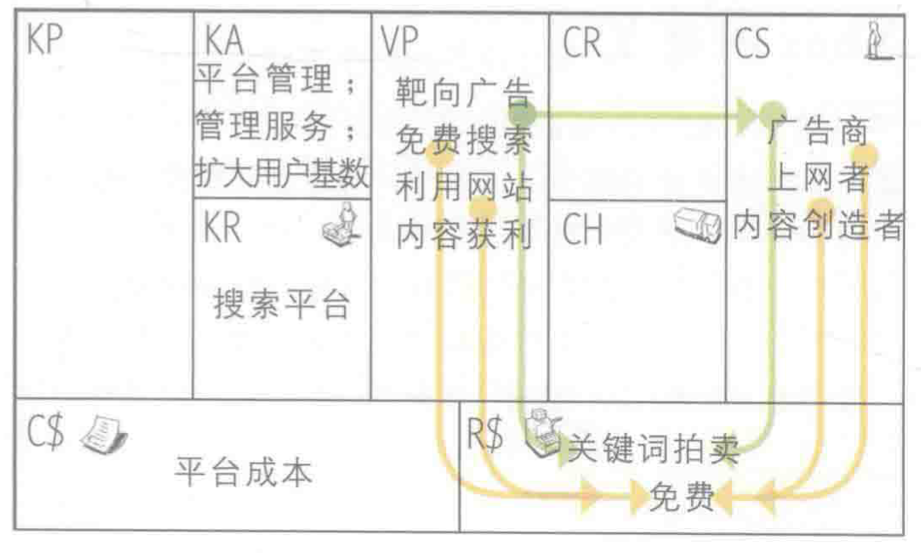
\includegraphics[width=0.65\textwidth]{img/谷歌的商业模式.png}
        \vspace{-0.5em}
	\end{figure}

    \subsubsection{苹果公司的平台运营商进化记}

    \begin{figure}[H]
		\centering
        \vspace{-0.5em}
		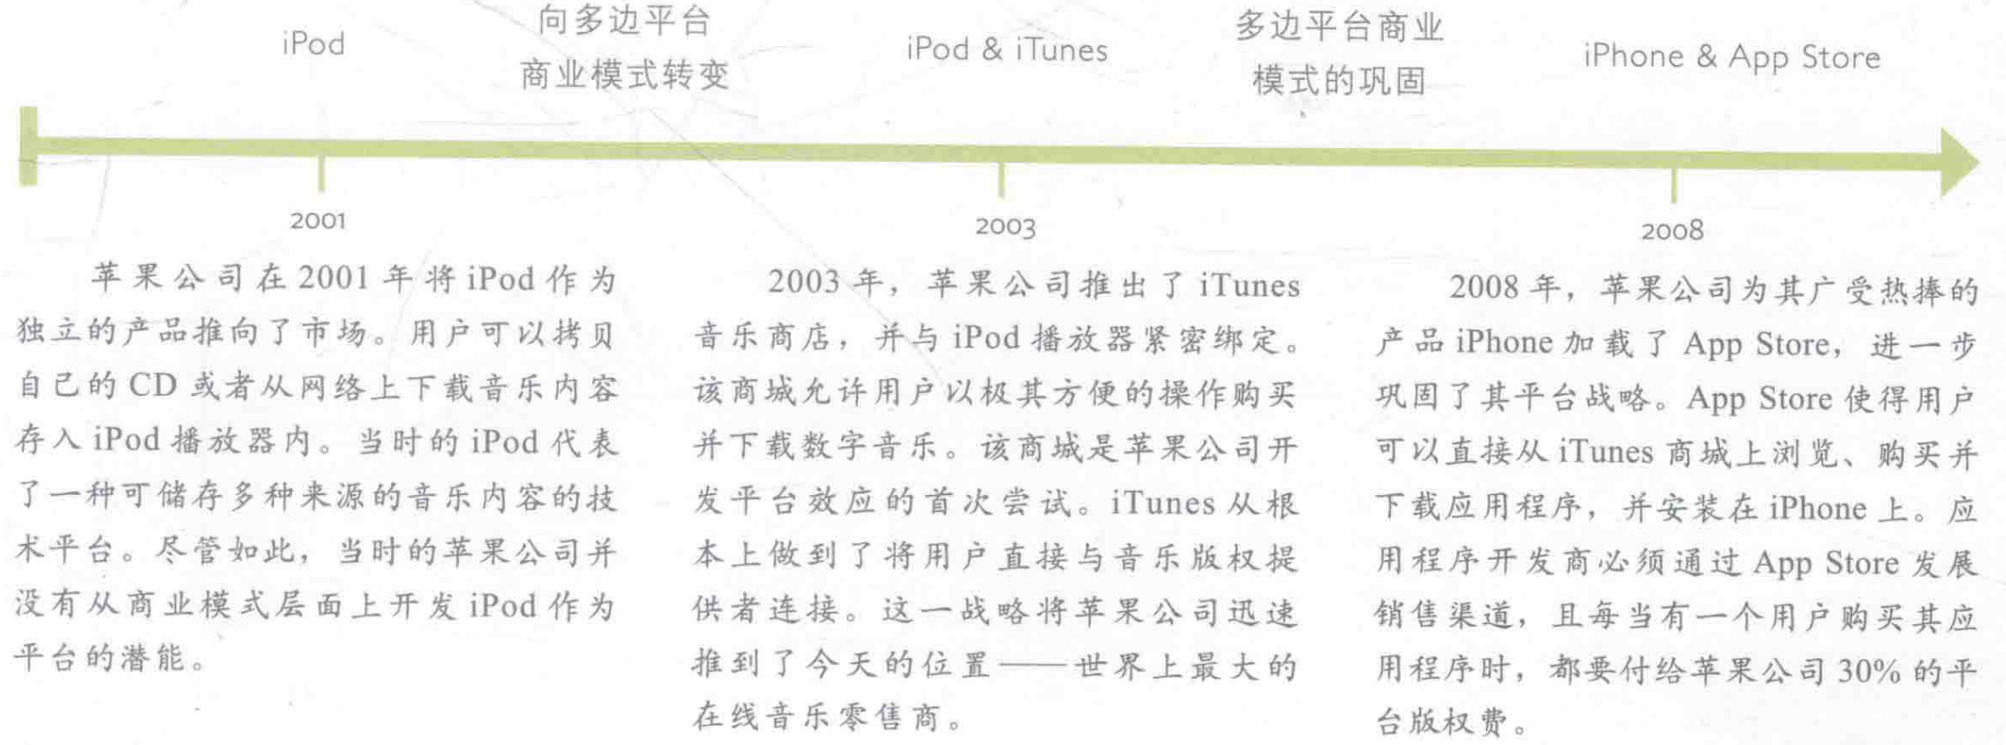
\includegraphics[width=0.95\textwidth]{img/苹果公司的平台运营商进化记.png}
        \vspace{-0.5em}
	\end{figure}

    \subsubsection{多边平台商业模式总结}

    \begin{figure}[H]
		\centering
        \vspace{-0.5em}
		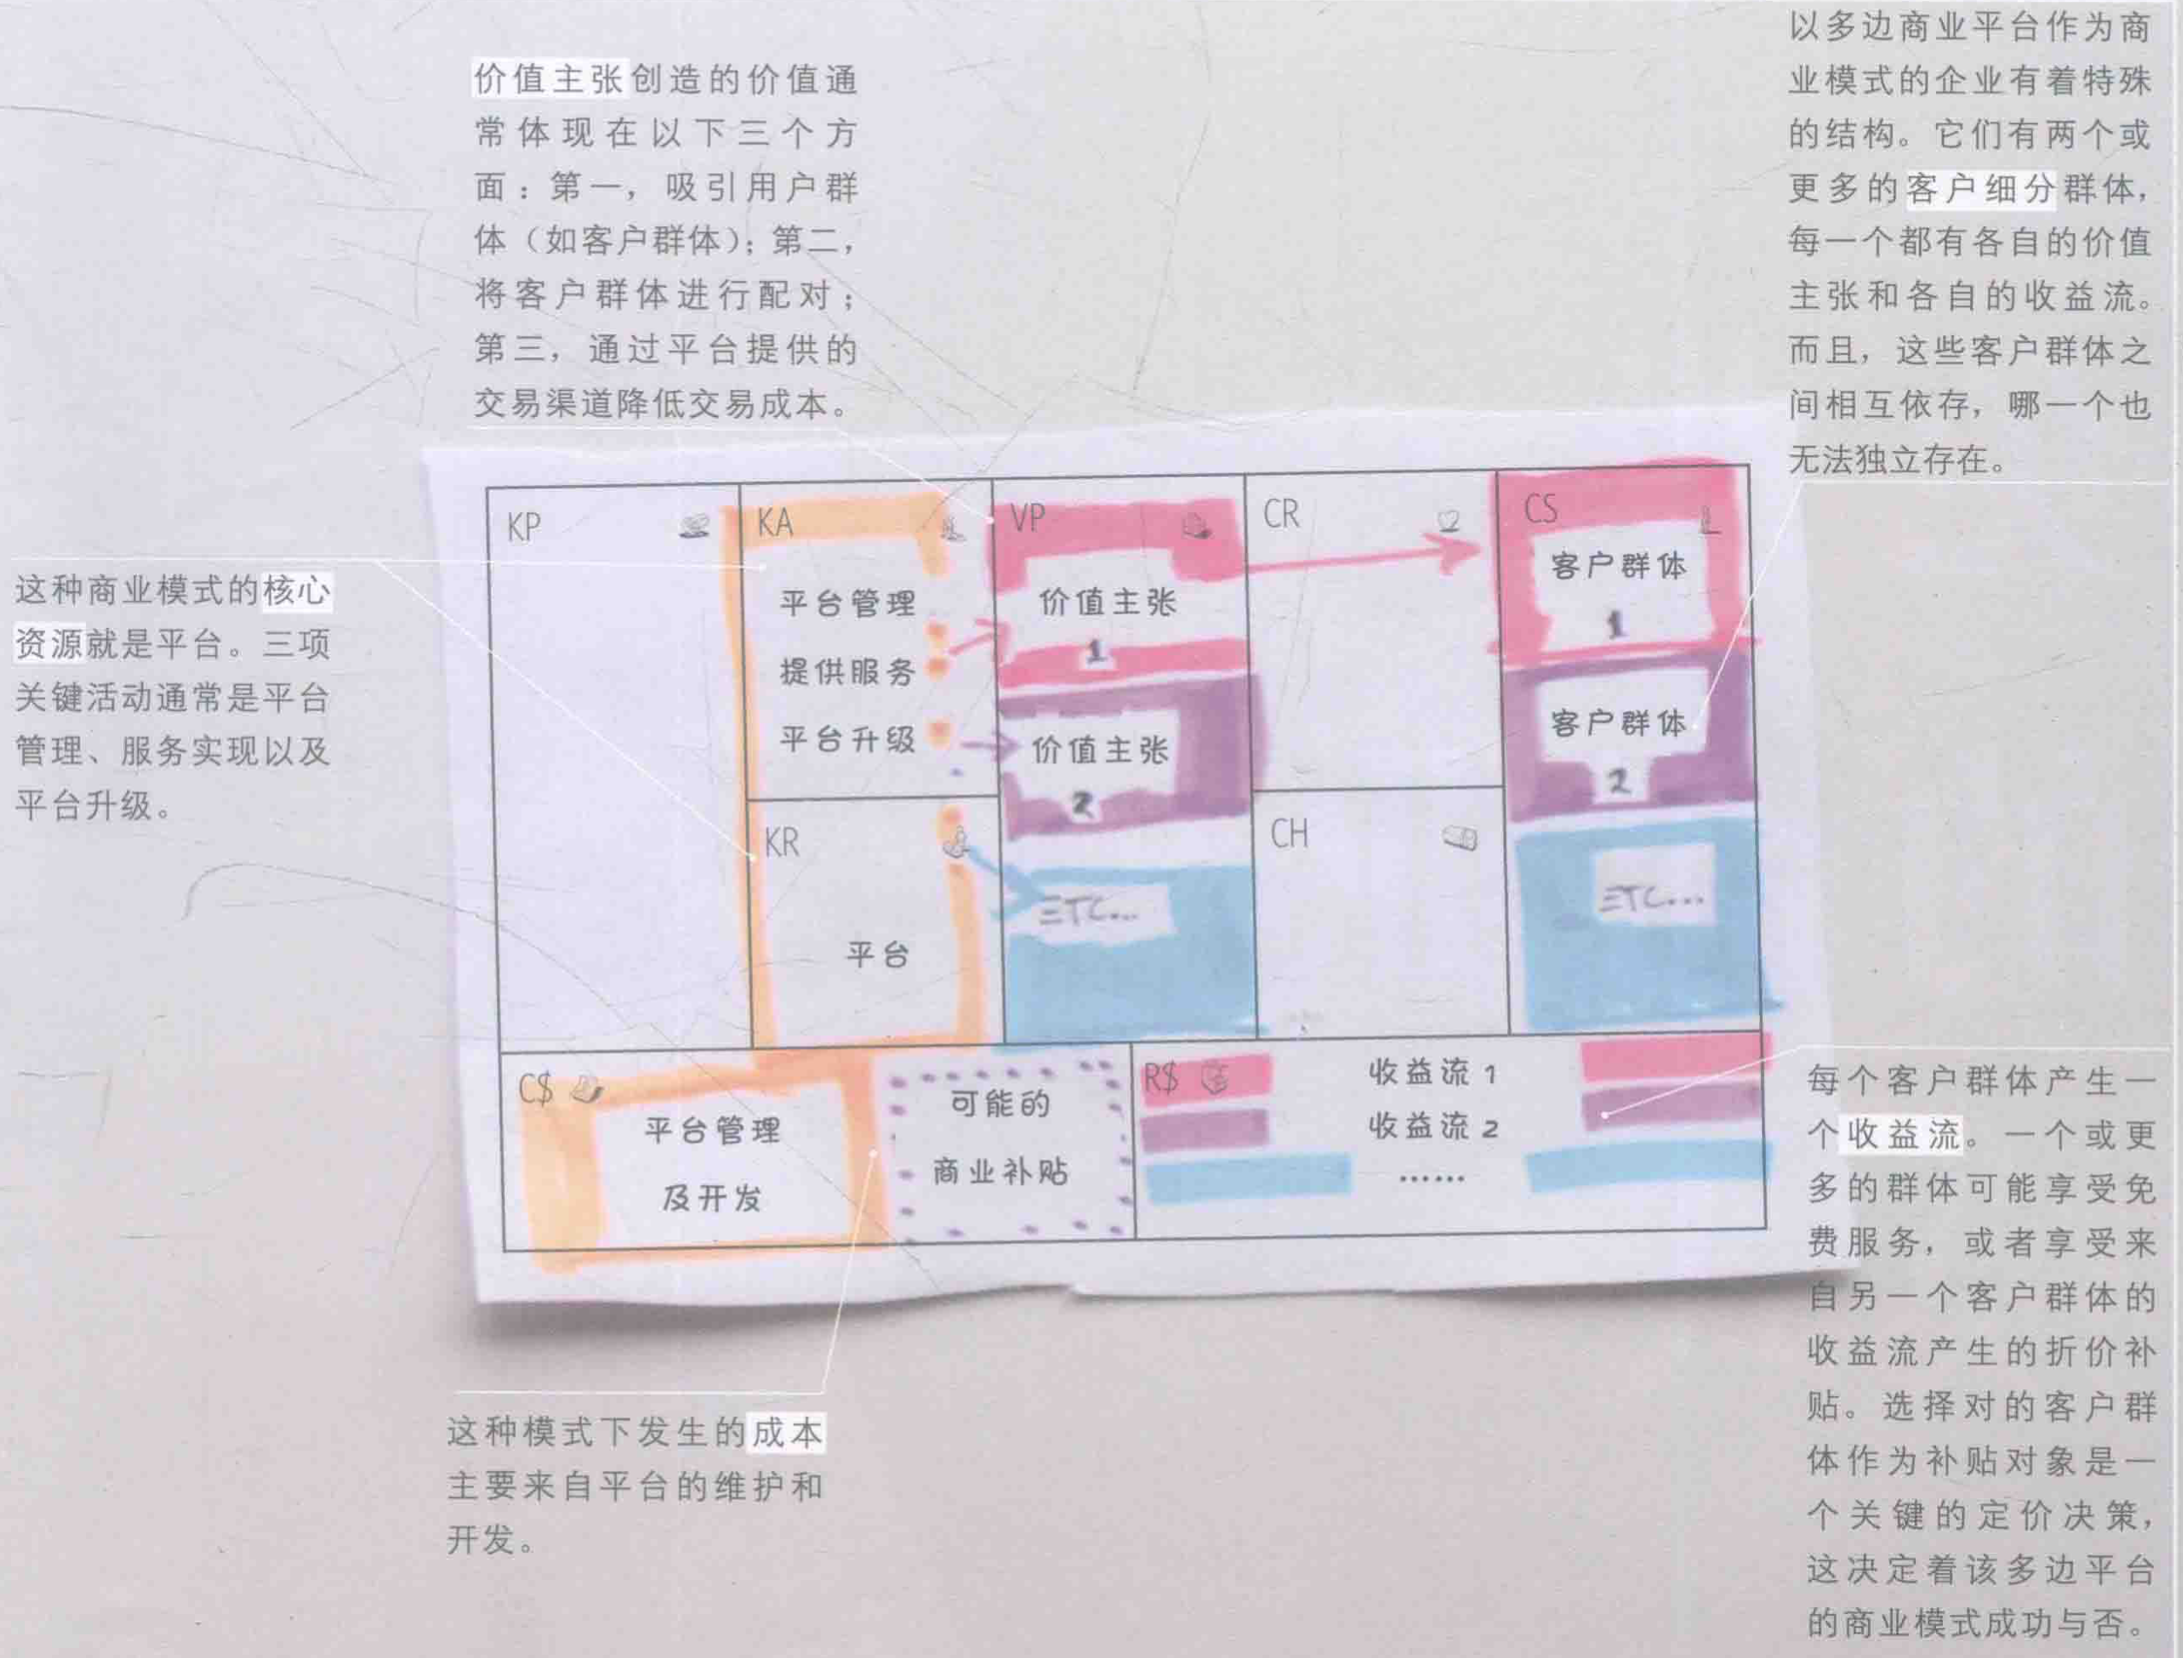
\includegraphics[width=0.95\textwidth]{img/多边平台商业模式总结.png}
        \vspace{-0.5em}
	\end{figure}

    \subsection{免费商业模式}
    在免费商业模式中,至少有一个关键的客户群体是可以持续免费地享受服务
    \begin{itemize}
        \item 不付费的客户所得到的财务支持来自商业模式中的另一个客户群体。
        \item 任何价格为0的产品产生的需求要数倍于价格为1分钱或者其他定价的商品产生的需求。
        \item 数字产品与服务的复制传播成本接近于0,海量用户下边界成本也趋向于0
        \item 三种可行的免费商业模式:
        \begin{itemize}
            \item 广告模式:基于多边平台的免费商品
            \item 免费增值:免费的基本服务,可选的增值服务
            \item 钓鱼模式:以免费或很便宜的初始价格吸引客户,并引导其重复购买
        \end{itemize}
    \end{itemize}

    \subsubsection{广告:一个多边平台商业模式}
    广告是一种实现免费供给的、成熟的收益来源

    这种模式中一个让人印象深刻的例子就是Metro,其天才之处在于改变了传统日报的发行模式
    \begin{itemize}
        \item 它的报纸是免费提供的,派发以在人流密集的办公区以及公共交通网点人工发放或陈列在展架上供行人自取
        \item 它的报纸编辑质量只需要满足年轻的上班族通勤往返途中消磨时间用即可,这就削减了报纸的编辑成本 
    \end{itemize}

    \begin{figure}[H]
		\centering
        \vspace{-0.5em}
		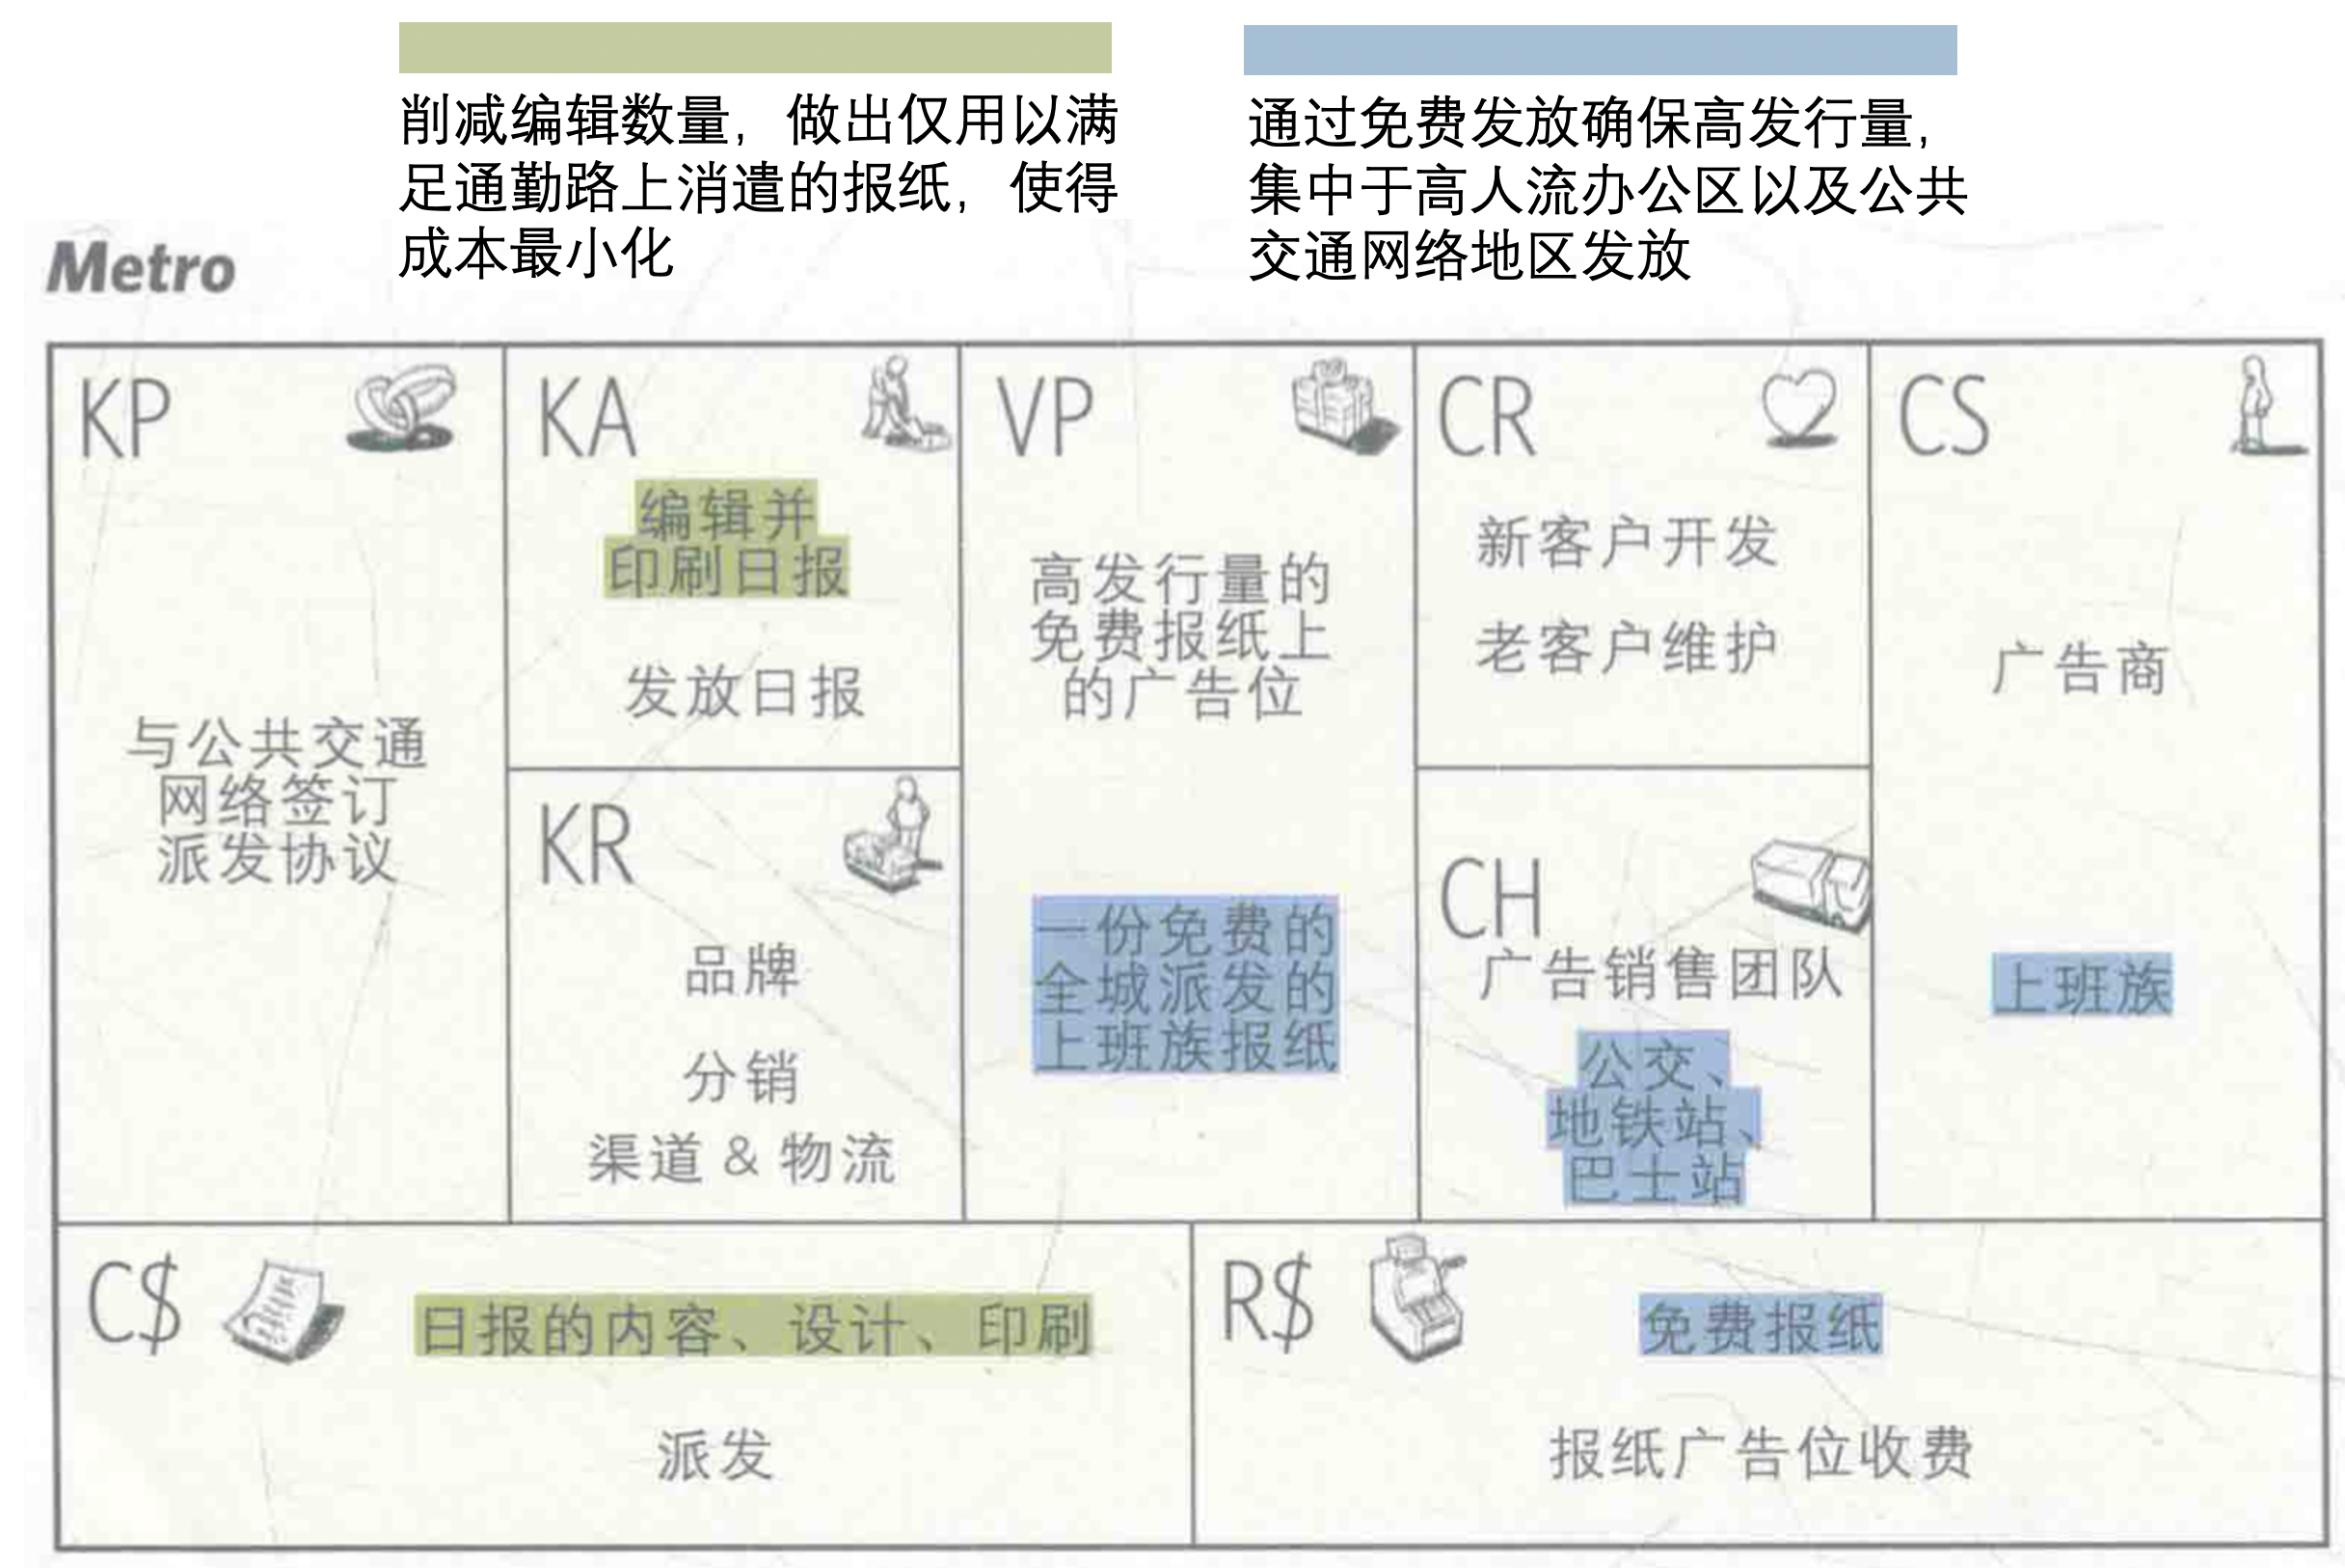
\includegraphics[width=0.7\textwidth]{img/Metro的商业模式.png}
        \vspace{-0.5em}
	\end{figure}

    \begin{figure}[H]
		\centering
        \vspace{-0.5em}
		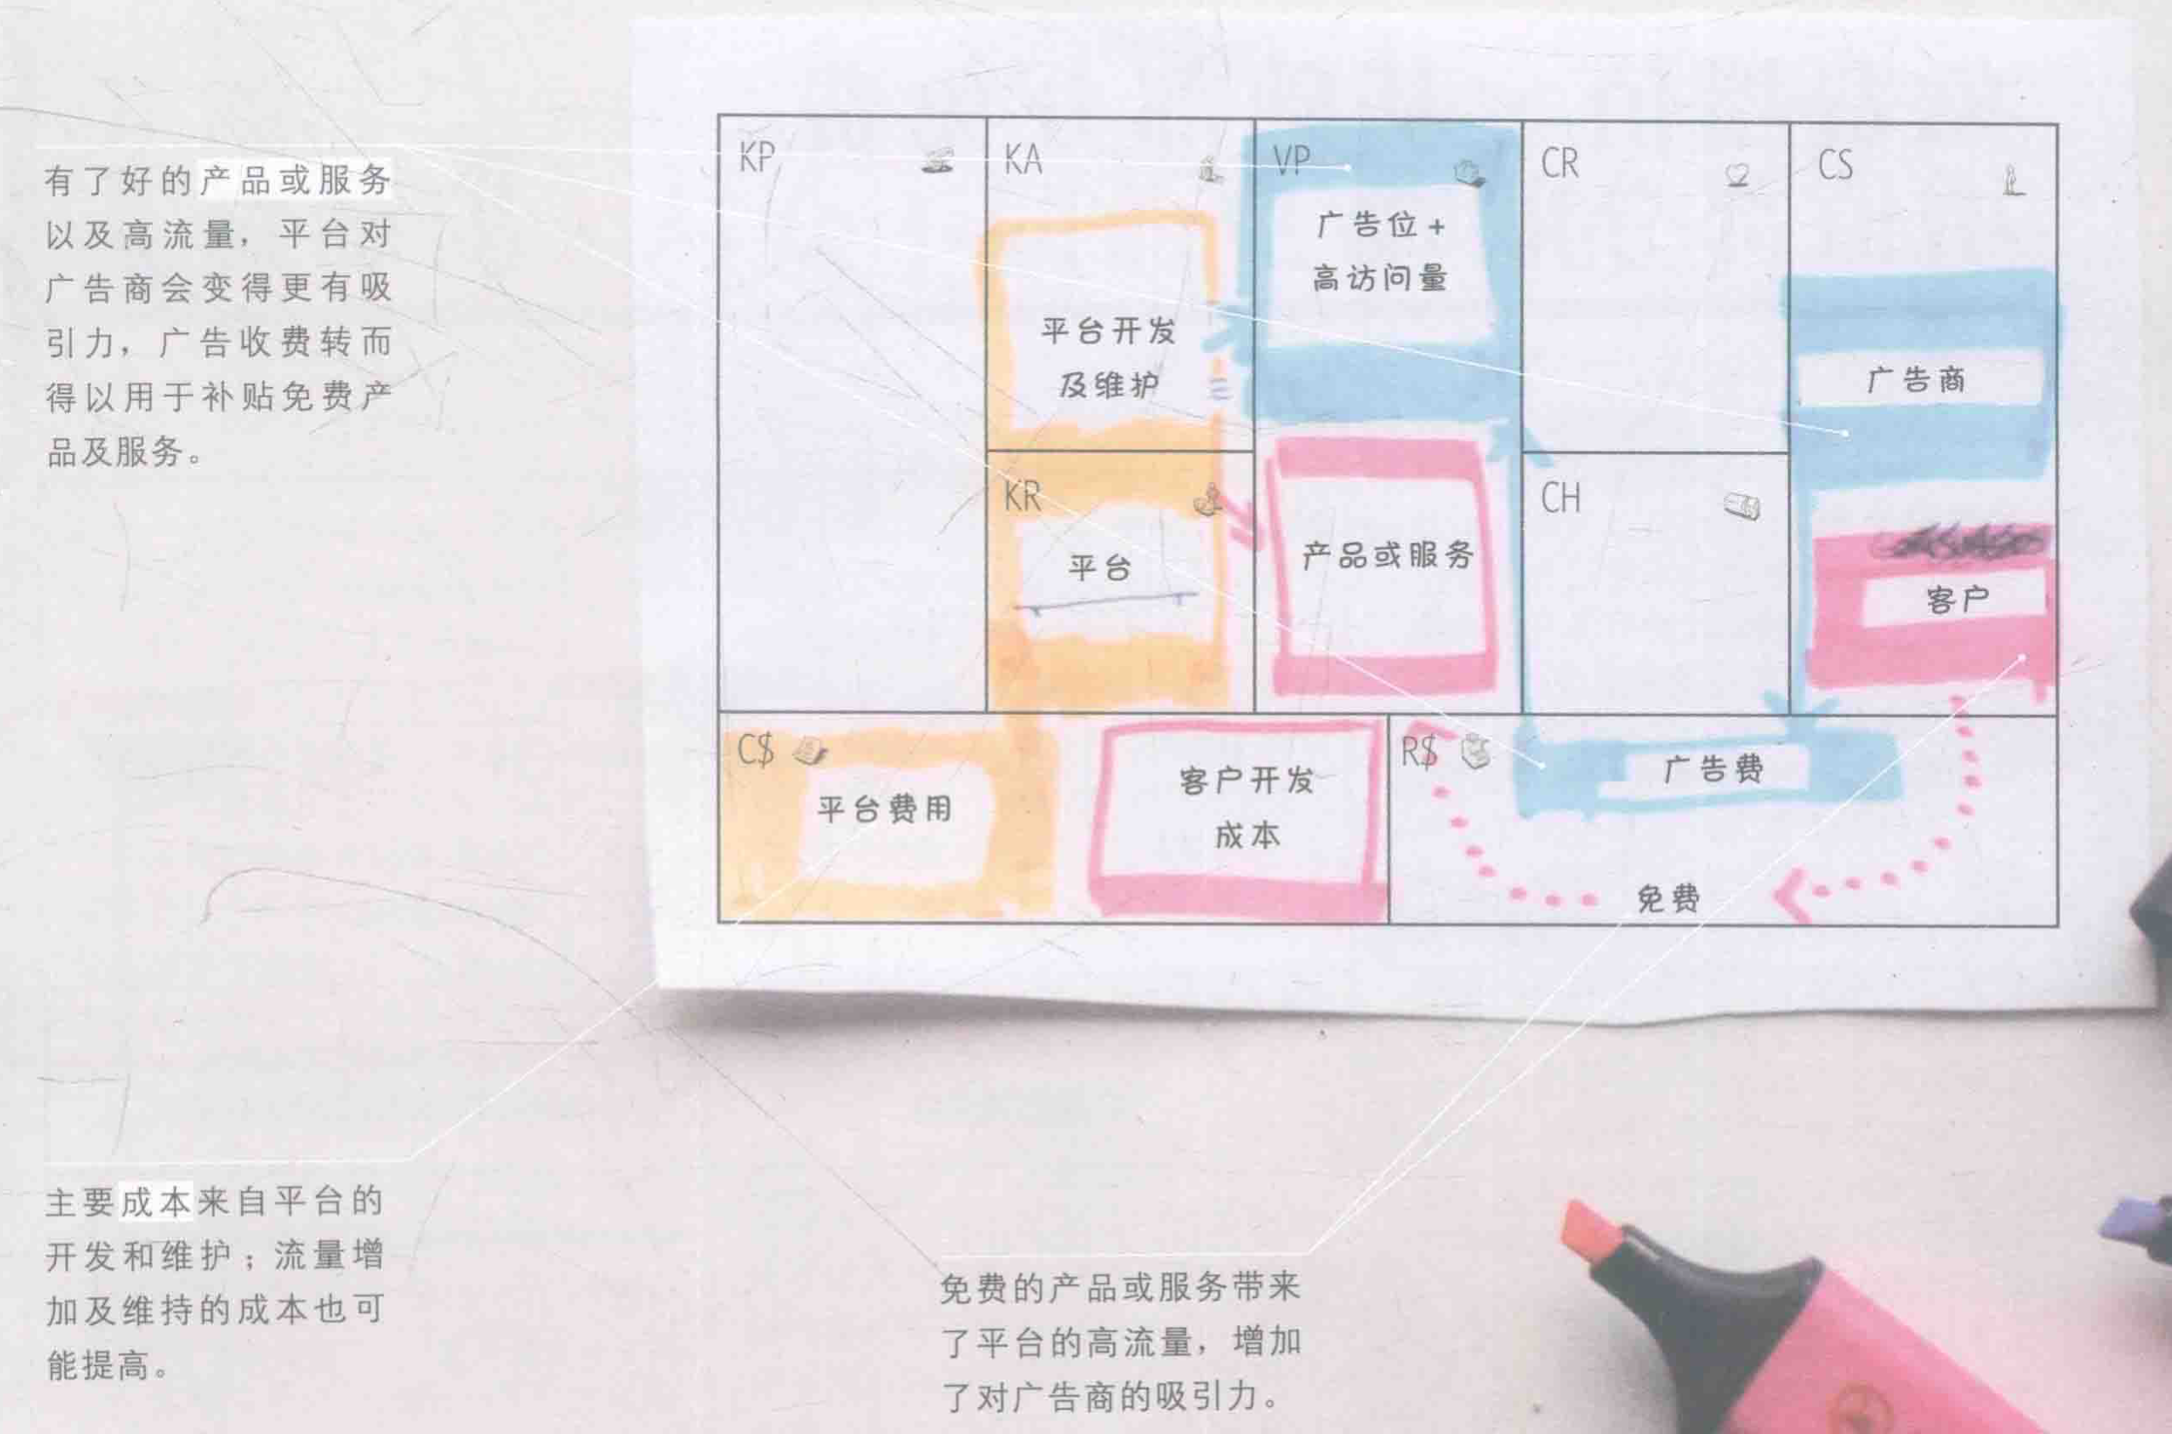
\includegraphics[width=0.8\textwidth]{img/广告:一个多边平台商业模式.png}
        \vspace{-0.5em}
	\end{figure}

    \subsubsection{免费增值:基础部分免费,增值部分收费}
    基于网络将免费的基础服务与付费的增值服务相结合,大量用户从免费服务获益,少量用户为增值服务付费
    \begin{itemize}
        \item 不到10\%的用户会为增值服务付费
        \item 两个关键指标:关注免费用户服务成本(低边界成本)与增值用户转化率
    \end{itemize}

    \paragraph{照片分享网站Flickr}~{}

    Flickr的用户可以免费获得一个基本账户,使得他们得以上传和分享照片。
    \begin{itemize}
        \item 免费服务有一些限制条件,例如有限存储空间以及每月可上传的图片数量有限
        \item 但支付少量的年费,用户就可以买到一个“专业”账户,并享受无限量的上传数量和存储空间,以及一些额外功能
    \end{itemize}
    \begin{figure}[H]
		\centering
        \vspace{-0.5em}
		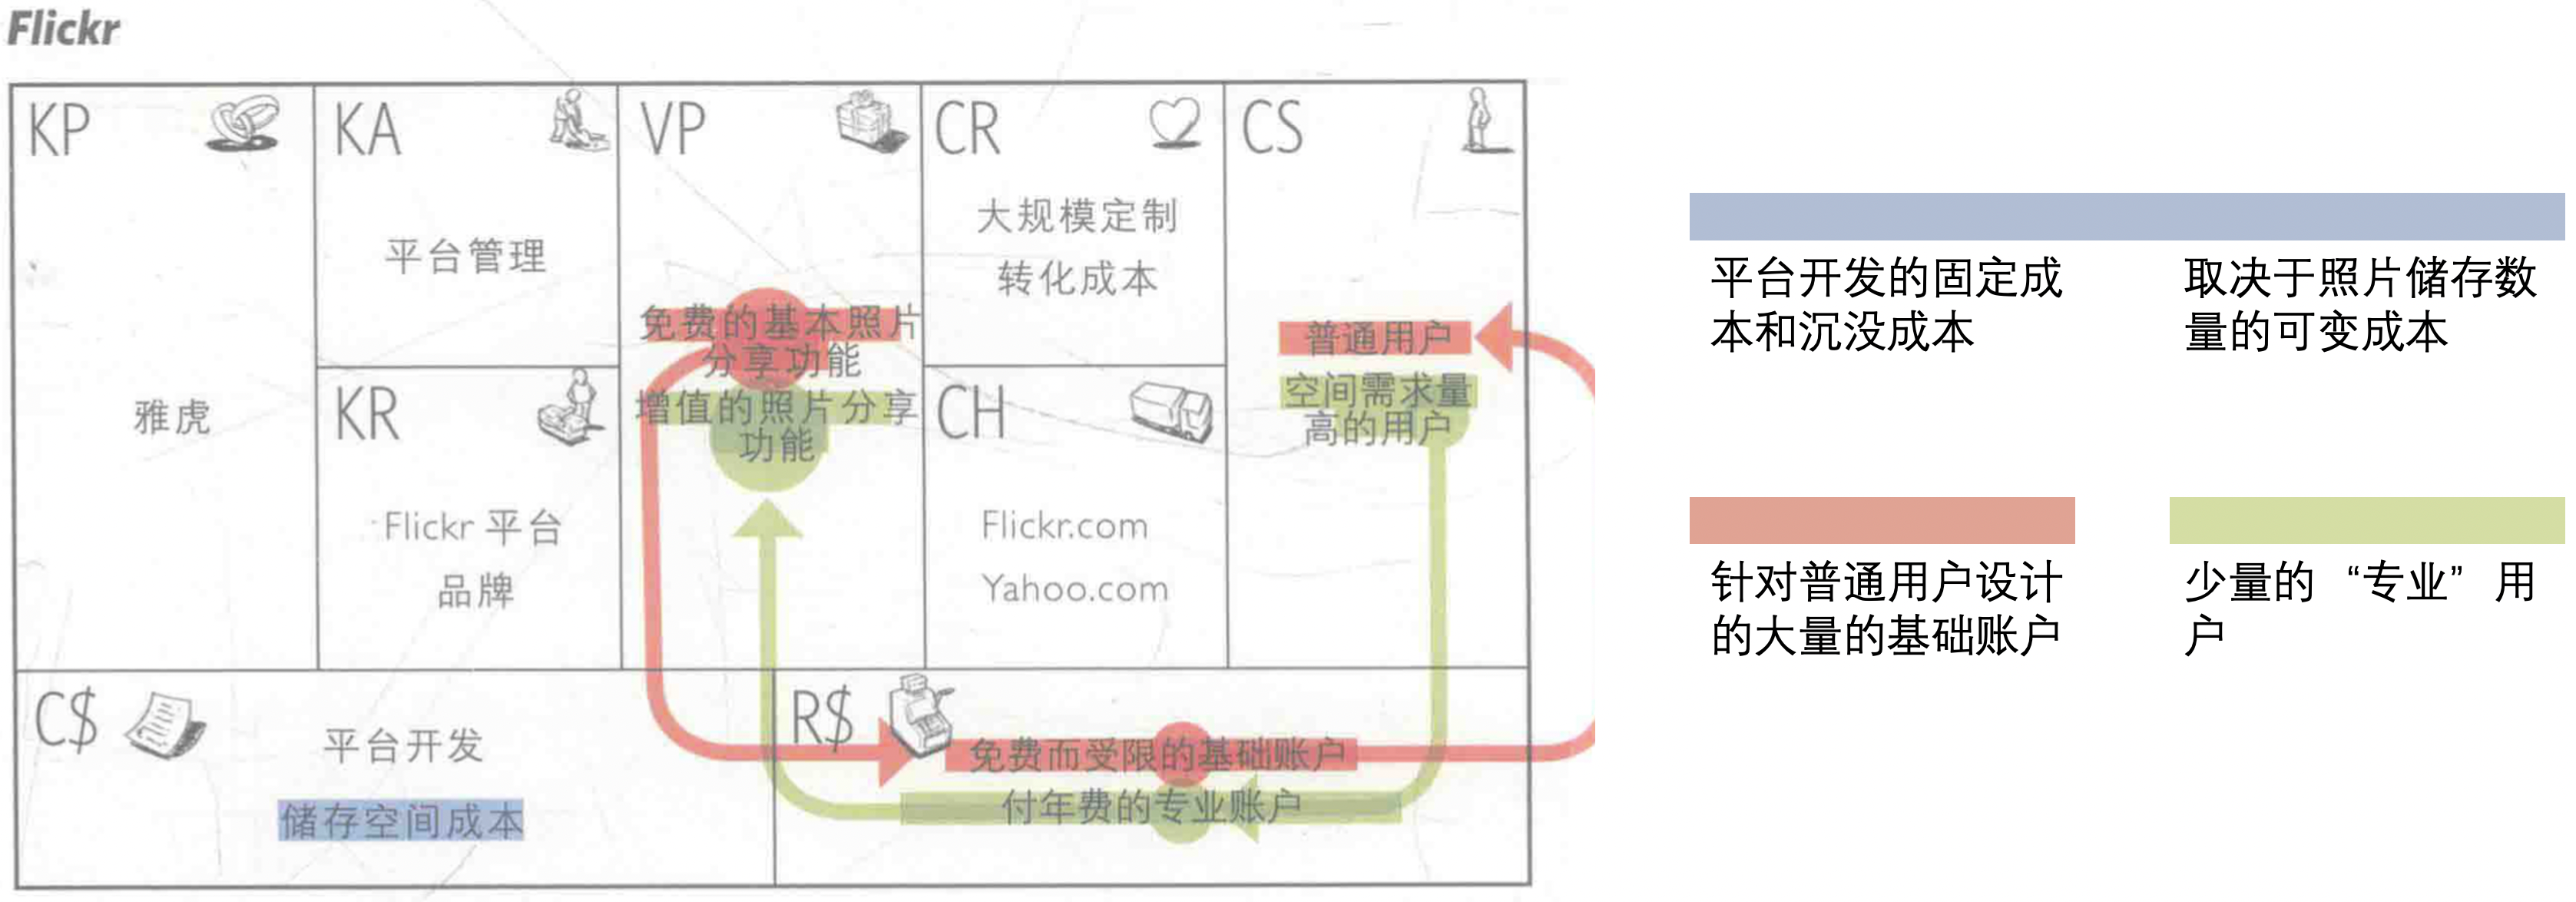
\includegraphics[width=0.98\textwidth]{img/Flicker的商业模式.png}
        \vspace{-0.5em}
	\end{figure}

    \paragraph{开放源码:与众不同的免费增值}~{}

    红帽公司(RedHat)将产品建立在开放源码的方式上。红帽公司明白,企业对耐用又免使用许可费的开放软件源码感兴趣,但因为没有任何实体对这些源码负责并提供维护而不愿使用它们。红帽公司填补了这个缺口,它免费提供稳定的、通过测试的、完整可使用的开放软件源码。
    \begin{itemize}
        \item 代码免费完整开放(多种许可证)
        \item 年费换取最新源码使用权、无限制服务支持、产品法律上拥有者联系的保证    
    \end{itemize}
    \begin{figure}[H]
		\centering
        \vspace{-0.5em}
		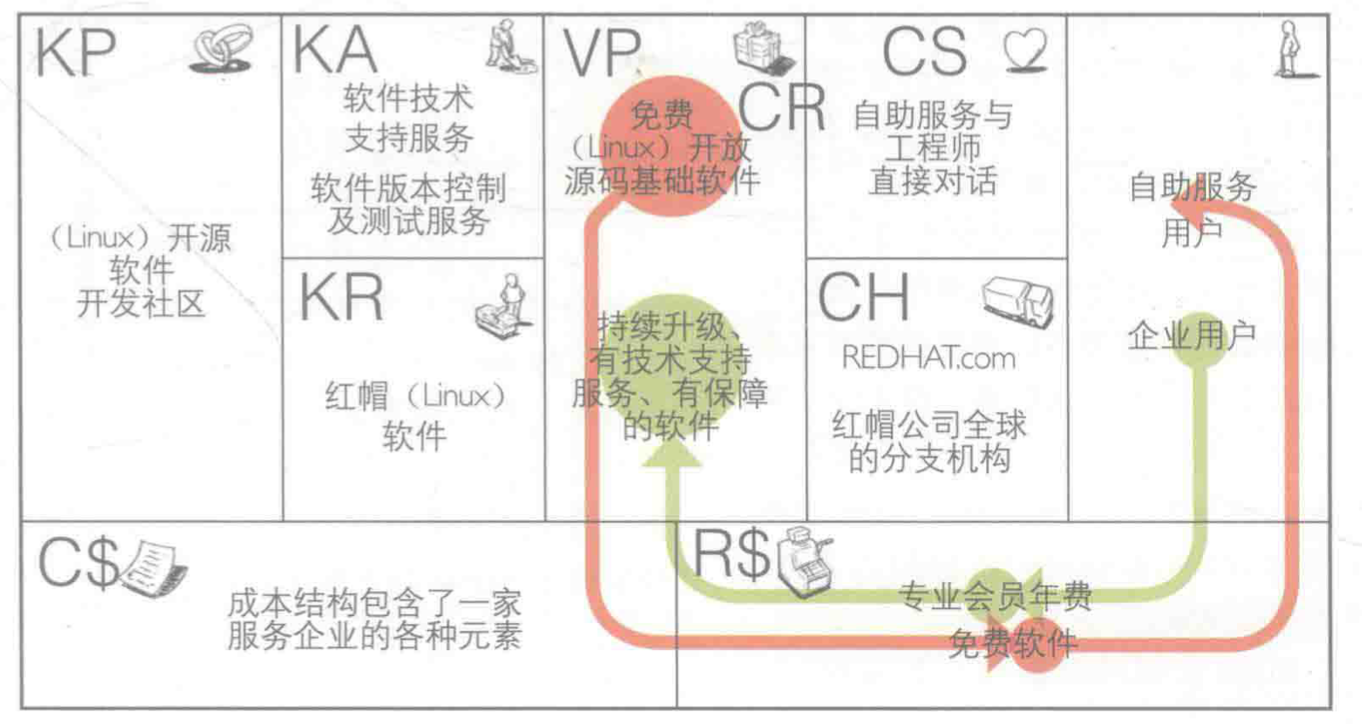
\includegraphics[width=0.7\textwidth]{img/RedHat的商业模式.png}
        \vspace{-0.5em}
	\end{figure}

    \paragraph{Skype的商业模式}~{}


    \begin{figure}[H]
		\centering
        \vspace{-0.5em}
		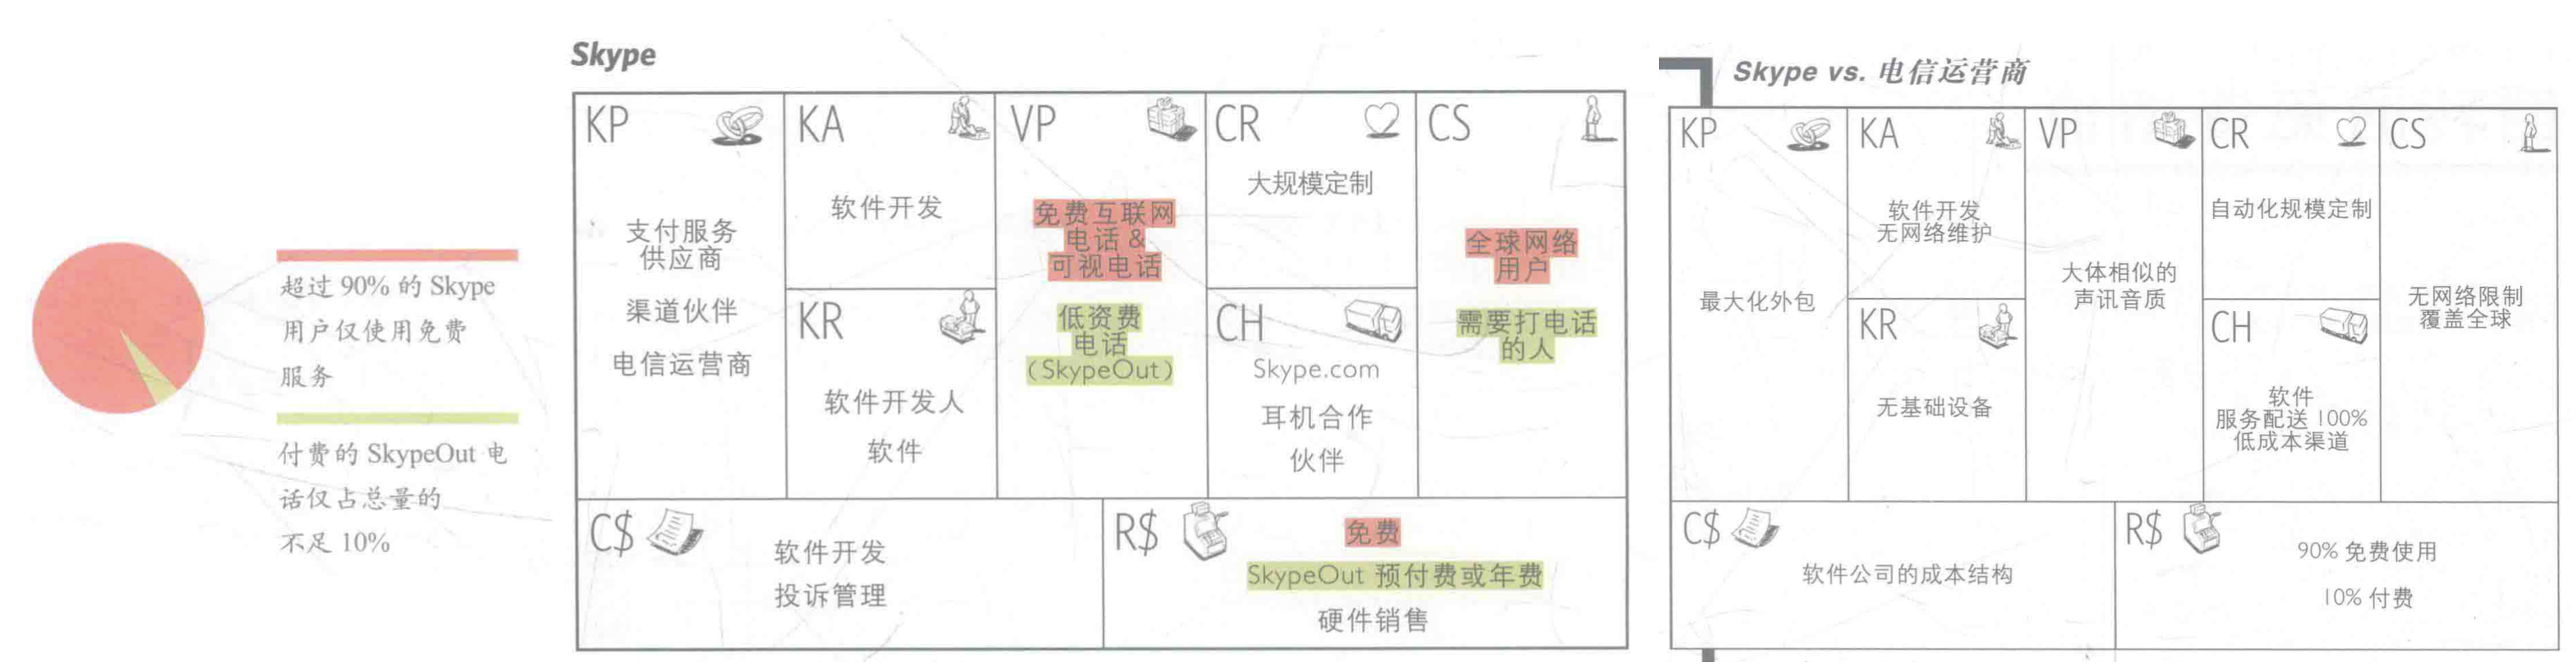
\includegraphics[width=\textwidth]{img/Skype的商业模式.png}
        \vspace{-0.5em}
	\end{figure}

    Skype以网络实现免费通话服务,对电信行业造成了破坏
    \begin{itemize}
        \item Skype公司开发了同名软件,可以安装于电脑或智能手机上,帮助用户之间实现设备间的免费通话
        \item Skype之所以能做到这一点是因为它的成本结构完全不同于电信运营商。免费电话的实现方式是路由互联网,基于对等计算技术,将用户的硬件设备和互联网当作通信的基础设备。因此,Skype不需要像电信运营商那样管理一套自有的网络设备,而只需要为每一位增加的用户支付少量的成本
        \item 用户只有在拨打固定电话的时候才需要付费,移动电话则通过一项叫作SkvpeOut的增值服务以非常低的费率享受与固定电话的通话服务
    \end{itemize}


    \paragraph{保险行业模式:倒转的免费增值}~{}

    在保险行业模式中,由大部分的客户定期支付小额保费以确保自己手虽不易发生却可能带来经济上的灾难的事件。简而言之,是大部分的付费客户来补贴那一小部分产生实际保险索赔的客户,但是任何一个付费客户都有可能随时变成受益群体中的一员。

    REGA是瑞士的一家非营利机构,它使用直升机和飞机将医护人员送到事故发生地点,这在多山的瑞士作用尤其显著。该组织有超过200万名“捐赠者”资助。作为回报,捐赠人免费享受REGA的一切救助。山间救援操作大多十分昂贵,因此REGA的捐赠者认为这样的服务十分有吸引力,可以帮助他们规避在滑雪假期、夏日徒步或者山间驾驶过程中,因可能发生的意外而支付高昂的救援花费。
    \begin{figure}[H]
		\centering
        \vspace{-0.5em}
		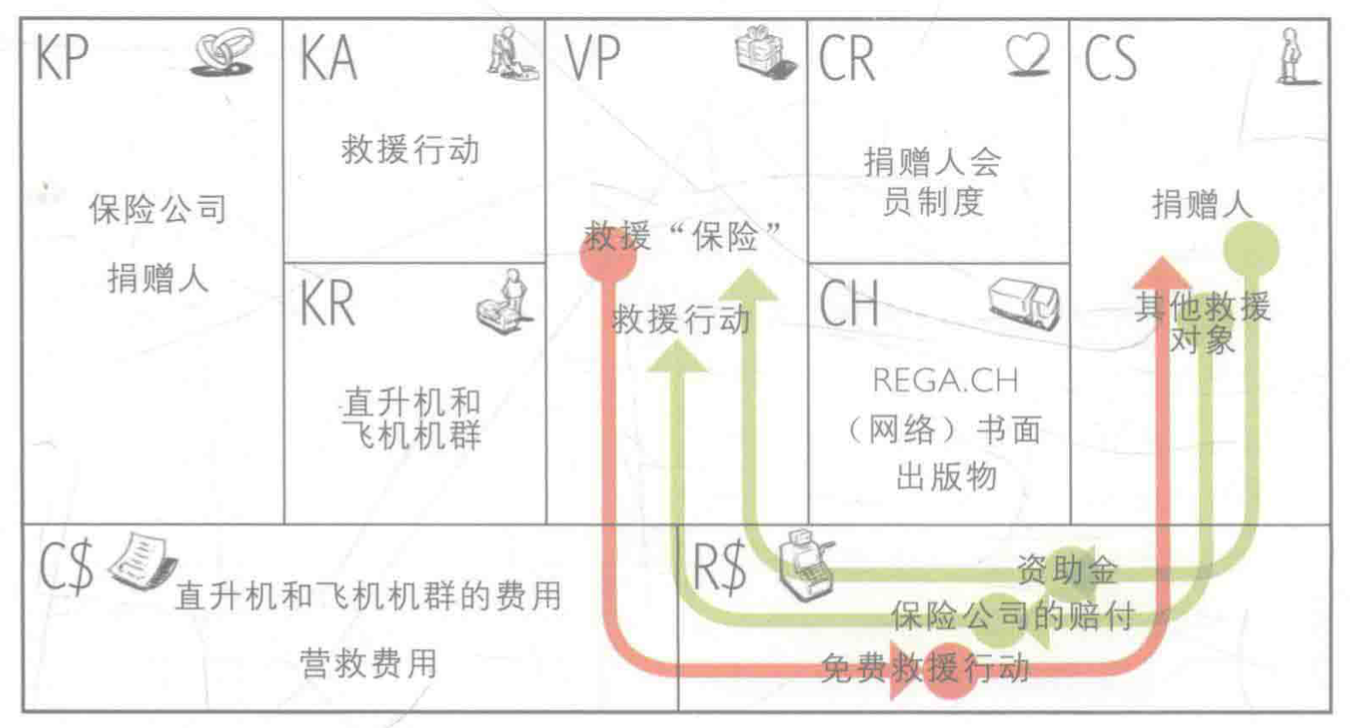
\includegraphics[width=0.7\textwidth]{img/保险行业模式.png}
        \vspace{-0.5em}
	\end{figure}

    \paragraph{免费增值模式总结}~{}

    \begin{itemize}
        \item 平台是免费增值模式最重要的资产,因为它使得免费的基础服务以低边际成本实现
        \item 客户关系是自动的且低成本的,因为有大量的免费用户数量
        \item 免费用户向增值用户的转化率,是一个很重要的衡量指标
        \item 该模式的成本结构分为三部分:可观的固定成本,为免费账户提供的低边际成本服务,以及(独立的)增值账户成本
        \begin{itemize}
            \item 收入 $=$ 用户数量 $\times$ 增值用户比重 $\times$ 增值服务价格 $\times$ 增长率 $\times$ 顾客流失
            \item 服务成本 $=$ 免费用户数 $\times$ 免费服务成本 $+$ 增值用户数 $\times$ 增值服务成
            \item 运营利润 $=$ 收入 $-$ 服务成本 $-$ 固定成本 $-$ 获客成本
        \end{itemize}
    \end{itemize}

    \begin{figure}[H]
		\centering
        \vspace{-0.5em}
		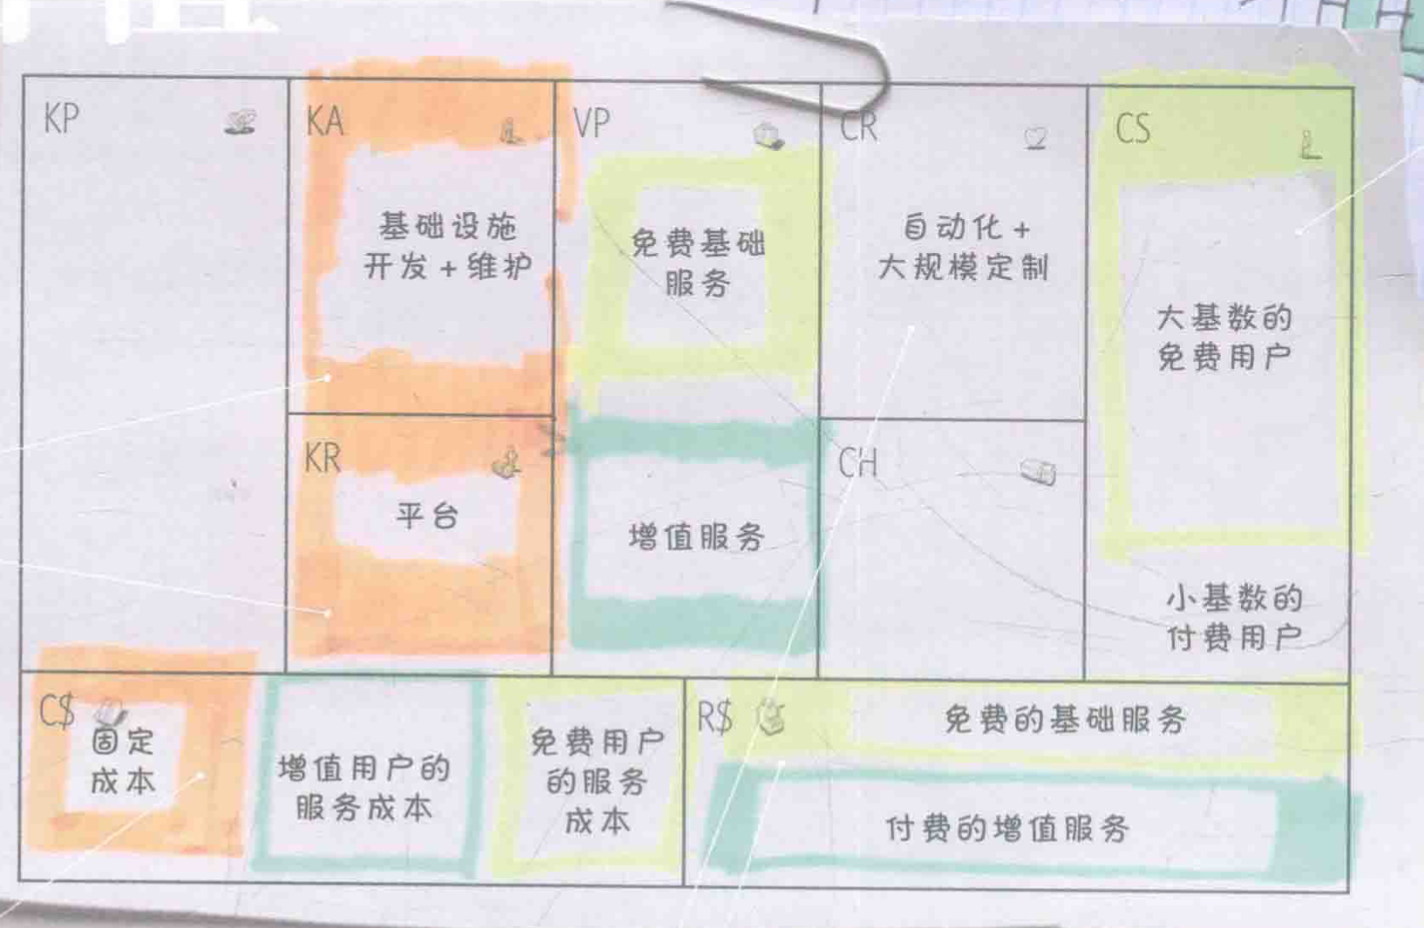
\includegraphics[width=0.7\textwidth]{img/免费增值模式总结.png}
        \vspace{-0.5em}
	\end{figure}

    \subsubsection{诱饵\&陷阱模式}

    诱饵\&陷阱模式的特点是期初以不贵的或者免费的价格提供有吸引力的商品,且该商品还将进一步地鼓励对相关产品或服务的不断消费
    \begin{itemize}
        \item 这一模式也被称作“招徕定价”或者“剃刀\&刀片”模式
        \begin{itemize}
            \item “招徕定价”是指期初以补贴价格,甚至亏本的价格提供商品,意图通过后续消费获得利润
            \item “剃刀\&刀片”模式是指因发明了一次性刀片而风靡的商业模式
        \end{itemize}
        \item 举例:剃刀+一次性刀片,打印机+墨盒/硒鼓,合约机等
    \end{itemize}

    \begin{figure}[H]
		\centering
        \vspace{-0.5em}
		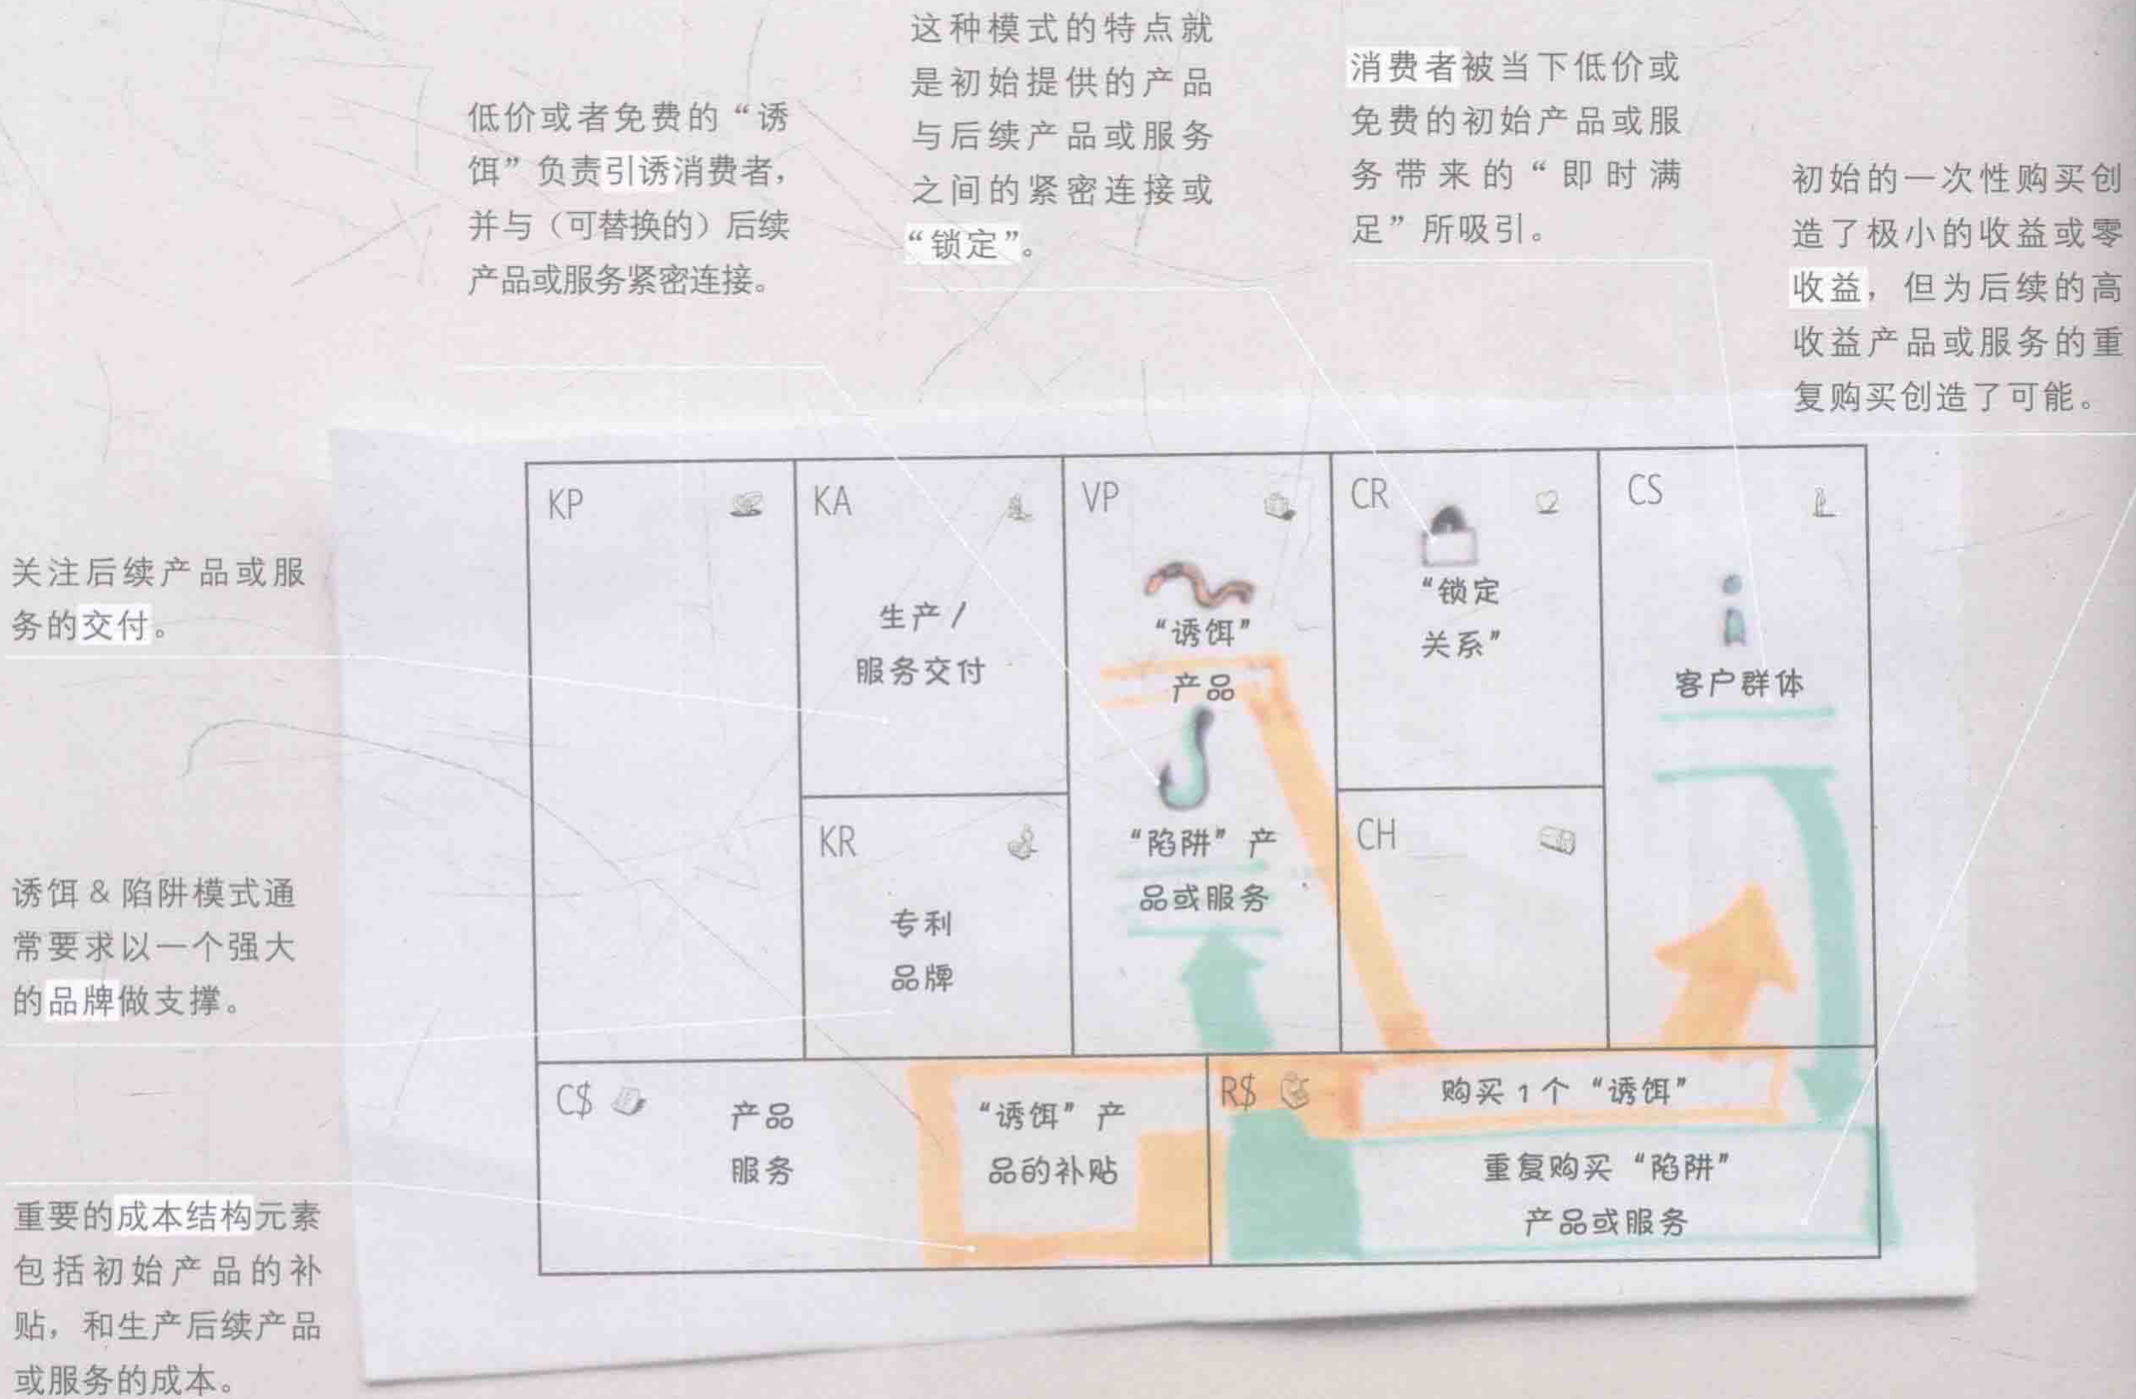
\includegraphics[width=0.8\textwidth]{img/诱饵&陷阱模式.png}
        \vspace{-0.5em}
	\end{figure}

    \subsection{开放式商业模式}
    开放的商业模式适用于通过与外部合作伙伴系统地配合而创造和获取价值的企业。这种模式可以是“由外而内”地于企业内部尝试来自外部的理念,或者“由内而外”地向外部合作伙伴输出公司无用的理念或资产。

    \begin{figure}[H]
		\centering
        \vspace{-0.5em}
		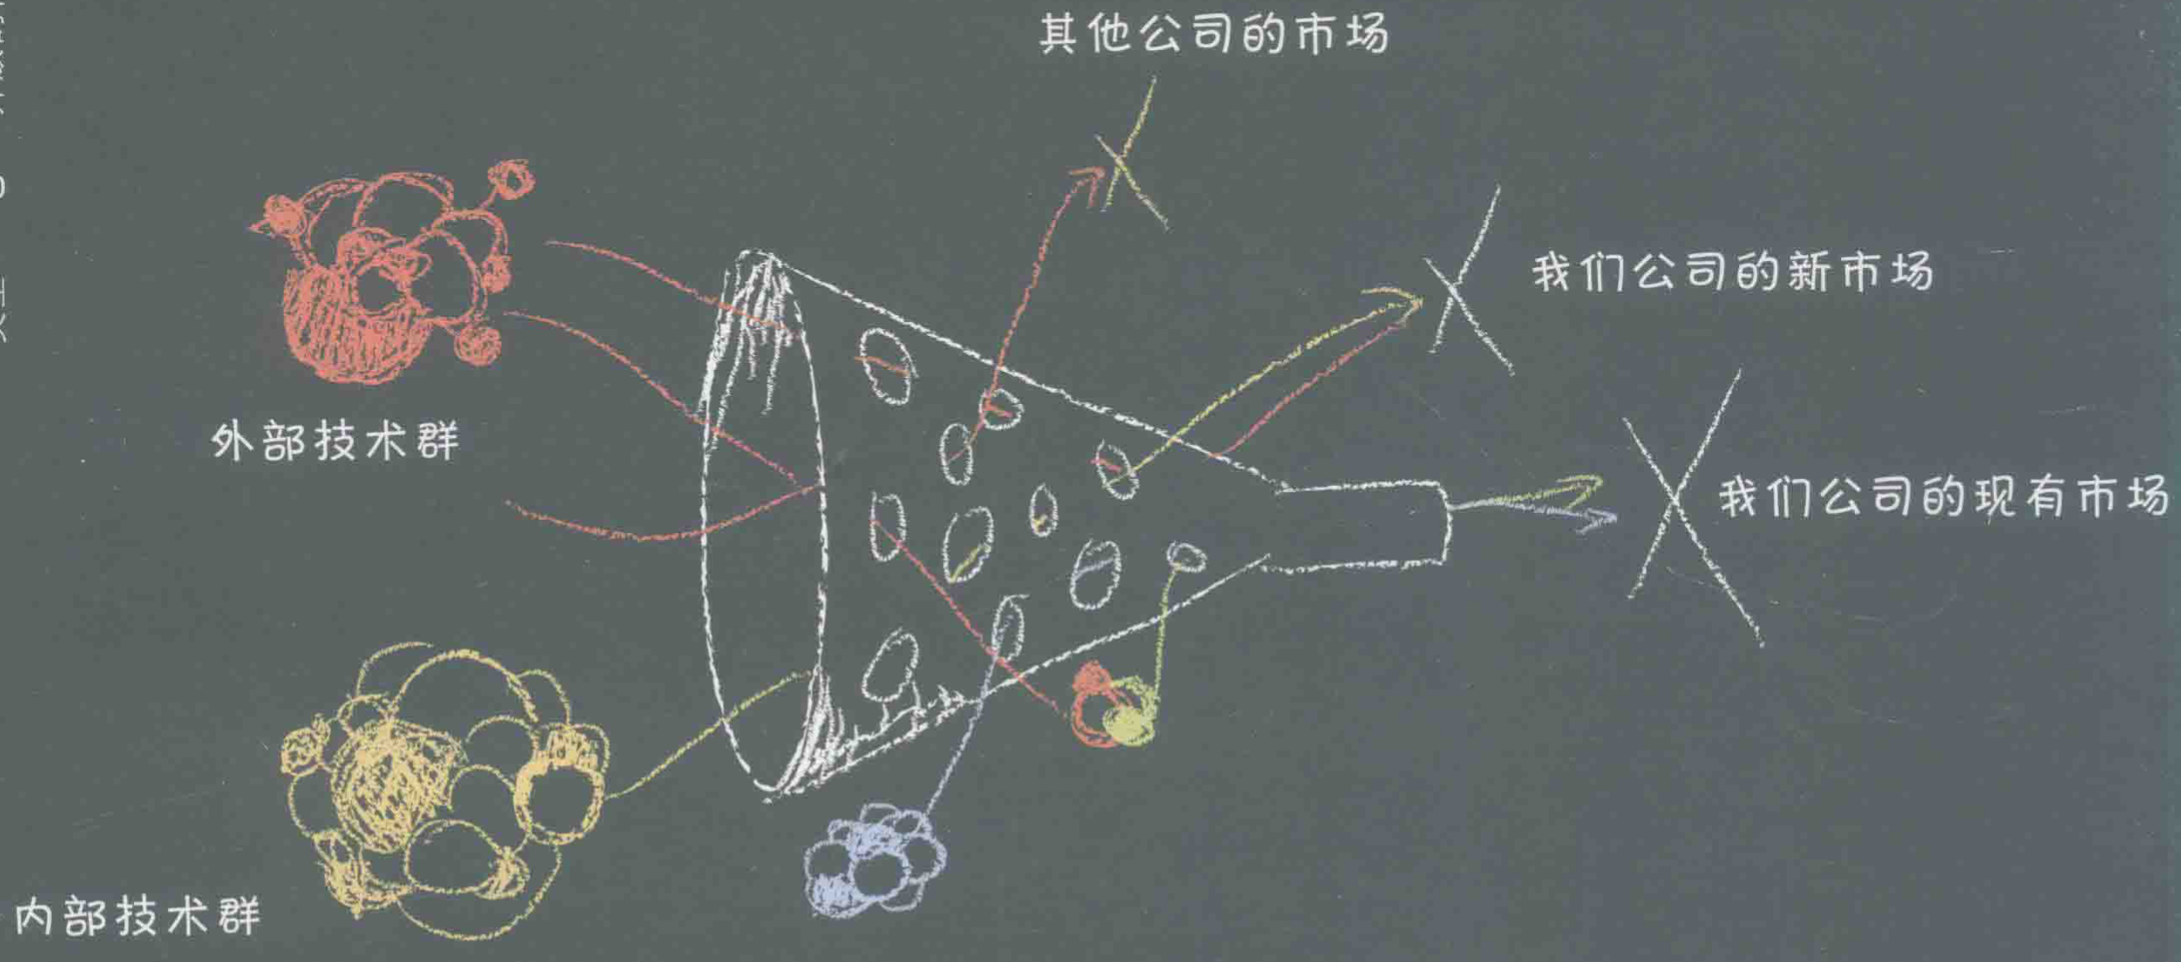
\includegraphics[width=0.55\textwidth]{img/开放的商业模式.png}
        \vspace{-0.5em}
	\end{figure}

    “开放式的创新”和“开放的商业模式”是由亨利·切萨布鲁夫提出的两个术语。它们意指将企业的研发流程向外界敞开
    \begin{itemize}
        \item 切萨布鲁夫主张,在一个以发散的知识为特征的世界中,组织可以通过将外部的知识、知识产权和产品整合进自身的创新流程,进而创造更大的价值并更好地利用自己的研发能力
        \item 此外,切萨布鲁夫演示了,对某家企业而言无用的产品、技术、知识和知识产权可以通过同意许可、合资或者剥离的方式供给外部团体使用,从而变现
        \item 切萨布鲁夫将“由外而内”的创新和“由内而外”的创新区分开来
        \begin{itemize}
            \item “由外而内”的创新发生于当组织将来自外部的理念技术或知识产权引入自身的发展和商业流程
            \item “由内而外”的创新发生于当组织同意许可或出售其知识产权或技术,尤其是闲置资产
        \end{itemize}
    \end{itemize}

    \begin{figure}[H]
		\centering
        \vspace{-0.5em}
		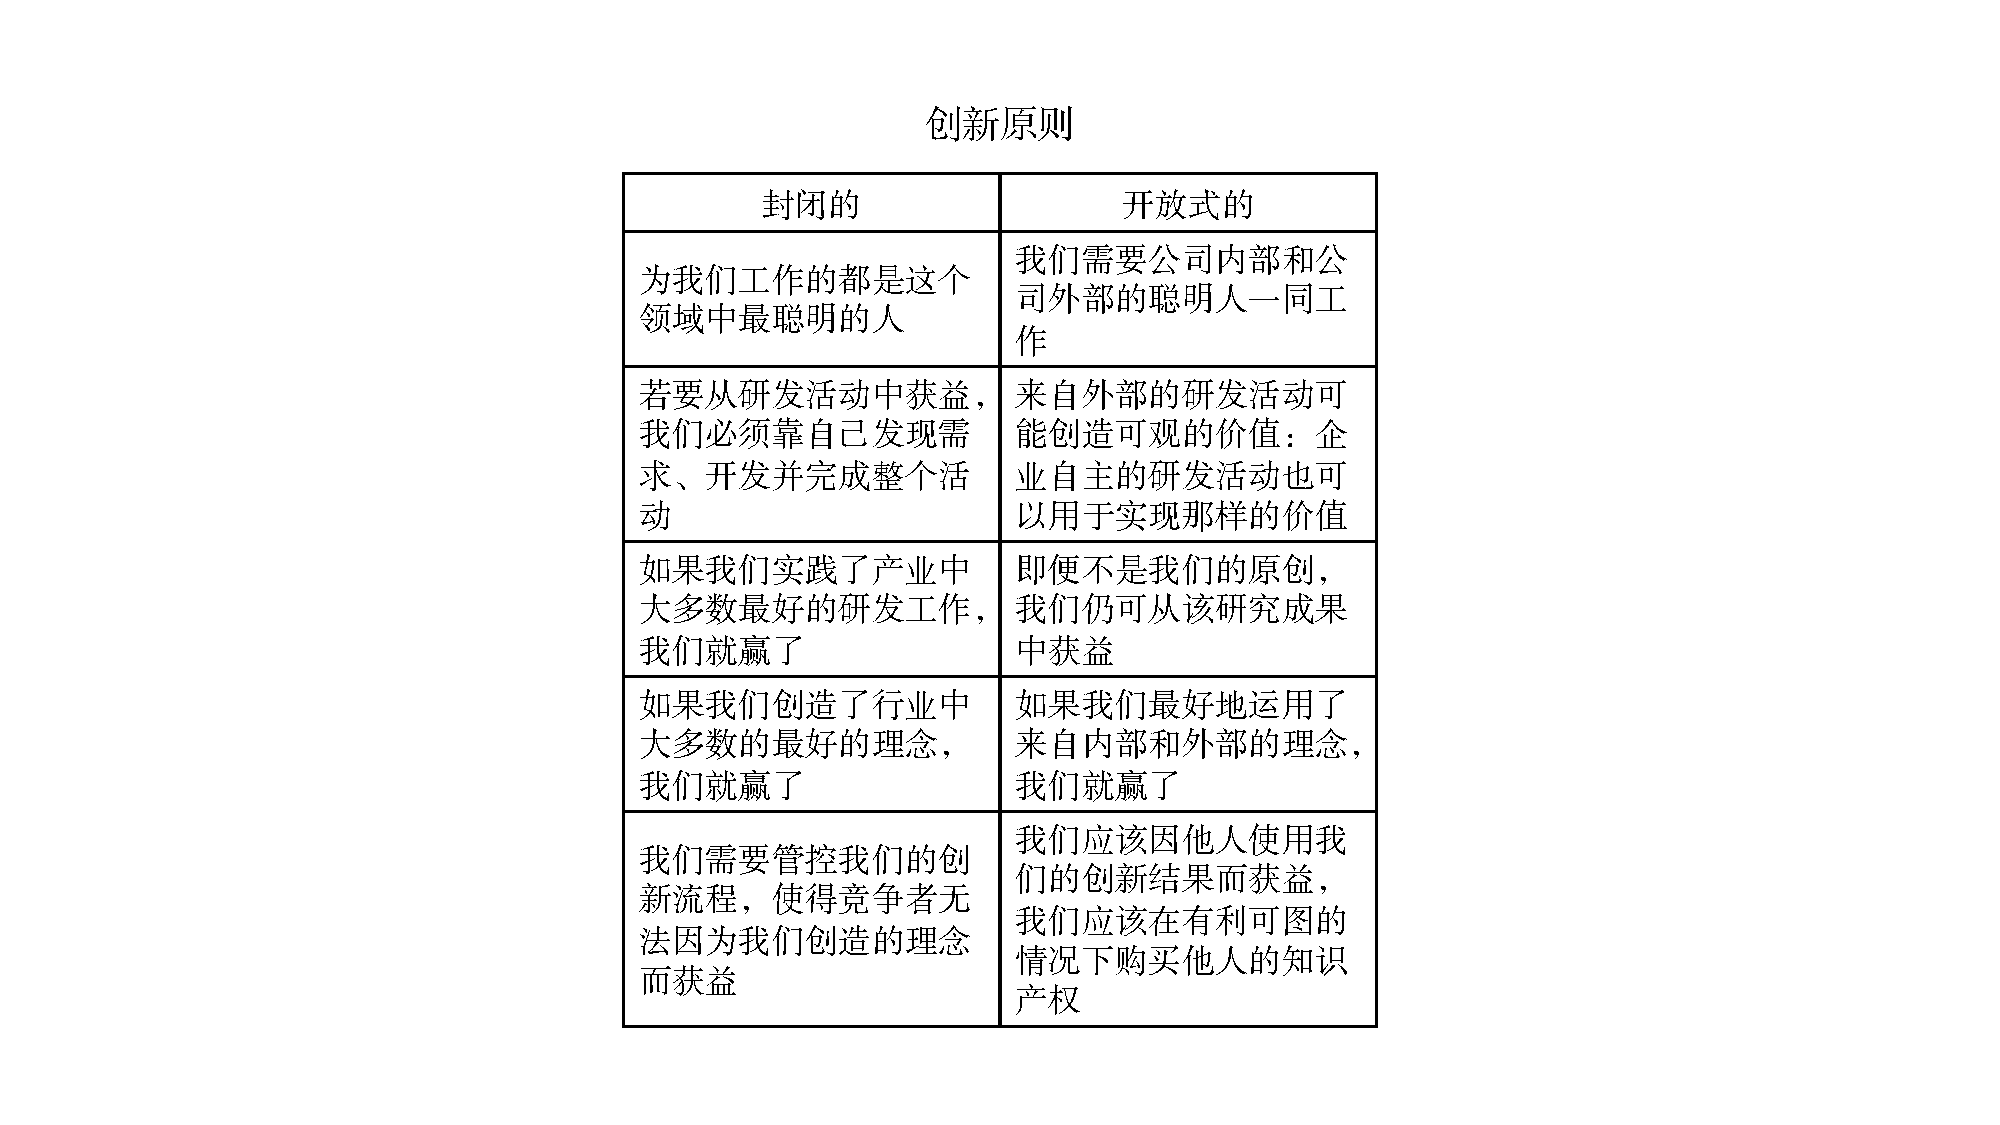
\includegraphics[width=0.4\textwidth]{img/创新原则.pdf}
        \vspace{-0.5em}
	\end{figure}

    \subsubsection{宝洁:连接\&发展}
    宝洁挽救公司的举措是建立一套新的创新开放体系:聚焦于内部研发的方式转变为开放式的研发流程,关键因素就是实施“连接\&发展”战略,旨在通过外部合作方力量拉动内部的研发活动
    \begin{figure}[H]
		\centering
        \vspace{-0.5em}
		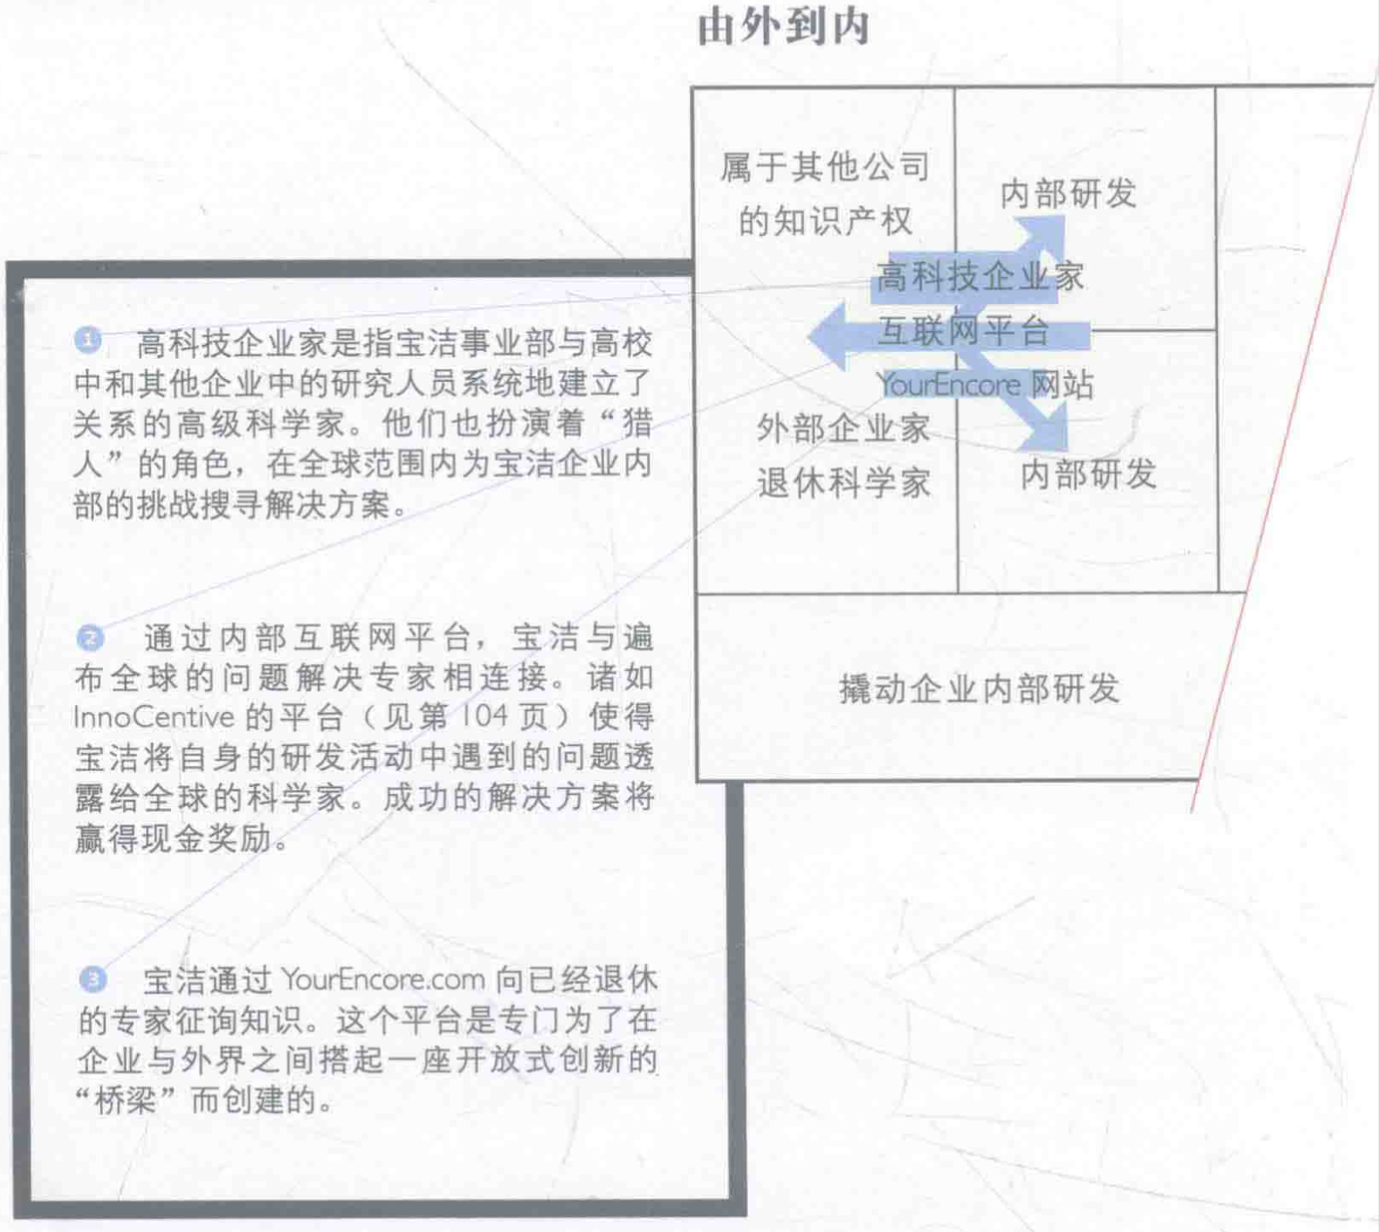
\includegraphics[width=0.6\textwidth]{img/宝洁.png}
        \vspace{-0.5em}
	\end{figure}

    \subsubsection{葛兰素史克的专利池}
    由外而内的开放式创新方法是将企业内部的闲置资产变现,主要针对专利和技术
    \begin{itemize}
        \item 葛兰素史克的目标是提高世界上最贫困国家的药物普及率,以及在研究不足的疾病领域投入更多的研发
        \item 葛兰素史克建立的专利池,主要放置和治疗疾病相关的知识产权,并对外开放,避免研发进度由个别专利人阻挠而停滞
        \begin{itemize}
            \item 停止在50个最不发达地区申请或主张专利(允许仿制)
        \end{itemize}
    \end{itemize}
    
    \begin{figure}[H]
		\centering
        \vspace{-0.5em}
		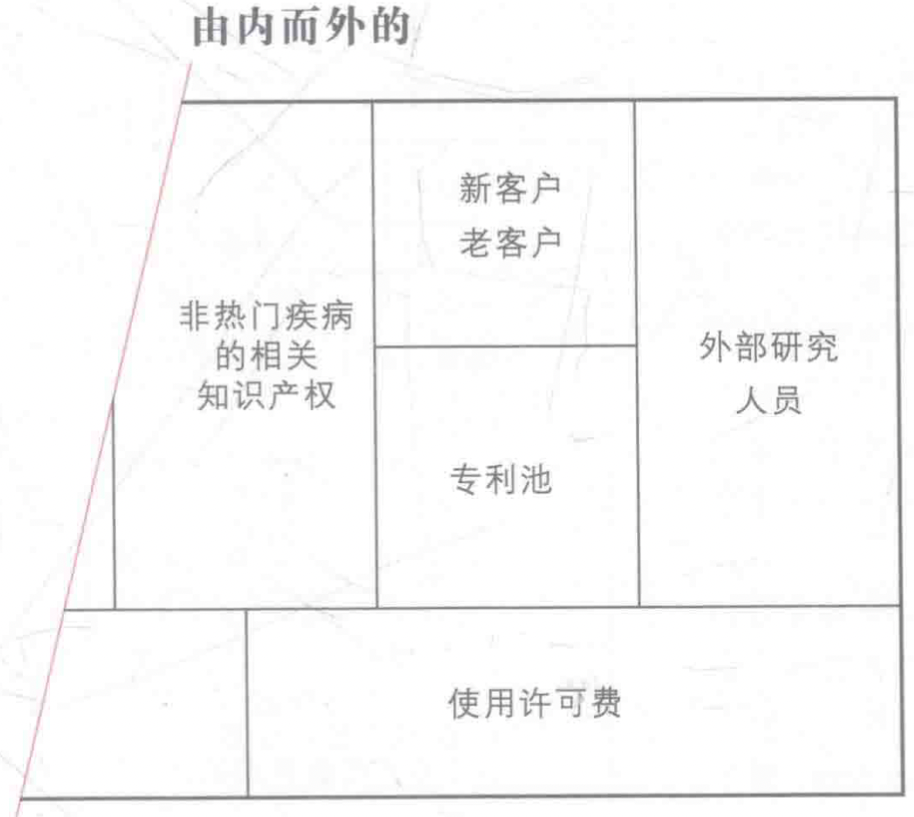
\includegraphics[width=0.4\textwidth]{img/葛兰素史克.png}
        \vspace{-0.5em}
	\end{figure}

    \subsubsection{连接器:InnoCentive}
    企业向外部的研究人员寻求灵感也有可能产生可观的成本,例如当企业有目的地吸引某些人才或企业的合作,而这些人才或企业拥有能够为其解决自身问题提供帮助的知识时。另外,当某企业的研究人员试图在该企业以外使用自己的知识时,为了找到有吸引力的机会,同样会发生搜索成本。
    \begin{itemize}
        \item InnoCentive就是为有研发问题需要解决的组织和全世界范围内有强烈意愿去解决具有挑战性的问题的研究人员提供一个连接,目前发展为一家独立的中介机构。
    \end{itemize}
    
    \begin{figure}[H]
		\centering
        \vspace{-0.5em}
		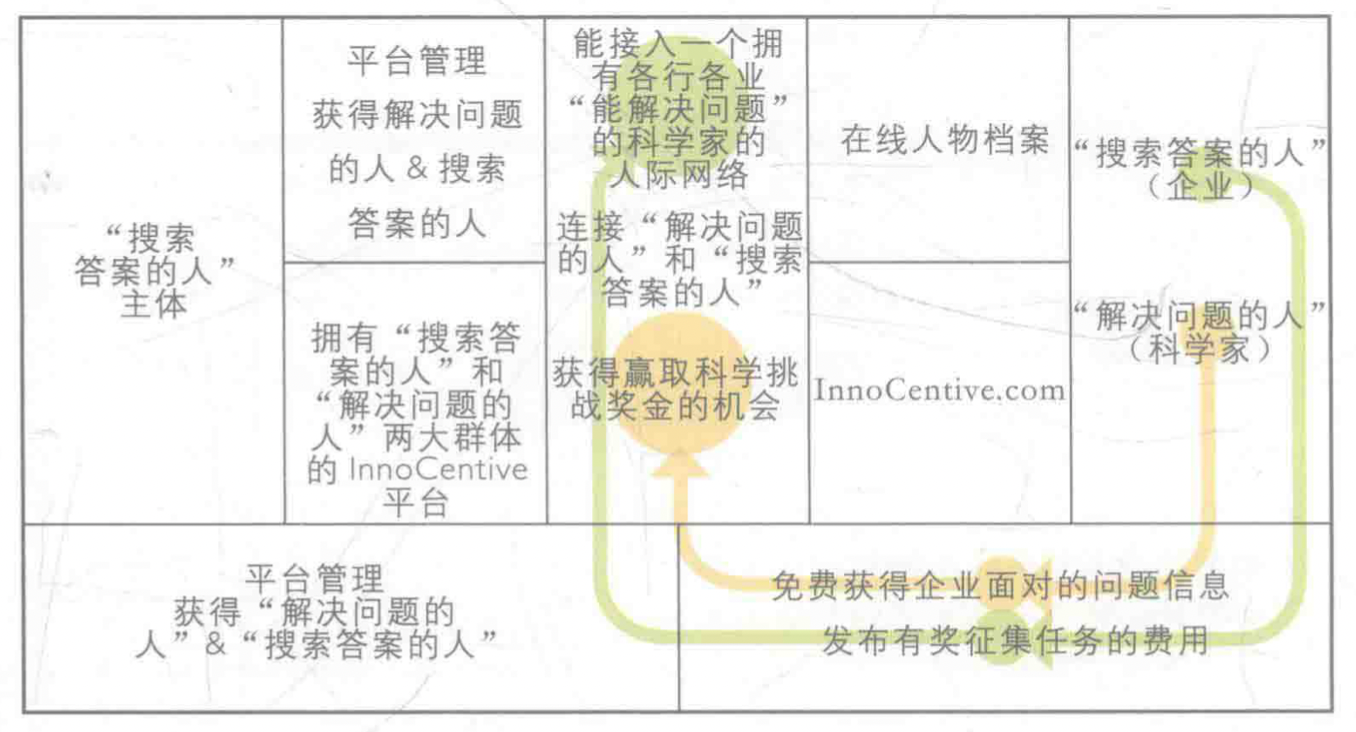
\includegraphics[width=0.6\textwidth]{img/InnoCentive.png}
        \vspace{-0.5em}
	\end{figure}

    \subsubsection{由外而内的模式总结}
    \begin{figure}[H]
		\centering
        \vspace{-0.5em}
		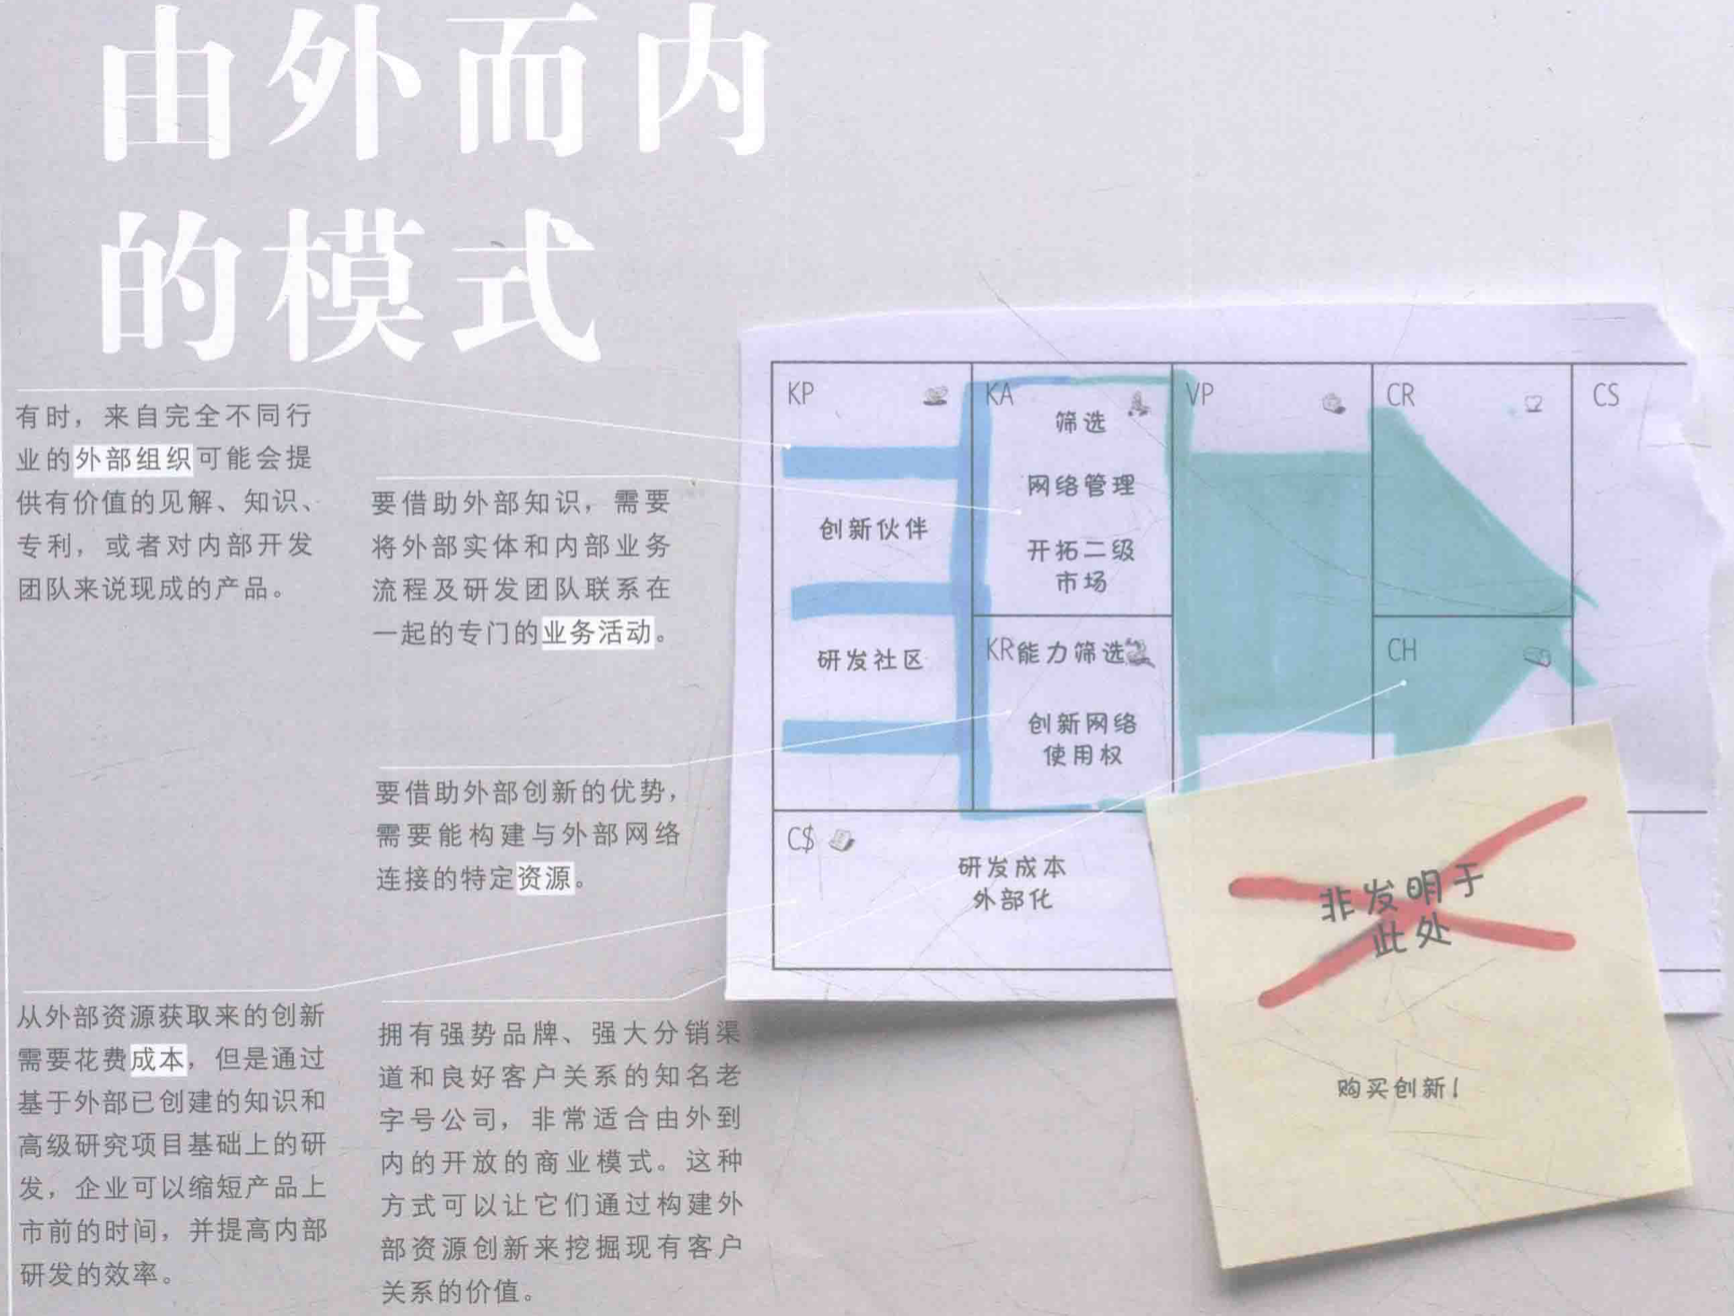
\includegraphics[width=0.7\textwidth]{img/由外而内的模式.png}
        \vspace{-0.5em}
	\end{figure}
    
    \subsubsection{由内到外的模式总结}
    \begin{figure}[H]
		\centering
        \vspace{-0.5em}
		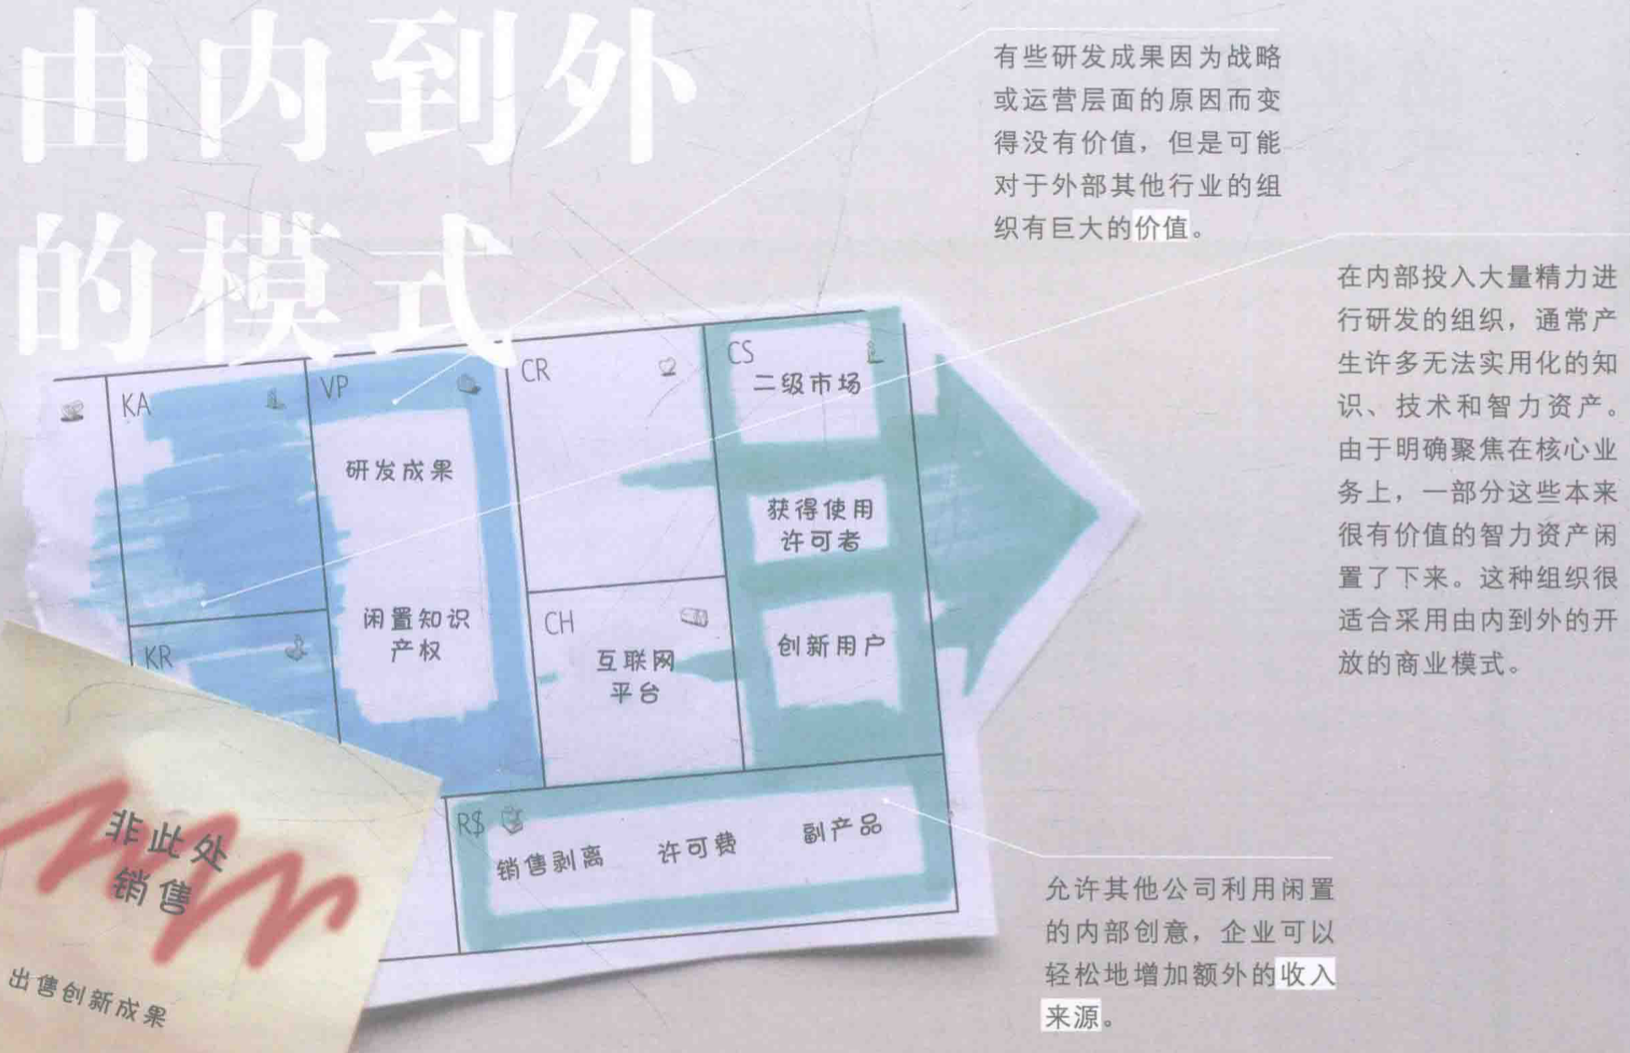
\includegraphics[width=0.7\textwidth]{img/由内到外的模式.png}
        \vspace{-0.5em}
	\end{figure}

    \subsection{商业模式类型总结}
    \begin{figure}[H]
		\centering
        \vspace{-0.5em}
		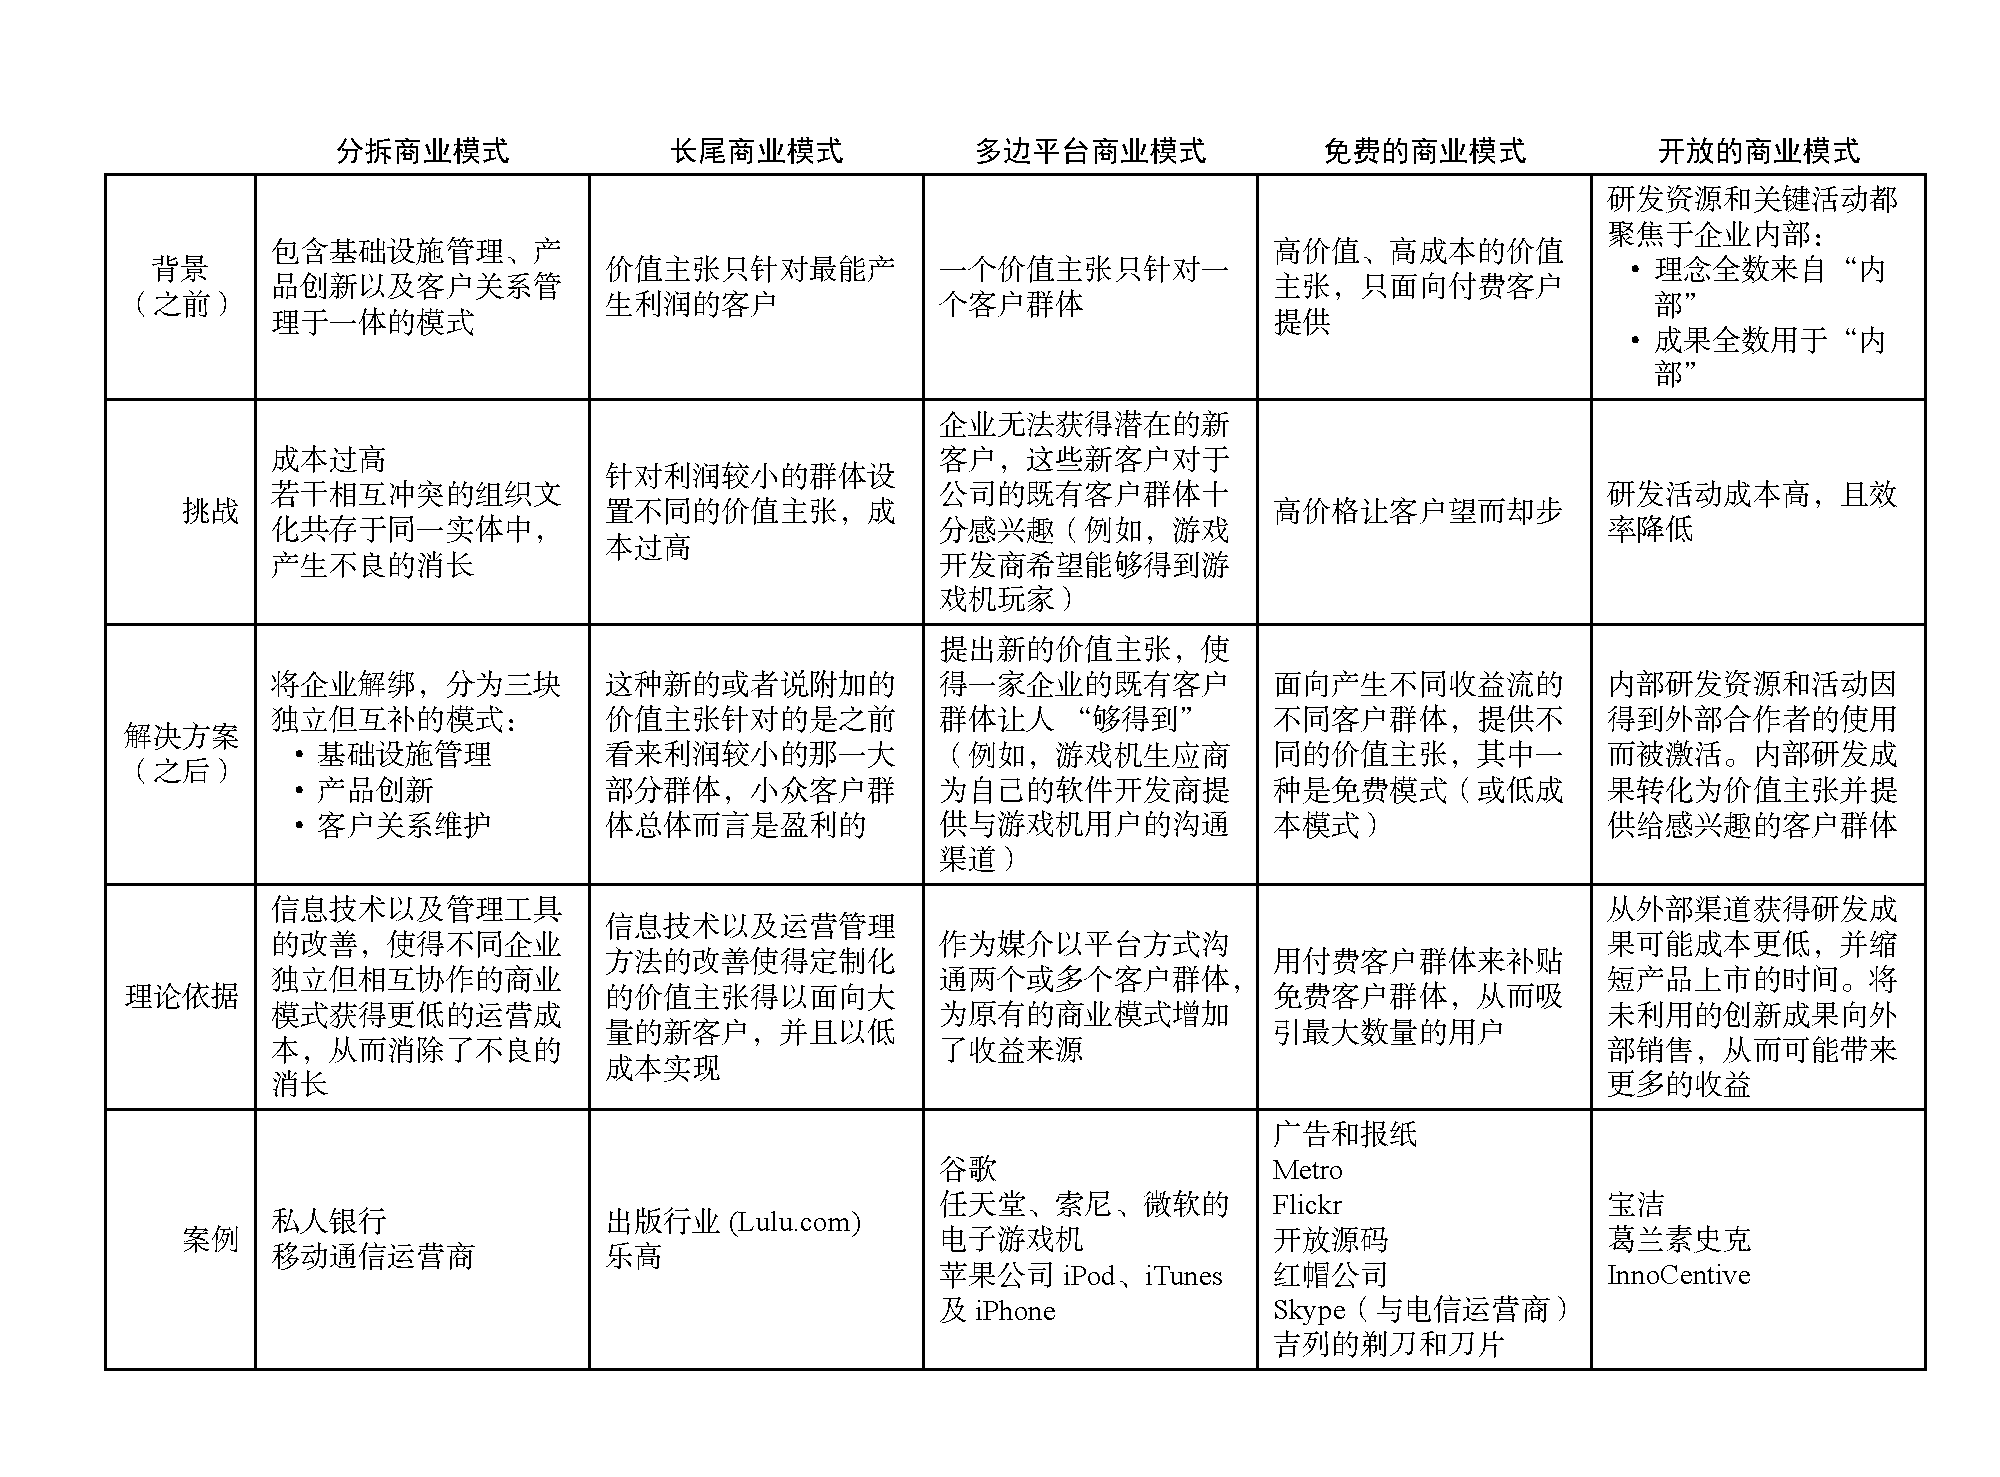
\includegraphics[width=\textwidth]{img/商业模式总结.pdf}
        \vspace{-0.5em}
	\end{figure}


















	\section{商业模式设计}

商业模式设计方法有:\textbf{客户洞察}、\textbf{构思}、\textbf{视觉化思考}、\textbf{模型构建}、\textbf{讲故事}和\textbf{场景}。

\subsection{客户洞察}

客户视角是商业模式设计的指导性原则。客户的观点决定了我们选择怎样的价值主张、渠道、客户关系和收益来源。

企业一般都会在市场研究上投入重金,但它们最终设计产品、服务和商业模式的时候往往又会忽略客户的观点。要想设计好的商业模式,必须避免这类错误
\begin{itemize}
    \item 必须通过客户的眼睛来观察商业模式,这样就有可能发现全新的机会。
    \item 难点在于对客户透彻的理解。商业模式的设计必须基于这份理解。在产品和服务设计领域,很多业界领先的企业都通过与社会学家一起合作来加深他们的理解。
    \item 创新的真正挑战在于深入理解客户,而不是简单地去问他们要什么。
    \begin{itemize}
        \item  汽车工业的先驱亨利·福特曾经说过:“要是我去问客户他们想要什么,他们会要一匹更快的马。”
    \end{itemize}
    \item 另一个难点在于企业是否清楚需要关注哪些客户、忽略哪些客户。
    \begin{itemize}
        \item 在很多情况下,能够拉动未来增长的那些客户往往并不是今天的金牛客户。
        \item 商业模式的创新不能仅仅聚焦现有的客户群体,必须着眼于新客户群体。
    \end{itemize}
\end{itemize}

\subsubsection{移情图}
\begin{figure}[H]
	\centering
	\vspace{-0.5em}
	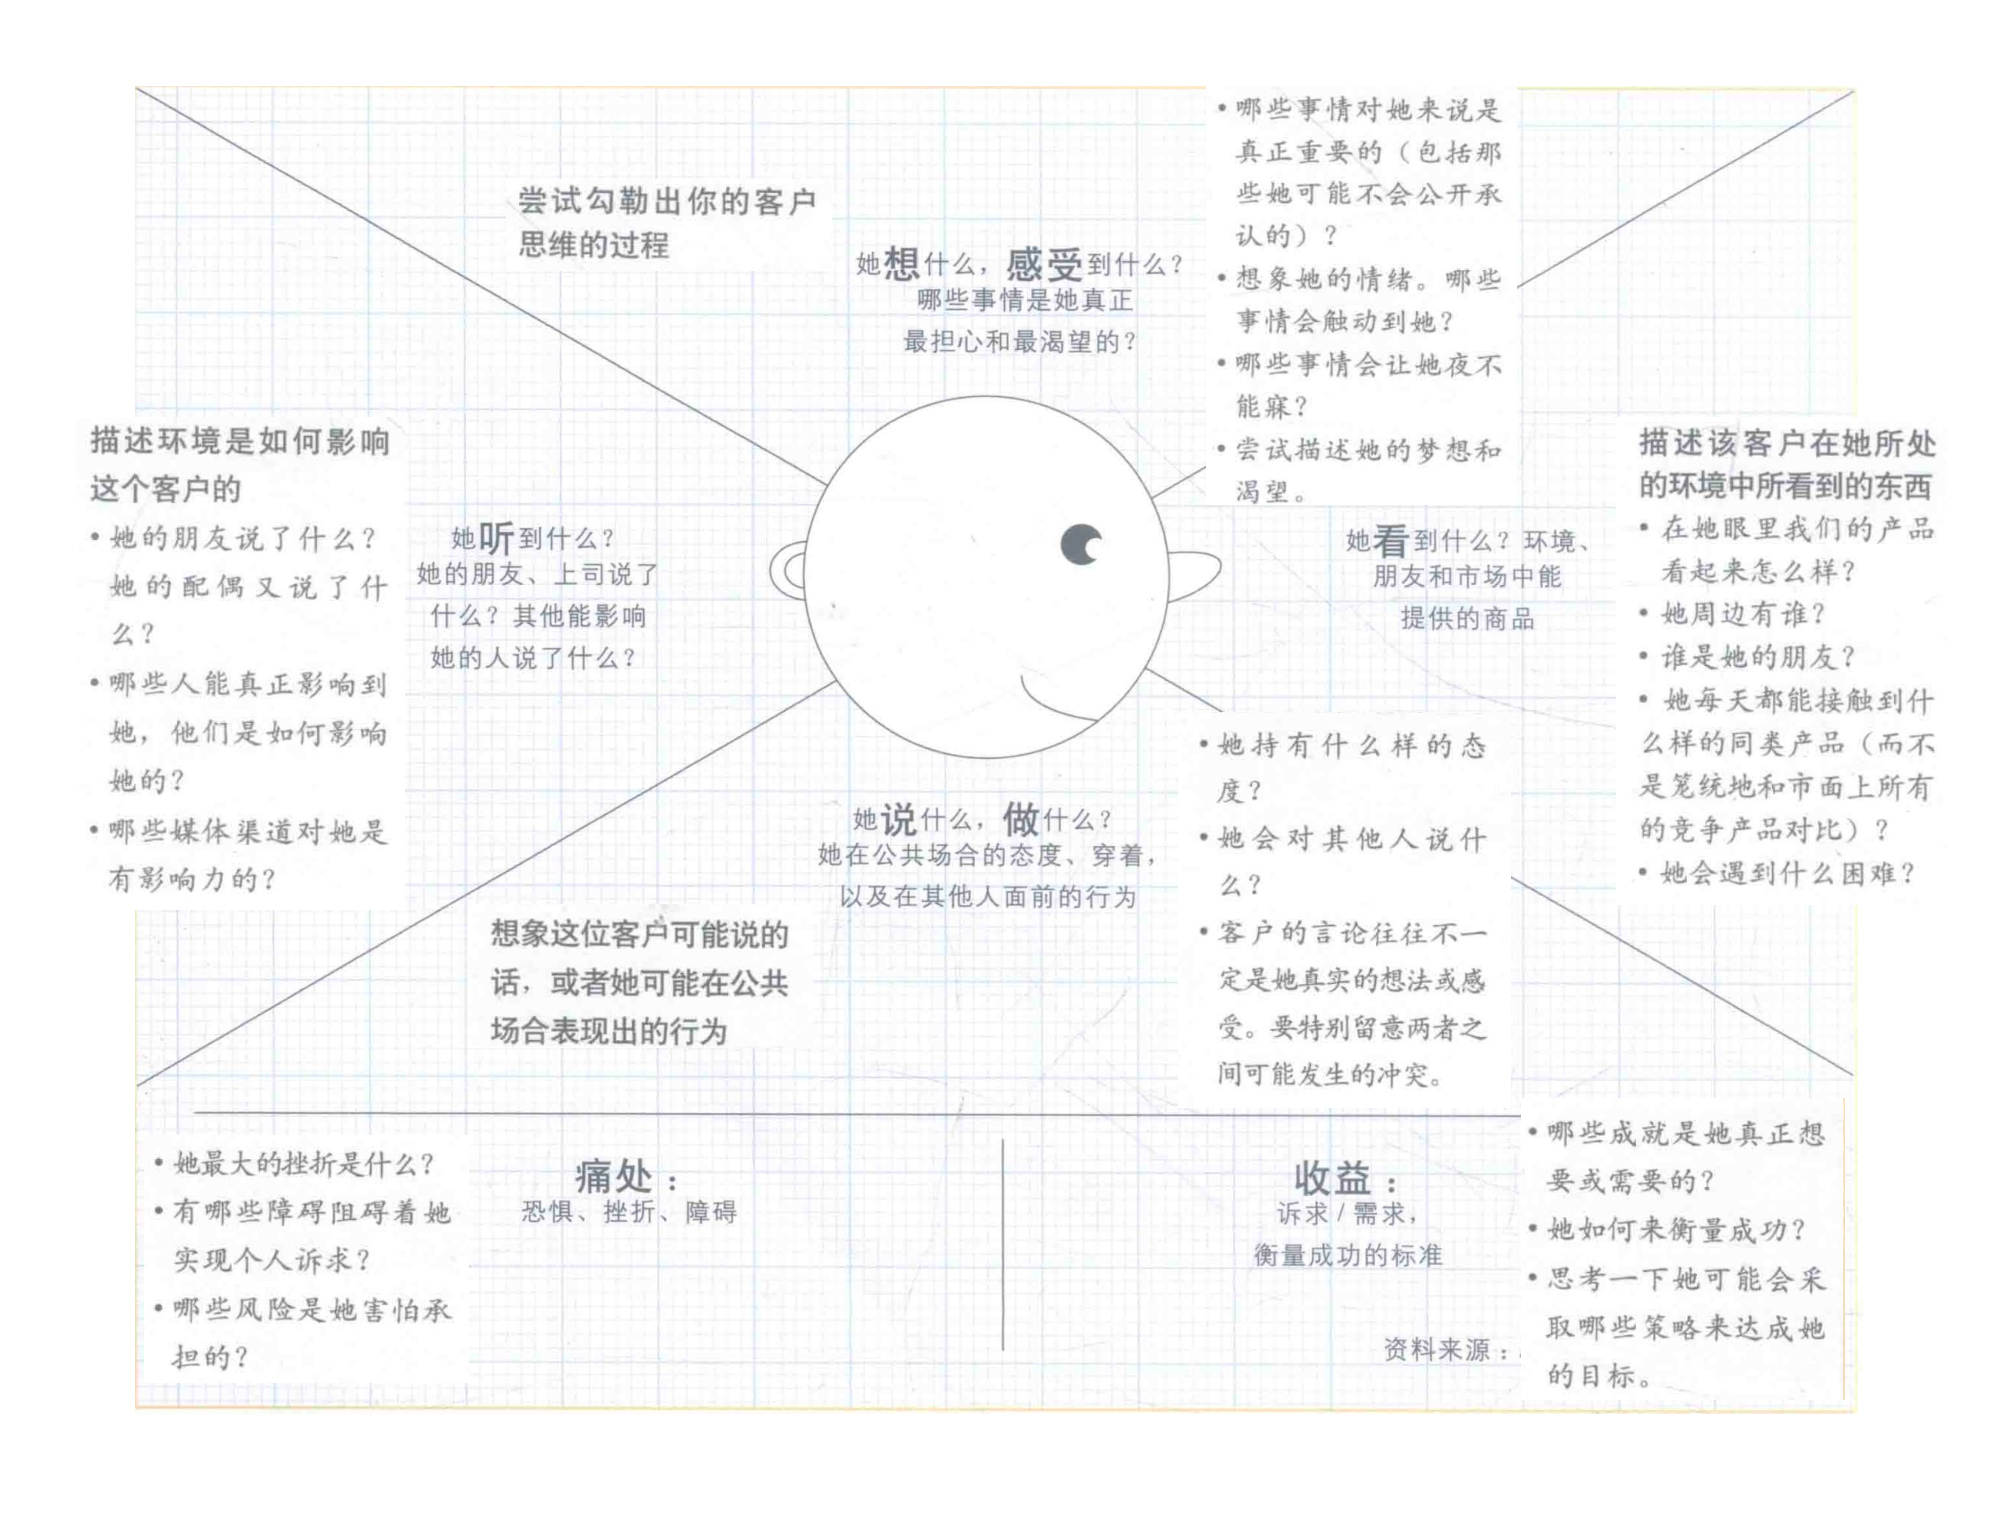
\includegraphics[width=0.95\textwidth]{img/移情图.pdf}
    \vspace{-1em}
\end{figure}

移情图示例:微软在线Office产品对于目标企业的首席信息官CIO

\begin{figure}[H]
	\centering
	\vspace{-0.5em}
	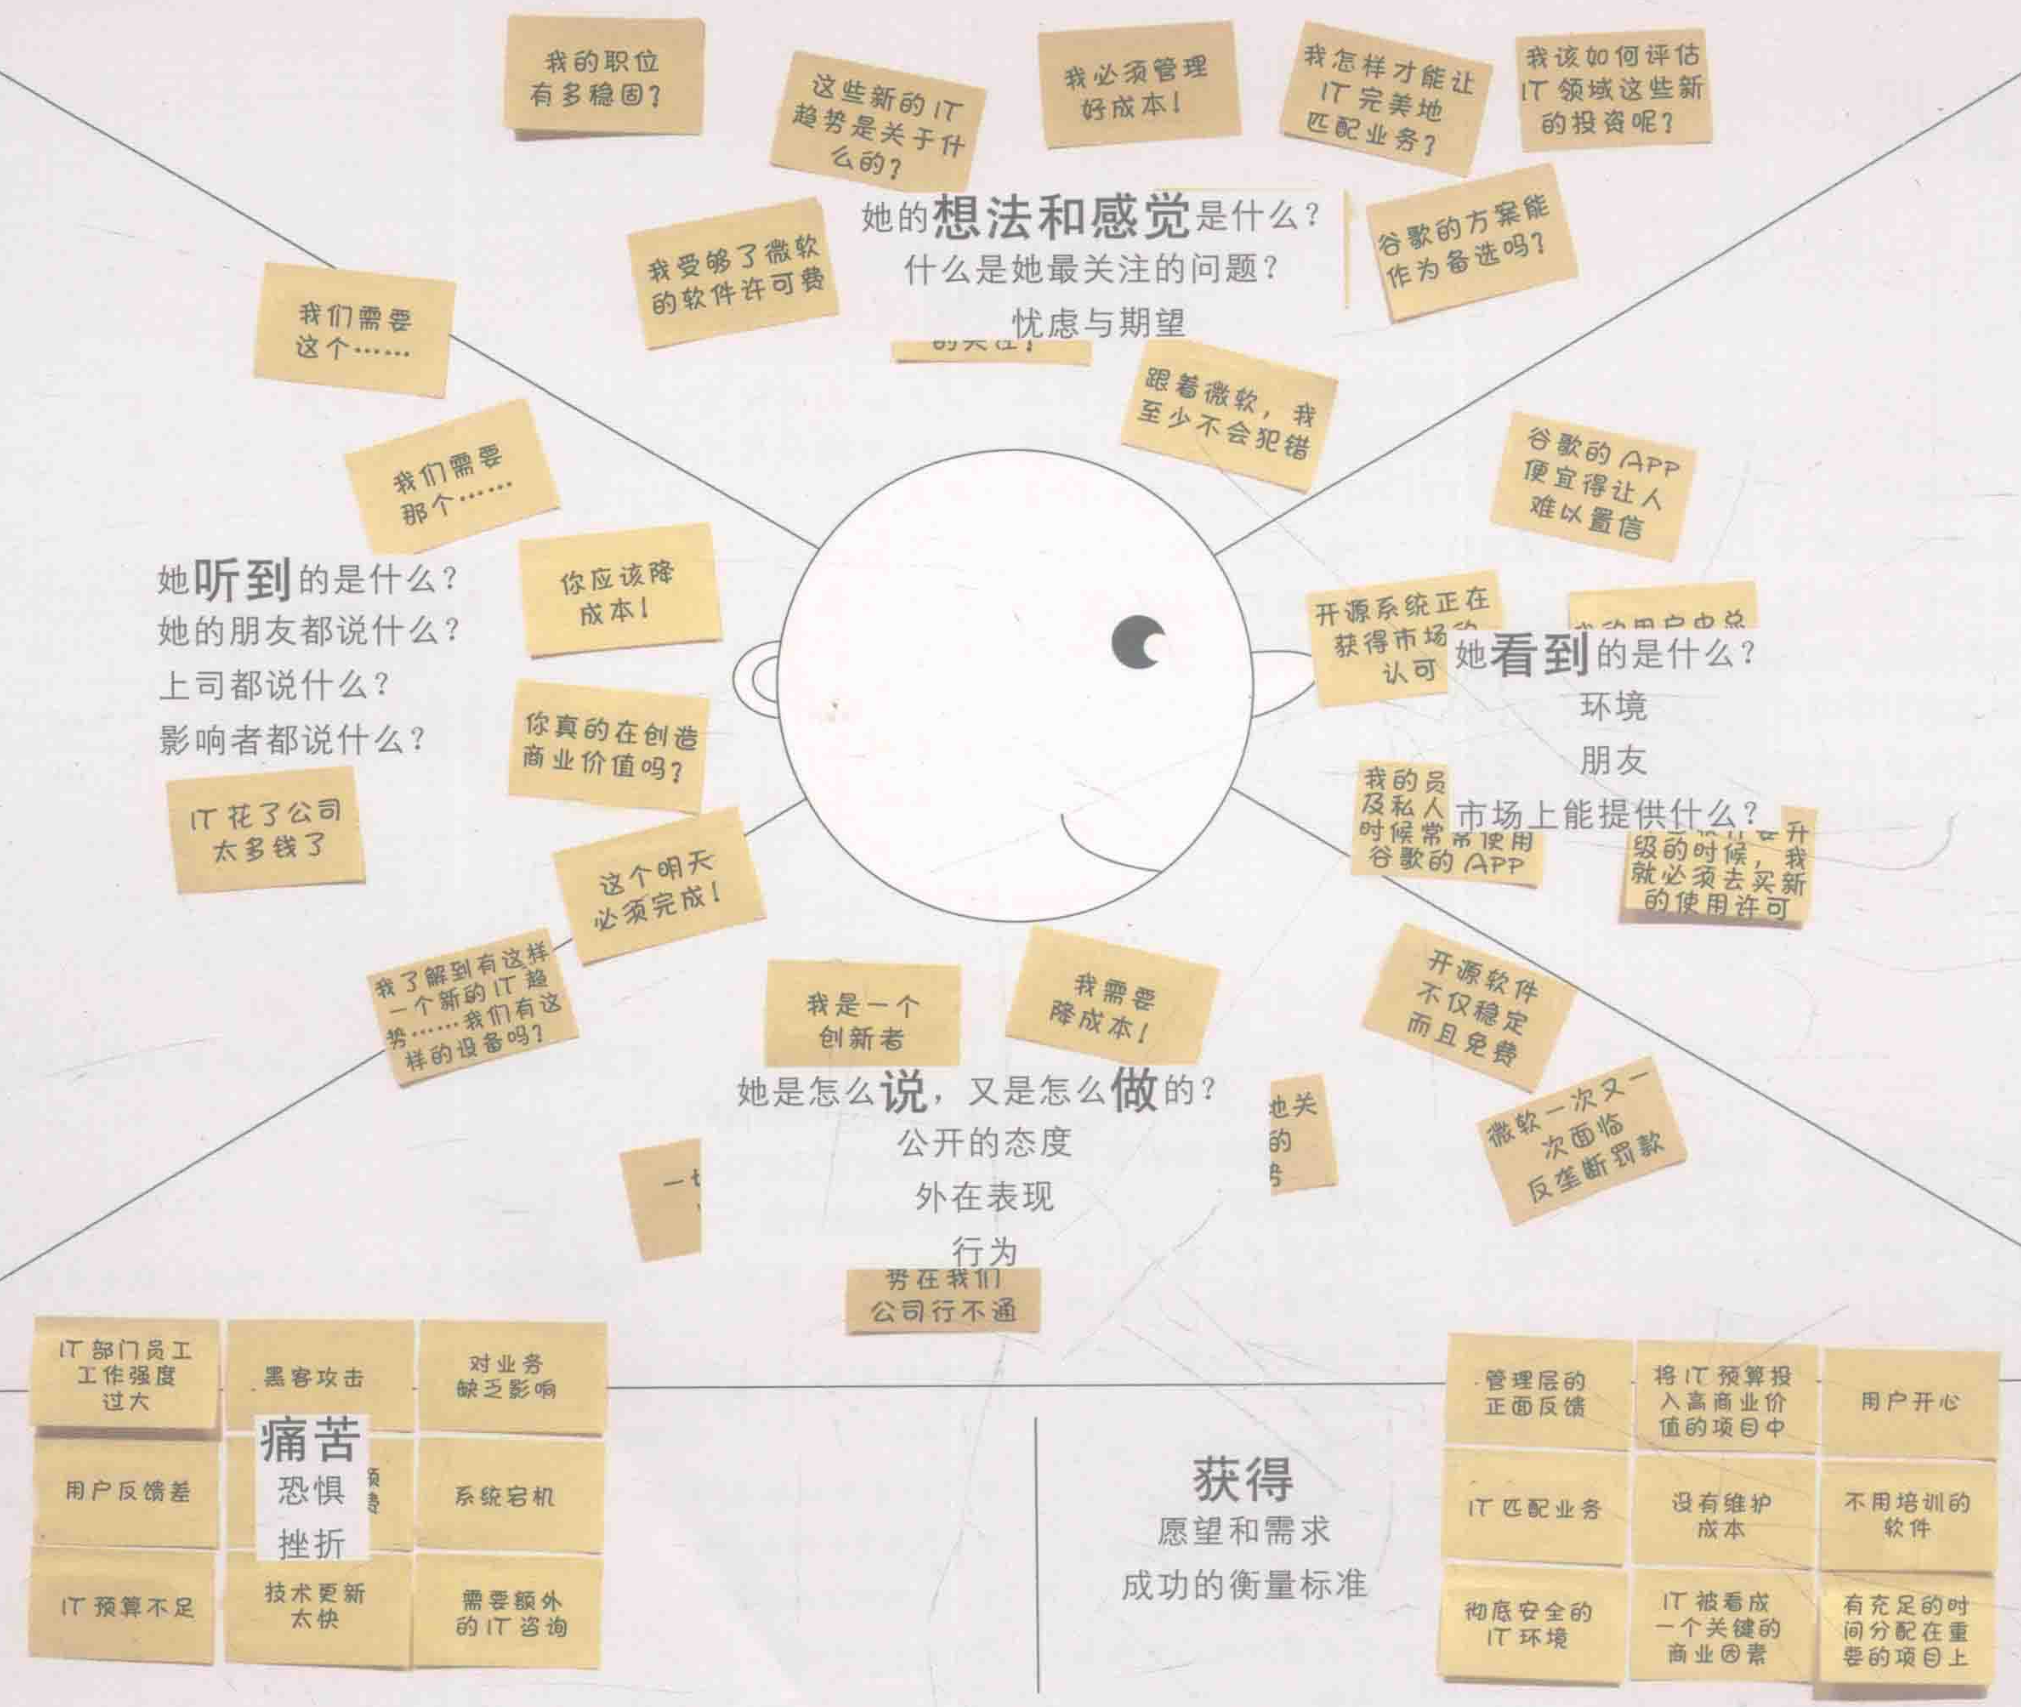
\includegraphics[width=0.8\textwidth]{img/移情图示例.png}
    \vspace{-0.5em}
\end{figure}


\subsection{构思}

通过一个创造性的流程来产生大量的商业模式创意,并且能成功地识别出最佳的创意。这个流程就被称为构思。
\begin{itemize}
    \item 构思的过程有两个主要阶段:
    \begin{itemize}
        \item 生成创意,这个阶段数量是重点
        \item 整合创意,这个阶段要把创意进行讨论、合并组合并甄选出少数可行的创意
    \end{itemize}
    \item 可行的创意并不一定要是颠覆性的商业模式。它们也可以是通过扩展你当前商业模式的领域来提升你的竞争力,这也是一种创新。
    \item 关注两点:在商业模式画布中你的商业模式创新的焦点和“如果……会怎样”的问题。
\end{itemize}

\subsubsection{商业模式创新的焦点}
\begin{itemize}
    \item 商业模式创新如果按照创新的焦点来分类,大致有4种:资源驱动、供给驱动、客户驱动和财务驱动。
    \item 这4个焦点中任何一个都可以作为重大商业模式变革的起点,也都有力地影响商业模式九宫格中的其他8个模块。
    \item 有些时候,商业模式创新可能会源自多个焦点。
    \item SWOT分析不失为一个好的工具来帮助我们找到变革的起点,它能够帮助企业深入解剖某个南业模式的优势、劣势、机会和威胁。
\end{itemize}

\begin{figure}[H]
	\centering
	\vspace{-0.5em}
	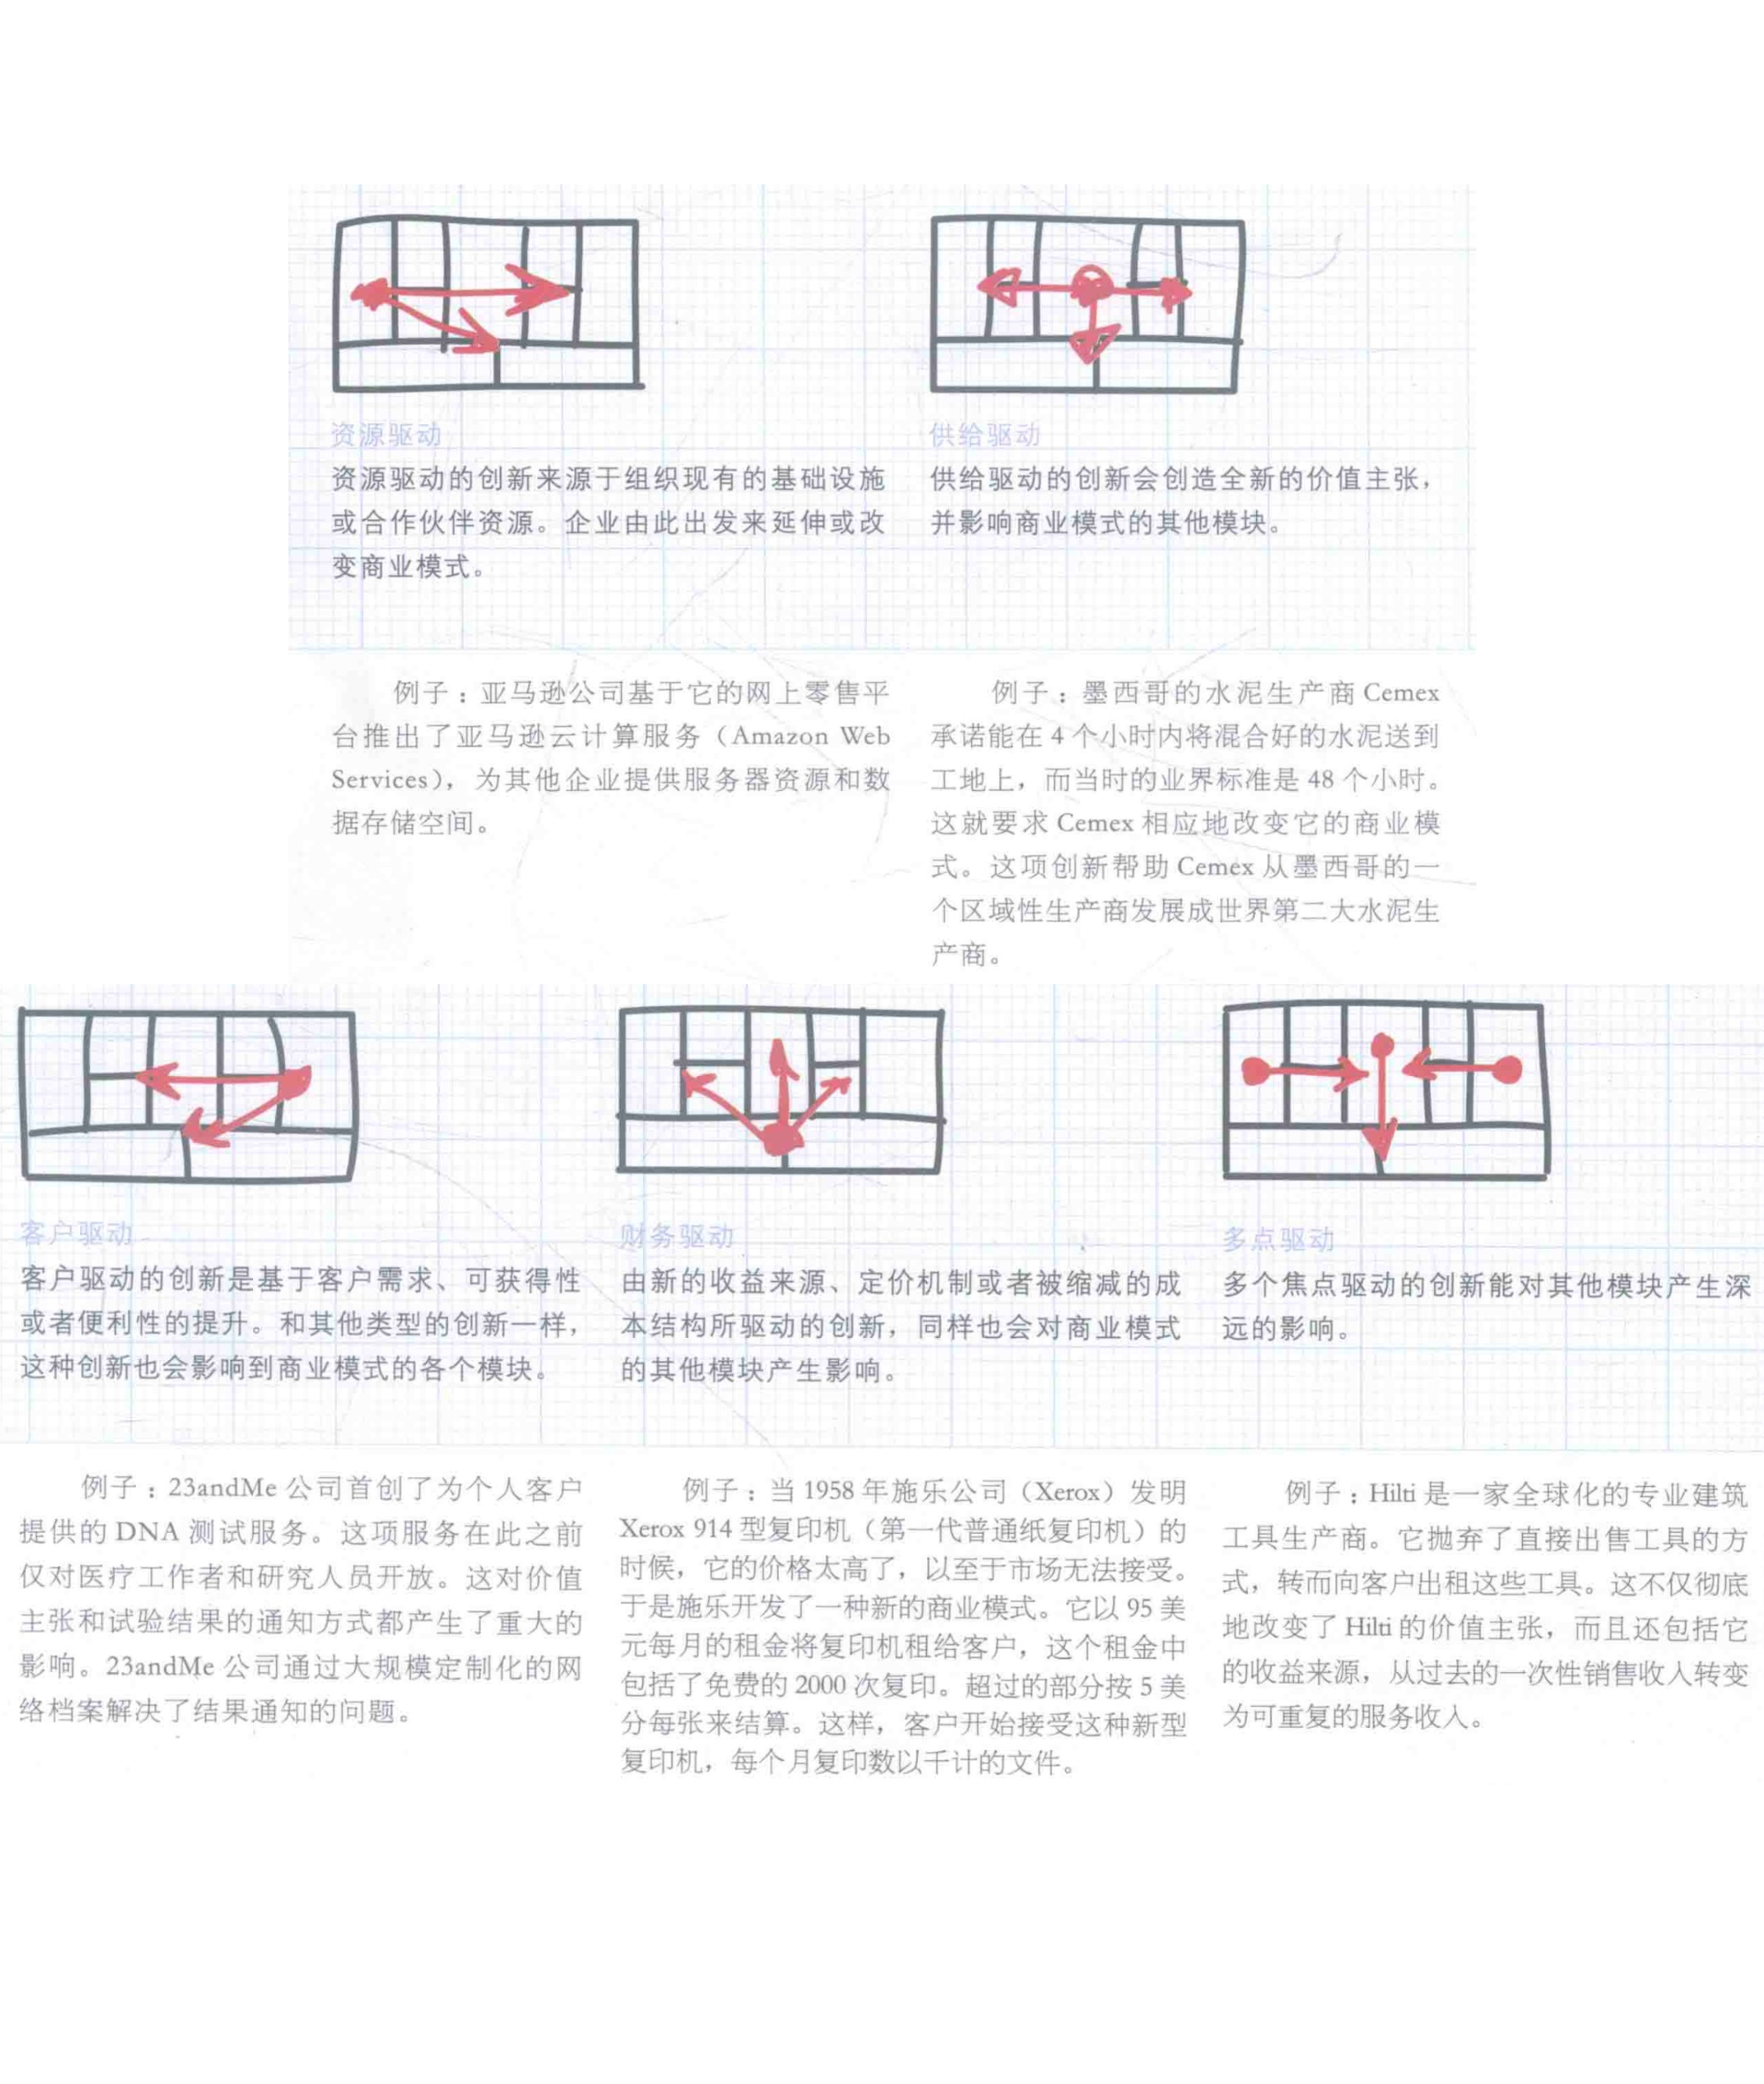
\includegraphics[width=0.9\textwidth]{img/商业模式创新的焦点.pdf}
    \vspace{-0.5em}
\end{figure}

\subsubsection{问题“如果……会怎样”的魔力}

受制于现状对思维的束缚,我们常常会苦于无法构思出创新的商业模式,现状遏制了想象力。
\begin{itemize}
    \item 克服这一问题的一个方法就是用“如果……会怎样”的问题来挑战传统假设。
    \item 有了正确的商业模式原料,一些原本认为不可能的事情也可以成为能够做到的事情。
    \item “如果……会怎样”的问题帮助我们挣脱现有商业模式的束缚。它们能激发我们,挑战我们的思维。它们还能让更多新奇的、难于执行的主张闯入我们的思维。
\end{itemize}

\subsubsection{构思的流程}
构思的流程可以采取很多种形式。这里给出的是一个能产生创新商业模式的总体方法:
\begin{enumerate}[label=\arabic*.]
    \item 团队组建:为了产生新颖的商业模式创意,我们的团队是否足够多样化?
    
    组建正确的团队对产生有效的新商业模式创意至关重要。团队成员的资历、年龄、经验水平、业务领域、客户知识和专业技能都要多样化。
    \item 钻研:在生成商业模式创意之前,我们必须钻研哪些知识?
    
    理想的团队必须经过钻研的阶段。这可能会包括总体研究、研究客户或潜在客户、详细调查新技术和评估现有的商业模式。钻研的过程可能会长达数周或短至一两次工具分析(比如移情图)。
    \item 开拓:我们能针对商业模式的每个模块做哪些创新?
    
    在这个阶段,团队尽可能地开拓解决方案的范围,以产生尽可能多的创意。商业模式九个模块中的任何一个都可以作为创新的起点。这个阶段的目的是数量,而非质量。使用头脑风暴的组织原则能让人们聚焦发掘创意,避免过早地评论创意的价值。
    \item 甄选标准:我们为商业模式创意排序最重要的标准是什么?
    
    在从最大范围上开拓了足能多的解决方案后,团队必须确定一个标准来从海量的创意中挑出数量在可管理范围内的少数创意。这个标准必须针对你的业务背景,同时还要涵盖诸如下内容:预期实施时间、潜在收入,可能的客户阻力和对竞争优势的影响。
    \item 构建模型:对于每一个进入短名单的创意,它完整的商业模式会是怎样的?
    
    标准一旦确立,团队必须有能力从若干创意中整理出一个最优创意的短名单,由此来构建$3\sim 5$个创新的商业模式。然后使用商业模式画布来勾勒和讨论每个商业模式模型。
\end{enumerate}

\subsubsection{组建一个多样化的团队}

\begin{itemize}
    \item 商业模式创新不应该仅仅限于研发或战略规划部门。
    \item 商业模式创新团队必须拥有多样化背景的团队成员。这种多样化会有助于你创造、讨论和甄选新的创意。你也可以添加一些外部人士,甚至儿童也是可以的。
    \item 多样化是有好处的。但你一定要保证能教会他们如何积极地倾听,并且考虑在关键会议上引入一个中立的引导员。
\end{itemize}

\subsubsection{头脑风暴的规则}

\begin{itemize}
    \item 保持聚焦:首先要精确地表达当前的问题。在理想情况下,这必须和客户需求有关。不要让讨论跑题太远,始终将讨论拉回到开始的问题上来。
    \item 执行规则:在一开始就闸明头脑风暴的规则并且坚决执行。其中最重要的规则是“不要过早下结论”、“每次一个人讲,不要七嘴八舌”、“追求数量”、“视觉化”和“鼓励疯狂的创意”。引导员必须执行好这些规则。
    \item 视觉化思考:把创意写下来或者画在每个人都能看到的地方。有一个搜集创意的好办法是把它们写在便利贴上, 然后贴到一面墙上。这样你可以随意地移动这些创意并将它们重新组合。
    \item 准备:通过对当前问题进行钻研来为头脑风暴做好准备。这些钻研活动可以是团队的一次实地考察以及与客户的讨论等任何形式的对你的问题陈述的钻研活动。
\end{itemize}


\subsection{视觉化思考}

\subsubsection{视觉化思考的价值}

\begin{itemize}
    \item 商业模式其实是一个内部元素相互影响的整体系统;它只有在形成一个整体的时候才是有意义的。不将它视觉化很难一目了然地抓住它的主旨。
    \item 视觉化能够一目了然的刻画商业模式的主旨,并具象化其中的隐含假设。
    \item 视觉化能够使商业模式变的明确,为团队讨论提供一些概念性的锚点,使讨论从抽象思维落实到具体、形象的东西。
    \item  视觉化既能找出已有模式中的逻辑缺陷,又能在设计全新模式时更容易地添加、删除和移动相关的图片化概念。
\end{itemize}

视觉化思考使用的两项技术与四个流程
\begin{itemize}
    \item 如何使用便利贴和如何将草图与商业模式画布结合
    \item 视觉化思考的四个流程:理解、对话、探索、沟通
\end{itemize}

\subsubsection{视觉化的实现:便利贴+绘画}
便利贴的重要性:可以随意地添加、移除,以及在商业模式各模块之间挪动
\begin{itemize}
    \item 三个简要的指导方针:用粗的马克笔、每张便利贴只写一项元素、每张便利贴上只用很少的字来抓住关键点
    \item 在用便利贴呈现的最终商业模式图景前的讨论过程和结果同样重要。参与者会讨论在画布上贴上哪张纸、移除哪张纸,辩论某项元素如何影响其他元素。
    \item 这些讨论过程都让参与者能深入地理解该商业模式和它的动态变化过程。最终,这些便利 贴就不仅仅代表了商业模式中的某个模块,它们引导了战略讨论的方向。   
\end{itemize}

绘画的强大表现力:人对图像的反应要比文字强烈的多
\begin{itemize}
    \item 最简陋的素描也能让事物变得具体和易于理解:如情绪、比例等。
    \item 帮助向别人解释和沟通你的商业模式,容易激发起建设性的讨论与创意。
    \item 可用于勾勒一个典型客户与他所处的环境,也可用于勾勒出客户群体的需求和任务。
\end{itemize}

\subsubsection{视觉化的作用}
\begin{itemize}
    \item 理解商业模式的本质
    \begin{itemize}
        \item 视觉化的语言:画布是一张概念图,其功能类似于具有语法规则的视觉化语言,提供了视觉和文字的指引,帮助画出模式中所需的所有信息
        \item 抓住全貌:画布的草图能够为观众提供足够的信息理解全貌,而不被过多的细节影响理解
        \item 看到关键:一定要理解元素/模块之间的关联关系
    \end{itemize}
    \item 提升对话效率
    \begin{itemize}
        \item 共同的参照点:将头脑中不言而喻的主观假设具象化,并将大量内容固化成为可回溯的参照点(人类的短时记忆只能保留有限数量的想法)
        \item 统一的语言:利用图形和画布帮助不同参与者聚焦,特别是来自不同领域的人
        \item 一致的理解:帮助不同部门的人将其深入理解的部分表达出来,再一起形成整体的洞察与一致的理解
    \end{itemize}
    \item 探索创意
    \begin{itemize}
        \item 激发创意:模糊的想法—随着灵感发挥—有机地整合成一幅图画
        \item 演习:视觉化的模型帮助思考部分元素的改变引发的系统性冲击
    \end{itemize}
    \item 提升沟通
    \begin{itemize}
        \item 统一公司内部的理解:用图画在组织内形成共识,朝一个战略方向前进
        \item 内部推销:好的图画使组织的现状、需要做的事情、怎么做、未来会怎样等方面变得易于沟通,从而赢得组织内部的理解和支撑
        \item 外部推销:提升向投资人或潜在合作伙伴推销成功的概率 
    \end{itemize}
\end{itemize}

\subsubsection{为不同的需求采取不同的视觉化方式}
根据目标的不同,视觉化的商业模式需要展示出不同程度的细节。例如Skype的商业模式就直观地展现了它与传统电信运营商的关键区别。它的目标在于指出Skype商业模式与传统运营商的显著差异,尽管它们提供类似的服务。

\begin{figure}[H]
	\centering
	\vspace{-0.5em}
	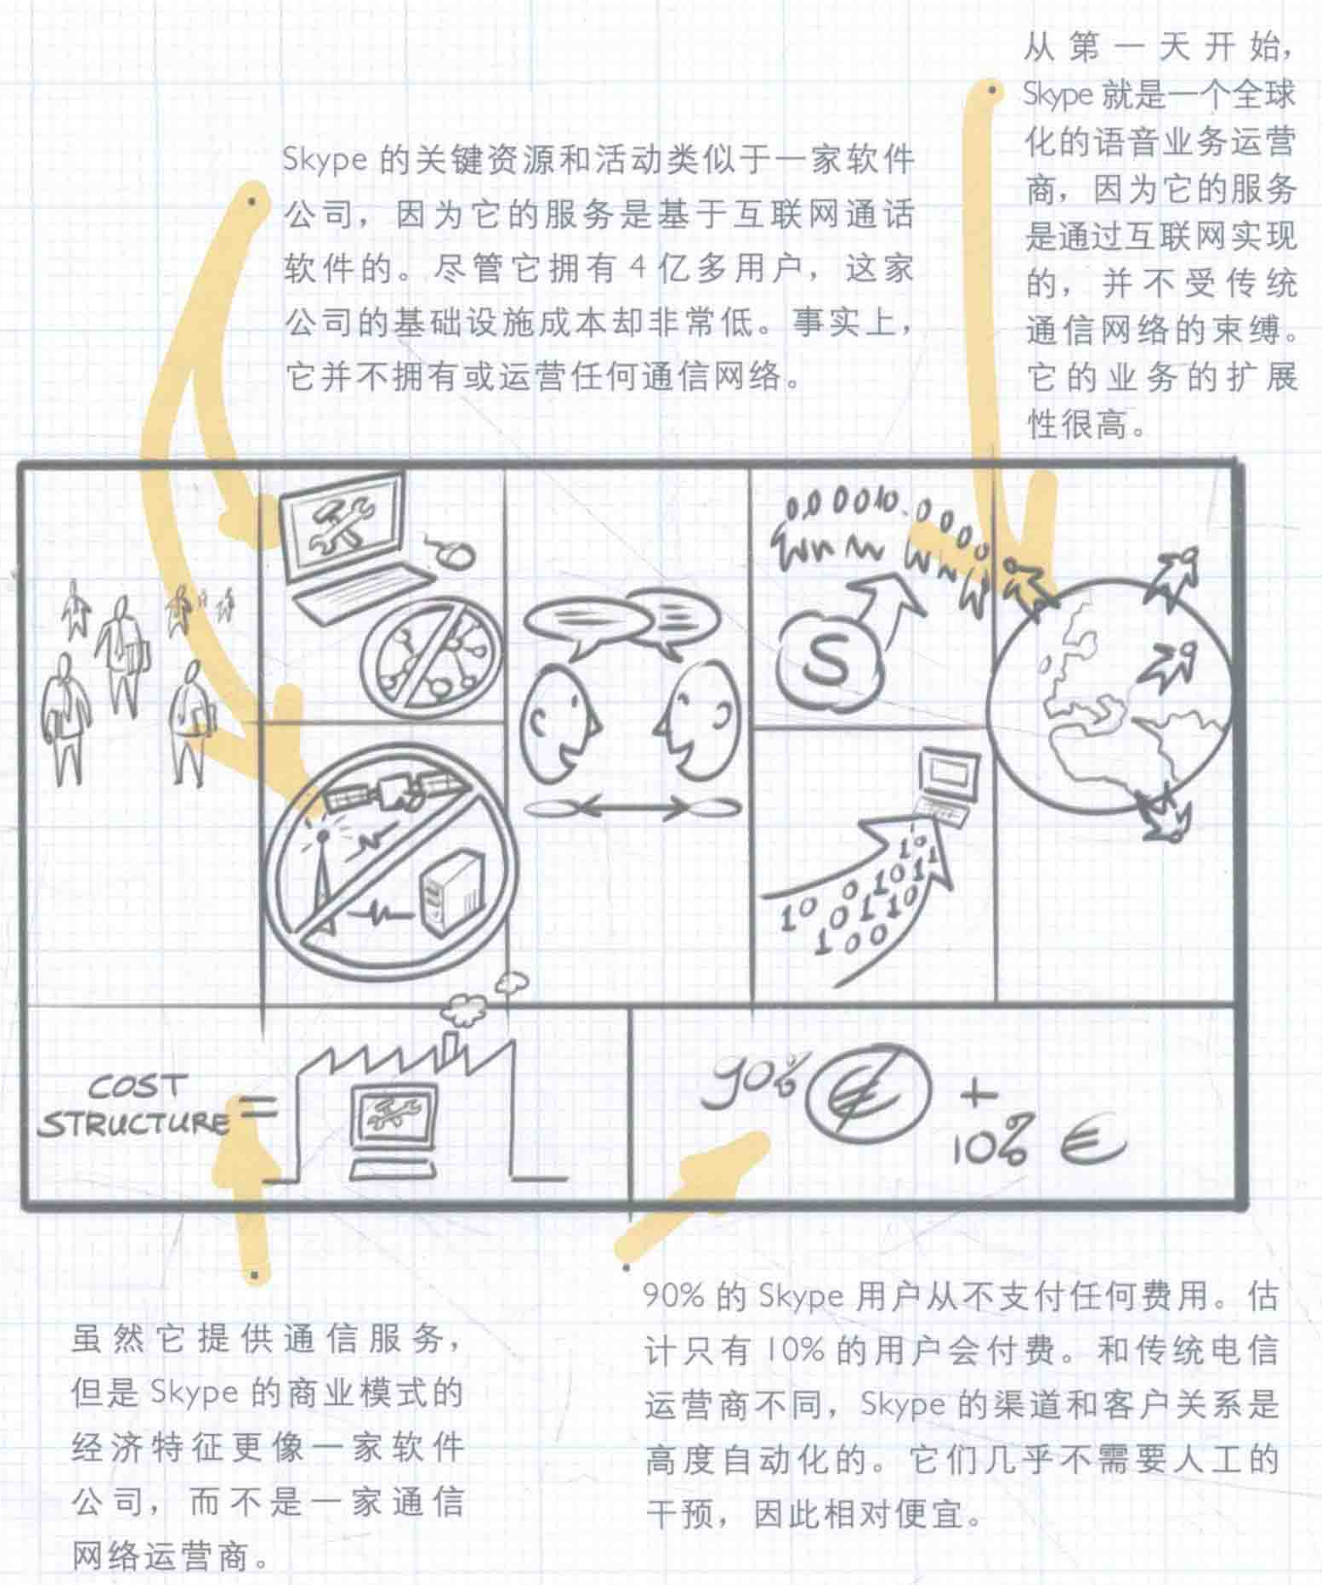
\includegraphics[width=0.6\textwidth]{img/为不同的需求采取不同的视觉化方式.png}
    \vspace{-0.5em}
\end{figure}

\subsubsection{讲述一个视觉化的故事}

解释商业模式的一种有力的方式:利用画布草图逐一介绍一个完整的视觉化故事

如何讲述视觉化故事
\begin{figure}[H]
	\centering
	\vspace{-0.5em}
	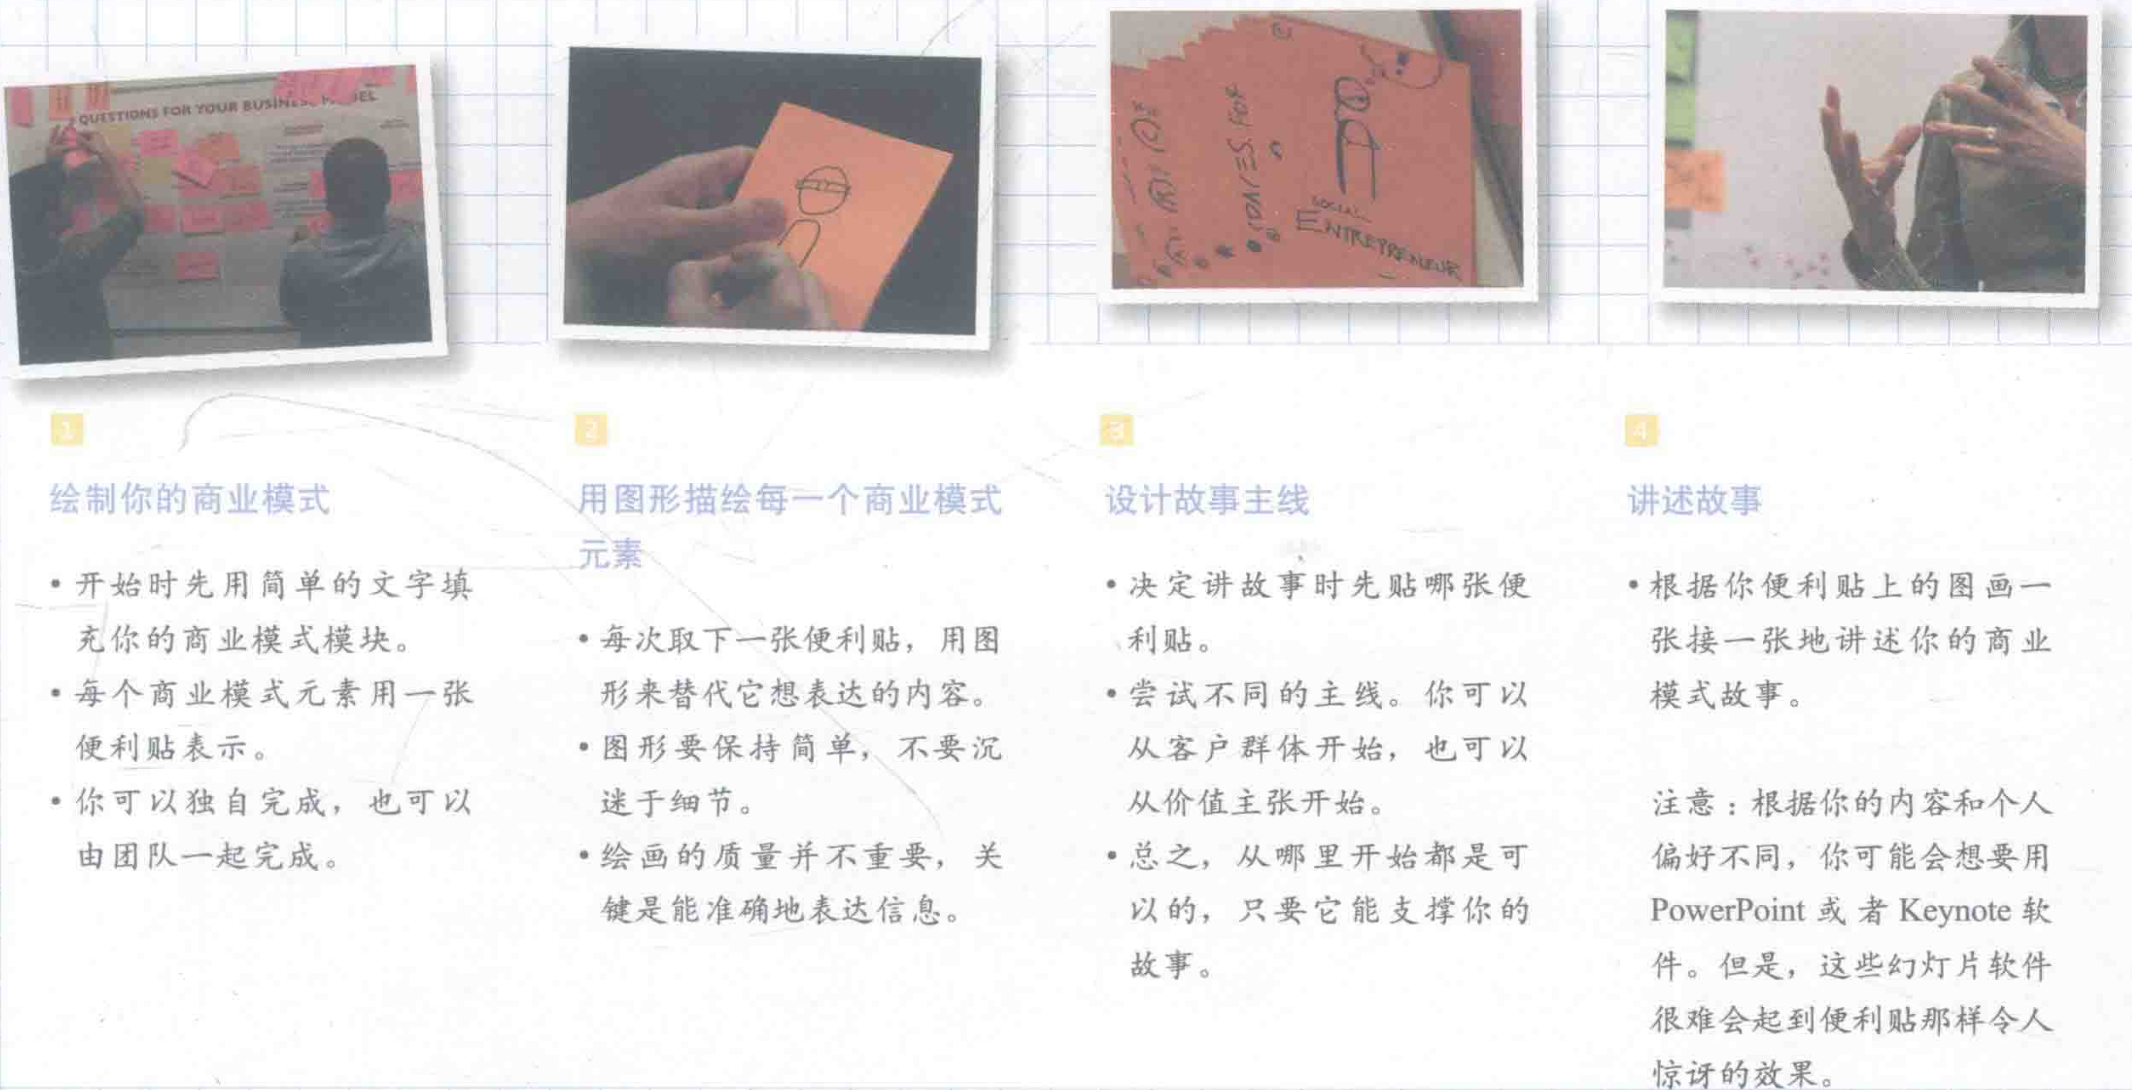
\includegraphics[width=0.9\textwidth]{img/如何讲述视觉化故事.png}
    \vspace{-0.5em}
\end{figure}

\subsection{模型构建}

\subsubsection{模型构建的价值}
模型构建是一个很有力的工具,可以开发出新颖、创新的商业模式。
\begin{itemize}
    \item 和视觉化思考一样,模型构建可以让抽象的概念具体化,有助于探索出新的创意。
    \begin{itemize}
        \item 模型构建这项技术来自设计学和工程学,被广泛地用在产品设计、架构设计和交互式设计。它在商业管理领域却不是很常用,主要是因为组织行为和战略的抽象性。
        \item 把模型看成未来潜在的商业模式:是一个用于讨论、探究或者概念验证的工具。
        \item 一个商业模式模型可以是一张简单的草图,一张充分思考过的商业模式画布,或者是一叠模拟新商业模式财务状况的数据表格。
    \end{itemize}
    \item 模型构建有助于实际商业模式的探索。
    \begin{itemize}
        \item 建模$\rightarrow$(疑问点明确化、视觉化)$\rightarrow$添加、删除或修改元素$\rightarrow$观察结果。
        \item 在不同规模(抽象层面)的模型上进行互动。
        \item 有助于获得突破性的商业模式,同时能够有效控制细节。
    \end{itemize}
\end{itemize}

\subsubsection{设计态度}
\begin{itemize}
    \item 设计态度包括了愿意去探素原始的想法,迅速地放弃这些想法,然后花时间检查多种可能性,直到选出少数值得优化的想法,而且要接受这种不确定性,直到设计方向成熟。
    \item 这些素质井不是专业人士与生俱来的,但它们是开发新的商业模式所必需的。
    \item 设计态度要求人们从做决定的思维转化为创造多种可选方案来选择的思维。
\end{itemize}

\subsubsection{构建不同规模的模型}
控制规模:通过绘制很多(粗略的和细致的)模型来代表各种战略选择,再通过对每个模型添加和移除元素的方式来探索新想法
\begin{itemize}
    \item 随手素描:勾勒和推销一个粗略的创意
    
    画一个简单的商业模式画布,仅仅用关键元素来描述这个创意
    \begin{itemize}
        \item 勾勒想法
        \item 包含价值主张
        \item 包含主要收益来源
    \end{itemize}
    \item 精心描绘的画布:探索实现该创意所需的因素
    
    通过描绘一个相对详细的面布来探索该商业模式所需的所有元素。
    \begin{itemize}
        \item 描绘整张画布
        \item 通过你的商业逻辑来思考
        \item 预估市场潜力
        \item 理解商业模式画布各个模块之间的关系
        \item 做一些基本的“事实查证”工作
    \end{itemize}
    \item 商业案例:检查该创意的可存活度
    
    将详细的画布转化为财务表格,估算你的商业模式的盈利潜力
    \begin{itemize}
        \item 建立一张全面的画布
        \item 包含关键数据
        \item 计算成本和收入
        \item 估算利润潜力
        \item 根据不同的假设进行财务场景模拟
    \end{itemize}

    \item 实地验证:调查用户的接受度和可行性
    
    你已经在一个潜在的新商业模式上下定决心,现在需要去实地验证它的某个方面。
    \begin{itemize}
        \item 为这个新商业模式准备一个合情合理的商业案例
        \item 站在客户的角度或者让真实的客户来进行实地验证
        \item 验证价值主张、渠道、定价机制等实际市场中的元素
    \end{itemize}
\end{itemize}

利用模型构建探究决策到执行的转换
\begin{figure}[H]
	\centering
	\vspace{-0.5em}
	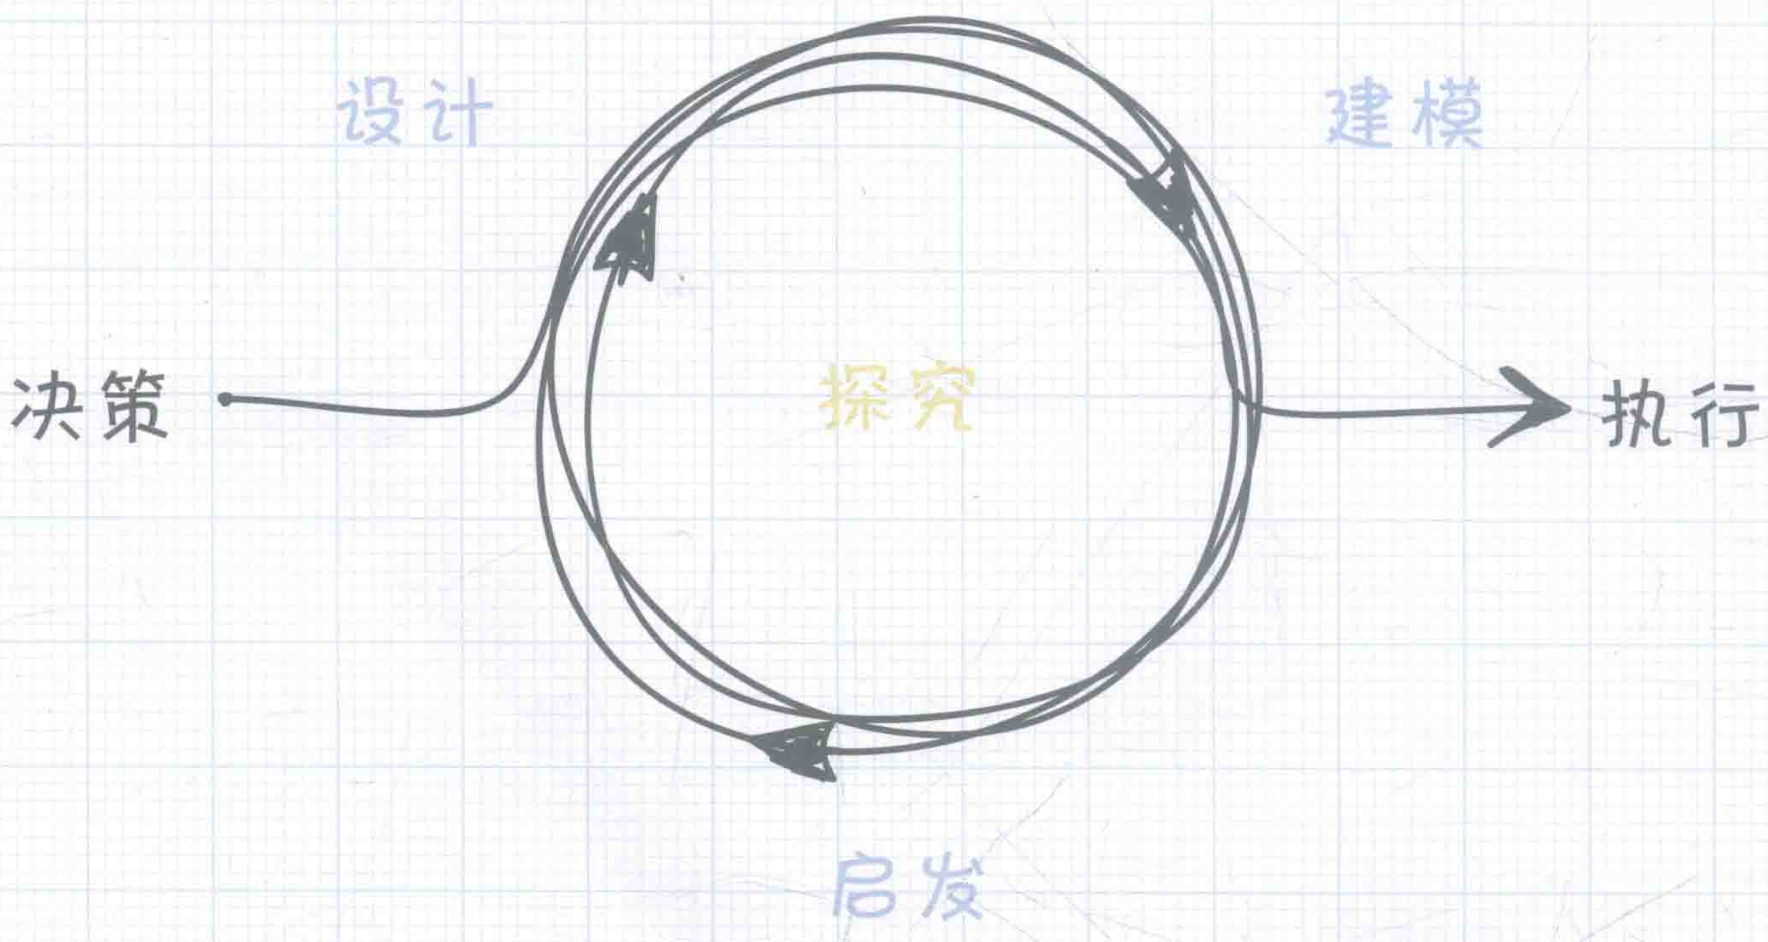
\includegraphics[width=0.5\textwidth]{img/利用模型构建探究决策到执行的转换.png}
    \vspace{-0.5em}
\end{figure}


\subsection{讲故事}

\subsubsection{讲故事的价值}
故事是一个理想的热身工具,为深度讨论商业模式与其内在逻辑做好准备
\begin{itemize}
    \item 将故事与画布结合,利用叙事性克服听众对不熟悉模式的抵触,放下对陌生事物的怀疑
\end{itemize}

为什么要讲故事
\begin{itemize}
    \item 介绍新想法:尝试融入组织战略
    \item 向投资人推销:争取外部资源
    \item 吸引员工:抓住组员的注意力和好奇心,为下一步探讨准备
    \item 让未来触手可及:激发创意、辩证变革
\end{itemize}

\subsubsection{故事的不同视角}
\begin{figure}[H]
	\centering
	\vspace{-0.5em}
	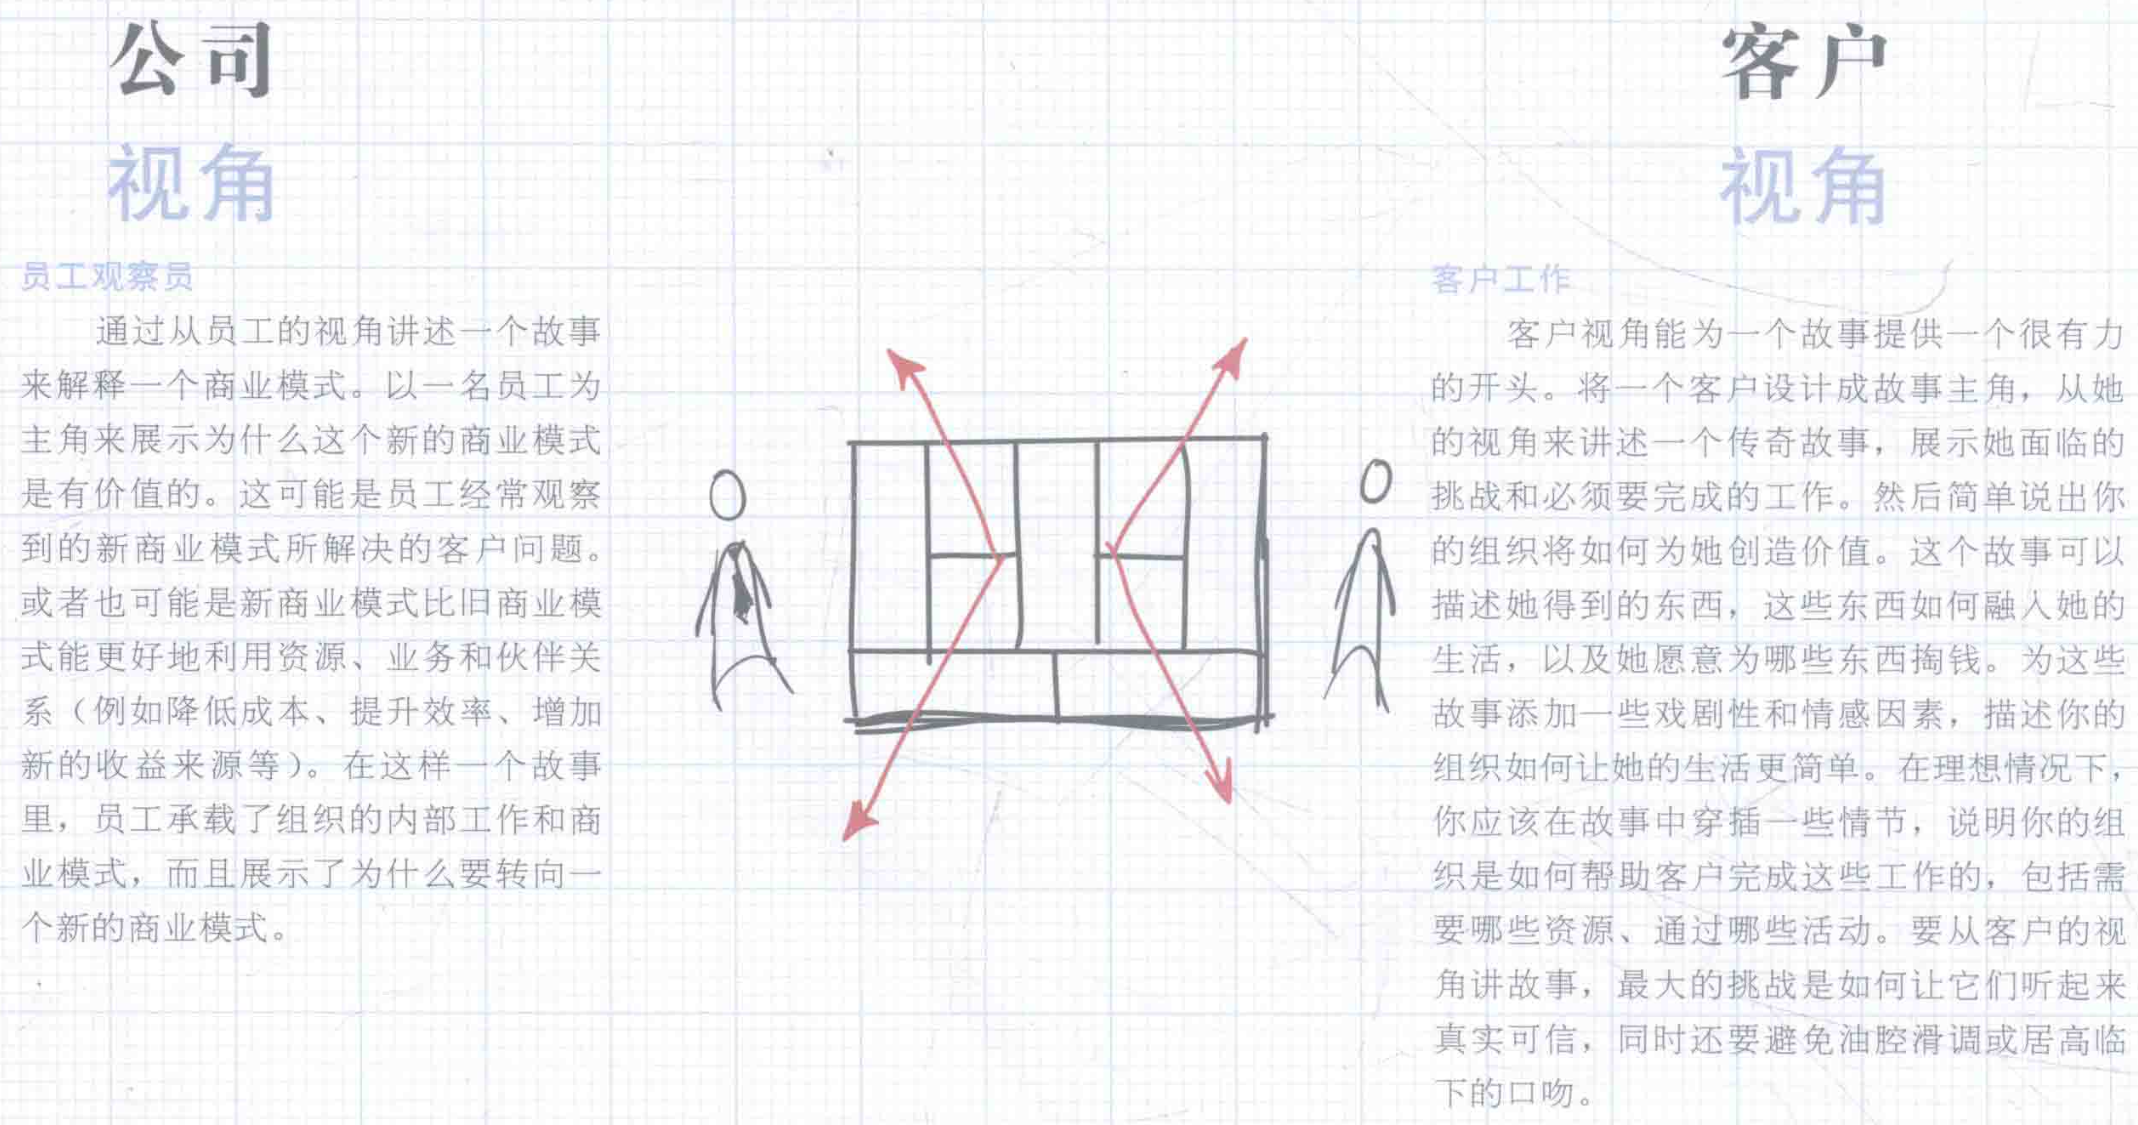
\includegraphics[width=0.7\textwidth]{img/故事的不同视角.png}
    \vspace{-0.5em}
\end{figure}

\subsubsection{讲故事的方法}

\begin{table}[H]
    \centering
    \resizebox{\textwidth}{!}{
        \begin{tabular}{|l|l|l|l|l|l|}
            \hline
                  & 图片和旁白                                                                  & 视频                                                                                & 角色扮演                                                                & 文字和图片                                                                   & 连环图画                                                                   \\ \hline
            描述    & \begin{tabular}[c]{@{}l@{}}用一张或很多张图片来\\ 讲述一个主角的故事和\\ 他的环境\end{tabular} & \begin{tabular}[c]{@{}l@{}}用视频来讲述一个主角\\ 的故事和他的环境可以\\ 拉近现实与幻想之间的\\ 距离\end{tabular} & \begin{tabular}[c]{@{}l@{}}让人们扮演故事中的主\\ 角,构建逼真形象的场\\ 景\end{tabular} & \begin{tabular}[c]{@{}l@{}}用文字和一到数张图片\\ 来讲述一个主角的故事\\ 及他的环境\end{tabular} & \begin{tabular}[c]{@{}l@{}}用一系列的卡通图片来\\ 栩栩如生地讲述一个主\\ 角的故事\end{tabular} \\ \hline
            何时用?  & 小组讨论或会场讲演                                                              & \begin{tabular}[c]{@{}l@{}}向一大群听众广播或者\\ 内部做有重要财务意义\\ 的决策\end{tabular}             & \begin{tabular}[c]{@{}l@{}}相互陈述新开发的商业\\ 模式创意的研讨会\end{tabular}       & \begin{tabular}[c]{@{}l@{}}向一大群听众汇报或广\\ 播\end{tabular}                  & \begin{tabular}[c]{@{}l@{}}向一大群听众汇报或广\\ 播\end{tabular}                 \\ \hline
            时间和成本 & 低                                                                      & 中/高                                                                               & 低                                                                   & 低                                                                       & 低/中                                                                    \\ \hline
            \end{tabular}
    }
    \end{table}


\subsection{场景}

场景能够很好地指导新商业模式的设计或者对当前商业模式的创新。场景也能让抽象的事物变得具体。
\begin{itemize}
    \item 不同的客户结构:产品或服务将被如何使用,什么样的客户会用到它们,客户的担忧、诉求和目标。
    \begin{itemize}
        \item 这些场景是基于客户洞察,但通过融入我们对客户的理解描绘出了独特、具体的图景。
        \item 通过描述具体的环境,客户场景能将客户洞察变得栩栩如生。
    \end{itemize}
    \item 商业模式未来可能的竞争环境:这里的目的不是为了预测未来,而是为了想象未来可能的具体细节。
    \begin{itemize}
        \item 这样能让创新者仔细体会未来各种环境下最合适的商业模式。
        \item 将场景规划的方法用到商业模式创新领域能让人品味到特定条件下商业模式会如何演进。
        \item 这能加深对商业模式及其必要调整措施的理解。更重要的是,它能够帮助我们对未来做好准备。
    \end{itemize}
\end{itemize}

将场景融入商业模式创新活动
\begin{figure}[H]
	\centering
	\vspace{-0.5em}
	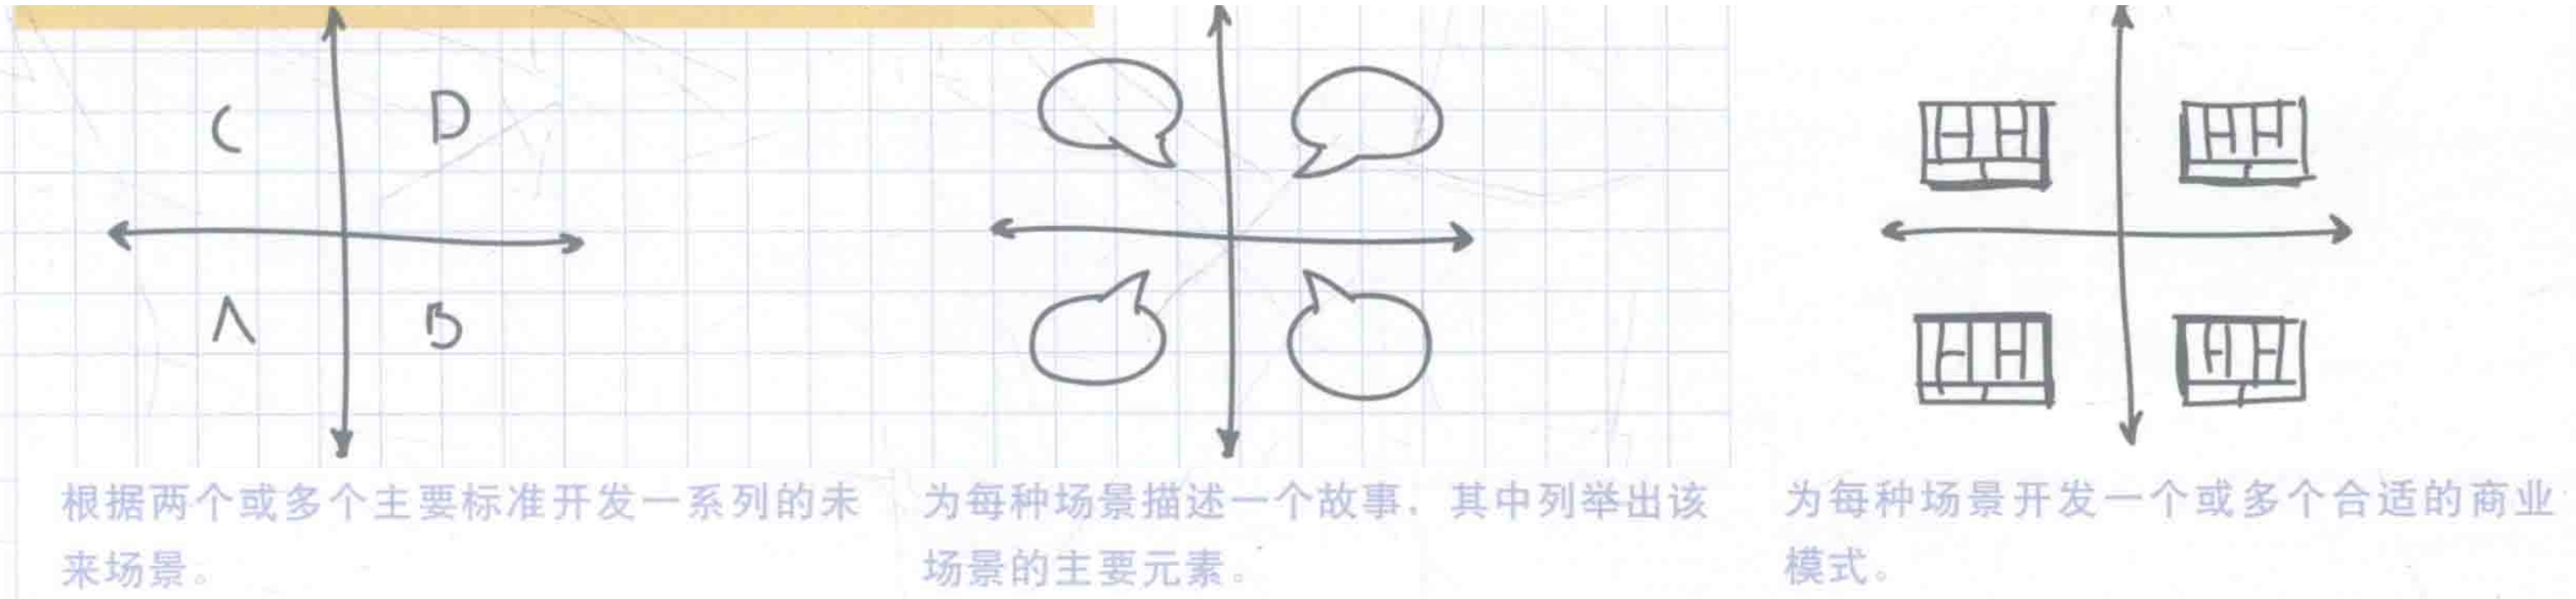
\includegraphics[width=0.8\textwidth]{img/将场景融入商业模式创新活动.png}
    \vspace{-0.5em}
\end{figure}

例:未来的医药商业模式
\begin{figure}[H]
	\centering
	\vspace{-0.5em}
	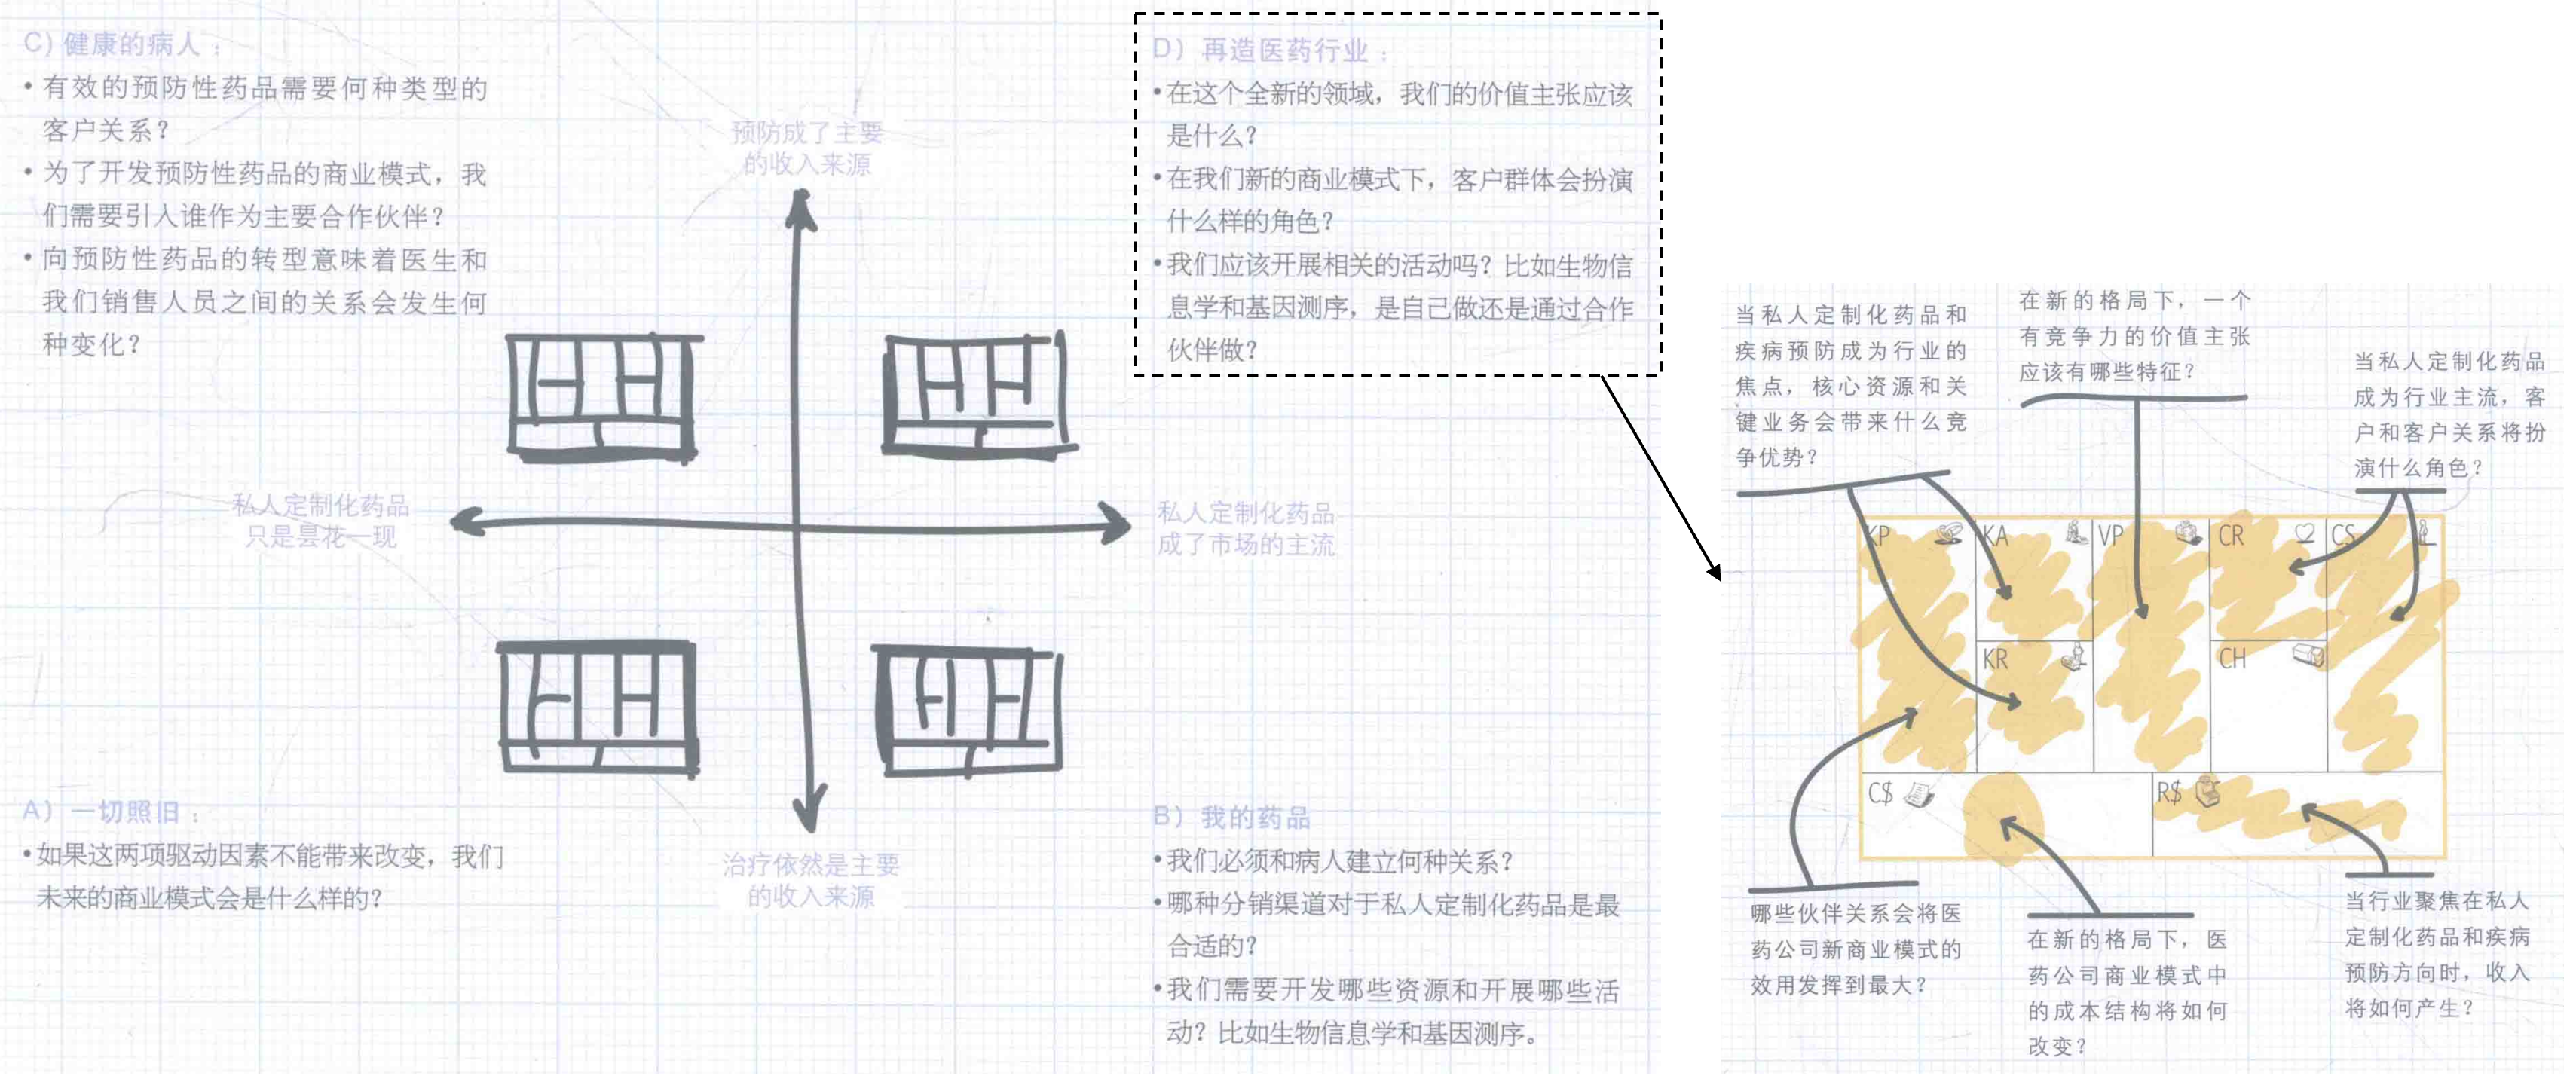
\includegraphics[width=\textwidth]{img/未来的医药商业模式.png}
    \vspace{-0.5em}
\end{figure}



	\section{商业模式战略}

商业模式战略领域:\textbf{商业模式环境}、\textbf{评估商业模式}、从商业模式的视角看\textbf{蓝海战略}的商业模式解读,以及如何在企业内部\textbf{管理多种商业模式}。

\subsection{商业模式环境}

日益复杂的经济环境(比如网络商业模式)、更大的不确定性(比如技术创新)和严峻的市场颠覆(比如经济动荡、颠覆性的新价值主张),这些都使得不断地审视环境比以前任何时候都重要。理解环境中的这些变化能帮助你把商业模式调整得更有效地化解外部力量。

\begin{figure}[H]
	\centering
	\vspace{-0.5em}
	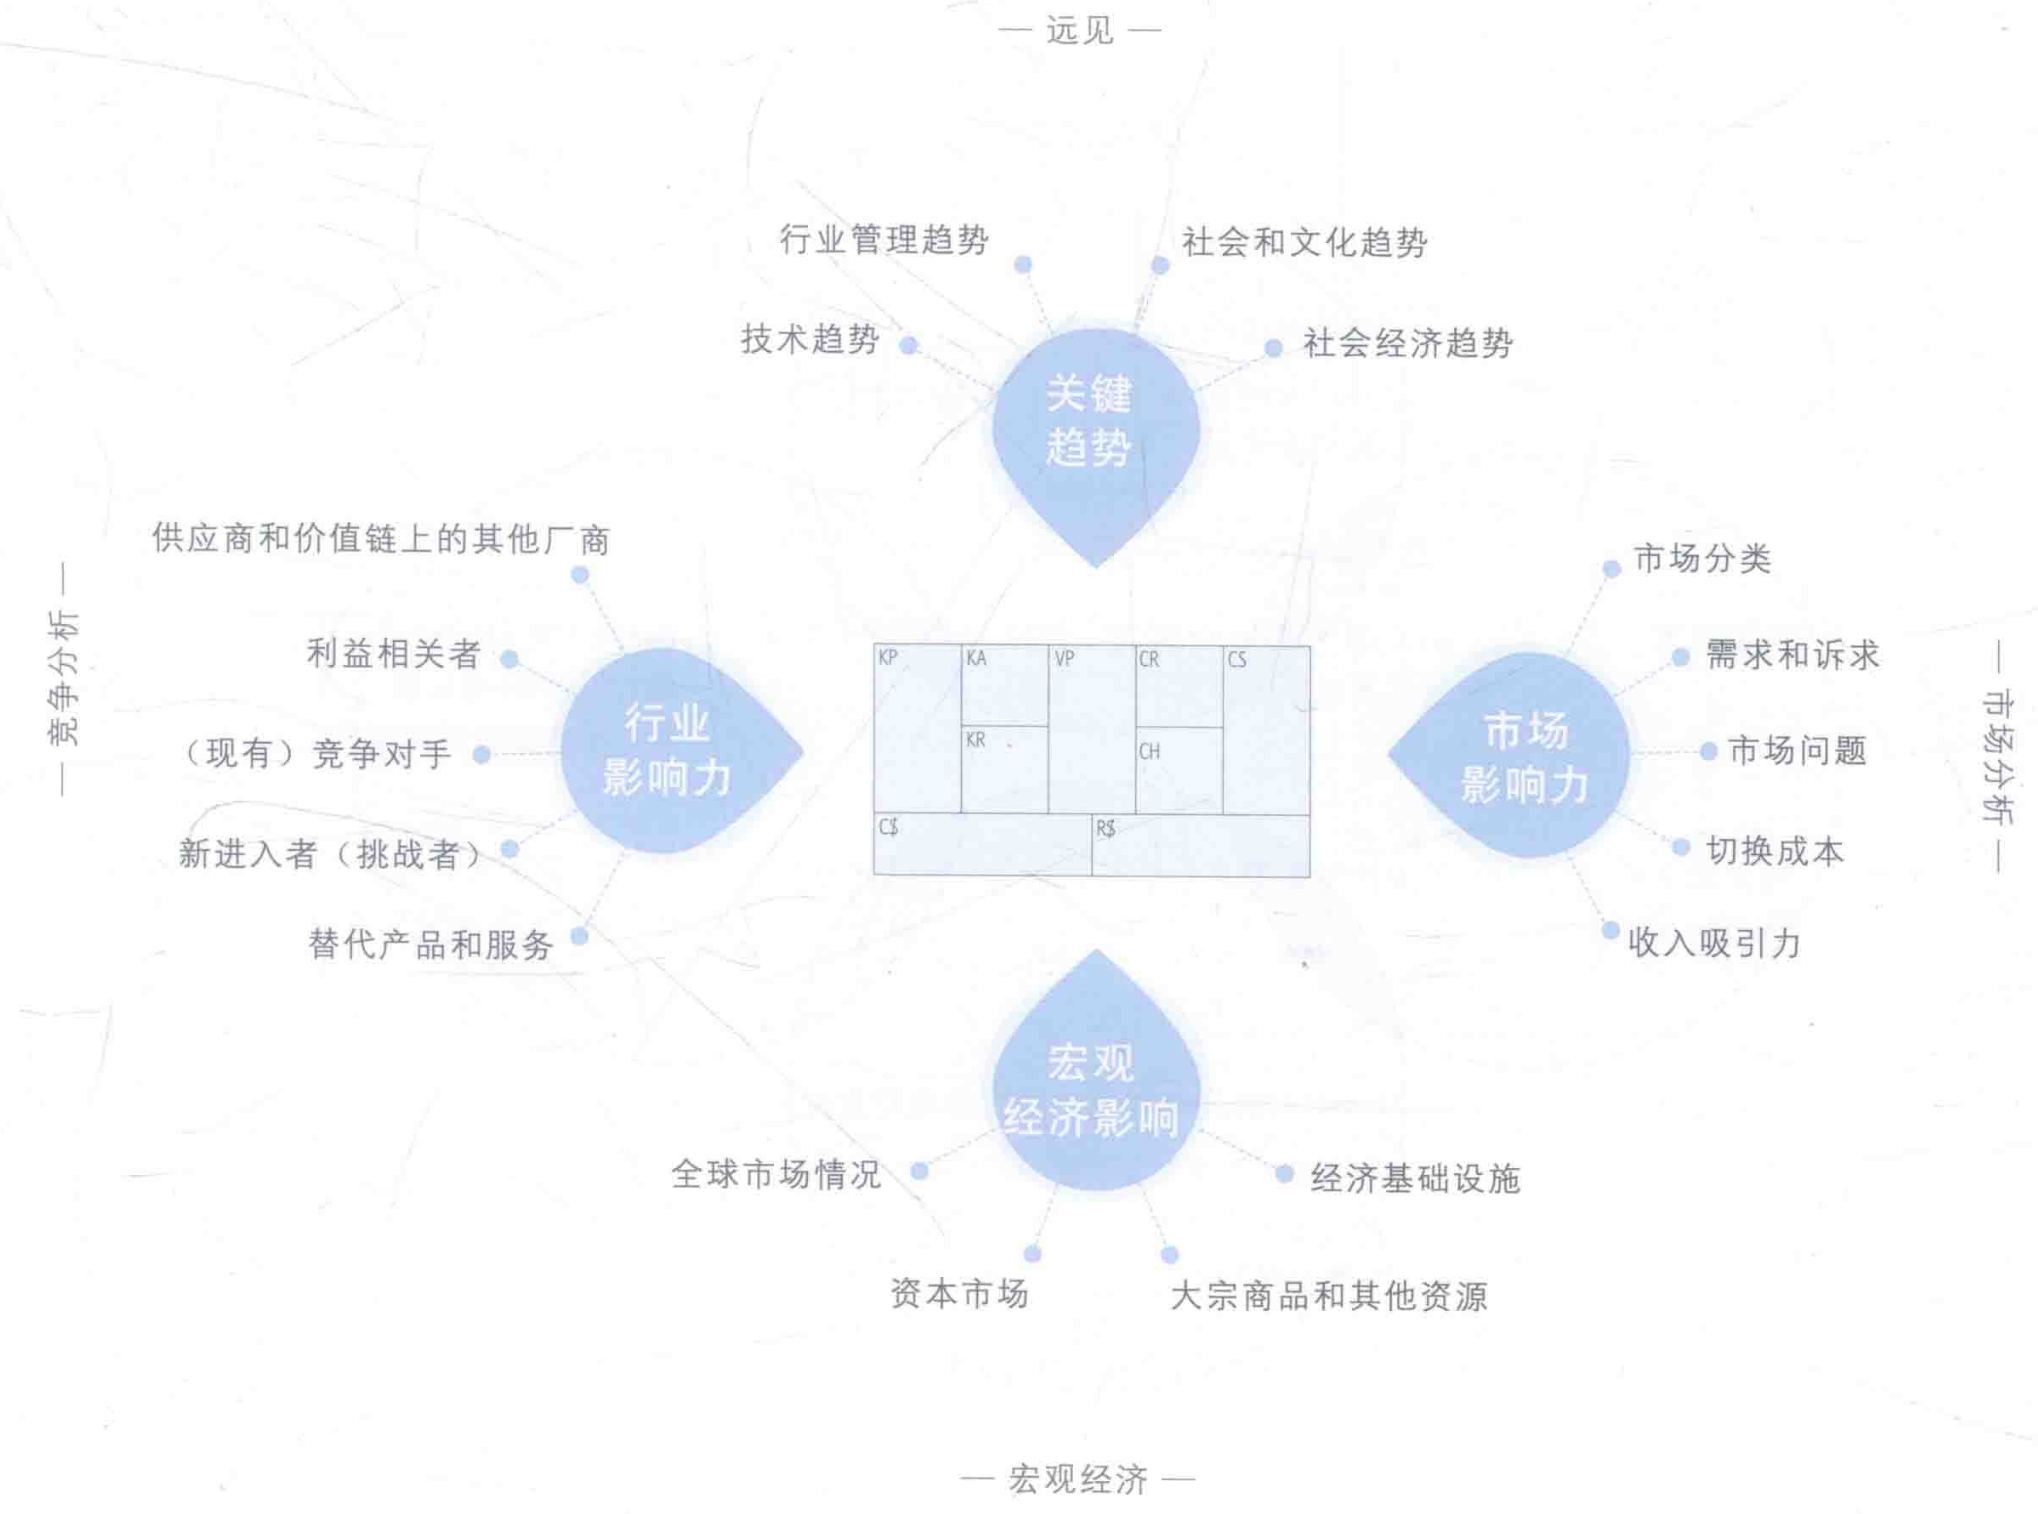
\includegraphics[width=0.8\textwidth]{img/商业模式环境评估.png}
    \vspace{-0.5em}
\end{figure}

\subsection{评估商业模式}

和年度体检一样,定期评估商业模式是一项重要的管理活动。这能让一个组织评估它的市场地位的健康程度,并且做出相应的调整。这种检查将成为商业模式不断进步的基础 ,或者也可能触发一次颠覆性的商业模式创新。
\begin{itemize}
    \item 某商业模式的总体评估,以及相应的未来战略
    \item 商业模式优势、劣势、机会和威胁(Strength, Weakness, Opportunity, Threat, SWOT)的检查清单(Checklist)
\end{itemize}

例:亚马逊总体商业模式评估
\begin{figure}[H]
	\centering
	\vspace{-0.5em}
	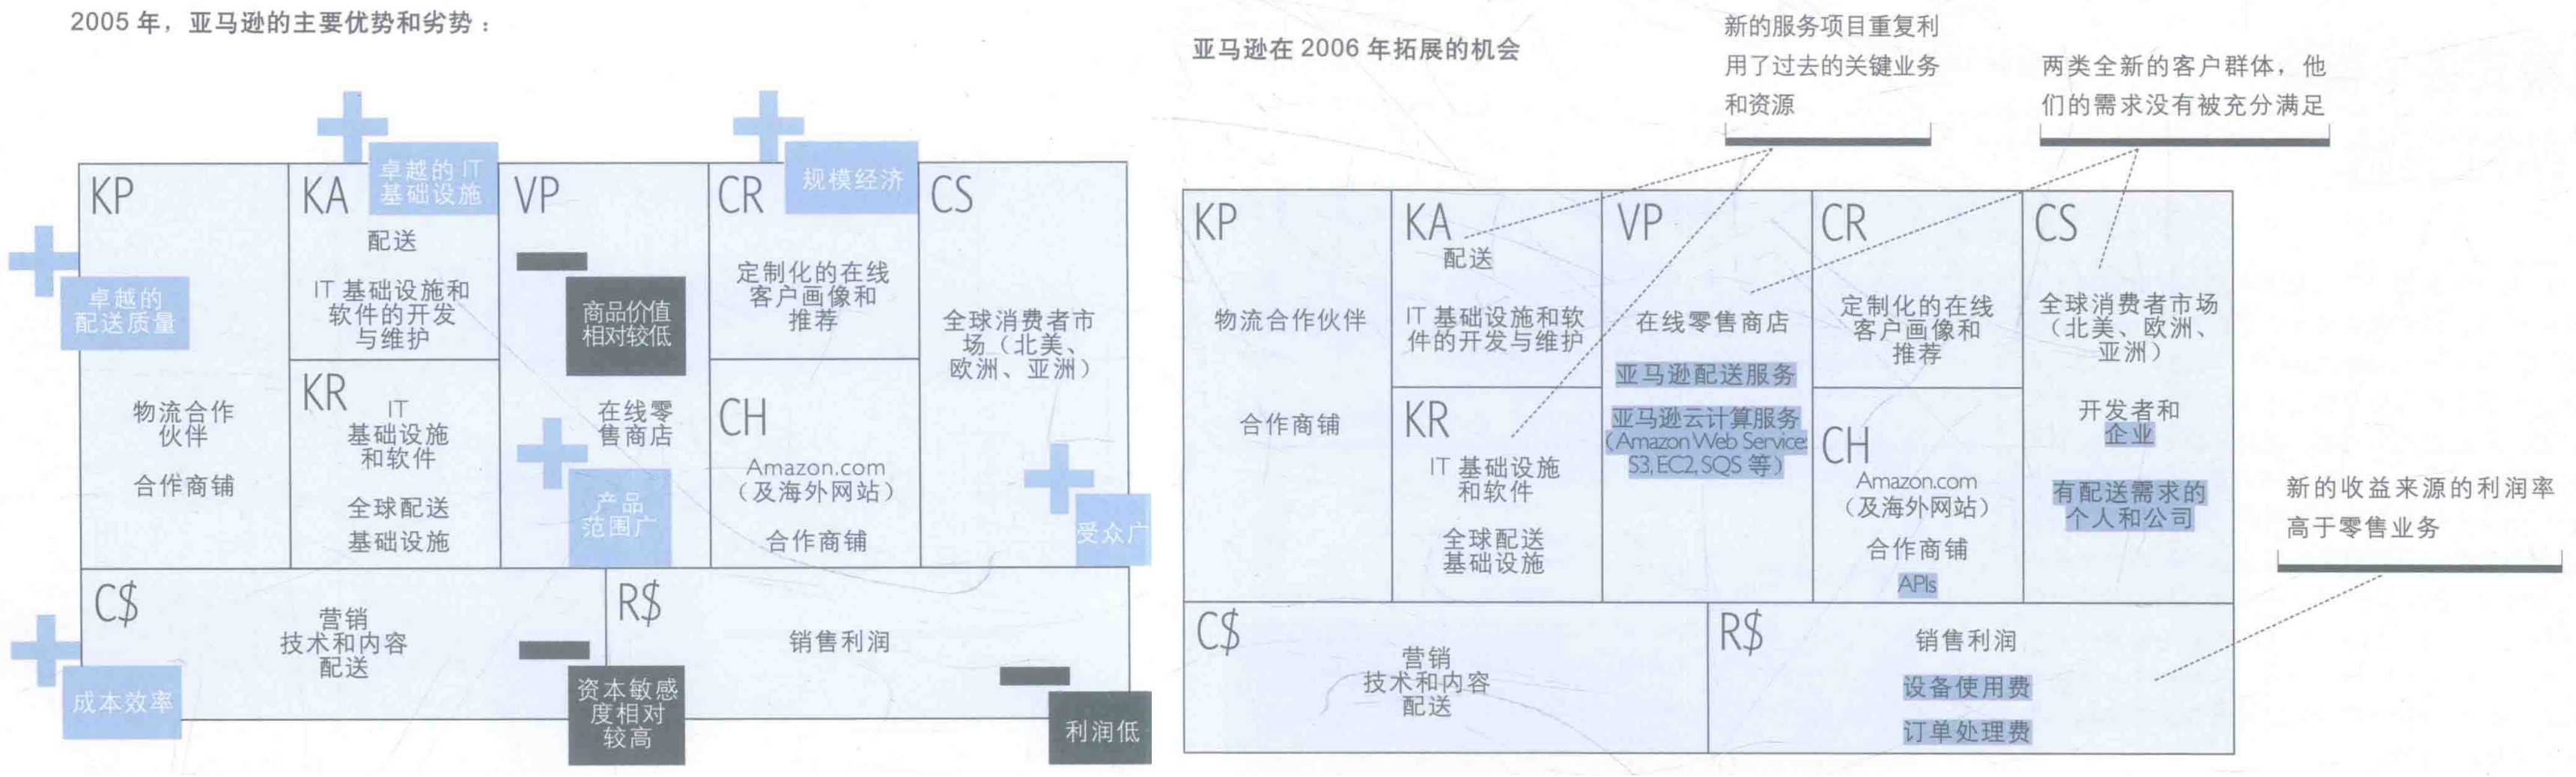
\includegraphics[width=\textwidth]{img/亚马逊总体商业模式评估.png}
    \vspace{-0.5em}
\end{figure}

对商业模式每个模块进行SWOT评估
\begin{itemize}
    \item SWOT分析是用来分析一个组织的优势和劣势,识别潜在的机会与威胁的工具。
    \item  SWOT问了四个简单的大问题。前两个——你的组织的优势和劣势是什么?内部评估你的组织。后两个——你的组织的机会有哪些,面临的潜在威胁又有哪些?在所处的环境下评估你的组织的位置。
\end{itemize}
\begin{figure}[H]
	\centering
	\vspace{-0.5em}
	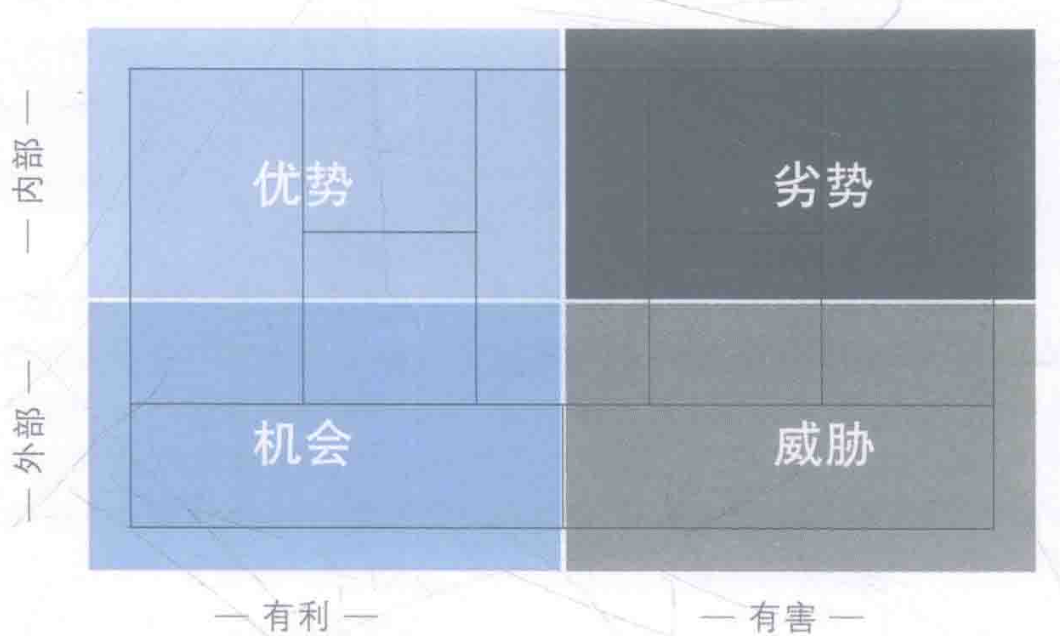
\includegraphics[width=0.5\textwidth]{img/SWOT评估.png}
    \vspace{-0.5em}
\end{figure}

优势劣势(SW)评估
\begin{multicols}{2}
\begin{itemize}
    \item 价值主张评估
    \begin{itemize}
        \item 我们的价值主张与客户需求一致
        \item 我们的价值主张具有很强的网络效应
        \item 在我们的产品和服务之间有很强的协同效应
        \item 我们的客户非常满意
    \end{itemize}
    \item 成本/收入评估
    \begin{itemize}
        \item 我们有较高的利润率
        \item 我们的收益是可预测的
        \item 我们有很多经常性收入,有很多回头客
        \item 我们的收入来源是多样化的
        \item 我们的收入来源是可持续的
        \item 我们在支出成本之前就有收入进账
        \item 客户真正想买的就是我们提供的
        \item 我们的定价机制可以抓住客户全部的购买意愿
        \item 我们的成本是可预测的
        \item 我们的成本结构与商业模式是完全匹配的
        \item 我们的运营低成本、高效率
        \item 我们受益于规模效应
    \end{itemize}
    \item 基础设施评估
    \begin{itemize}
        \item 竞争对手很难复制我们的核心资源
        \item 我们的资源需求是可预测的
        \item 我们在恰当的时间合理的调配核心资源
        \item 我们高效的执行了关键业务
        \item 我们的关键业务很难被复制
        \item 我们的执行质量很高
        \item 我们很好的平衡了自主业务和外包业务
        \item 我们专心致志,并且在必要的时候与合作伙伴合作
        \item 我们和重要合作伙伴的工作关系十分融洽
    \end{itemize}
    \item 客户界面评估
    \begin{itemize}
        \item 我们的客户的流失率很低
        \item 我们很好的细分了客户群体
        \item 我们不断的获得新的客户
        \item 我们的渠道通路很有效率
        \item 我们的渠道通路设置合理
        \item 我们的渠道通路与客户群是强接触的
        \item 我们的客户很容易就能看到我们的渠道通路
        \item 我们的渠道通路被高度整合
        \item 我们的渠道通路创造出了范围效应
        \item 我们的渠道通路很好的匹配了客户群体
        \item 我们有良好的客户关系
        \item 我们的客户关系品质与客户群体相匹配
        \item 客户切换的成本很高,客户与我们绑定了关系
        \item 我们的品牌很强
    \end{itemize}
\end{itemize}
\end{multicols}


评估机会(O)
\begin{itemize}
    \item 价值主张中的机会(整合、服务化与拓展)
    \begin{itemize}
        \item VP:产品与服务能否整合,产品能否服务化?价值主张的补充和外延?满足客户的额外需求或其它可做的工作?
    \end{itemize}
    \item 成本/收入中的机会(可重复、交叉销售、开源节流)
    \begin{itemize}
        \item  R\$:重复性收入代替一次性收入、寻找额外买单元素与交叉销售的机会、新的收益来源、能否提价
        \begin{itemize}
            \item 交叉销售:通过客户关系管理发现现有顾客的多种需求,并通过满足其需求而销售多种相关服务或产品的一种新兴营销方式
        \end{itemize}
        \item C\$:成本削减
    \end{itemize}
    \item 基础设施中的机会(强化核心、减轻负担、转让闲置)
    \begin{itemize}
        \item KR:核心资源的降本、外包、强化、转让
        \item KA:标准化、IT技术带来的整体效率提升
        \item KP:外包与核心业务聚焦、交叉销售与更好的客户连接、价值主张补充
    \end{itemize}
    \item 客户界面的机会(增长的市场、客户细分、渠道优化与去中间商,客户关系加强与取舍)
    \begin{itemize}
        \item CS:找到增长的市场并从中获利、服务新客户群体或更细致的已有客户分类
        \item CH:渠道的效率、效益、整合,补充性的渠道伙伴,去中间商、渠道客户匹配
        \item CR:加强与客户的关系并提升客户跟进的效果、定制化或可自动维护、提升切换成本、是否抛弃没有利润的客户以及原因  
    \end{itemize}
\end{itemize}

评估威胁(T)
\begin{itemize}
    \item 对价值主张的威胁(可替代性)
    \begin{itemize}
        \item 产品是否可替代?
        \item 是否会被更有竞争力的价格或更好的价值取代?
    \end{itemize}
    \item 对成本/收入的威胁(利润的威胁、是否单一、缩水、无法预测、无法支撑)
    \begin{itemize}
        \item 受威胁的利润?是否是技术原因导致?
        \item 是否过度依赖某一项或多项收益来源?
        \item 未来可能消失(或缩水)的收益来源?
        \item 是否有无法预测的成本?
        \item 哪些成本的增加会快过它们所支撑的收入?
    \end{itemize}
    \item 对基础设施的威胁(供应不足、干扰、合作关系波动)
    \begin{itemize}
        \item KR:某些资源的供应短缺?资源的质量是否有保证?
        \item KA:哪些关键业务会被打扰?我们的活动质量能否保证?
        \item KP:可能失去的合作伙伴?是否会跟竞争对手合作?是否过分依赖某些合作伙伴?
    \end{itemize}
    \item 客户界面上的威胁(市场竞争、渠道威胁、客户关系恶化)
    \begin{itemize}
        \item CS:市场是否很快饱和?市场份额被友商威胁?客户转投的可能性?竞争白热化的速度?
        \item CH:竞争对手是否威胁渠道?是否存在渠道与客户不相关的危险?
        \item CR:我们的客户关系有可能恶化吗?
    \end{itemize}
\end{itemize}


\subsection{蓝海战略}

蓝海战略是通过根本性的差异化来创造全新的行业,而不是通过模仿现有商业模式在当前行业中竞争。
\begin{itemize}
    \item 相对于在传统的绩效指标下超越对手,更加倡导创造新的、未充分竞争的市场空间,这称之为价值创新
    \begin{itemize}
        \item 这意味着通过创造新的利益和服务来为客户增加价值,同时通过削减低价值的功能或服务来降低成本。
        \item 为了实现价值创新,提出了“四项行动架构”。以 四个关键问题可以挑战一个行业的战略逻辑和现行的商业模式:
        \begin{itemize}
            \item 行业中哪些看起来理所当然的要素应该被删除?
            \item 哪些要素应该被大幅削减到行业标准之下?
            \item 哪些要素应该大幅提升到行业标准之上?
            \item 哪些行业中从未提供的要素是应该被创造出来的?
        \end{itemize}
    \end{itemize}
    \item 除了价值创新,还建议开拓未被开发的客户群体,以此来创造蓝海和发现新的市场。
\end{itemize}

\begin{figure}[H]
	\centering
	\vspace{-0.5em}
	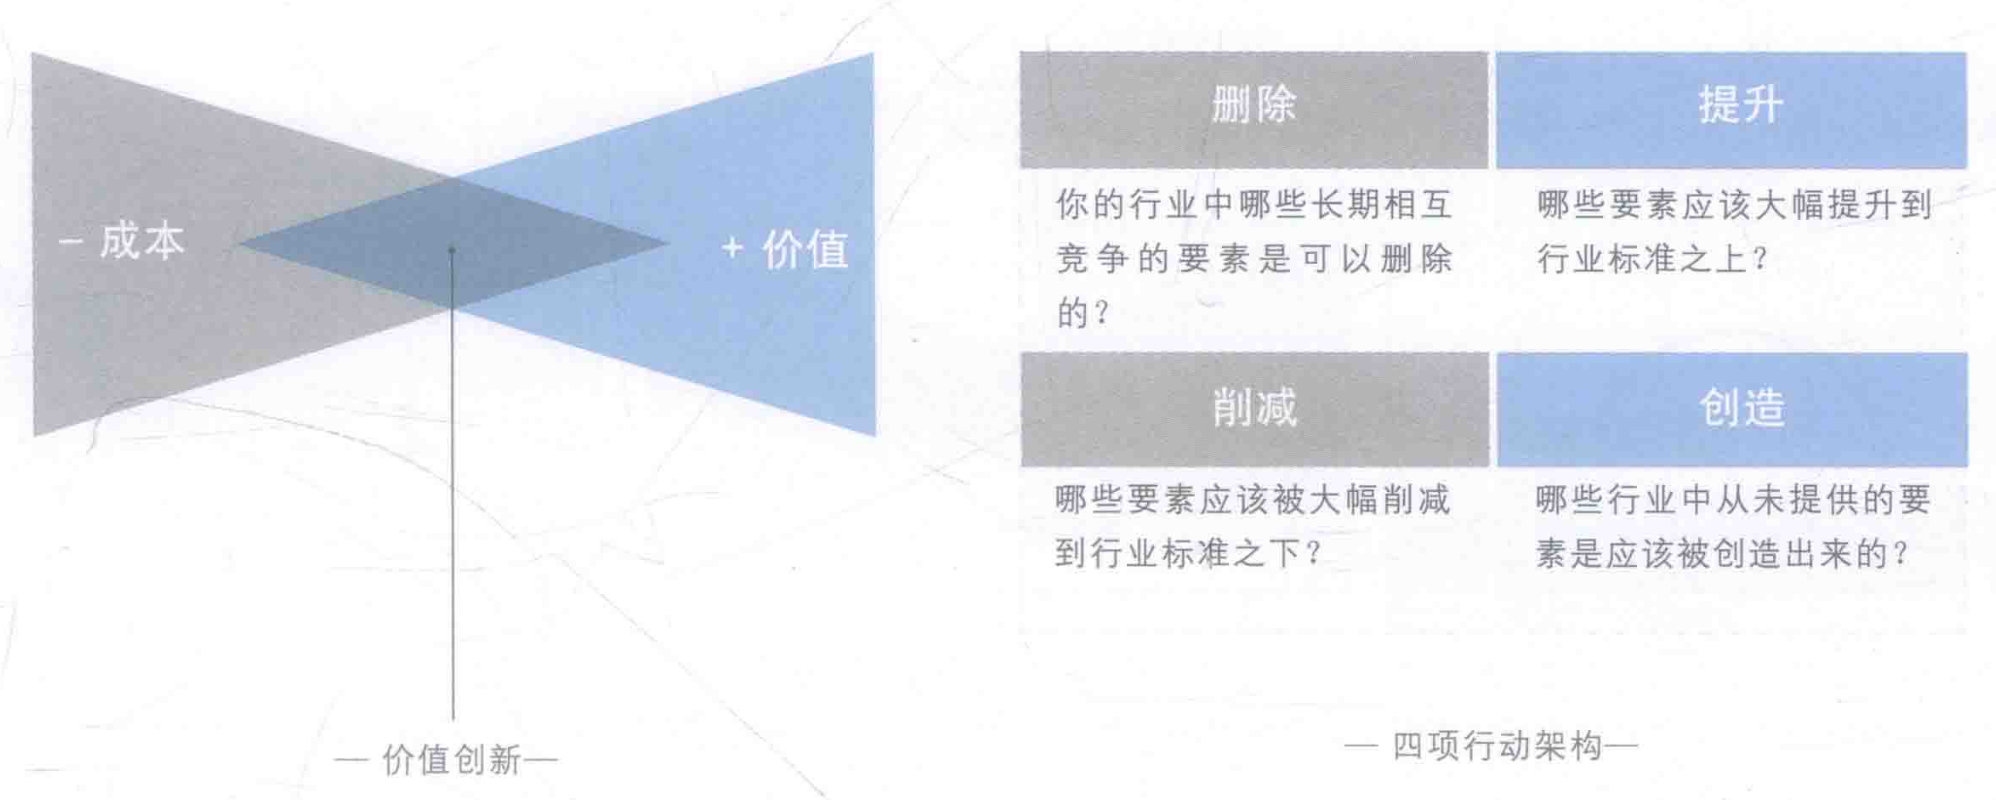
\includegraphics[width=0.6\textwidth]{img/蓝海战略.png}
    \vspace{-0.5em}
\end{figure}

整合蓝海战略框架和商业模式画布
\begin{itemize}
    \item 商业模式右半部关注价值、聚焦客户,左半部分关注成本和基础设施。右侧的改变回对左半部分产生影响
    \item 蓝海战略强调在增加价值的同时减少成本,通过删除和消减低价值产品或服务来降低成本,通过提升和创造对成本影响弱的高价值功能或服务来实现
    \item 二者的整合使得使用“四项行动架构”分析时能够更好地识别这些行动对商业模式其它模块的影响
\end{itemize}

\begin{figure}[H]
	\centering
	\vspace{-0.5em}
	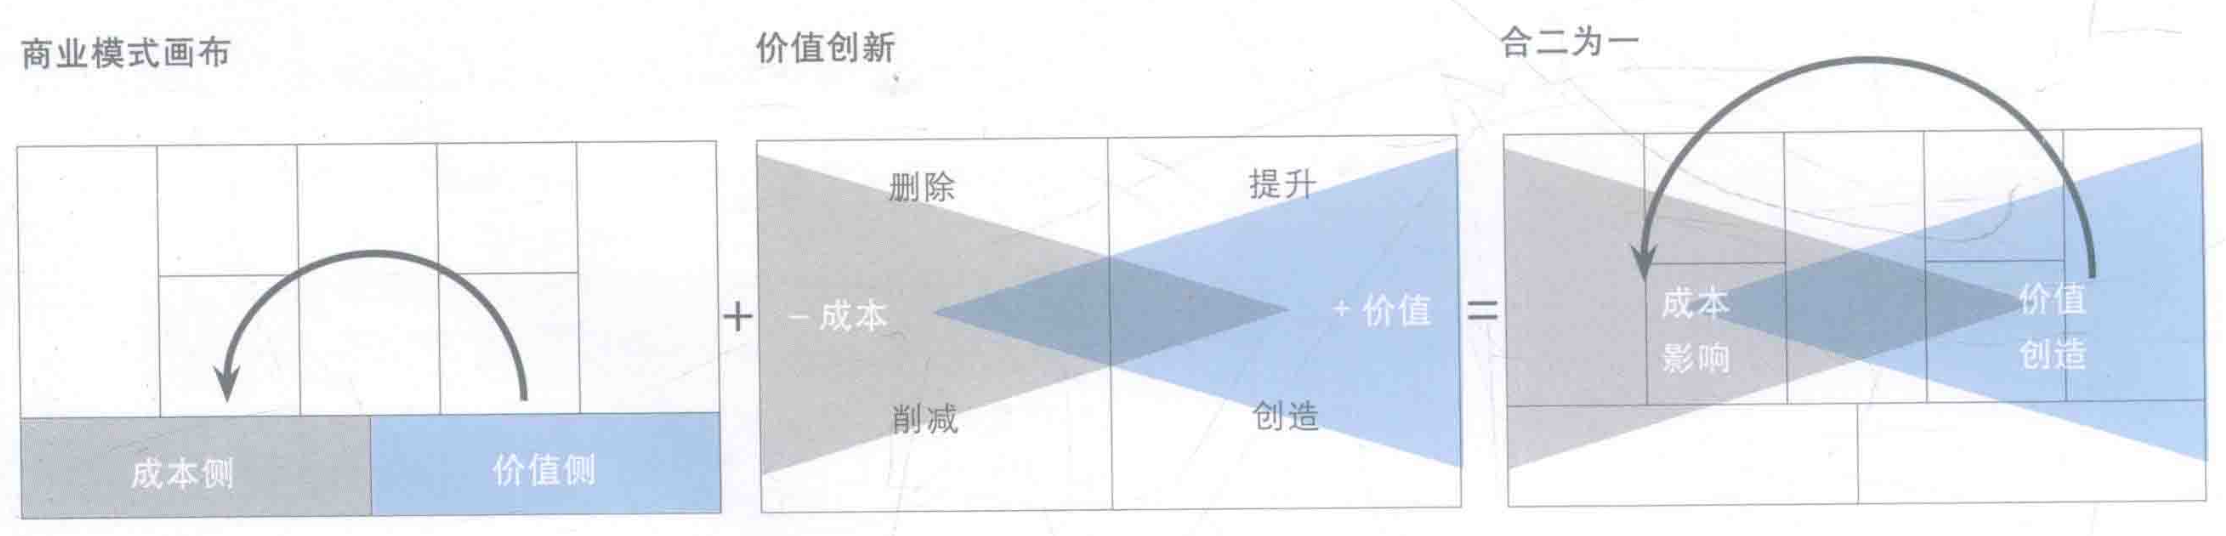
\includegraphics[width=0.9\textwidth]{img/整合蓝海战略框架和商业模式画布.png}
    \vspace{-0.5em}
\end{figure}

例:太阳马戏团
\begin{figure}[H]
	\centering
	\vspace{-0.5em}
	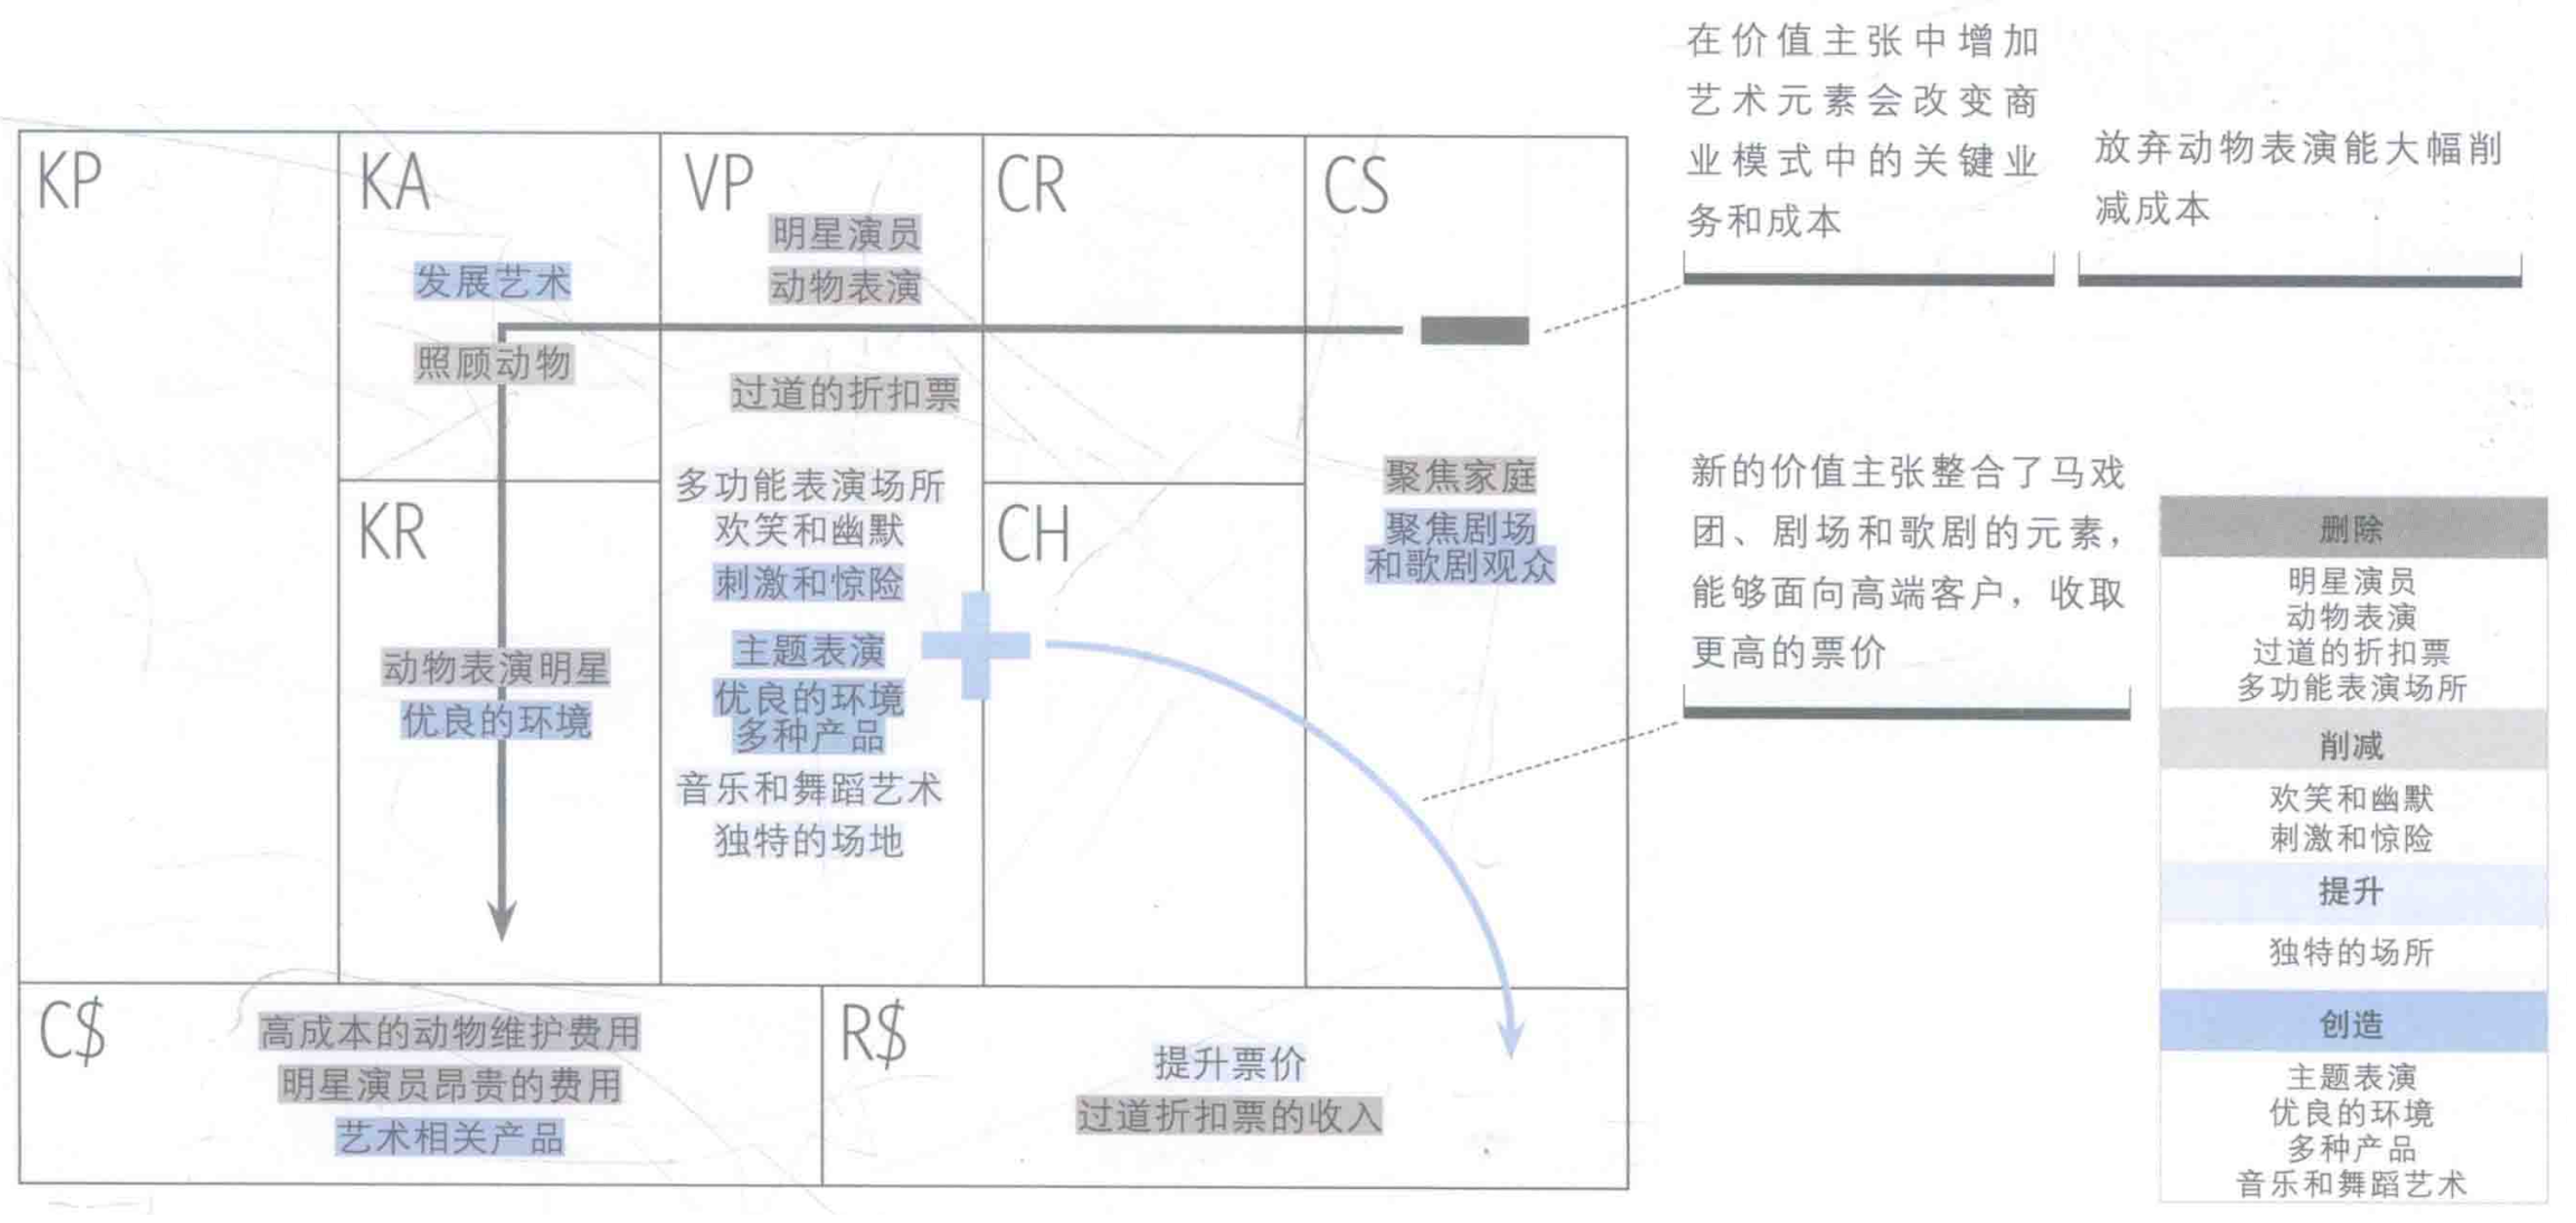
\includegraphics[width=0.85\textwidth]{img/太阳马戏团.png}
    \vspace{-0.5em}
\end{figure}

通过四项行动架构探究画布
\begin{figure}[H]
	\centering
	\vspace{-0.5em}
	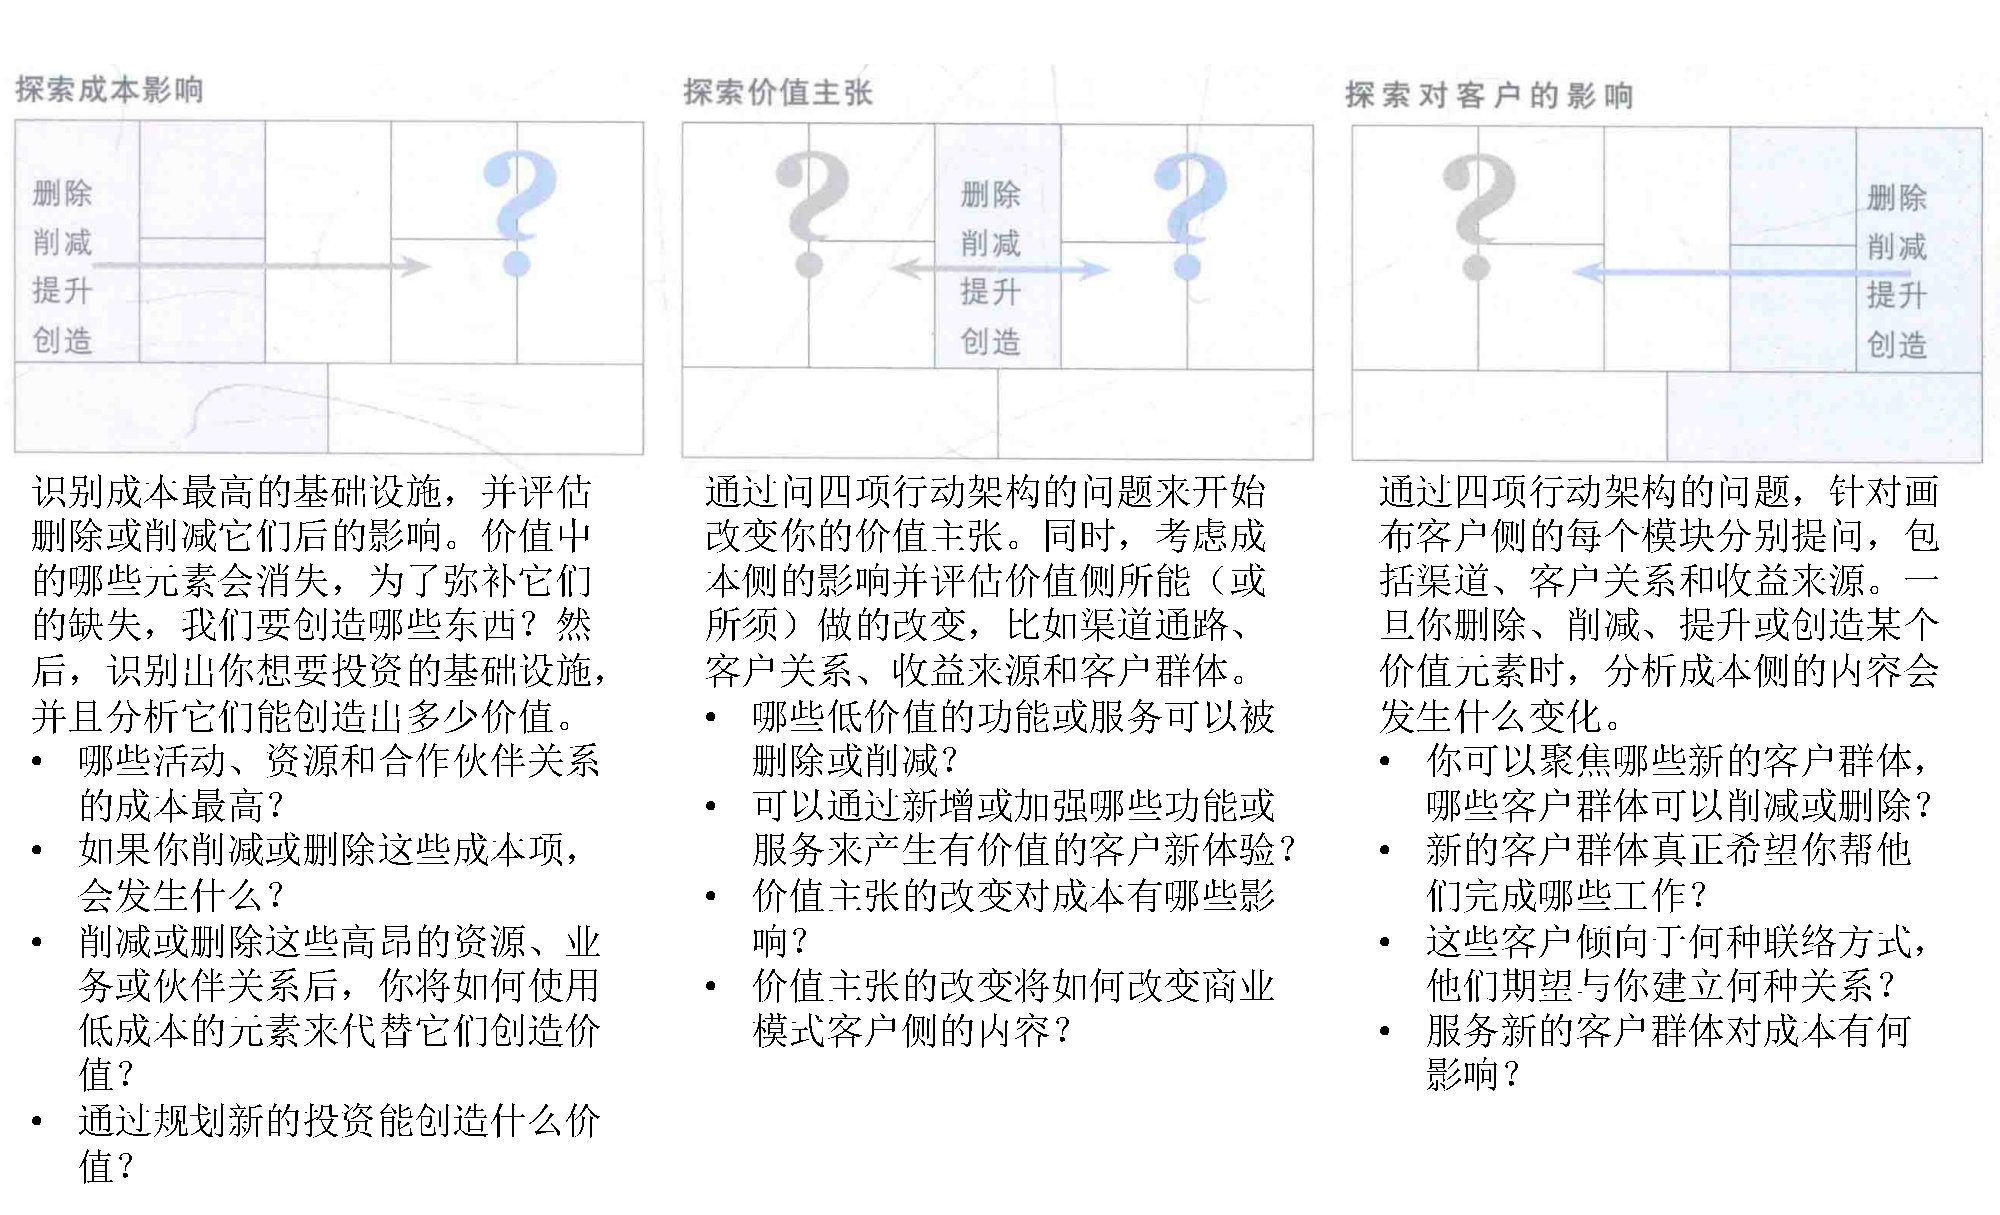
\includegraphics[width=\textwidth]{img/通过四项行动架构探究画布.pdf}
    \vspace{-0.5em}
\end{figure}


\subsection{管理多种商业模式}
成功应对如何在实施和管理新商业模式的同时维持现有的商业模式这个挑战的组织被称为:二元组织。

\begin{itemize}
    \item 组织的艰巨任务:如何在实施和管理新商业模式的同时维持现有的商业模式
    \begin{itemize}
        \item 将新商业模式剥离成一个独立的实体,或者成立独立的业务单元,或维持现状
        \item 拆分商业模式:基础服务、客户关系、新业务
    \end{itemize}
    \item 衡量是否拆分的双变量
    \begin{itemize}
        \item 两种模式冲突的严重程度
        \item 战略上的相似性
        \item 风险是值得我们考感的第三个变量。新的商业模式有多大风险会对现有的模式产生负面的影响,无论是品牌形象、收入、法律责任,还是其他方面
    \end{itemize}
\end{itemize}

\begin{figure}[H]
	\centering
	\vspace{-0.5em}
	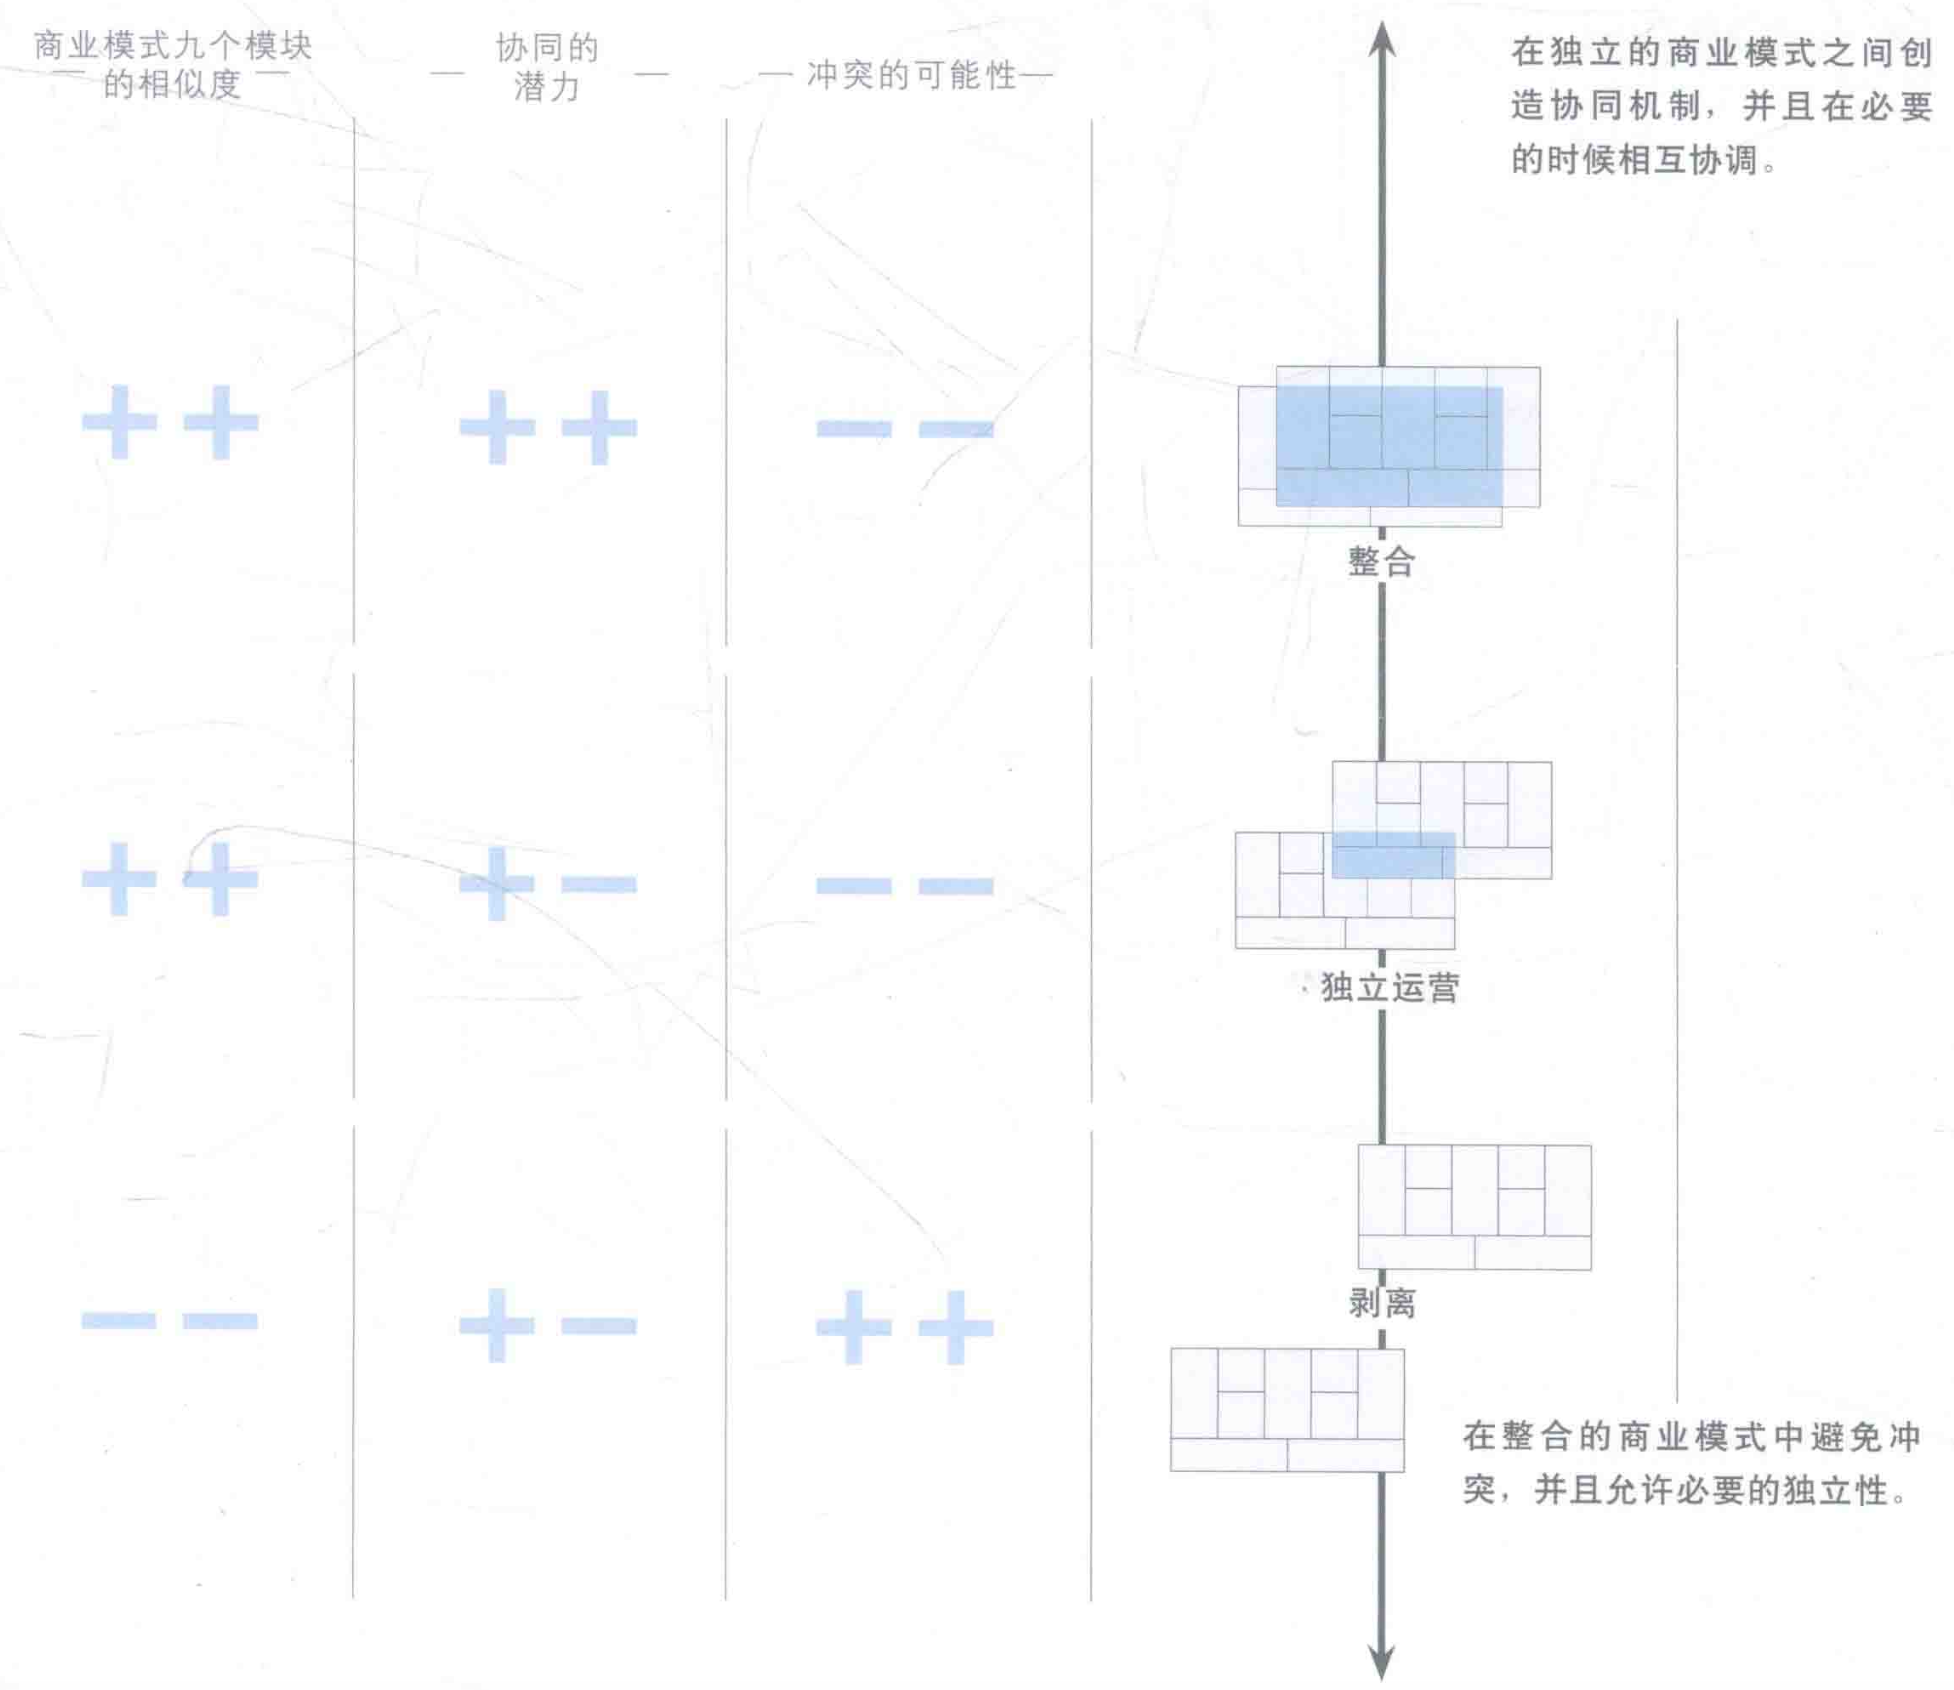
\includegraphics[width=0.6\textwidth]{img/管理多种商业模式.png}
    \vspace{-0.5em}
\end{figure}

例:SMH(后改名为SWATCH,斯沃琪)的SWATCH品牌的独立运营模式
\begin{figure}[H]
	\centering
	\vspace{-0.5em}
	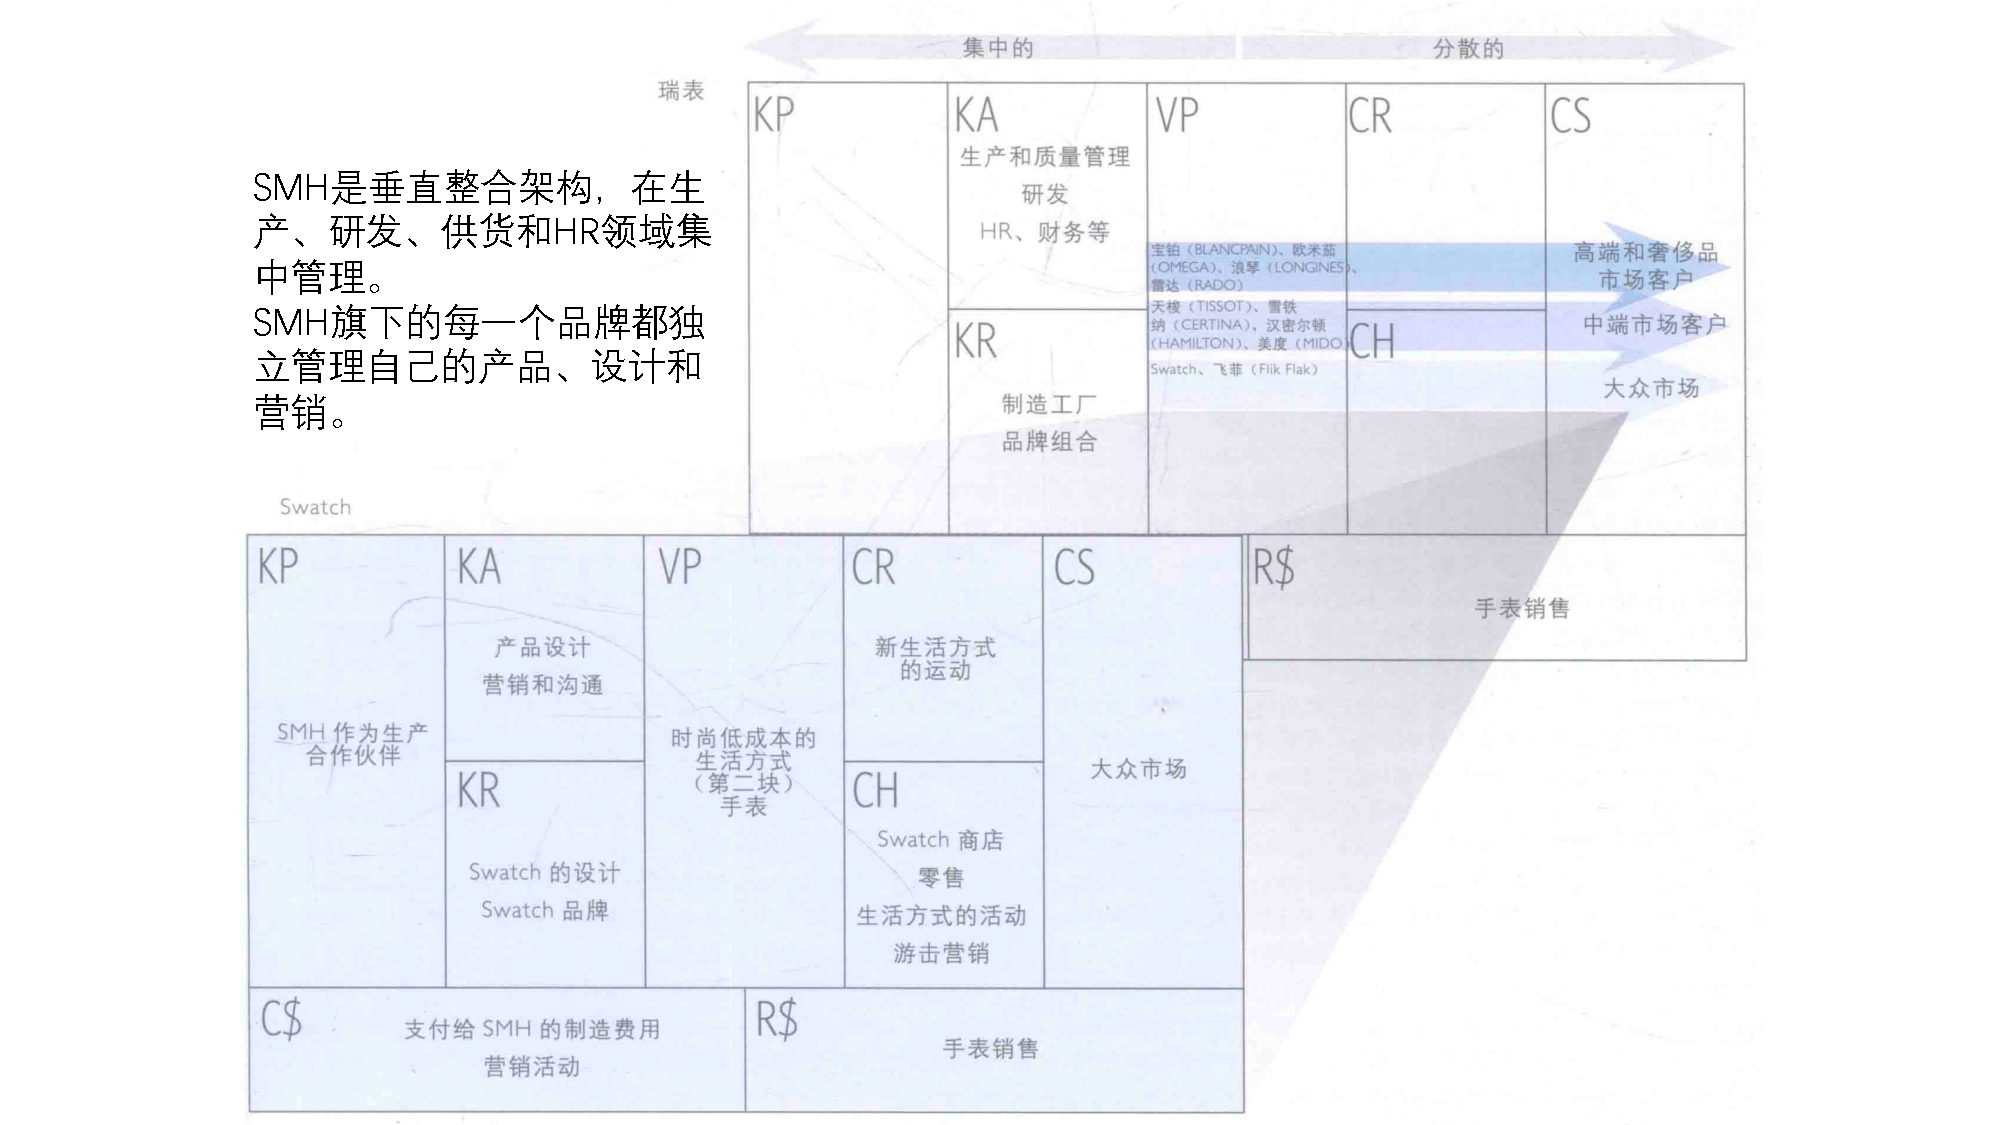
\includegraphics[width=0.7\textwidth]{img/SMH的SWATCH品牌的独立运营模式.pdf}
    \vspace{-0.5em}
\end{figure}

例:雀巢公司的咖啡商业模式组合
\begin{figure}[H]
	\centering
	\vspace{-0.5em}
	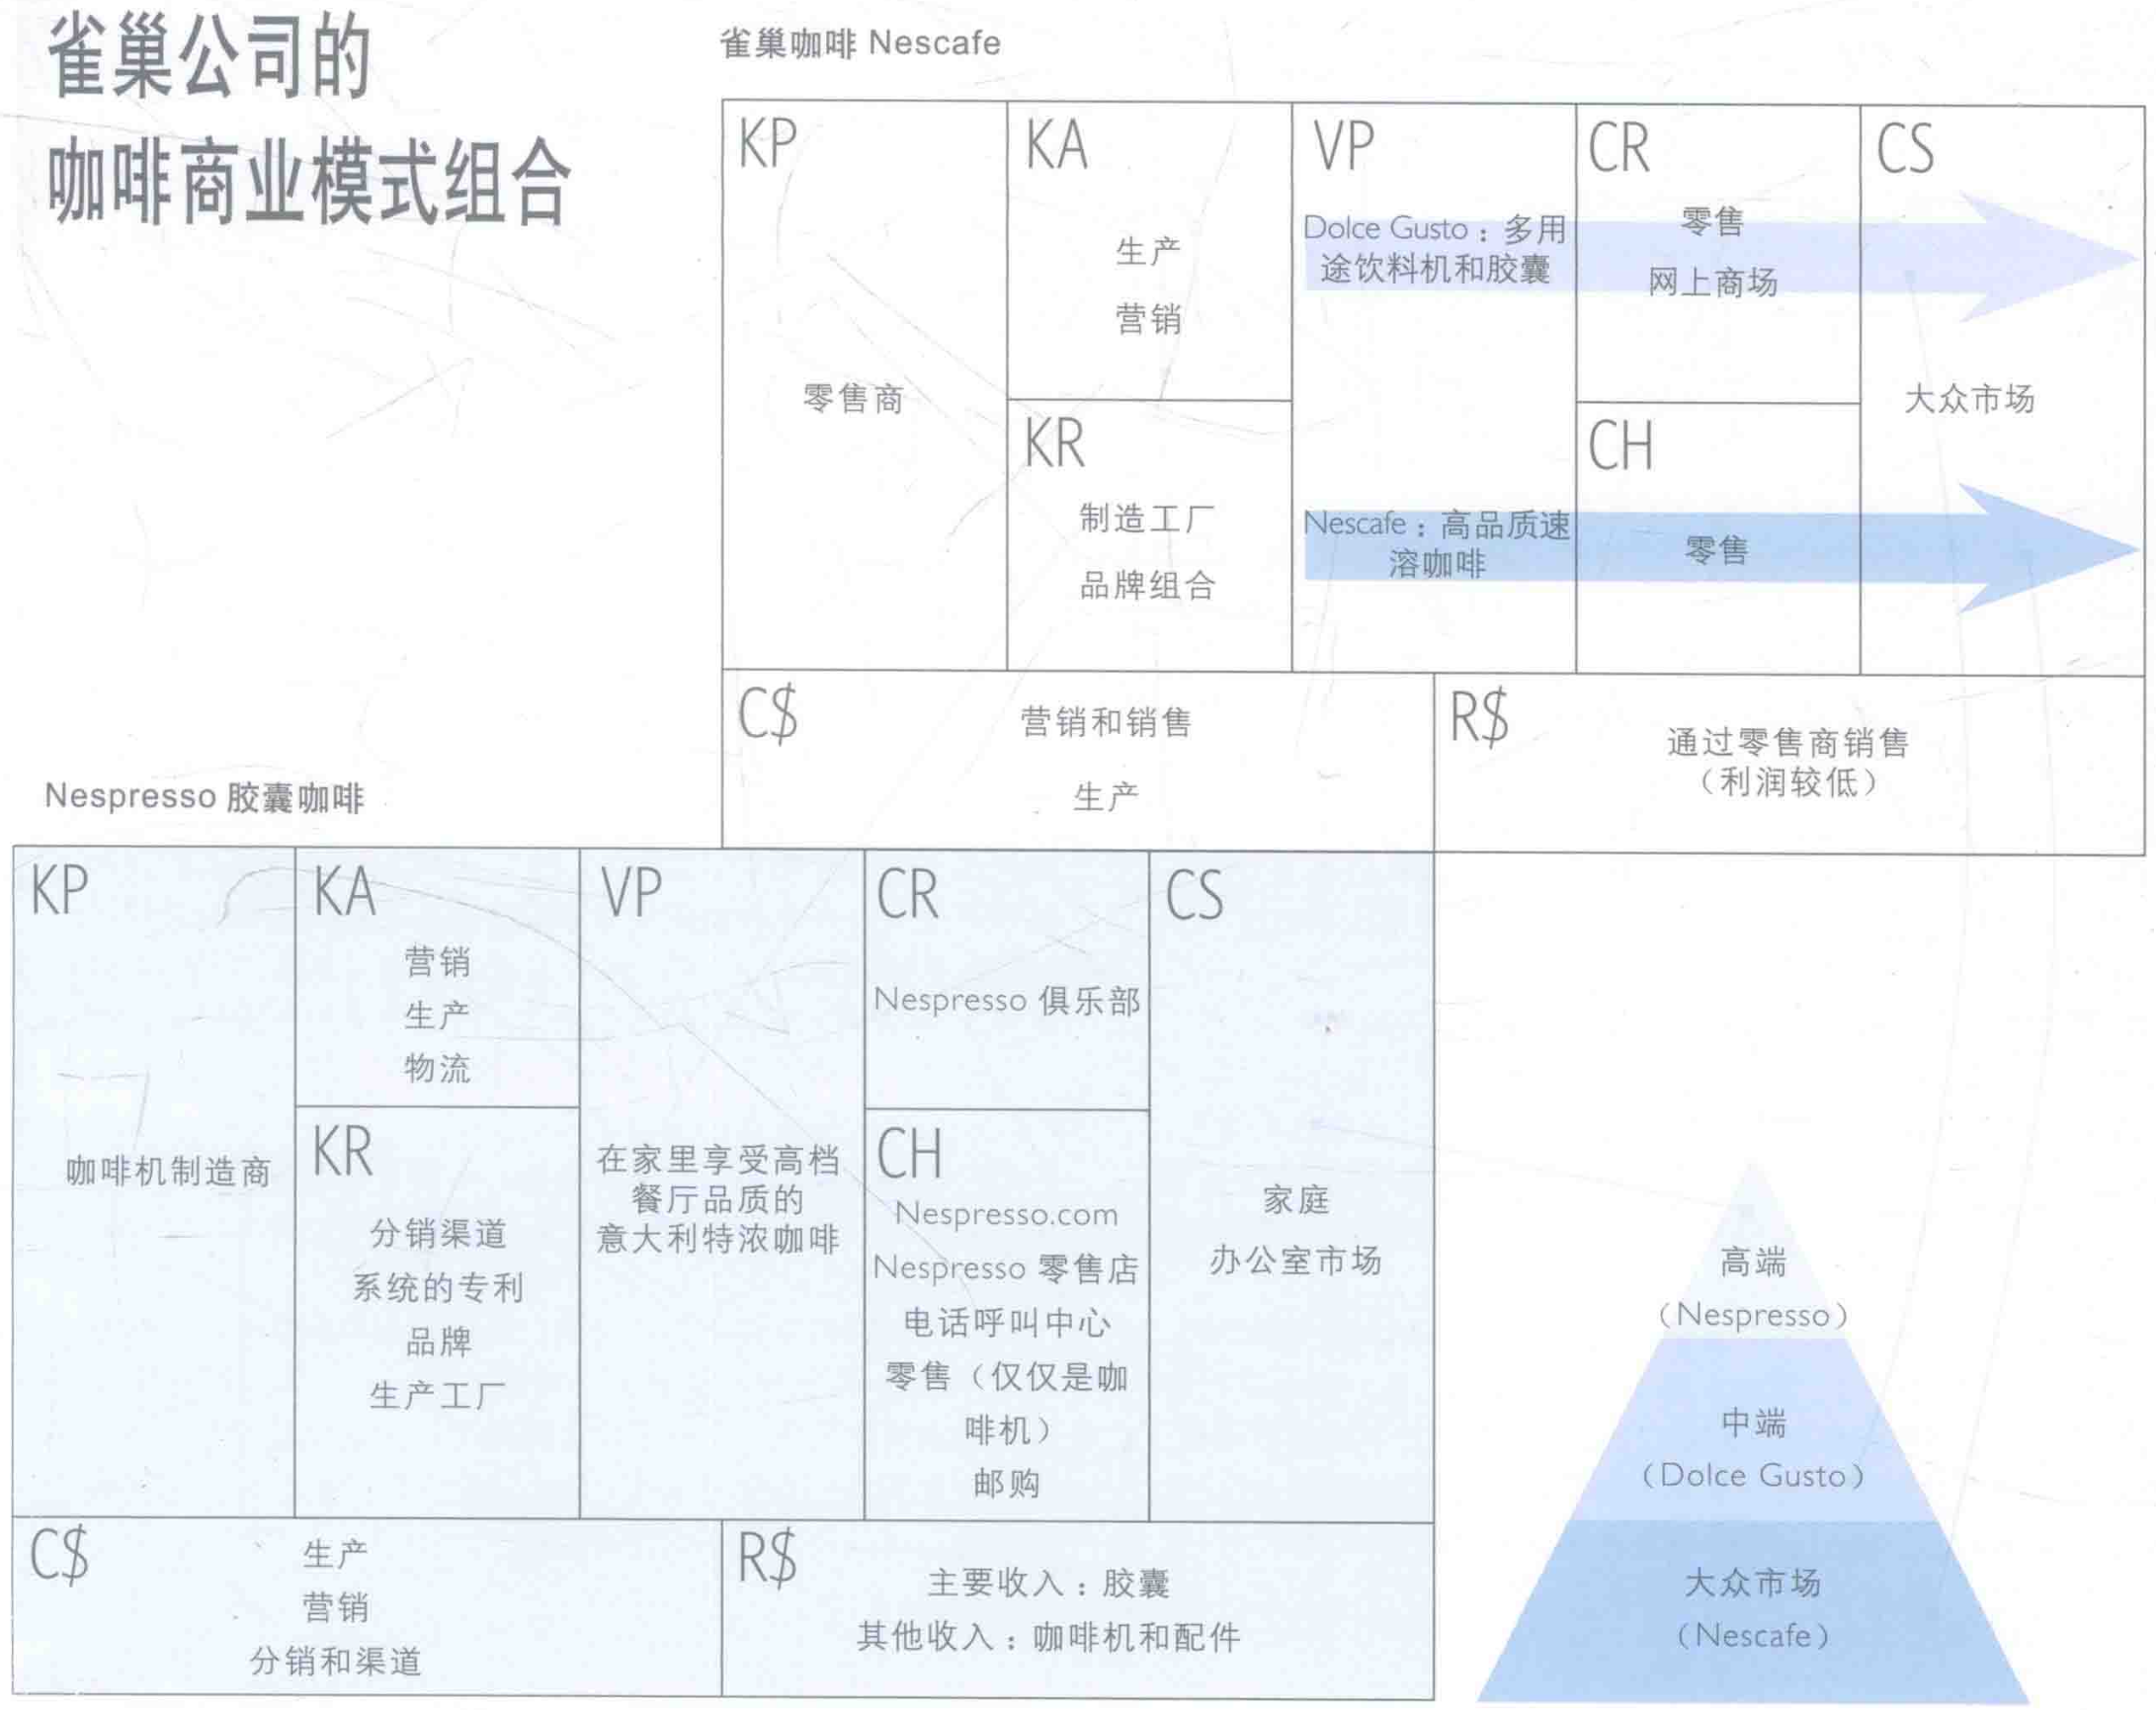
\includegraphics[width=0.7\textwidth]{img/雀巢公司的咖啡商业模式组合.png}
    \vspace{-0.5em}
\end{figure}

例:戴姆勒公司Car2go的商业模式
\begin{figure}[H]
	\centering
	\vspace{-0.5em}
	\includegraphics[width=0.7\textwidth]{img/戴姆勒公司Car2go的商业模式.png}
    \vspace{-0.5em}
\end{figure}
	\section{商业模式设计流程}

商业模式设计流程有五个阶段:\textbf{动员}、\textbf{理解}、\textbf{设计}、\textbf{实施}和\textbf{管理}。

\subsection{商业模式创新的基本出发点}

商业模式创新的目的无非以下四种:
\begin{itemize}
    \item 满足市场:满足未被响应的市场需求。比如印度塔塔汽车、私人飞机租赁商奈特捷、孟加拉乡村银行、鲁鲁自助出版社(lulu.com)。
    \item 投放市场:将新技术、产品或服务推向市场,或者开发现有的知识资产。比如施乐914型 复印机、Swatch手表、Nespresso胶囊咖啡、红帽子开源软件公司。
    \item 改进市场:改进或者颠覆当前的市场。比如戴尔电脑公司、瑞士盈丰私人银行、任天堂Wii、宜家、印度巴蒂电信、Skype、瑞安航空、亚马逊零售业务、从事电动汽车电池服务的乐土公司。
    \item 创造市场:创造一种全新的业务。比如大来卡就餐信用卡、谷歌。
\end{itemize}

上述过程所面对的挑战有:
\begin{itemize}
    \item 找到正确的模式
    \item 在全面启动前验证该模式
    \item 诱导市场接受新的模式
    \item 根据市场的反馈不断调整该模式
    \item 管理不确定因素
\end{itemize}

对于成熟企业来说,商业模式创新活动通常反映了它当前的商业模式和组织结构。它们的创新通常会缘 于以下四种动机之一:
\begin{itemize}
    \item 被动反应:由当前商业模式的危机而引发。比如20世纪90年代的IBM、任天堂的Wii、劳斯莱斯喷气引擎。
    \item 调整适应:调整、改进或者捍卫现有的商业模式。比如诺基亚的“与音乐同行Comeswithmusic”项目、宝洁公司的开放创新计划、建筑行业产品制造商喜利得公司。
    \item 扩张:发布一项新技术、产品或者服务。比如Nespresso胶囊咖啡、20世纪60年代的施乐914复印机 、iPod/iTunes
    \item 主动开拓:为未来做准备。比如戴姆勒的Car2go、亚马逊云计算服务AmazonWebService。
\end{itemize}


上述过程所面对的挑战有:
\begin{itemize}
    \item 对新的模式产生欲望
    \item 新老模式之间的拉通
    \item 管理既得利益
    \item 聚焦长远利益
\end{itemize}

\subsection{设计态度}
\begin{itemize}
    \item 创新的参与者必须愿意投入大量的时间和经历去探索很多的可能,而不是过早地采用某一种解决方案,时间的投入会得到回报的,会因此获得更强大的新商业模式,确保未来的增长。
    \item 寻找真正出色的方案,而不是修饰一个很快得到的方案。
\end{itemize}

\begin{figure}[H]
	\centering
	\vspace{-0.5em}
	\includegraphics[width=0.7\textwidth]{img/设计曲线.png}
    \vspace{-0.5em}
\end{figure}

\subsection{商业设计流程的五个阶段}

\begin{figure}[H]
	\centering
	\vspace{-0.5em}
	\includegraphics[width=\textwidth]{img/商业模式设计流程.pdf}
    \vspace{-0.5em}
\end{figure}


	\section{商业模式展望}

下面将简要地讨论五个课题:
\begin{itemize}
    \item 第一个课题考察超越经济利益的商业模式:商业模式画布如何在公共服务和非营利组织中推动商业模式创新。
    \item 第二个课题探讨计算机辅助的商业模式设计相对于笔头设计的优势,允许我们更复杂地操纵商业模式元素。
    \item 第三个课题讨论商业模式和商业计划之间的关系。
    \item 第四个课题则指出在初创组织或者成熟组织中执行商业模式的时候会出现的问题。
    \item 第五个课题考察如何更好地协同商业模式和IT。
\end{itemize}

\subsection{超越经济利益的商业模式}
\begin{itemize}
    \item 每一个组织都有一个商业模式,即便它并没有“商业”属性
    \item 为非盈利组织、慈善机构、公共服务实体和以盈利为目的的社会投资机构服务
    \item 主要讨论的是非盈利组织的的商业模式,这种我们更倾向于叫做“企业模式”
    \begin{itemize}
        \item 第三方资助的企业模式(比如公益组织、慈善组织、政府组织)
        \item 有强烈的环境和社会使命的“三重损益商业模式:“三重损益”指的是计算环境、社会和财务成本
    \end{itemize}
\end{itemize}


\subsection{计算机辅助的商业模式设计}
\begin{figure}[H]
	\centering
	\vspace{-0.5em}
	\includegraphics[width=0.65\textwidth]{img/计算机辅助的商业模式设计.pdf}
	\vspace{-0.5em}
\end{figure}

\subsection{商业模式和商业计划}
\begin{figure}[H]
	\centering
	\vspace{-0.5em}
	\includegraphics[width=\textwidth]{img/商业模式和商业计划.pdf}
	\vspace{-0.5em}
\end{figure}

\subsection{在组织中执行商业模式}
组织中必须相互协同的五个领域:战略、架构、流程、激励和人员。我们将商业模式放在这个星型的中央,好像一个“引力中心”牢牢抓住这五个领域。
\begin{figure}[H]
	\centering
	\vspace{-0.5em}
	\includegraphics[width=0.6\textwidth]{img/在组织中执行商业模式.png}
	\vspace{-0.5em}
\end{figure}


\subsection{IT与业务的协同}
\begin{figure}[H]
	\centering
	\vspace{-0.5em}
	\includegraphics[width=0.85\textwidth]{img/IT与业务的协同.pdf}
	\vspace{-0.5em}
\end{figure}
	
\end{document}


